%!TEX TS-program = xelatex
%!TEX encoding = UTF-8 Unicode

\documentclass{harvard-thesis}
\let\oldcentering\centering

\usepackage{breqn}
\usepackage{hyperref}
\usepackage{amsmath}
\usepackage{nicematrix}
\usepackage{array,multirow}
\usepackage{bm}
\usepackage{url}
\usepackage{longtable}
\usepackage{caption}
\usepackage{alphabeta}
\usepackage{lipsum}  
\usepackage{tabularx}
\usepackage{pdfpages}
\usepackage{pdflscape}
\usepackage{epigraph}
\usepackage{graphicx}
\usepackage[bb=boondox]{mathalfa}
\usepackage[symbols,automake=true,nogroupskip]{glossaries-extra} 
% AAD ALL THIS THE LAST TIME WE RAN IT ,section=chapter*
%,numberedsection=false,nonumberlist,,toc=false
\usepackage{fontspec}
\usepackage{comment}
%\usepackage[section]{placeins}

\newcommand\invisiblesection[1]{%
  \refstepcounter{section}%
  \addcontentsline{toc}{section}{\protect\numberline{\thesection}#1}%
  \sectionmark{#1}}
% headers

\usepackage[doi=false,hyperref,backend=biber,backref,backrefstyle=none,isbn=false,eprint=false,maxnames=9,style=nature,url=false]{biblatex}
\usepackage{scrhack}
\newbibmacro{string+doi+url+isbn}[1]{%
  \iffieldundef{doi}{%
    \iffieldundef{url}{%
      \iffieldundef{isbn}{%
        \iffieldundef{issn}{%
          #1%
        }{%
          \href{http://books.google.com/books?vid=ISSN\thefield{issn}}{#1}%
        }%
      }{%
        \href{http://books.google.com/books?vid=ISBN\thefield{isbn}}{#1}%
      }%
    }{%
      \href{\thefield{url}}{#1}%
    }%
  }{%
    \href{http://dx.doi.org/\thefield{doi}}{#1}%
  }%
} % Adds hyperrex to title. https://tex.stackexchange.com/questions/48400/biblatex-make-title-hyperlink-to-dois-url-or-isbn

\newbibmacro{string+doi}[1]{%
  \iffieldundef{doi}{\iffieldundef{url}{#1}{\href{\thefield{url}}{#1}}}{\href{http://dx.doi.org/\thefield{doi}}{#1}}}	
\DeclareFieldFormat[article]{title}{\usebibmacro{string+doi}{#1}}    
    
\AtEveryBibitem{%
  \clearfield{issn} % Remove issn
  \clearfield{doi} % Remove doi
  %\clearfield{pages} % Remove pages
  \clearfield{month}
  \clearfield{abstract}
}
\addbibresource{references.bib}


\DeclareCaptionJustification{justified}{\justifying}
\captionsetup{justification=justified}
\makeglossaries
\loadglsentries{Glossary}

\geometry{
    paper=b5paper,
    inner=20mm,         % Inner margin
    outer=30mm,         % Outer margin
    bindingoffset=10mm, % Binding offset
    top=25mm,           % Top margin
    bottom=28mm,        % Bottom margin
    %showframe,         % show how the type block is set on the page
}


\newcommand{\mean}[1]{\left\langle #1\right\rangle}
\newcommand*{\img}[1]{%
    \raisebox{-.3\baselineskip}{%
        \includegraphics[
        height=\baselineskip,
        width=\baselineskip,
        keepaspectratio,
        ]{#1}%
    }%
}
\renewcommand{\arraystretch}{1.2} %<- modify value to suit your needs
\begin{document}

%---------------------------------------------------------------------------
%	FRONT MATTER
%--------------------------------------------------------------------------

\includepdf[pages =-,offset=0 0]{frontmatter/official_cover.pdf}
\pagenumbering{roman}
\abstractpage
\acknowledgments
%\printglossary[type=symbols,style=long,title={List of Symbols and Abreviations}]
\publicationspage
\dedicationpage

%---------------------------------------------------------------------------
%	TABLE OF CONTENTS AND LISTS
%---------------------------------------------------------------------------
\tableofcontents
\setcounter{tocdepth}{2}
\setcounter{secnumdepth}{2}
\newpage
\thispagestyle{empty} % first page of TOC without numbering
%\addtocontents{toc}{\protect\thispagestyle{empty}} % second page of TOC without numbering
    \newpage 
    \ % The empty page
    \newpage
    
%%%%%%%%%% lists
\addcontentsline{toc}{section}{List of Tables}
\listoftables
\cleardoublepage
\addcontentsline{toc}{section}{\listfigurename}

\listoffigures
\newpage
\thispagestyle{empty}
    \newpage 
    \ % The empty page
    \newpage
\pagenumbering{arabic}

%---------------------------------------------------------------------------
%	CONTENT CHAPTERS
%---------------------------------------------------------------------------
%\setcounter{page}{1}
\chapter{Introduction}\label{chp:intro}

Imagine you are given a mechanical duck. It quacks and moves awkwardly. At a certain point, you take it apart and study all the gears and pulleys that make it up, enabling you to understand how it works. By getting more ducks, you realize that all gathered together simply quack and walk like the first one. Nothing more. However, if you get your hands on a real bird, e.g.a starling, it is a completely different story. Instead of taking it apart (please do not), you observe it and eventually learn something about it, such as its diet and sleep patterns. But when you encounter a flock of starlings, you realize that studying a single bird does not prepare you for the emergent behavior of the group. The flock can create intricate patterns in flight, something that you would not have imagined from observing a single starling (Figure~\ref{fig:intro:duck}). \\

\begin{figure}[h]
    \centering
    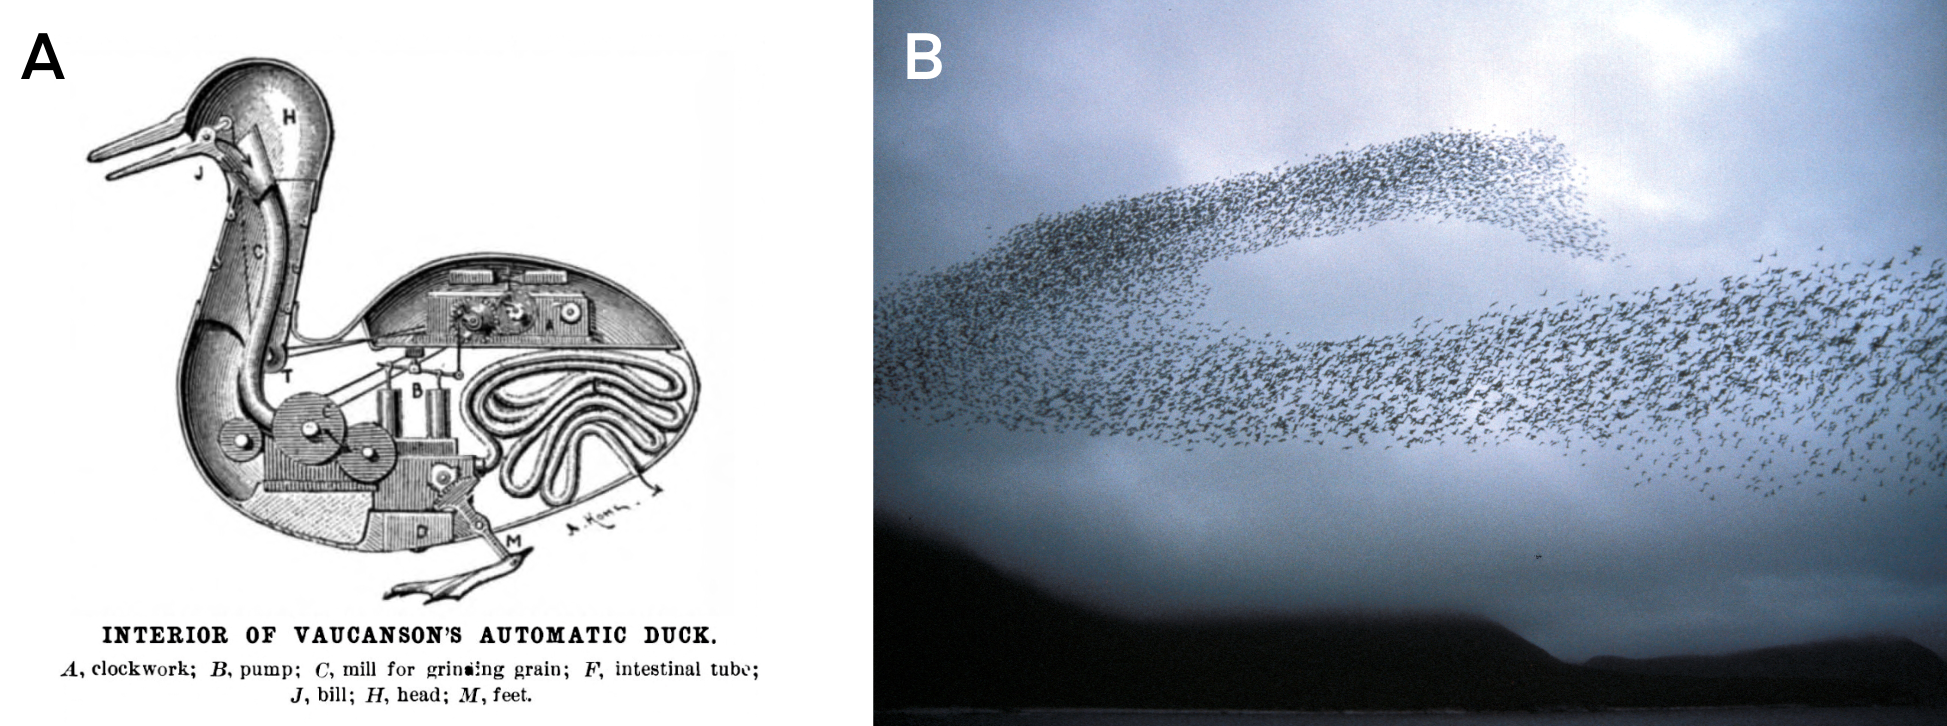
\includegraphics[width=\textwidth]{figures/intro/duck_flocking.png}
    \caption[Reductionism and emergence]{The digestive duck (Panel A) has become a symbol of reductionism, which states that the behavior of every system could be described as the sum of its individual components' contributions. A flock of birds, on the other hand, illustrates the concept of collective animal behavior (Panel B). It is considered an emergent behavior that arises from individuals following simple rules without any central coordinator. Images from Wikimedia Commons under public domain.}
    \label{fig:intro:duck}
\end{figure}

The philosophical attitude underneath the approach taken with the mechanical duck is called reductionism. It claims that systems can be explained by reducing them to their fundamental components. Reductionism has been highly successful in some scientific fields, especially in physics. However, this approach fails to explain all the rich behavior of some physical systems, such as the spontaneous symmetry breaking observed in many-body physics \cite{anderson1972more}. These systems exhibit irreducible properties at all scales that cannot be explained by studying their individual components alone, like the swarm behavior of a flock of starlings. Emergent phenomena are present also in other fields such as ecology and biology. For example, we find the formation of ant colonies (a population of ants capable of coordinating social and complex tasks without a central controller), the creation and maintenance of ecosystems (which are composed of a multitude of different interacting species), or the synchronization of fireflies. There are examples from a social standpoint too. The richness of human interactions is evidenced by viral information spreading, economic growth, or the evolution of language. \\

The ubiquity of emergent properties makes it apparent that many systems are more than the sum of their parts, and a classic approach does not work with them. As P. W. Anderson stated in this seminal 1972 paper \cite{anderson1972more}, ``the ability to reduce everything to simple fundamental laws does not imply the ability to start from those laws and reconstruct the universe''. It is at this point where complex systems science comes into play. Adopting an interdisciplinary approach, complexity science investigates how emergent properties arise and how they affect the behavior of the system as a whole. Drawing on concepts and tools from physics, mathematics, biology, and computer science, to name but a few, it aims to better understand the complexity of the world around us. However, despite the large number of systems we can claim to be complex, an operative definition of complex systems has been elusive. \\

The term's ambiguity should not cause concern \cite{horgan1995complexity}, since other crucial concepts still generate significant debate regarding their formal scientific definition. These concepts include consciousness, sustainability, and life. As with the elusive concept of life \cite{schrodinger1992life}, instead of attempting to provide a scientific definition of complexity, we will outline the essential characteristics of typical complex systems \cite{de2019complexity}. This will enable us to identify and differentiate them from systems that we might classify as very complicated, but not necessarily complex, such as the mechanical duck. As mentioned earlier, typical  complex systems exhibit emergence and self-organization, which happens when interactions between their (usually) many components produce a global pattern of behavior. These interactions are highly heterogeneous and may generate new information, making it challenging to study isolated components or accurately predict future outcomes. The unpredictable long-term behavior that complex systems display is often driven by their non-linear dynamics and the presence of phase transitions. Complex systems may adapt their interactions to changing environmental conditions, as opposed to merely approaching a steady state. Given the emphasis on interactions, it is not surprising that the main challenge of complexity science is to understand how the structure of these interactions gives rise to the system's behavior as a whole.\\

%Here, paragraph of why ecology and social science can be seen as complex systems:
Certainly, the characteristics of complexity discussed in the previous paragraph can be observed in a wide variety of situations, including natural and social systems. Natural ecosystems are considered paradigmatic examples of complex systems due to their adaptative power, presence of patterns, and their diversity of species and interactions. Precisely this remarkable biodiversity and heterogeneity make them a paradigmatic illustration of complexity. \cite{levin1998ecosystems}.  It is not surprising then that, in the young field of ecology \cite{ghazoul2020ecology}, complex systems' approaches have been taken to understand the functioning of species-rich communities. To gain these insights, ecosystems are often described as complex networks, rather than just individual pairwise interactions, to examine their structure and how it affects their dynamics. Depending on the research question, this network description can be done at several levels of organization: individual-based networks, followed by species-based, and finally, clade-based networks \cite{guimaraes2020structure}. Studying complex systems at different scales is important because it provides us with different perspectives on the system's behavior. Moreover, recent approaches at a macroscopic level have highlighted the presence of statistical patterns in community structure, which indicate the presence of fundamental principles or laws of nature \cite{brown1995macroecology,brown2004toward}. These patterns manifest as scaling relationships and recurrent distributions with similar parameters across different communities \cite{west1997general}. Exploring ecosystems as complex adaptive systems allows us to address some central questions, especially regarding the relationships between structure and functioning, the existence of universal biodiversity patterns, and the mechanisms that determine them \cite{levin1998ecosystems}.\\

% ECO   in coexistence: statisctical physics, random matrix theory and nonlinear dynamics . No decir todo el rato coexistence, tambien persistence
% social systems e interdiscipliplinariedad, paper Computational Social Science ≠ Computer Science + Social Data 

% SOCIAL: transportation airports... 
Complexity is pervasive in social phenomena as well.  A typical social system is composed of agents whose collective behavior is not usually manifested in the properties of the single constituents. For example, it would be inadequate to use the trajectory of one individual as the only reference to study mobility in a city, and as a case in point, a city itself is much more than the aggregation of its buildings and people. There are plenty of cases in which the lens of complex systems has deepened our understanding of human activity. In this context, the spreading of diseases has been a problem extensively addressed within the complex systems community, developing more and more complete models that integrate simultaneous processes \cite{soriano2018spreading}, and anticipate the advance of outbreaks \cite{mazzoli2023spatial}. Moreover, power grid fluctuations \cite{martinez2023dynamical}, pedestrian dynamics \cite{zuriguel2020contact} and the impact of road disruptions have been modeled to improve overall system performance \cite{bassolas2020scaling}. Lastly, in the context of social relationships,  large advances have been made towards explaining the arise of cooperation \cite{axelrod1981evolution}, which has been a major challenge in human behavior and other disciplines \cite{Nowak2006EvolutionaryDynamics}.\\

Ecological and social systems are just two examples among all the contexts that can be regarded as complex. Indeed, they appear in many scientific domains, and hence the traditional methodology of each domain is not enough to fully explore complex systems in a unified way. Instead, computational modeling and mathematical tools are required and developed to explore the structure and evolution of complex systems. Among these methods, two frameworks have proven extremely useful, which we will adopt in this thesis. One is that of complex networks, which connect the interactions’ architecture with the collective dynamics. For example, by describing the relationship between pollinators and plants as networks, it has been found that their nested structure increases species persistence and resilience \cite{cota2019echo}.  From a social perspective, the emergence of cooperation also depends on the connectivity of the network of connections \cite{raducha2022coordination}. Political polarization and the spread of diseases have also found a network description very profiting. Complex systems may have processes working at different spatial and temporal scales. Thus, the other perspective is that of looking at the systems from different scales to gain a complete understanding of the interplay of different processes. Ultimately, a macroscopic description of the systems can characterize and explain statistical patterns that span different orders of magnitude. In linguistics, for example, it is well-known Zipf’s law, which describes the word frequency distribution in the vast majority of linguistic corpora  \cite{zipf1999psycho}. Analogously, the metabolic rate of organisms varies as a power law with temperature and body size \cite{brown2004toward}, and, within social phenomena, the production of goods or consumption of energy scale nonlinearly as a function of city size \cite{west2017scale}. \\

Furthermore, studying complex systems at different scales allows us to understand the contribution of each level of description to the overall dynamics. Therefore, we will address our following challenges from different scales of description. By taking a more holistic approach to complex systems modeling, we can gain a better understanding of how various interactions influence one another and how emergent properties arise. This, in turn, can inform our understanding of real-world systems and help us to develop more accurate predictive models. \\

\section{Our contributions}
Despite significant advances in complex systems modeling, there is still much to explore. This thesis focuses on the challenges related to ecological interactions. Since there is a current trend to develop ecological models that capture the heterogeneity of these interactions, a complex systems approach is suitable for studying them. Then, the first goal of this thesis is to investigate how emergent properties, particularly the coexistence of multiple agents, are affected by the inclusion of space, several interactions simultaneously, and different interaction topologies. \\

%most of these models fail to capture all the heterogeneity of their interactions. Typically, these models consider only one type of interaction at a time, ignoring potential interdependencies between different types and the effects of time and space on them. In thesis, we aim to address these limitations by exploring how emergent properties, in particular the coexistence of many different agents, are affected by these considerations. \\

\subsection{Bridging ecological and social systems}\label{chp:intro:bridge}
 The versatility of the complexity paradigm allows it to address a wide range of problems across different contexts with a common language, borrowing concepts and models from different types of complex systems. We can adopt established solutions from other systems to tackle problems in our own settings. Specifically,  one can examine the similarities between ecological systems and human interactions in the context of online social networks (OSNs). They have revolutionized how we communicate and process information, but also have brought to light the cognitive limitations of our brains. We have gone from a situation where we only received information from a few broadcast sources to being inundated with millions of messages demanding our attention. As a result, there has been an acceleration of social dynamics \cite{lorenz2019accelerating}, and the concept of ``competition for attention'' has become commonplace. Furthermore, OSNs are designed to capture and retain our attention by providing instant gratification \cite{fareri2014social,malik2016gratification} and reinforcing feedback \cite{sherman2018brain}. These limitations, combined with the vast amount of information produced every second, have resulted in competition between ideas/memes for visibility, leading users to adopt various strategies to increase the likelihood that their messages will be read. \\

The strong emphasis on how competition shapes information communications and on how users respond to it has inspired researchers to draw an analogy between natural and social systems \cite{borge2017emergence,lorenz2019accelerating,palazzi2021ecological,plata2021neutral,calleja2021quantifying,tovo2021upscaling}. Actors (like users and memes) of OSNs are seen as species of ecological communities that aim to maximize their abundance --visibility for users, popularity for memes--, and that are competing for a limited resource: the individuals' attention. Furthermore, the communication strategies adopted by the users can be interpreted in ecological terms too: posting specific hashtags to provide context to users' messages can be represented as mutualism, as it favors both visibility of users and the growth of the involved hashtags. With this ecological bridge, we can depict OSNs as ``information ecosystems'' (Table~\ref{tab:bridge}).\\

\begin{table}[t]
\caption[Ecology-Social networks bridge]{Terminology equivalence for the ecological-social systems' bridge.}
\centering
\footnotesize
\begin{tabular}{cccc}
\hline
                    & \textbf{Population}   & \textbf{Variant}        & \textbf{Individual} \\ \hline \hline
\textbf{Macroecology}                & Community    & Species        & Organism   \\ \hline
\textbf{Microbial systems} & Sample       & OTU            & Read       \\ \hline
\textbf{Component systems}           & Realization  & Component      & Token      \\ \hline
\textbf{Online Social Networks}      & Bin & Meme, User  & Post   \\ \hline
\end{tabular} \label{tab:bridge}
\end{table}

This analogy has recently been applied to explain, for example, the acceleration of collective attention with a mathematical model based on Lotka-Volterra equations \cite{lorenz2019accelerating}. Alternately, the concept of ecological neutrality \cite{hubbell2001unified,azaele2016neutral} has also been used in more theoretical works, which were able to reproduce several macroscopic patterns found in online social networks \cite{plata2021neutral}. New insights on the functioning of information ecosystems have been the work of Borge-Holthoefer {\it et al.} \cite{borge2017emergence}, who studied the structure of online discussions of social protests as an ecological network, finding that its architecture became nested, in very close resemblance to the typical organization of natural mutualistic assemblages \cite{bascompte2003nested,bastolla2009mutualism}.\\

Moreover, while ecological theory is rich in models, collecting empirical data is often difficult due to limitations in time and resources. Conversely, social systems generate a vast amount of data that is easier to get and combine. The proposed analogy between natural and information ecosystems can open the doors for the application of ecologically-inspired models without being hindered by data availability. In fact, we could push the boundaries further and refine models for social systems that surpass the limitations imposed by ecological data. \\

The second goal of this thesis is to demonstrate the potential benefits of this ecological bridge to tackle social challenges. We will address the drivers that govern the coexistence of users and hashtags in online discussions and the emergent patterns that their dynamics creates. \\

\subsection{Structure of this thesis}
Following the analogy between ecological and social interactions presented in the previous Section, this thesis is divided into two parts. The first of them is dedicated to the drivers of coexistence in natural communities, which are conveniently described as complex networks. Traditionally, one of the first questions asked in ecological networks was about the structure of empirical real networks. Are there any commonalities among networks of the same type of interaction \cite{Fontaine2011TheNetworks}? Are these patterns conserved across different geographical locations \cite{galiana2022ecological}? It seems that while there are certain shared structural characteristics, they are not common to all interaction types. Some of these patterns are a heterogeneous degree distribution \cite{jordano2003invariant} and nested architecture \cite{bascompte2003nested}  if the interactions are positive for all the species involved. In competitive communities, it remains the fundamental question of whether the interactions form a hierarchy. \\

The study of ecological networks presents challenges that are not exclusive to the domains of ecology, like introducing space in present network models. Spatial connectivity and temporal patterns have a profound effect on the dynamics at several scales from populations to whole ecosystems \cite{intro2020theoretical}. In particular, space may play a critical role in promoting the coexistence of an array of different situations like competition for space  \cite{maynard2017diversity,godoy2017intransitivity, Dieckmann2000}. We dedicate Chapter~\ref{chp:1} to developing a simplified ecosystem where individuals of each species compete and lay on a spatial network. We consider intransitivity and locality of interactions since they are only possible between individuals at a certain distance. Varying such distances allows us to interpolate between local and global competition. We will check how stable coexistence can be achieved depending on the architecture of the interactions. \\

Moreover, as mentioned previously, empirical networks  have  traditionally  considered interactions in isolation, e.g. pollination \textit{or} competition for nectar. These studies suggest that single-interaction networks exhibit structural regularities. However, there is recent and increasing evidence (\cite{kefi2012more, kefi2016structured,dominguez2021structure, Garcia-Callejas2018ThePersistence, Garcia-Callejas2021TheConstraints}) that important ecological questions like resilience to perturbations and persistence of species also depend on the interplay between interactions of different nature. We will precisely follow this historical trend in Chapter~\ref{chp:2} to discover how the place species have in their interaction network affects their survival to extinction after a perturbation in interaction strengths, and how the importance of those structural properties changes if more interactions are considered simultaneously. At the end of the day, an ecological community is a complex system composed of several types of interactions and numerous species. Then, chances are that a reductionist approach, in which every interaction is studied in isolation, could not completely capture all the emergent behavior that the ecosystem presents. \\

We dedicate the second part of the thesis to the study of social systems, in particular, online social networks from an ecological perspective.  OSNs serve not only as platforms to build social connections but also as news sources. As a result, our communication model has shifted from our traditional centralized mass media outlets and face-to-face interactions to a new era where all actors are both information receivers and sources. This new paradigm has made OSNs an excellent example of social information processing, which leads to emergent phenomena like fake news spreading \cite{del2016spreading}, viral information  \cite{weng2013virality}, and the creation of echo chambers \cite{del2016echo, cota2019echo}.\\


%The strong emphasis on how competition shapes information communications and on how users respond to it has inspired researchers to draw an analogy between natural and information ecosystems \cite{borge2017emergence,lorenz2019accelerating,palazzi2021ecological,plata2021neutral,calleja2021quantifying,tovo2021upscaling}. Actors (like users and memes) of OSNs are seen as species of ecological communities that aim to maximize their abundance --visibility for users, popularity for memes--, and that are competing for a limited resource: the individuals' attention. Furthermore, the communication strategies adopted by the users can be interpreted in ecological terms too. For example, posting specific hashtags to provide context to users' messages can be represented as mutualism, as it favors both visibility of users and the growth of the involved hashtags. With this ecological bridge, we can depict OSNs as ``information ecosystems'' (Table~\ref{tab:bridge}).
Building on the aforementioned ecological-social bridge, in a recent study by Palazzi {\it et al.} \cite{palazzi2021ecological}, we proposed an ecology-inspired model \cite{suweis2013emergence,cai2021niches} to explain the structural flexibility displayed by OSNs when responding to external disturbances like breaking news. In Chapter~\ref{chp:3}, we develop a methodology to infer the interaction values of the ecologically-inspired model of that previous work. We study how these interactions change during exogenous events and test with empirical data whether visibility optimization can be the driver of those changes.  \\

Finally, in Chapter~\ref{chp:4}, we go to a much higher level of abstraction, leaving the particularities of the single agents or particular settings. We investigate the presence of scaling laws and abundance distributions in online social networks. To do that, we also rely on the ecological bridge to translate well-known macroecological patterns into the context of human communication. Like the heterogeneity of life, that spans several orders of magnitude, information ecosystems also reflect that variety in their size and temporal dynamics. The genome size varies from merely $10^4$ nucleotides in simple viruses to more than $10^{10}$ in some vertebrates and plants. Similarly, online discussions involve hundreds of posts to thousands and the number of followers that users accumulate, and hence their potential visibility, goes from $10^0$ to more than $10^8$. The presence of general patterns, common to different complex systems, potentially facilitates the identification of universal generative processes and functional constraints, making it easier to solve problems in a variety of contexts. For example, if a particular pattern is found to be common to both ecological systems and social communication, insights from one field could be applied to the other.

% The examples of ecological and social complex systems, despite the differences in the nature of their microscopic description, may exhibit similar complex behavior on the macroscopic scale. 
\chapter{Methods}\label{chp:methods}
This Chapter aims to present some theoretical background for understanding the subsequent Chapters of the thesis. We define in more detail concepts and approaches previously mentioned in the introductory Chapter~\ref{chp:intro} like intransitivity and macroecological patterns. To start with, we present some basic concepts in networks theory in Section~\ref{chp:methods:networks}, as they will be used for studying both ecological and social systems in the first three Chapters. Once all the necessary networks' machinery is introduced, the Chapter digs into the particularities of ecological networks (Section~\ref{chp:methods:econet}) and defines mathematical models for studying ecological interactions (Section~\ref{chp:methods:ecointeract}). Although the presentation of this latter Section will be oriented toward ecological systems, the same concepts will be also applied to the study of social systems. Furthermore, to create a foundation for the part of the thesis that revolves around these social systems, Section~\ref{chp:methods:CSS} introduces some important concepts in computational social science and its challenges. Finally, Section~\ref{chp:methods:macro} explains the importance of finding patterns both in ecological and social systems.  \\

\section{Complex networks}\label{chp:methods:networks}
%\epigraph{In ecology—a world of vast and wildly complex connections—network theory has risen to play a significant research role and is undoubtedly here to stay.}{\textit{Theoretical Ecology 4th edition \cite{intro2020theoretical}}}
\epigraph{Why is network anatomy so important to characterize? Because structure always affects function.}{\textit{Steven Strogatz} \cite{strogatz2001exploring}}
%... i.e. evaluate emergent network-level properties and at the same time consider the behavior and functional role of nodes.
 %In any study of evolutionary ecology, food relations appear as one of the most important aspects of the system of animate nature. There is quite obviously much more to living communities than raw dictum ''eat or be eaten'', but in order to understand the higher intricacies of any ecological system, it is most easy to start from this crudely simple point of view. \cite{hutchinson1959homage}


 A network (or graph) is a mathematical structure 
 $G = (V, E)$, which consists of a set $V$ of elements called nodes and a set $E$ of links that connect pairs of nodes. A network is usually represented by its adjacency matrix $A$, a square matrix whose entries are:
 \begin{align*}
       A_{ij} &= 1 \, \,  \textrm{ if there is a link between nodes } \, i \, \textrm{ and } \, j , \\
       A_{ij} &= 0 \, \, \textrm{otherwise}.
 \end{align*}

For example, in Figure~\ref{fig:simpleNetwork}, we have the adjacency matrix of a simple network. This network represents the most basic scenario, in which nodes are all indistinguishable, and links  encode the existence of an interaction. To describe more complex circumstances, we can add more information to the links in at least three ways: with sign, weight, and direction. By including the sign of interactions (Figure~\ref{chp:methods:fig:adjacencies}a), one can discern the effect of the interaction on the nodes. Going further and introducing weighted links (Figure~\ref{chp:methods:fig:adjacencies}b), the interactions not only exist but also have a relative strength. Weight captures the fact that not all interactions are equally important. Finally, connections may exhibit directionality, making a difference between whether the relation is from node $i$ to node $j$ or vice versa.\\

\begin{figure}[h]
    \centering
    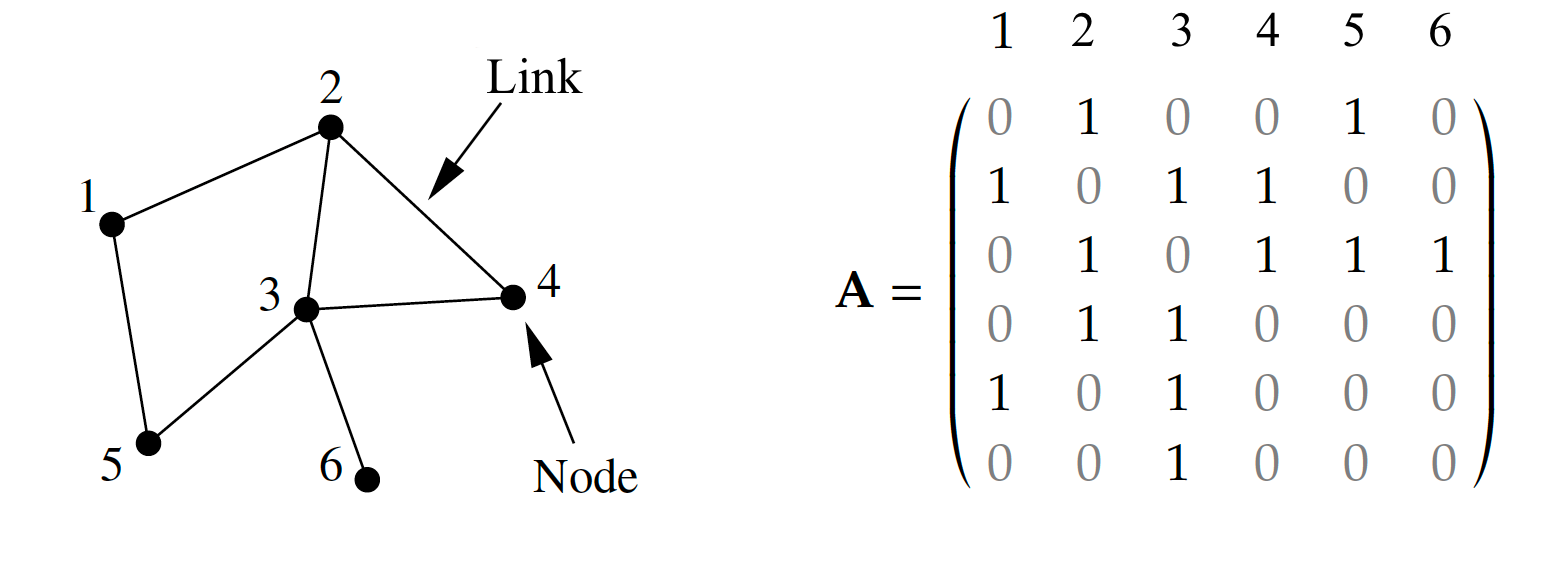
\includegraphics[width= 0.8\columnwidth]{figures/methods/fig_simpleNetwork.png}
    \caption[A simple graph]{A simple graph with its corresponding adjacency matrix. The diagonal elements must be zero for a network like this one with no self-edges, and the matrix must also be symmetric as every link between node $i$ and $j$ also exists between $j$ and $i$. Figure adapted from \cite{Newman2010}.}
    \label{fig:simpleNetwork}
\end{figure}

%Once presented with the formalism of graphs, we are ready to introduce the two most fundamental questions in network science: what does a node represent and when are two nodes connected? Trivial as they may seem, these questions are crucial to correctly describe a network according to a research question \cite{torres2021and}. In fact, networks are grouped in classes based on what their nodes represent --technological, transportation, economic, social, and biological/ecological \cite{Newman2010}. For our purposes, we will represent social and ecological systems as networks whose nodes are either agents of online social platforms (users and hashtags), species, or spatial locations in ecosystems. For example, in a food web, predator-prey interactions may be weighted to indicate the total energy flow between  predator and prey. Since, the energy flows from prey to predator, so a directed representation could also be used. In a social network, weighted connections may  represent the contact frequency between actors, and their sign may indicate friendship ($+$) or enmity ($-$). \\

Knowing which nodes are connected in a network provides, in principle, a comprehensive understanding of its structure. Nonetheless, interpreting raw network data can be challenging, which is why mathematical measures are defined to condense structural aspects quantitatively. Over the years, numerous measures have been defined. 
%including the degree $k$, the number of nodes connected to a node. 
In Appendix~\ref{chp:methods:predictors} we present a comprehensive list topological measures utilized in this thesis.

Finally, for the aim of this thesis, it is worth discussing bipartite networks. They are networks with two classes of nodes (or guilds in the ecological literature), and links connect only nodes of different classes. Bipartite networks commonly represent the membership of a set of species or people in groups of some kind. For example, we can represent pollination as a bipartite network in which the two guilds of nodes are plants and pollinators (regardless of taxa), and the links connect plants to their pollinators. To describe this mutualistic community, there is in principle no necessity for links that directly connect plants to other plants, or pollinators to other pollinators; the links in the bipartite network only run between nodes of different guilds. Therefore, if we group together all nodes of the same guild in the adjacency representation of the bipartite network, the diagonal blocks will be empty (Figure~\ref{chp:methods:fig:adjacencies}c).

\begin{figure}[t]
     \centering
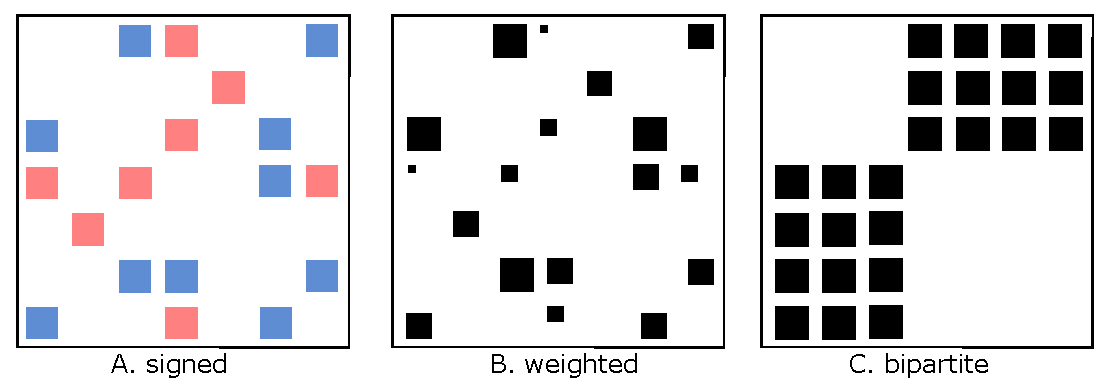
\includegraphics[width=\columnwidth]{figures/methods/fig_adjacencies.pdf}
 \caption[Adjacency matrices]{Adjacency matrices of several types of networks. Nodes are represented along the rows and columns. A square denotes the presence of an interaction, and its color and size represent the sign and weight, respectively. }
\label{chp:methods:fig:adjacencies}
\end{figure}

\subsection{Network models}

Network models suggest and explain the mechanisms behind node connection. All of these models have a similar approach: they eliminate unnecessary details and assume that links are set in a specific way. For example, just at random or according to some metrics. We may use models to reveal the circumstances in which our findings are valid and to understand the effects of the constraints that exist in the real world.

\paragraph{2D square lattice:} This model is not actually a \textit{complex} network, but a very ordered network since its nodes are discretely and consistently spaced from one another on the unit square. The eight adjacent nodes of a given node are thought to be their closest neighbors. The second closest nodes are the neighbors' neighbors, creating a total neighborhood of $24$ nodes.  This configuration can be thought of as a chessboard. The (discrete) distance between two nodes on a chessboard is the minimum number of moves that the king needs to move between them. In a more precise language, this definition of neighborhood is called Moore neighborhood and the distances between nodes are measured according to the Chebyshev distance. 2D lattices will be used in Chapter~\ref{chp:1} to represent a highly structured space.

\paragraph{Erd{\H{o}}s-R{\'e}nyi graph (ER):}  One of the most studied network models is the Erd{\H{o}}s-R{\'e}nyi  model \cite{erdos1959random}, where pairs of nodes are connected at random according to a fixed linkage probability $p$. It is used  as a null model in Chapters~\ref{chp:1} and \ref{chp:2} because it represents the simplest model for random graphs.

\paragraph{Random geometric graph (RGG):} 
In general, the random geometric graph is created by assigning a random location to its nodes by a predetermined probability distribution, and connecting two nodes by a link only if their distance falls within a predetermined distance, defined in a metric space \cite{Dall2002RandomGraphs}. For our purposes, nodes are randomly uniformly placed in the unit square and linked together according to the Euclidean distance.

\paragraph{Scale-free networks:} Our next step in complexity is to simulate scale-free networks. In particular, we employed the Barabasi-Albert model \cite{Albert2002StatisticalNetworks}. A network growth model based on preferential attachment where each new node is randomly connected to $m$ existing nodes with a probability proportional to the number of links that they already have.  To add up more realism, we use the Holme-Kim model \cite{Holme2002GrowingClustering}, which is a variant of a scale-free network and it can generate networks with a finite clustering coefficient. Both models are used in Chapter~\ref{chp:2}.

\paragraph{Network reshuffling:}
In the context of network theory, null models are
used to check whether a certain property of
a target network is just a consequence of chance, or
is due to a driving mechanism \cite{Newman2010}. The property can be
any macroscopic structure (e.g. nestedness in mutualistic
systems \cite{bastolla2009mutualism}), or a particular behavior of the underlying
dynamics (amplification of selection for advantageous mutants \cite{lieberman2005evolutionary}). The driving
mechanism to uncover can be the way in with the network is constructed (e.g. by an optimization process \cite{bastolla2009mutualism})
or the topological structure of the network (e.g. scale-free networks \cite{lieberman2005evolutionary}).\\

The modus operandi usually involves generating
randomizations of the original network where
some constraints are kept. Then, the property
will be evaluated in these networks and compared
against the original network.\\

We have already mentioned null models when presenting the ER
graph. This graph serves as a null model because it can
generate random networks with the same number of
nodes and average degree as the target network. If a
property of the original network does not depend on how
nodes connect, then the ensemble of ER networks, whose nodes
are linked at random, will also present that property. \\

Sometimes ER graphs are too disruptive
as null model since they dilute any trace of
structure. More conservative alternatives include
reshuffling the links and the weights of the original network. When reshuffling, links are interchanged among nodes
following certain rules. In particular, we
perform a reshuffling of each block
of bipartite networks in Section~\ref{chp:2:3:4}.
Those randomizations will be generated
through a Bernoulli process,
where a link between nodes $i$ and $j$ is created with probability
\begin{equation}
    P_{ij} = \frac{k_{i} + k_{j}}{2n},
\end{equation}
where $n$ is the total number of nodes, and $k_{i,j}$ is the degree of the original network.
This method conserves the connectance and the expected number of interactions of each node alone \cite{BiMat}. \\

Another reshuffling or rewiring is made in Section~\ref{chp3:1.3} as proposed in \cite{suweis2013emergence}, where links are interchanged according to a probability that depends on the degree and an external node property called \textit{niche}, which will be defined in Section~\ref{chp:methods:ecointeract}.

\section{Ecological networks}\label{chp:methods:econet}
\epigraph{Networks are particularly attractive to ecologists for providing a dynamic viewpoint from where scientists can simultaneously “see the forest and the trees”.}{\textit{Heleno et al.} \cite{heleno2014ecological}}
Once we have defined complex networks in general, we are ready to explore the role of networks in ecology. Depending on what nodes and links symbolize, we can divide ecological networks into two categories: interaction networks and spatial networks. %Nevertheless, this classification is highly biased toward the objective of this thesis. One could group networks across levels of organization, and would obtain a hierarchy of networks: individual-based networks, followed by species-based, and finally, clade-based networks \cite{guimaraes2020structure}.
One ecosystem may well be represented by these two categories simultaneously since a network is just a partial representation of one aspect of a complex system \cite{strogatz2001exploring}. Each type possesses attributes that make it suitable for dealing with certain questions.\\


%Chapter Structured interactions = space-based
%Chapter Structured predictors  and quantifiers = species-based

\subsection{Interaction networks}

Interaction networks are the most widely used networks in ecology \cite{kefi2020theoretical}. Nodes represent species and links are interactions between them. There are many well-documented types of interactions among species, so there are many types of networks depending on the interaction they describe. For instance, food webs are directed networks  of who eats whom, (Figure~\ref{chp:methods:fig:history}a). Ecological network research has been mainly focused  on food webs \cite{pascual2006ecological}, even if Darwin had already described the now-classic \textit{entangled bank} back in 1859, suggesting that species are ``dependent on each other in so complex a manner'' \cite{darwin1859origin}. There is a great variety of non-trophic interactions such as ecosystem engineering, facilitation, or antagonism \cite{kefi2012more}. Even more, there are interactions with  both trophic as well as non-trophic components, like pollination and seed dispersal.\\

\begin{figure}
    \centering
    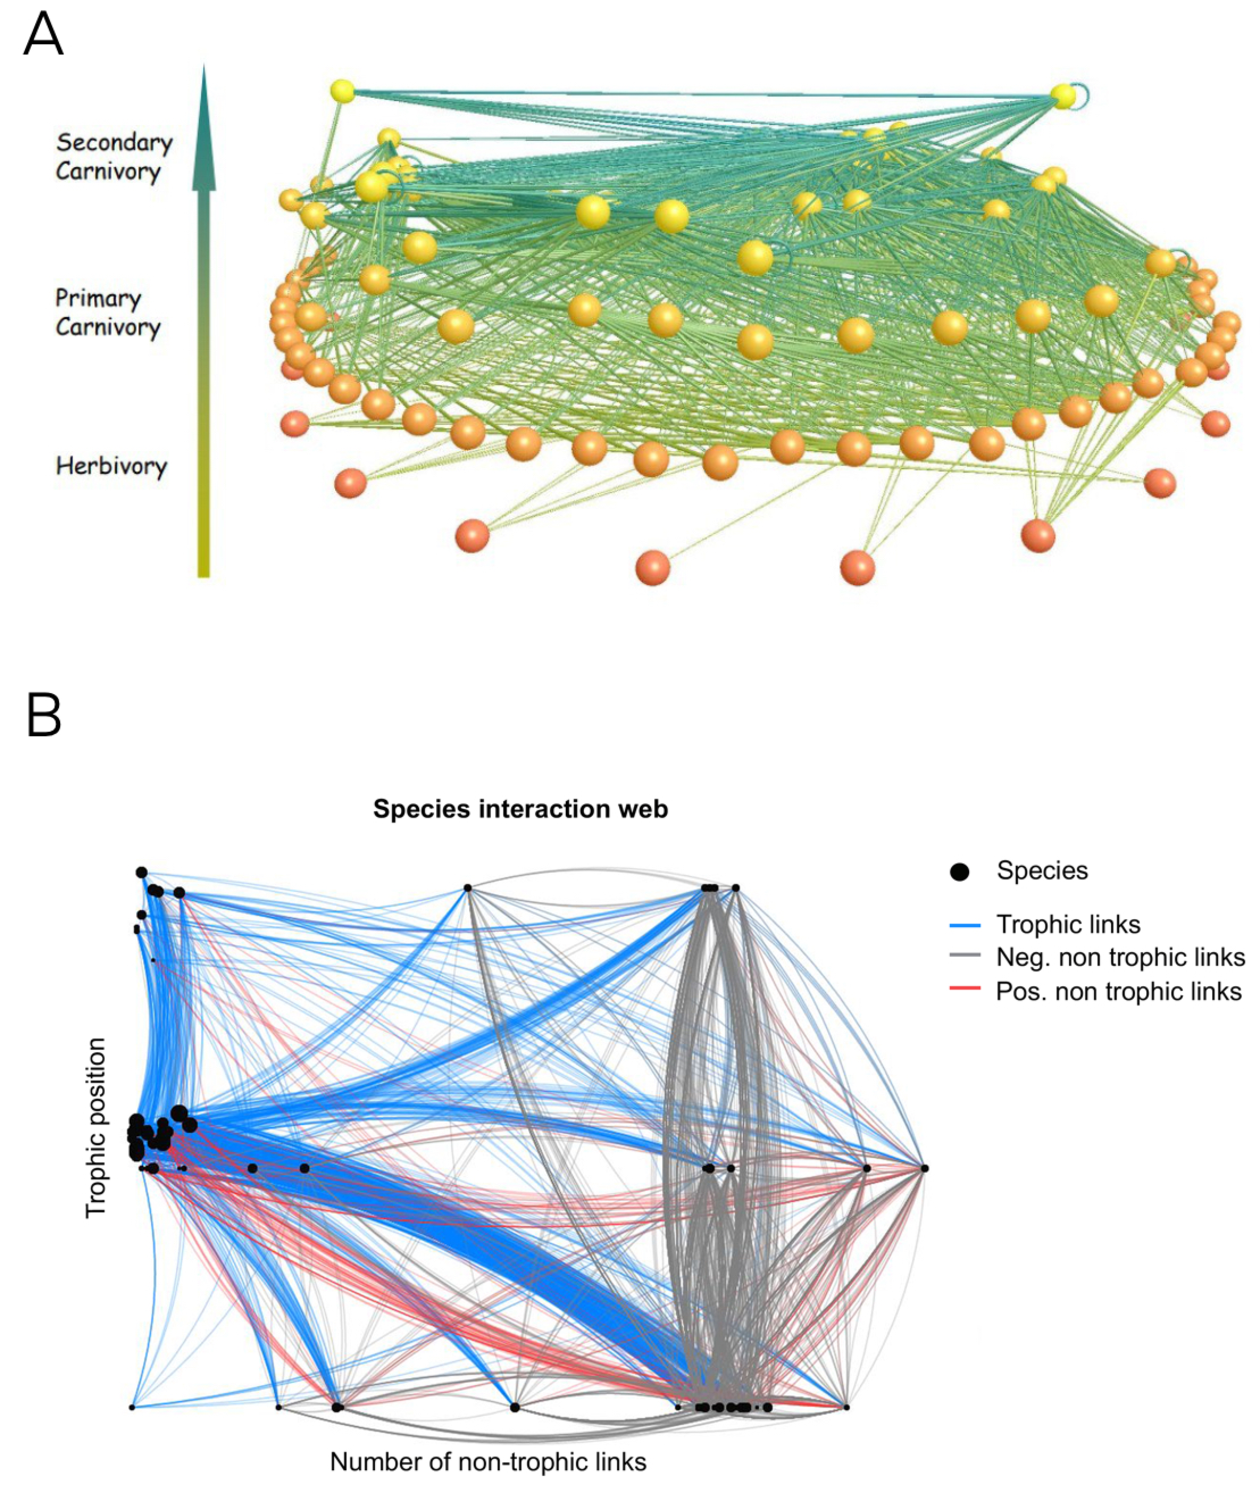
\includegraphics[width=0.8\columnwidth]{figures/methods/fig_history.pdf}
    \caption[Historical ecological networks]{(Panel a) The food Web of Little Rock Lake, Wisconsin \cite{martinez1991artifacts} was the largest food web in the primary literature for decades \cite{strogatz2001exploring}. Nodes are 181 functionally distinct \textit{trophic species} (11 fishes, 110 invertebrates, 59 autotrophs, 1 detritus). (Panel b) ``Network of trophic and non-trophic interactions between the 106 species of the Chilean web. Nodes indicate species and are sized by total degree. The vertical position is proportional to trophic level and the horizontal position is proportional to non-trophic degree. Edges are blue, red, and gray for trophic, positive, and negative interactions, respectively.'' \cite{kefi2016structured}}
    \label{chp:methods:fig:history}
\end{figure}

The sheer diversity of relations between species calls for a refinement of what interactions, and consequently links, are. More in general, one can think of two different pieces of information that can be called an interaction \cite{verhoef2010community}. First, an interaction may be a process, like the energy transfer from the resources to the consumers in food webs. In this case, they symbolize the interchange of something quantifiable like energy, nutrients, or biomass. And second, interactions may represent the \textit{effect} of a species on another. For example, if the growth of two species is enhanced when they coexist together, we deal with a positive-positive interaction. This type of interaction is called mutualism and can be generated by various processes. We have already mentioned pollination, which is a mechanism that gives rise to mutualistic interactions (Figure~\ref{chp:methods:fig:mut-comp}a). Another example is association resistance, in which a species obtains protection when it spatially associates with another species \cite{Dieckmann2000}. These mutualistic networks are described as undirected bipartite networks, sometimes weighed by the number of recorded visits for pollination or the number of co-occurrences for spatial association. The opposite effect is a negative-negative interaction, also termed competition. It can originate from trophic mechanisms, such as two predators sharing the same prey, as well as non-trophic mechanisms, like exploitative competition, when one species indirectly reduces another by  directly reducing shared resources \cite{wootton1994nature} (Figure~\ref{chp:methods:fig:mut-comp}b). \\
\begin{figure}[t]
     \centering
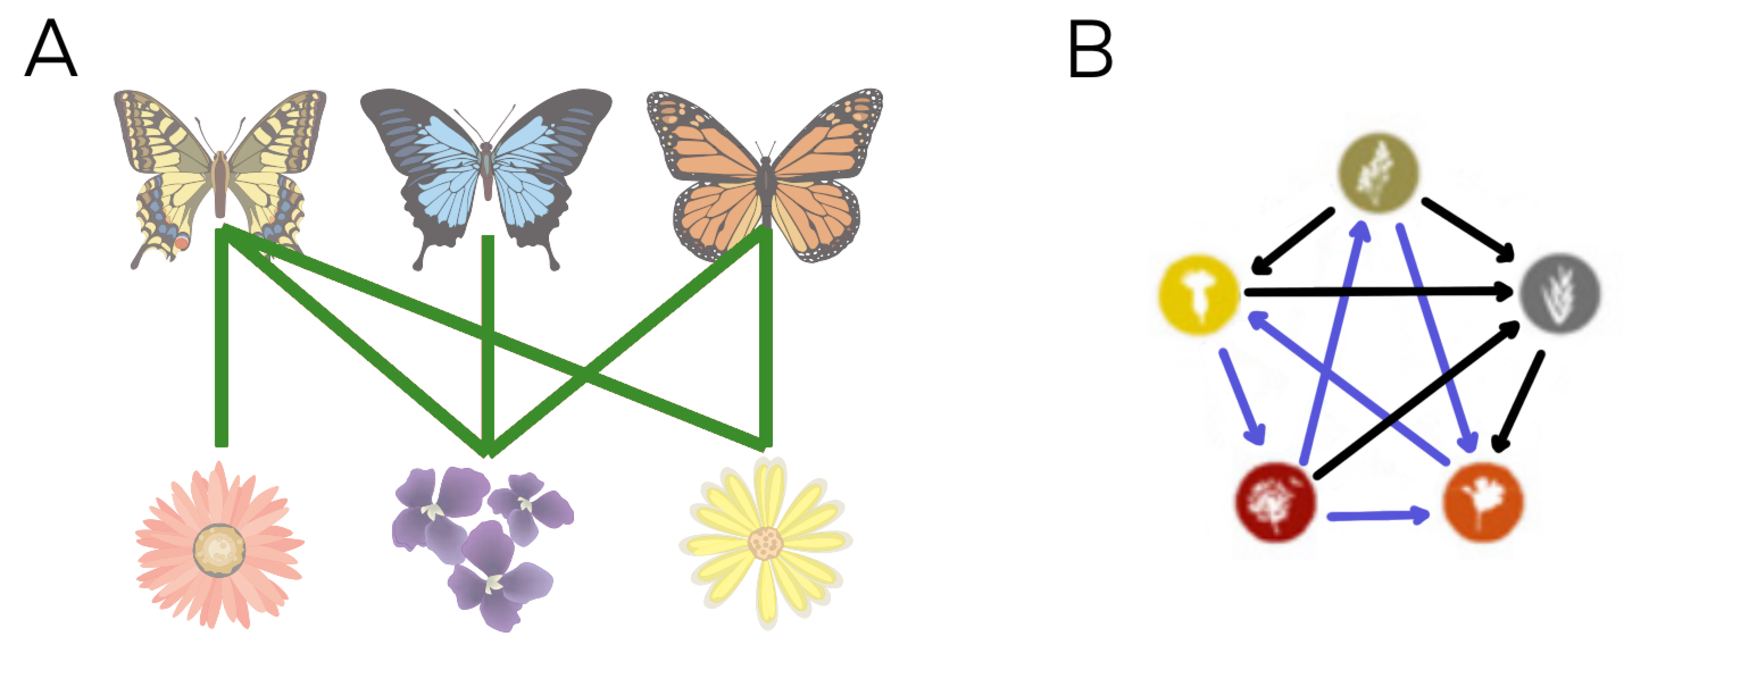
\includegraphics[width=\columnwidth]{figures/methods/fig_mut-comp.pdf}
 \caption[Mutualistic and competitive networks]{Two types of non-trophic interaction networks. (Panel a) Plant-pollinator mutualistic network. Note the bipartite division. Image extracted from \cite{rohr2014structural}. (Panel b) Competitive network. Directed links point from dominant species. Two intransitive cycles are shown in purple. Image adapted from \cite{soliveres2015intransitive}.}
\label{chp:methods:fig:mut-comp}
\end{figure}

Moreover, if several types of interactions are studied within the same representation, one can use signed networks (Figure~\ref{chp:methods:fig:history}b), or more complex structures, like multilayer networks \cite{pilosof2017multilayer} or hypergraphs \cite{golubski2016ecological}. \\

\subsection{Spatial networks}
Another type of ecological network revolves around space. In this case, nodes symbolize a location (a habitat, a patch) that can be inhabited by one or several individuals. Links represent the connections among the spatial locations. These connections can give rise to migrations, nutrient flows, or dispersal, and therefore networks may be directional and weighted. In Chapter~\ref{chp:1}, we will use a simple spatial network where nodes are spatial locations occupied by only one individual and links define seed dispersal pathways. \\

\begin{table}[t]
\centering
\caption{Types of ecological networks studied in this thesis}
\label{chp:methods:tab:networks}
\begin{tabularx}{1\textwidth}{ X X X X c}
\hline
\textbf{Network} & \textbf{Type}                                                                          & \textbf{Nodes}    & \textbf{Links}    & \textbf{Ch.}                              \\  
\hline
\hline
%Mutualistic      & \begin{tabular}[c]{@{}c@{}} bipartite\\ signed\\ (weighted)\end{tabular} & species           & interspecific non-trophic interactions & \ref{chp:2} \& \ref{chp:3}     \\
Spatial          & unsigned unweighted                      & spatial location & transfer of individuals (dispersal)    & \ref{chp:1}     \\
\hline
Mutualistic      &  bipartite signed (weighted) & species           & interspecific non-trophic interactions & \ref{chp:2} \& \ref{chp:3}     \\
\hline
Competitive      & signed (weighted)        & species           & interspecific non-trophic interactions & \ref{chp:2}  \& \ref{chp:3}     \\
\hline
Co-occurrence     & unsigned unweighted                        & individuals       & co-occurrence in the same location (overlap) & \ref{chp:3} \\
\hline
\end{tabularx}
\end{table}

\section{Ecological concepts}\label{chp:methods:ecointeract}
%%%%%%%%%%%%%%%%%%%%%%%%%%%%%%%%%%%%%%%%%%%%%%%%%%%%%%%%%%%%%%%%%%%%%%%%%%%%%%%%%%%%%%%%%%%%%%%%%%%%%%%%%%%%%

 Interactions are what connect species. They are then a central factor that drives community dynamics, one of the main subjects in ecological research. Along this thesis, we take the approach of studying the effects of ecological interactions by a parametric, or model-driven approach. We can describe these effects as a system of first-order, ordinary differential equations, i.e. equations containing functions of one or more independent variables (abundances $N_i$ or frequencies of species) and their first derivative with respect to time. We can write a general form of these systems as:
 \begin{equation}
     \frac{dN_i}{dt} = N_i f_i(N_1,... , N_S)
 \end{equation}


 In this Section, two theoretical frameworks broadly used in population and evolutionary dynamics are presented: the generalized Lotka-Volterra equations and the replicator equation. Then, we go one step further and explain a dynamical model --the niche model-- which incorporates a network construction algorithm. Finally, we discuss how a certain configuration of competitive strengths can modify the coexistence and stability of a community.

\subsection{Generalized Lotka-Volterra equations}\label{chp:methods:LV}

%The Lotka-Volterra equations were first proposed as a simple model of predation to explain the oscillatory behavior of certain fish catches in the Adriatic \cite{murray2002mathematical}. They have been quite helpful in raising relevant questions since they are able to be analytically tractable and present interesting dynamics. In fact, they were quickly generalized to include more realistic constraints and other types of interactions and to involve more than two species. \\

The generalized Lotka-Volterra model (GLV) is one of the simplest and most used nonlinear model for population dynamics of multiple interacting species. It is also a mathematical paradigm --in the sense that other models can be transformed into GLV form \cite{page2002unifying}. We can write a compact formulation of the model as:
\begin{equation}
    \frac{\textbf{dN}}{dt} = D(\textbf{N}(t))(\rho + A \textbf{N}(t))
\end{equation}
where $\textbf{N}(t)$ is the column vector of length $S$ (the total number of species) that contains the abundances of all species at time $t$, $\rho$ is the vector of intrinsic growth rates, $A$ denotes an $S \times S$ matrix of interaction coefficients, and $D(\textbf{N})$ is a diagonal matrix with the $N_i$ as diagonal elements. The intrinsic growth rates measure the growth (or decline if they are negative) of a species when it is in isolation. \\

With this representation, some important features of the community can be studied, like coexistence and stability. If $A$ is invertible, we can look for a feasible equilibrium, i.e. a solution of the equation $\rho + A\textbf{N} = 0$, where all species have positive abundances.  The stability of the stationary points can be studied through the eigenvalues of $A$. %However, since the number of parameters of the GLV grows with the number of species involved, if we choose their values at random, the community will probably collapse into smaller systems because of extinctions.\\

Regarding the possible types of dynamics, the Lotka-Volterra equations have been thoroughly studied for $2$ species, where fixed points, limit cycles around the equilibrium, and unbounded growth can appear depending on the signs and values of the elements in $A$ \cite{murray2002mathematical} 
 (Figure~\ref{fig:LV}a). When we study multi-species systems, more exotic behavior like chaos can appear \cite{houfbauer1998book} (Figure~\ref{fig:LV}b).\\ 

\begin{figure}[t]
    \centering    
    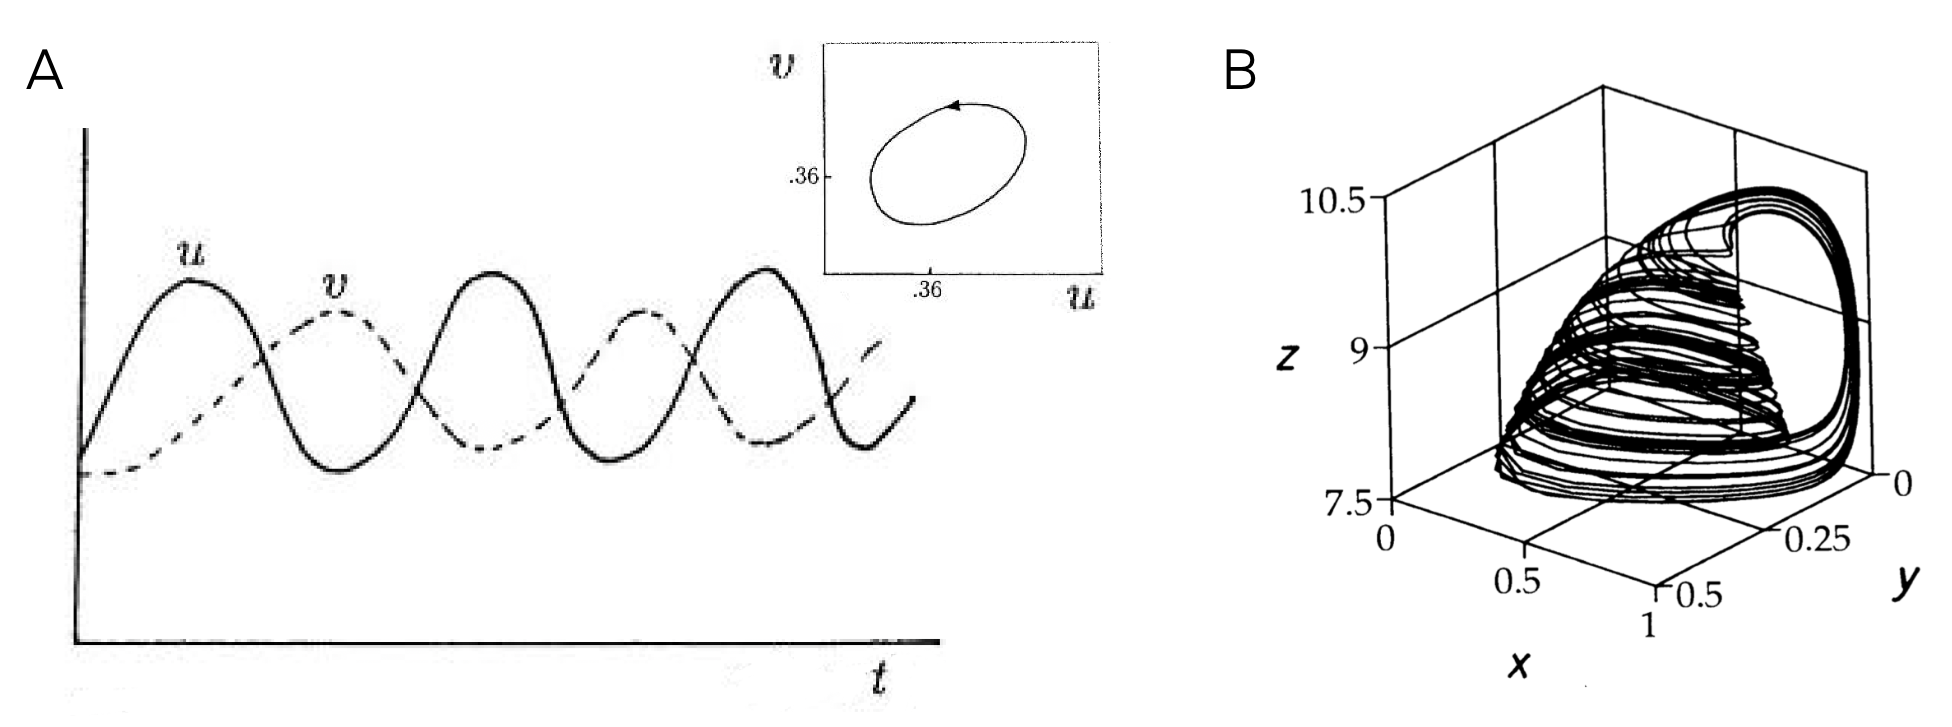
\includegraphics[width=\columnwidth]{figures/methods/fig_LV.png}
    \caption[Historical example of Lotka-Volterra equations]{The Lotka-Volterra equations were first proposed as a simple model of predation to explain the oscillatory behavior of certain fish catches in the Adriatic \cite{murray2002mathematical}. In (Panel a), we find the periodic solution for the original Lotka-Volterra equations, which only involve two species: a predator-prey system. The phase trajectory of the limit cycle is in the inset. Figure from \cite{murray2002mathematical}. These equations have been quite helpful in raising relevant questions since they can be analytically tractable and present interesting dynamics. In fact, they were quickly generalized to include more realistic constraints, other types of interactions, and to involve more than two species. For example, one can get chaos from 3 species with trophic relations. The attractor of such a system is depicted in (Panel b), from \cite{hastings1991chaos}. }
    \label{fig:LV}
\end{figure}

Within this approach, we can classify the interactions as follows: two species are in a predator-prey relationship when one population declines while the other increases, competition exists if the growth of both species decreases, and mutualism or symbiosis is the term used when both populations increase from the presence of each other. These situations are visible in the interaction matrix $A$. If, for example, two species $i$ and $j$ compete, both $A_{ij}$ and $A_{ji}$ will be negative. However, when studying different types of interactions in the same community, it is more convenient to create distinct interaction matrices for each type. Since we will study a system with mutualism and competition in Chapter~\ref{chp:3}, let's exemplify how the GLV of such a system would look by introducing a model describing the dynamics of a plant-animal community:
\begin{equation}
\label{eq:LVcm}
{\begin{aligned}{\frac {dP_i}{dt}}&=P_i \left(\rho_i^P - \sum_j \beta_{ij}^{P}P_j + \sum_k \gamma_{ik}^{P} A_k \right) \\[6pt]
{\frac {dA_k}{dt}}&=A_k \left(\rho_k^A - \sum_l \beta_{kl}^{A}A_l + \sum_i \gamma_{ki}^{A} P_i \right),
\end{aligned}}
\end{equation}
where $P_i$ and $A_k$ are the variables for the abundances of plant and animal species. The new parameters correspond to the matrices describing intra-guild competition $\beta$ and the mutualistic interactions $\gamma$. Examining the mutualistic benefit, we see that its effect gets stronger with larger species abundance. However, the effect is far from linear, as is supposed in the previous equation. A typical assumption is a mutualistic response that saturates \cite{bastolla2009mutualism,rohr2014structural, suweis2013emergence}:
\begin{equation}
\label{eq:LVcmholling}
{\begin{aligned}{\frac {dP_i}{dt}}&=P_i \left(\rho_i^P - \sum_j \beta_{ij}^{P}P_j + \frac{\sum_k \gamma_{ik}^{P}A_k }{1+ h \sum_l \gamma_{il}^{P} A_l} \right) \\[6pt]
{\frac {dA_k}{dt}}&=A_k \left(\rho_k^A - \sum_l \beta_{kl}^{A}A_l + \frac{\sum_i \gamma_{ki}^{A}P_i }{1+ h \sum_j \gamma_{kl}^{A} P_j}\right).
\end{aligned}}
\end{equation}
The fraction in these modified Lotka-Volterra equations is called Holling Type-II functional response and imposes a limit to the mutualistic effect by adding a handling time $h$. This restriction considers that species are unable to engage with a high number of mutualistic partners because each interaction involves time. With this functional response, the benefit from mutualistic interactions does not increase monotonically as the number of species increases, bounding the dynamics.
%A typical derivation of Type-II response assumes that handling a ''unit'' of consumer prey takes Th time, with Ts time spent searching and Tt total time, giving: Tt = Ts + ThY with the amount of prey caught Y .
%less prey = limitation is the finding factor.
%lots of prey = saturation = limiting is h.




%%%%%%%%%%%%%%%%%%%%%%%%%%%%%%%%%%%%%%%%%%%%%%%%%%%%%%%%%%%%%%%%%%%%%%%%%%%%%%%%%%%%%%%%%%%%%%%%%%%%%%%%%%%%%
\subsection{Replicator dynamics}\label{chp:methods:repli}
 The replicator equation is a well-known equation in evolutionary game theory \cite{houfbauer1998book}. It assumes that the strategies of the game --actions that rational players choose to play-- are selected according to their frequency $x_i$. The equation sets how the evolution of these frequencies, $\dot{x_i}$, varies according to its rate of success. We will use the replicator dynamics in Chapter~\ref{chp:2} to model species frequencies instead of strategies, so we will continue the description of the dynamics with $n$ species in mind rather than strategies. \\
 
The replicator equation captures the intuitive idea that species that do well grow faster. To quantify how well a species is doing, the local fitness of a species, $f_i$, is used. Fitness is a broad concept with several definitions depending on the context. Here, it is just a linear combination of the species frequencies given by payoffs $a_{ij}$ that account for the reproductive success:
\begin{equation}
    f_i = \sum_{j = 1}^{n}  a_{ij} x_j.
\end{equation}\label{eq:localfitness}
 Thus, the replicator equation is a phenomenological description of the system. It only tells us that the fitness of species $i$ will increase by $a_{ij} x_j$ if the interaction occurs, but it does not take into account how species $i$ and $j$ interact. \\
 
 More precisely, $x_i$ varies according to the difference between its local fitness and the average fitness of the population,  $ \phi = \sum_{j} x_j f_j = \sum_{j,k} x_j a_{jk} x_k$, and the evolution equation reads
 \begin{equation}
    \dot{x_i} = x_i \left( \sum_j a_{ij} x_j - \sum_{j,k} x_j a_{jk} x_k \right),
    \label{chp:methods:eq:replicator}
\end{equation}
 where $(a_{ij})$ is the so-called payoff matrix. Species $i$ will grow if the first term inside the parentheses is greater than the average fitness of the community of $n$ species. In this context, we can interpret fitness as how well a species will grow according to its interactions. \\
 
 Regarding the possible solutions, they are all confined in the $(n-1)$-simplex, the set of non-negative points $(x_1, ..., x_n)$ whose coordinates are all non-negative and add up to one. This is simply a consequence
 of working with the frequencies of the species, which have the property $\sum^n_{i = 1} x_i = 1$.
For the case of two species, at most one isolated equilibrium where $x_i > 0, \, \forall i$ (i.e. in which no species going extinct) can be reached \cite{Nowak2006EvolutionaryDynamics}. As the number of species increases, more exotic behavior can occur. For example, if $n \geq 4$, the possibility of chaos appears. Moreover, the replicator equation is mathematically equivalent to the Lotka-Volterra equations \cite[Chapter~7]{houfbauer1998book}, so whatever outcome is true for one equation will hold for the other\cite{page2002unifying}.\\
 
During this thesis, we will consider the replicator dynamics on a graph, where each node is occupied by a different species. The payoff matrix elements $a_{ij}$ are now zero if species $i$ does not interact with species $j$, and  equals an interaction strength value $\alpha_s$  otherwise. The diagonal terms are fixed to $c < 0$, since the effect a species has on itself is usually regulatory. In the extreme case where none of the species interact with each other ($a_{ij} = 0 \forall i,j$), the local fitness equals the average fitness, and the system remains in its initial condition. In the all-to-all case (when every species interacts with every other species), the $n$ species coexist with density $x_i = 1/n$. Other configurations yield different solutions, usually involving the extinction of several species. Their full analysis will be carried out in Chapter~\ref{chp:2}.
%%%%%%%%%%%%%%%%%%%%%%%%%%%%%%%%%%%%%%%%%%%%%%%%%%%%%%%%%%%%%%%%%%%%%%%%%%%%%%%%%%%%%%%%%%%%%%%%%%%%%%%%%%%%%%%%%%%%%%%%%%%%%%%%%%%%%%%%%%%%%%%%%%%%
\subsection{Niche theory and beyond}\label{chp:methods:niche}
Since the presence of ecological (and evolutionary) processes is encoded in the network, we ask about the mechanisms that give rise to the observed network structure. Some basic models may produce communities with realistic topologies. One such approach is the niche model \cite{cai2021niches}. Its main idea is that species choose their interaction partners to maximize their abundance.\\

The niche model incorporates the elusive concept of niche, and adaptive species connection dynamics. The niche is interpreted here in line with Hutchinson's fundamental niche: the hypervolume defined by the limiting factors of the species growth \cite{hutchinson1957concluding}. These include the environmental conditions that allow species to satisfy their minimum requirements, so that the death rate of a local population is equal to or smaller than the birth rate \cite{chase2009niches}. \\

The idea of using niches to infer network structure was initially developed for food webs \cite{williams2000niche}, and it has been recently adapted to mutualistic communities \cite{cai2021niches}. We will introduce the model in this latter context, through a pollinating community with two guilds: plant species $P$ and pollinators $A$, where there is competition inside guilds and mutualism across guilds. \\

The key aspect of the model is that every species is randomly assigned a \textit{niche profile}, which is a region on the abstract one-dimensional niche axis $s$. The niche axis represents the operating or living range of the species and is shared by all species within a guild. The region can be defined in several ways, like an interval (typically in food webs), or a Gaussian function. We will continue the presentation of the model with a Gaussian function for illustrative purposes, but in Chapter~\ref{chp:3} cosine similarity will be used.  Hence the niche profile is a statistical distribution of the resources used by a given species. We define \textit{niche overlap} as the overlapping between niche profiles of two species. For within-guild overlaps, is given by:
\begin{equation}
    G^{PP}_{i j}  =  \int G_i^P(s) G_j^P(s) ds,
\end{equation}
 where $ G_i^P(s)$ is the Gaussian profile of plant species $i$. The overlap quantifies the niche similarity of species and is a proxy for competition within the guild. Species with highly overlapping niches are thought to compete for the same set of limited resources, for example, resources related to habitat conditions like soil pH or similar nesting sites. For cross-guild overlaps, we get:
\begin{equation}
    G^{PA}_{ik}  =  \int G_i^P(s) G_k^A(s) ds.
\end{equation}
In this context, the overlap captures the niche complementarity of mutualistic partners. This is based on the assumption that both partners must live in the same environment for the mutualistic relationship to occur. For example, pollinators must be fully developed when the flower is functional, i.e. close physical proximity between the organisms is required.\\

Then, it is assumed that species abundances evolve following some dynamics and, as mentioned earlier, that species can adapt their connections. In our version of the model developed in \cite{palazzi2021ecological}, the driver behind the adaptation is the maximization of abundance.  Niche overlap comes into play here because it is coupled with the strength of the interactions. Higher overlap leads to more intense interactions. The model develops as follows: a randomly selected species tries to connect to a different mutualistic partner, removing one of its previous links. If the abundance of the species rises, the rewiring is accepted; otherwise, it is rejected (Figure~\ref{fig:nicheModel}b).  To reflect the fact that it is harder to remove links from a specialist than from a generalist species, the rewiring probability of a species is proportional to $p_{PA} \propto 1 - k_{P}^{-1}$. Between rewiring attempts, we wait until the population dynamics has reached an equilibrium. \\

The number of species and the connectance of the networks of interactions (which are conserved through the optimization process) can be empirical values. In this way, the model can reproduce key patterns in food webs as the fractions of species at the top, intermediate, and basal
trophic levels \cite{williams2000niche}, or to explain the emergence of patterns of nestedness and in-block nestedness \cite{suweis2013emergence,cai2021niches} in mutualistic networks (Figure~\ref{fig:nicheModel}a). In Chapter~\ref{chp:3}, we will apply the model to a non-biological system, the user-hashtag partnerships, because mutual benefits exist in this context too.
 \begin{figure}[t]
 \centering
   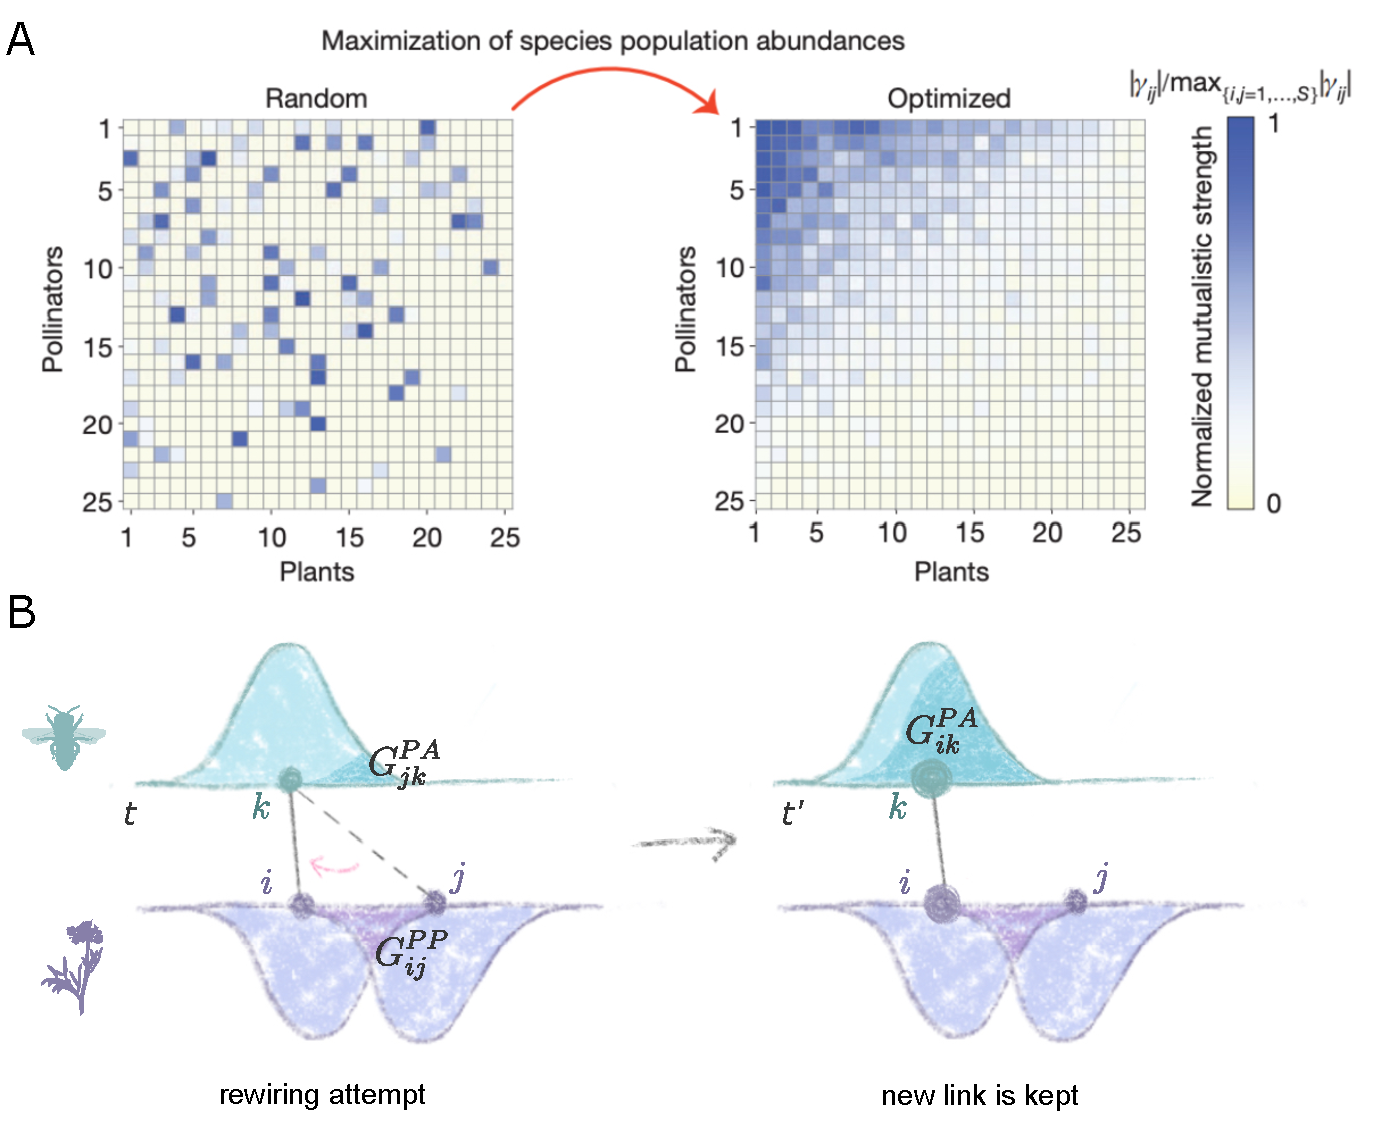
\includegraphics[width=\columnwidth]{figures/methods/niche.pdf}
    \caption[ Schematic representation of the niche model]{(Panel a) Abundance optimization leads to nested networks in ecological communities. Figure from \cite{suweis2013emergence}. (Panel b) Schematic representation of the niche overlaps and rewiring. In the example, node size symbolizes abundance and darker areas are niche overlaps. A pollinator $k$ rewires to a new partner flower $i$ with higher niche overlap ($G^{PA}_{ik} > G^{PA}_{jk}$). Since the abundance of the pollinator rises, the new link (solid line) is accepted. Images of pollinator and plant are available under CC0 $1.0$  license.}
   \label{fig:nicheModel}
\end{figure}
%Images of pollinator $Megachile\, Rotundata$ and plant $Crithmum\, maritimum$ available under CC0 $1.0$  license.
%%%%%%%%%%%%%%%%%%%%%%%%%%%%%%%%%%%%%%%%%%%%%%%%%%%%%%%%%%%%%%%%%%%%%%%%%%%%%%%%%%%%%%%%%%%%%%%%%%%%%%%%%%%%%%%%%%%%%%%%%%%%%%%
\subsection{Intransitivity}\label{chp:methods:intra}
\epigraph{… by chasing your victim faster, you actually help out the guy who’s chasing you.}{\textit{Kerr et al.} \cite{kerr2002local}}
Competition plays a vital role in the evolution and maintenance of ecosystems. In fact, one of the long-standing questions in ecology is why there are so many species despite competition. A possible solution that has been proposed is making competition --a negative interaction often related to struggle and hassle-- work for biodiversity. But not all sorts of competition are useful to promote coexistence. In particular, researchers have considered a concrete arrangement of competitive interactions that is not hierarchical: intransitive interactions \cite{soliveres2018everything}. \\

When a community presents a hierarchical competitive structure, species could be sorted according to how well they outcompete each other. When competing for the same set of resources and with no other mechanisms at play, we would eventually find that the species with the highest ranking would have total predominance. All the others would become extinct since they perform worse. This situation is called the principle of competitive exclusion. On the other hand, with non-hierarchical interactions, if species $A$ outcompetes species $B$ and $B$ outcompetes species $C$, then species $C$ outcompetes species $A$. In such circumstances, there are no clear weak species. The abundance of the different species will cycle \cite{may1975nonlinear}, preventing one single species from taking over the whole population.  A well-known example of such cycles is the rock-paper-scissors game (Figure~\ref{chp:methods:fig:RPS}).  \\

\begin{figure}[t]
     \centering
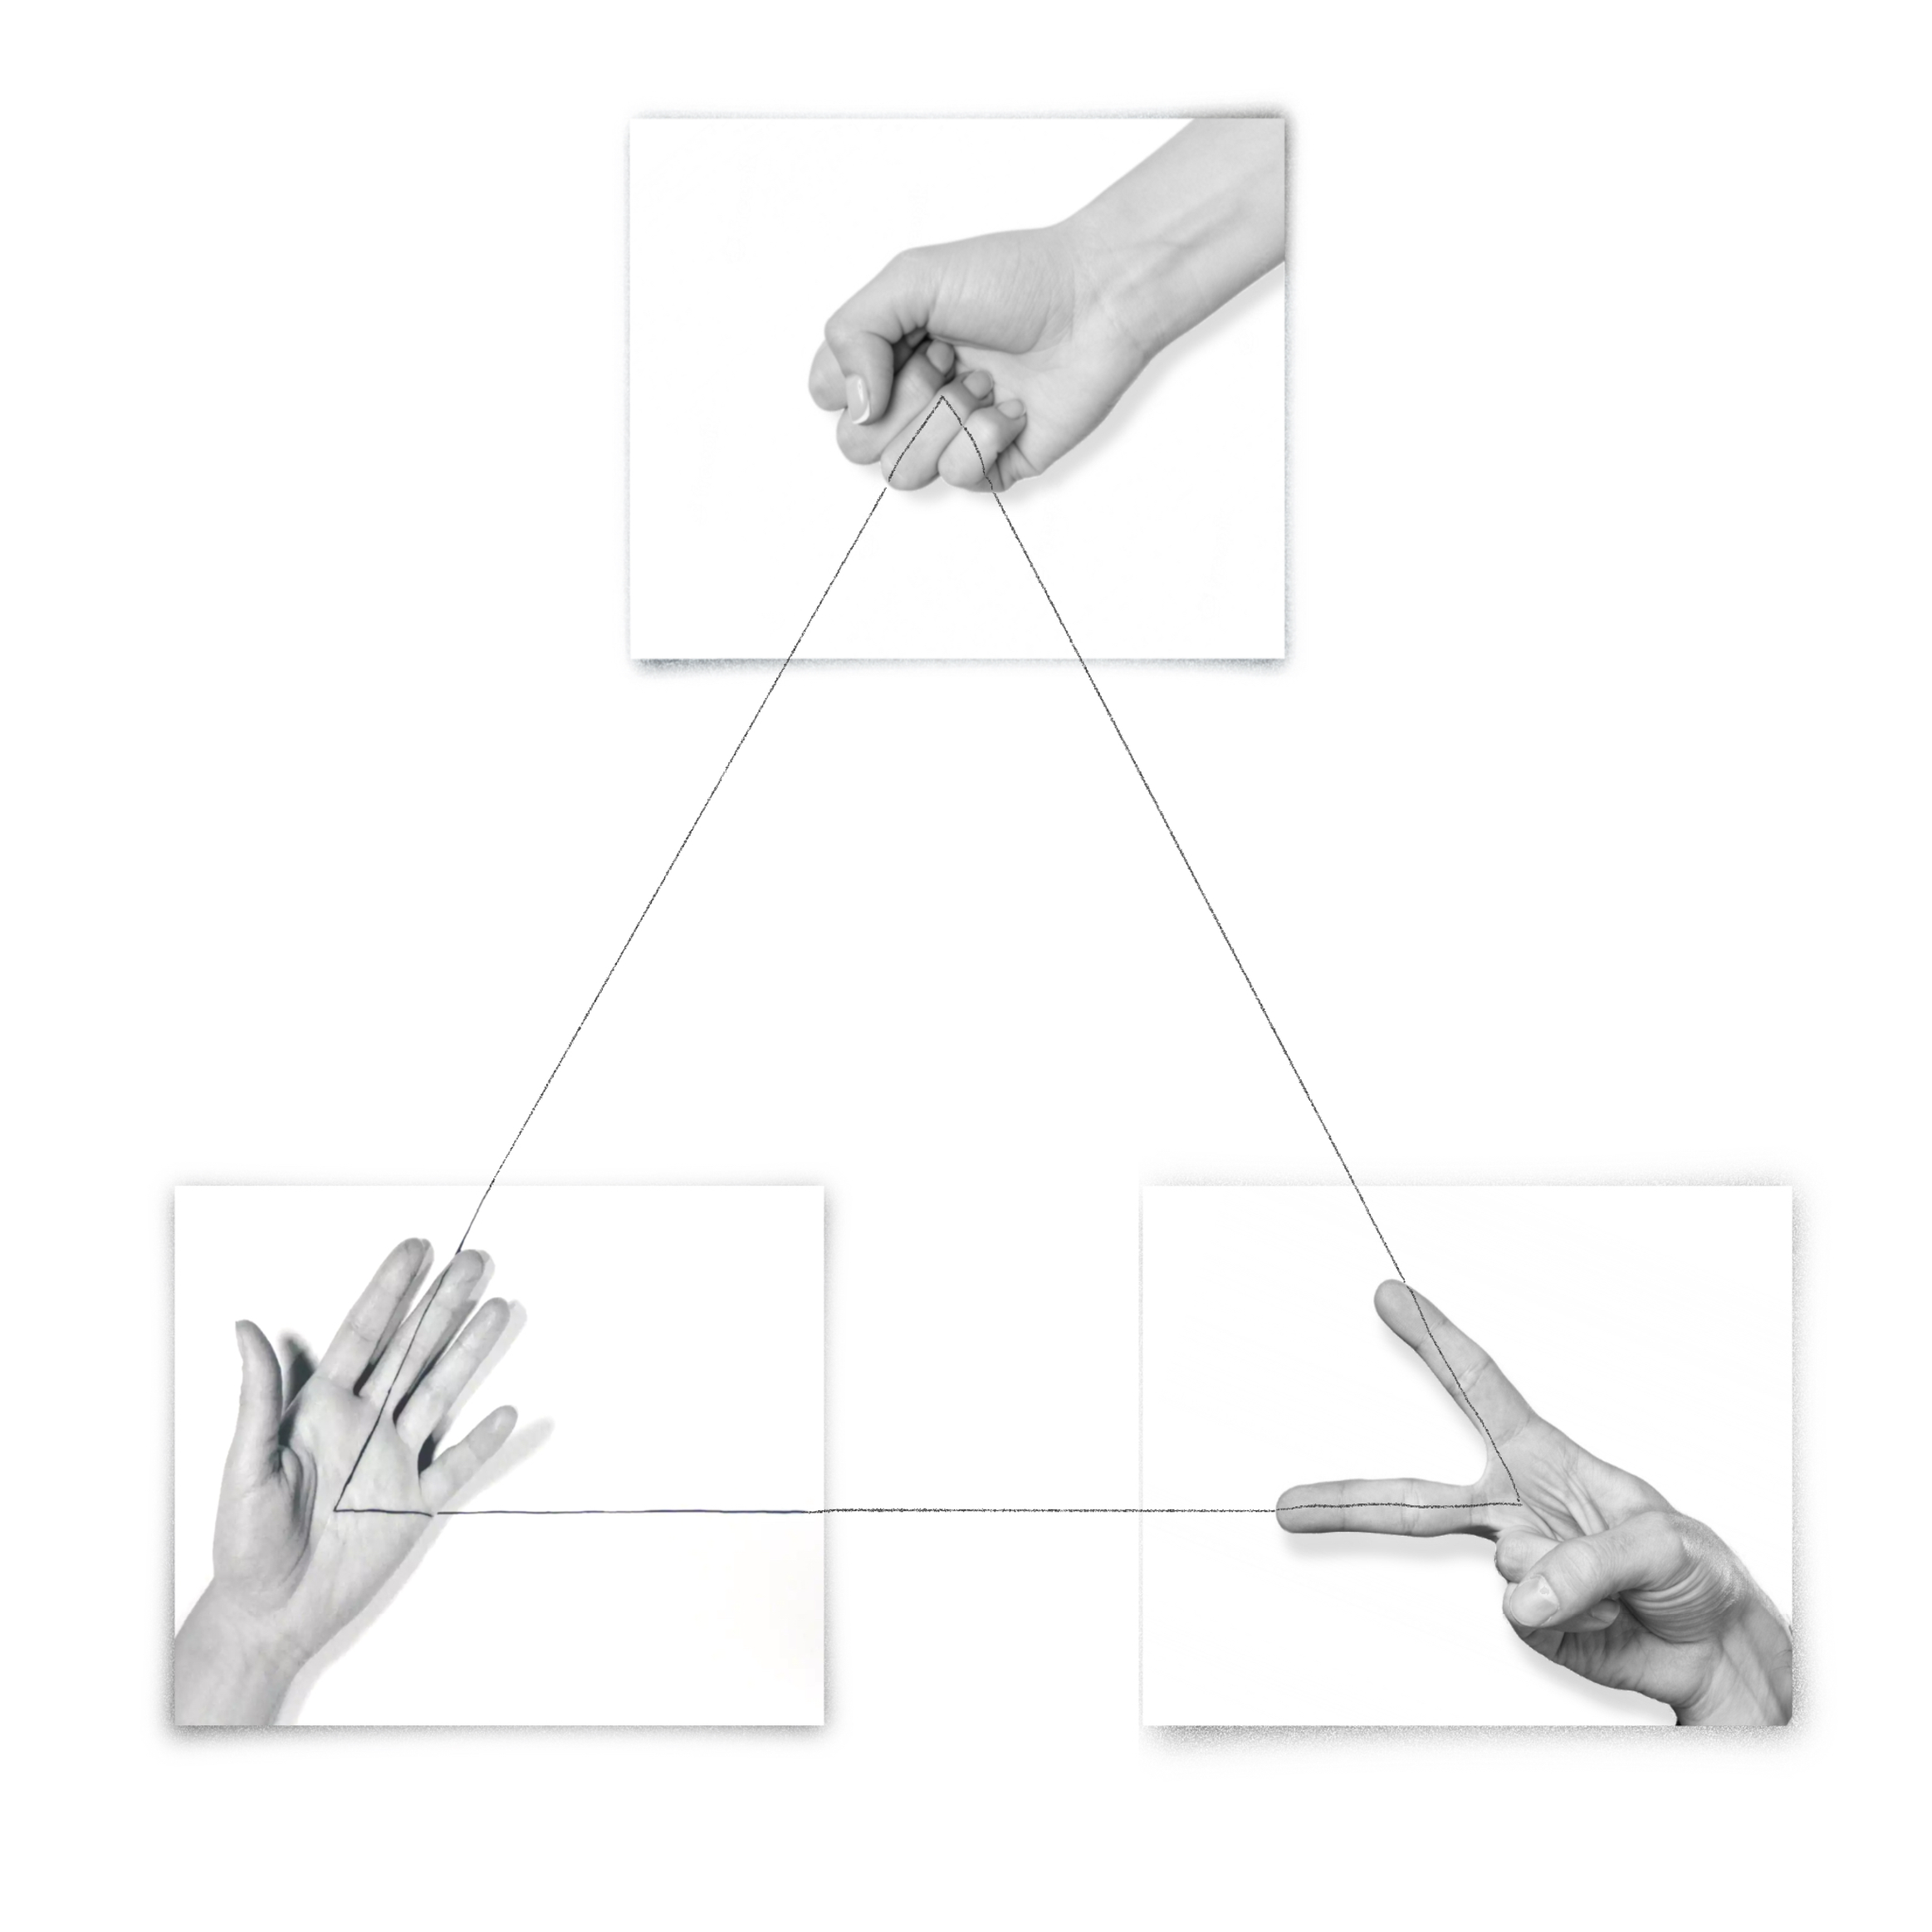
\includegraphics[width=0.7\columnwidth]{figures/methods/fig_RPS.pdf}
 \caption[Intransitivity diagram]{In the common playground game, rock crushes scissors, scissors cuts paper, and paper covers rock. No strategy has an advantage, there is no hierarchy, and because of this, multiple species may coexist by cycling in and out of dominance. Image inspired on Liliana Porter's wall installation ``Untitled (triangle)'' (1973).}
\label{chp:methods:fig:RPS}
\end{figure}

 There are some classic examples of intransitivity in natural systems, such as the side-blotched lizards \cite{sinervo1996rock}. The male lizards use, depending on their throat color, three different mating strategies that form an intransitive cycle, creating oscillations in color dominance over the years. Another seminal work is the one conducted on \textit{E. coli} by Kerr \textit{et al.} \cite{kerr2002local}, where three strains regulate the resistance, sensitivity, and production of a toxin. In theory, they form an intransitive cycle, but coexistence only actually occurs if their movement is constrained in a Petri dish. However, these behaviors, which can easily arise in simple mathematical models of $3$ or more species \cite{may1975nonlinear}, have proven in general to be difficult to find in nature \cite{godoy2017intransitivity, friedman2017community}.\\

%Despite these works suggesting that intransitivity is hard to find, a species cannot be great at everything. This opens a door to intransitive effects, and all that remains is where to find them. 
A possibility is to abandon small communities --3 lizards, 3 bacteria-- and study systems with a larger number of organisms. The reason lies in the simple, but not for that less powerful idea that biodiversity begets biodiversity \cite{maynard2017diversity}. If the number of species in a community is high, it is likely that they had very different competitive strategies and evolutionary histories. More species open the possibility of more potential and realized interactions. In this case, intransitive interactions can form, creating a self-reinforcing protection against competitive exclusion. Furthermore, recent studies have paired intransitive interactions with auxiliary mechanisms, such as spatial constraints \cite{Laird2015} or mobility \cite{reichenbach2007mobility}, to obtain stable systems. In Chapter~\ref{chp:1}, we will investigate how the locality of interactions affects the dynamics of intransitive communities.\\

%In fact, plant communities are species-rich assemblages where intransitive interactions have been empirically found. Intransitive competition occurred in more than $65\%$ of the sites in a study involving drylands and agricultural grasslands \cite{soliveres2015intransitive} and was associated with higher biodiversity. However, another empirical work found that intransitivity was uncommon in annual plant communities \cite{godoy2017intransitivity}. \\

%The dearth  (for now) of empirical data has not stopped researchers from developing more advanced computational models. Their main characteristic is that intransitivity is paired with auxiliary mechanisms not only to violate the principle of competitive exclusion, but also to get rid of oscillations and obtain a stable system. After all, oscillations in discrete systems may end up in extinctions if they are wide enough \cite{may1975nonlinear}. In another theoretical work, intransitive cycles are combined with mobility, obtaining a critical threshold below which mobility sustains species diversity \cite{reichenbach2007mobility}.
%According to the works in these lines,  a number of requirements should be met in order for intransitive communities to emerge and persist \cite{permogorskiy2015competitive}. As a summary:
%\begin{enumerate}
%    \item The system has a potential appropriate diversity. Too small systems stagnate and die out by cascades of extinctions.
%    \item The interactions take place in a relatively limited stable space. External disturbances are minimal.
%    \item The development of competitive abilities carries a cost. There are trade-offs.
%\end{enumerate}
%HOI or mobility are just some examples of intransitivity's companions that emphasize the importance of taking other factors into account when disentangling the bank. 

%Summing up, theoretical models suggest that intransitive competition plays a significant role in promoting species coexistence, although there is currently insufficient empirical data to draw any firm conclusions. In fact, whether intransitivity is common or rare in nature and its importance in real ecosystems is still an open question.
%%%%%%%%%%%%%%%%%%%%%%%%%%%%%%%%%%%%%%%%%%%%%%%%%%%%%%%%%%%%%%%%%%%%%%%%%%%%%%%%%%%%%%%%%%%%%%%%%%%%%%%%%%%%%
\subsection{Macroecological patterns}\label{chp:methods:macro}
Observing nature as Darwin and Wallace did is just the first step to truly understanding its complexity. As a next step, ecologists have traditionally had a hypothetico-deductive, often experimental approach, where a small and defined part of an ecosystem was taken apart to study how it works. This reductionism, whose success should not be discounted, has a particularly important limitation in ecology:  the results of microscopic studies cannot easily be extrapolated to larger scales, hindering a complete synthesis of the understanding of the structure and dynamics of ecosystems. A lot of replications should be made in different habitats and latitudes, and there are simply not enough resources to carry them, making it difficult to place results in a broader perspective. \\

A complementary step is to keep track of what is observed to analyze the patterns and behaviors that emerge. This is the essence of macroecology, an approach that focuses on patterns and relationships at large spatial and temporal scales \cite{brown1995macroecology}. It emphasizes the study of biodiversity and ecological processes across different geographic regions. The goal of macroecology is to identify and understand the broad-scale ecological patterns –macropatterns– and processes that shape the distribution and abundance of species and ecosystems. Certain universal rules have been discovered \cite{verberk2011explaining}, such as the fact that larger habitats tend to have more species than smaller ones. Additionally, it is almost always the case that in any community of species, there are a few species that are very abundant and many more that are rare. \\

One of the key patterns in macroecology is the species-area curve, which describes the relationship between the size of a geographic area and the number of species that can be found within it. This relationship is often depicted by plotting the number of species observed in a sampled area against the size of that area. The species-area curve typically follows truncated scale-free behavior, which means that the number of species increases rapidly with the area at first, but then levels off as the area becomes very large. \\

Macroecological research not only offers greater potential for generality but also presents a powerful tool for prediction. Patterns have been used from estimating the total number of species on Earth \cite{mora2011many} to predict how many species are likely to be lost as a result of habitat destruction and other human activities. For example, faced with this latter problem, researchers in exploit data on the species-area curve of the fauna of isolated mountain ranges to predict the species that would go extinct under climate warming, without detailed knowledge of their population biology \cite{mcdonald1992using} (Figure~\ref{chp:methods:fig:exmacro}).\\

\begin{figure}[t]
     \centering
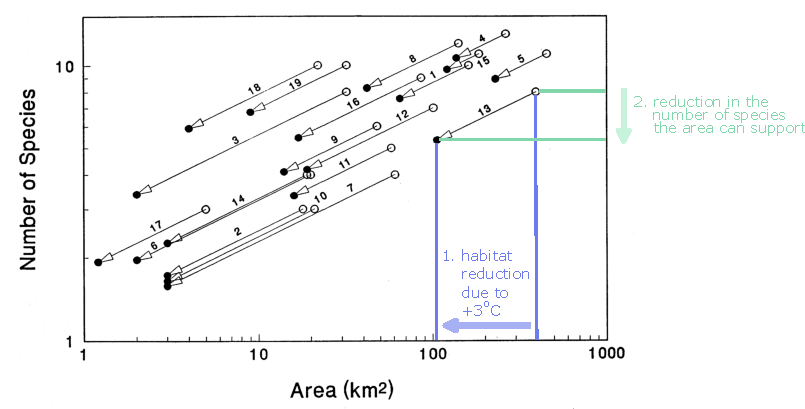
\includegraphics[width=\columnwidth]{figures/methods/fig_ex_macro.pdf}
 \caption[The macroecological approach]{The species-area curve for the distribution of mammal species among isolated mountain ranges. The researchers first used available information to obtain how much habitat loss would cause an assumed $3^{\circ}$C warming.
The arrows represent the changes in both area and number of species resulting from climatic change: the  open circles indicate the current number of species, and the solid circles indicate the predicted number that will persist following a temperature increase. Numbers identify the mountain ranges. Figure adapted from \cite{brown1995macroecology}.}
\label{chp:methods:fig:exmacro}
\end{figure}

Overall, macroecological approaches have led to a paradigm shift because they seek to understand ecological systems through global statistics instead of particular models for each community. Carrying a comprehensive analysis allow researchers to reveal features previously unknown. And this can pave the way for the creation of models and policies.

%%%%%%%%%%%%%%%%%%%%%%%%%%%%%%%%%%%%%%%%%%%%%%%%%%%%%%%%%%%%%%%%%%%%%%%%%%%%%%%%%%%%%%%%%%%%%%%%%%%%%%%%%%%%%
\section{Computational social science}\label{chp:methods:CSS}

\epigraph{A field is emerging that leverages the capacity to collect and analyze data at a scale that may reveal patterns of individual and group behaviors.}{\textit{Lazer et al.} \cite{lazer2009computational}}
Technology has profoundly changed our lives. It is crucial to understand the structure and nature of these changes to face new social challenges such as the  unethical use of communication systems, together with social, economic, and political division. Specially disrupting have been the changes in our communication channels, which can give rise to the spread of fake news, exposition of sensitive and private data, and other cyber risks.\\

The introduction of information and computation technologies (ICT) has also come with new tools to tackle the challenges it has generated.  ICT generate data, \textit{big} data, which can provide insight into the processes at the societal level. We can take advantage of this massive amount of data to create predictive and explanatory models of society. This new approach to the study of society has been called Computational Social Science \cite{lazer2009computational,lazer2020computational}. \\

Computational social science is an interdisciplinary discipline that combines social science research with complexity  and computer science to provide new insights into human behavior and society. The fact that computational social science involves several other disciplines is rooted in the nature of social systems themselves. Essentially, social systems are inherently complex, since they present emergent phenomena, and interdependencies
and feedback across the micro and macro levels of organization \cite{conte2012manifesto}.\\

\begin{figure}[t]
     \centering
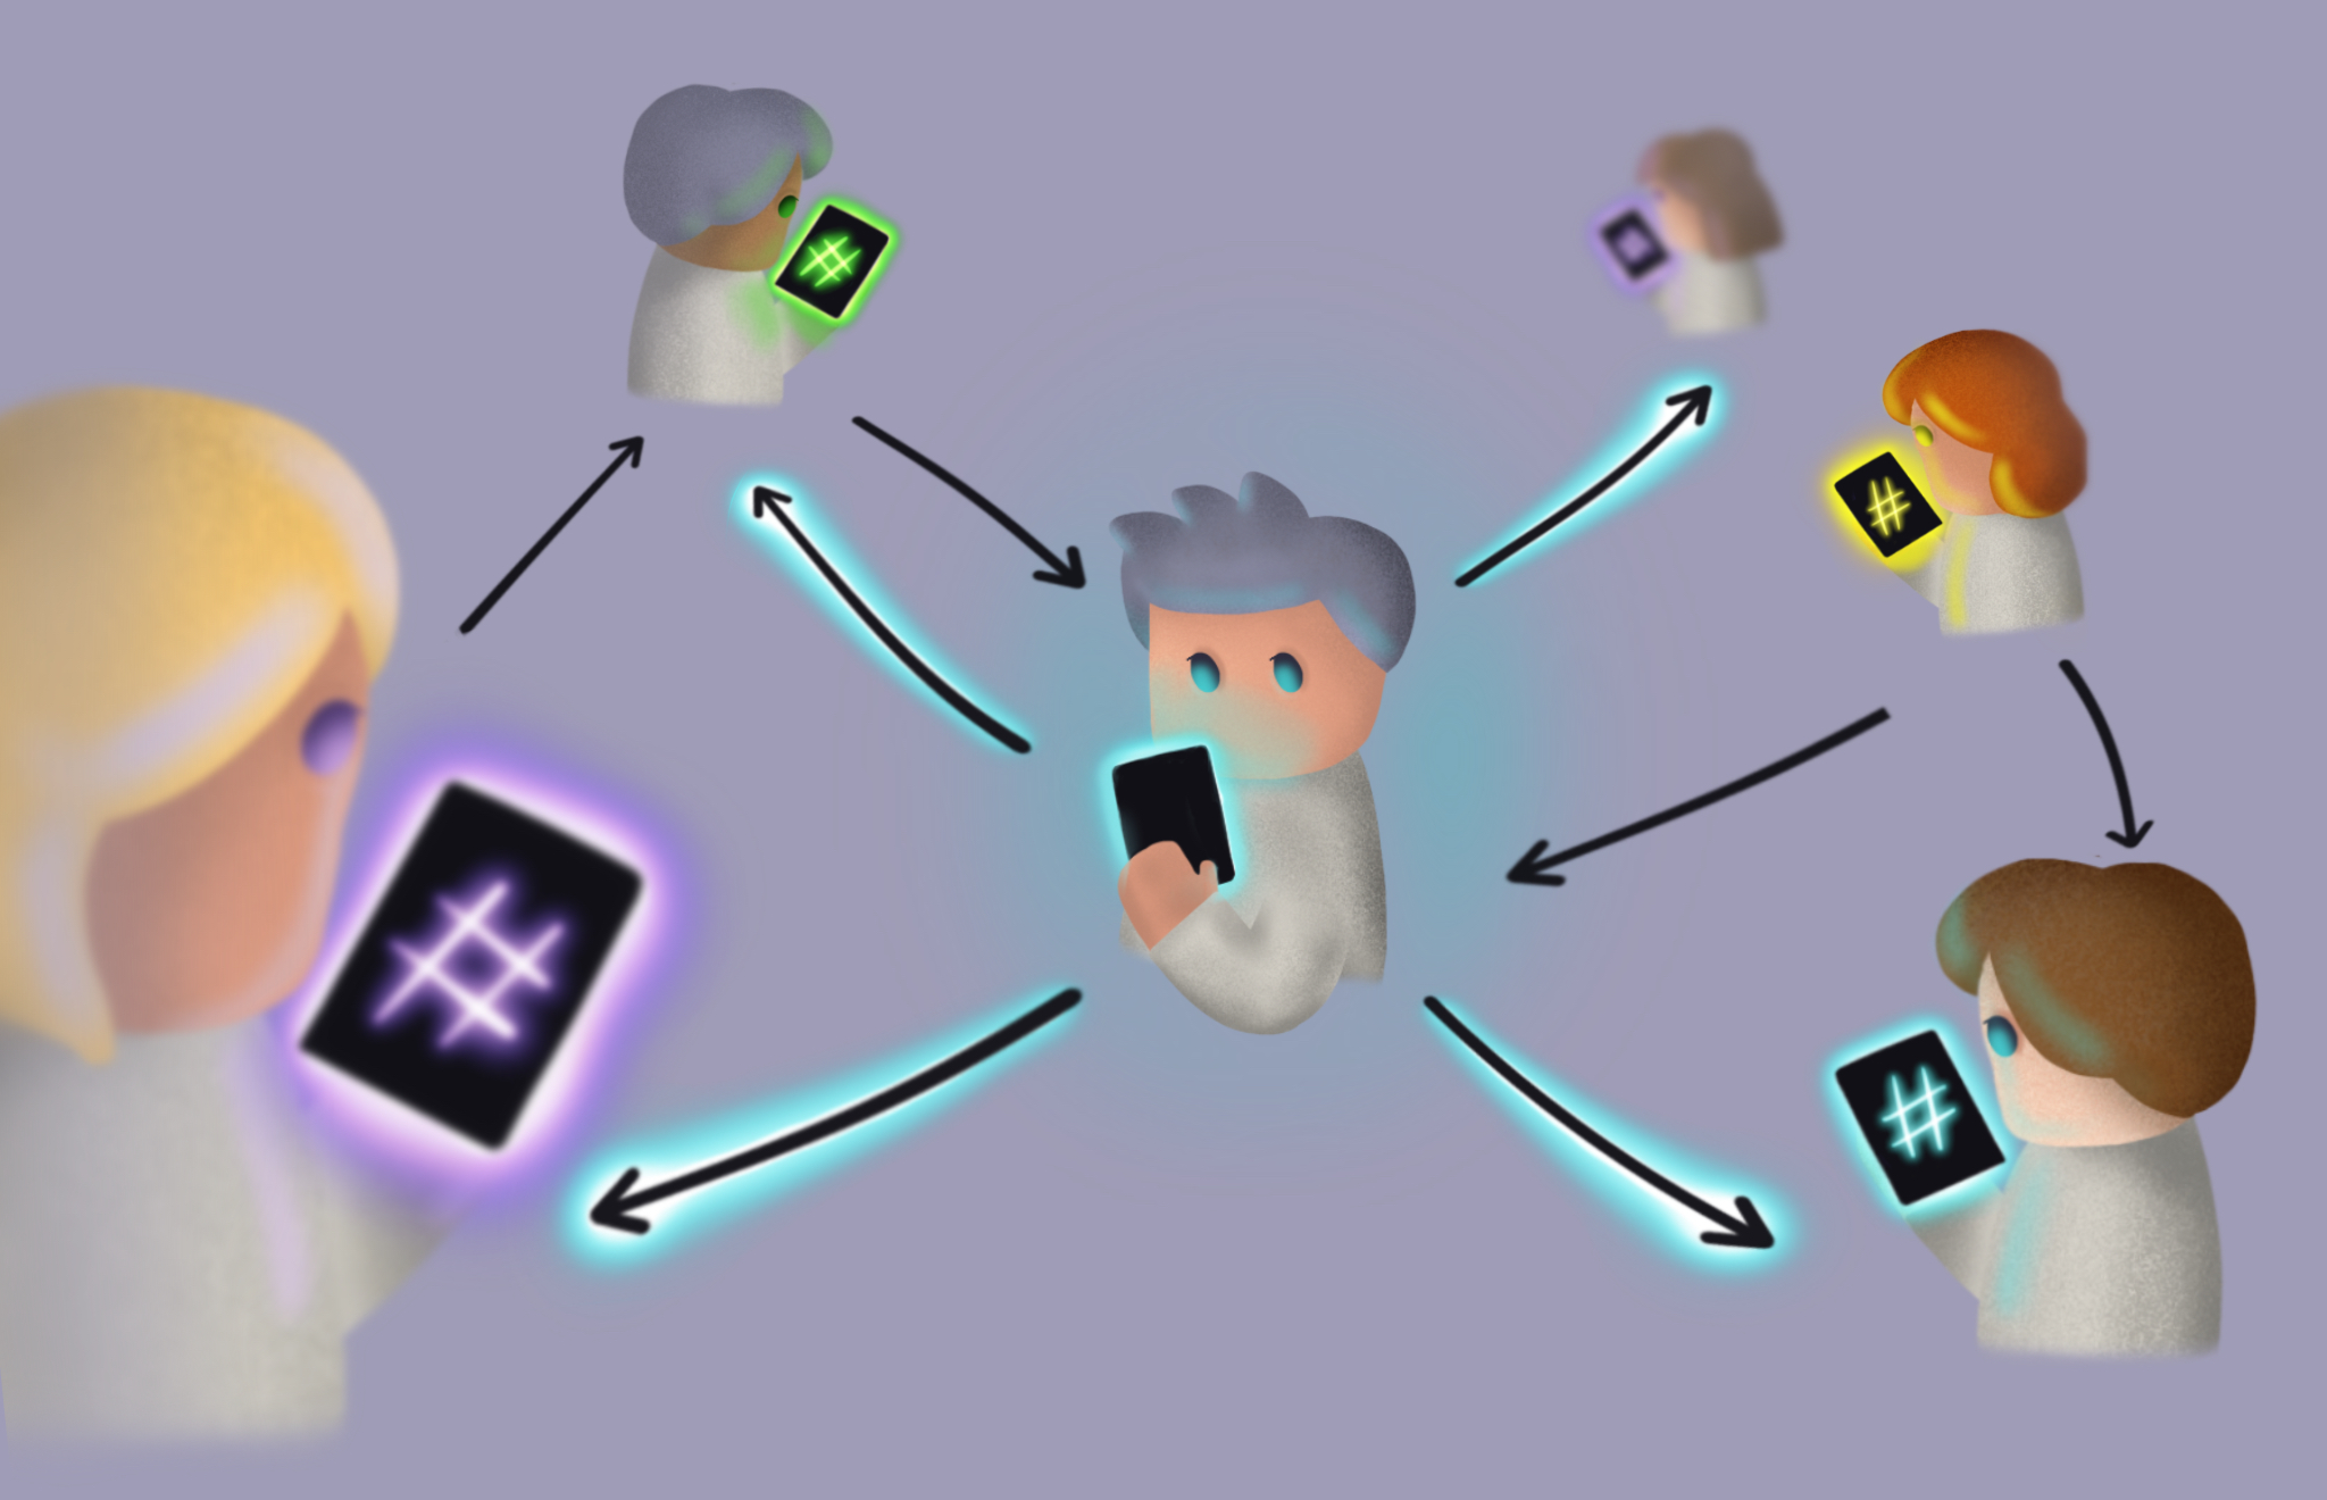
\includegraphics[width=0.8\columnwidth]{figures/methods/fig_neutral.pdf}
 \caption[Online social network dynamics]{Online social networks have been recently studied in computational social science. They are virtual structures made of individuals using the Internet as a communication medium for interacting and sharing content and opinions. Online social networks allow millions 
users worldwide to produce and consume content, providing
access to a vast source of information on an unprecedented
scale. It has become increasingly evident that
competition significantly shapes the structure and the dynamics of these information-driven platforms: users thrive
for visibility, while memes can be thought of as entities that
compete for users’ attention. Each user in the network pays
attention to a finite number of memes constrained by her finite capacity.}
\label{chp:methods:fig:neutral}
\end{figure}

Computational social science uses data from ICT to create quantitative, qualitative, and virtual models, which revolve around some aspects of social systems. For instance, nowadays communication is fast to produce and cheap to consume. This new situation has accelerated the diffusion and contagion of cultural traits in social media. To explain the empirical data that supports the acceleration, mathematical models based on competition for finite collective attention have been proposed \cite{palazzi2021ecological,lorenz2019accelerating}. These models allow us to understand the ups and downs of popular
content and the changes in the online network structure (Figure~\ref{chp:methods:fig:neutral}). \\

The characterization of the propagation of information in social media is another challenge that computational social science is addressing.  It has been discovered that this propagation generates identical macroscopic patterns across different platforms. In turn, the existence of the patterns has helped to discover, using statistical tools borrowed from physics, that bursts of activity in online communication systems can be described by complex contagion dynamics \cite{notarmuzi2022universality}.\\

In this thesis, we address two current challenges of computational social science. We go one step further in the understanding of finite collective attention and propose a model to quantify the competition for this attention in Chapter~\ref{chp:3}. Moreover, to characterize social media, we systematically explore the emergence of universal macroscopic patterns, but using an ecology-inspired framework in Chapter~\ref{chp:4}.

\subsection{Our data}
Beyond the examination of the challenges that computational social science is facing, we now take a closer look at the data that allows us to produce both explanatory and predictive models.  
%In fact,  computational social science aims to take advantage of the data and tools provided by ICT to create  models of large-scale multi-agent systems \cite{conte2012manifesto}. \\

The datasets of both Chapters~\ref{chp:3} and~\ref{chp:4} are from the microblogging platform Twitter. Regardless of its possible bias, Twitter is a liable medium that mimics events occurring in the real world, essentially without delay. This makes the platform an interesting stream of data, offering a machine-readable reflection of current affairs. \\

 Being our objective, broadly speaking, the characterization of online social media, we have analyzed datasets that revolve around events to guarantee that there is a situation where collective attention should be captivated. The datasets greatly differ in their collecting methods, sizes (from $0.2$ to $12$ million tweets), geographical locations (more than $10$ regions involved), time span (from one to $69$ days), and the nature of events, to make the dataset collection as universal and representative as possible.  The datasets consist of a large number of posts (tweets), each with one or more hashtags. In total, $12$ datasets have been used, summing up to more than $55$ million tweets and $4.1$ GB. Specifically, the events collected are: the protests about the self-determination referendum coordinated by the government of Catalonia, Spain, in 2014 \cite{palazzi2021ecological};  the April 2019 Spanish general elections \cite{palazzi2021ecological}; the coverage of Nepal 2015 earthquake; the reactions to the destruction caused by Hurricane Sandy in 2012; the celebration of St. Patrick's Day in 2014; the course of the 2012 UEFA European Football Championship, commonly referred to as Euro 2012; the development of the protests which began in Ferguson, USA, on August 2014 as part of the Black Lives Matter movement; the reaction to the publication of leaked documents known as Panama Papers on 2012; the 2016 United Kingdom European Union membership referendum, often known as Brexit; the 2012 Mexican general elections; and finally, the 2014 Scottish independence referendum
\cite{zubiaga2018}. Another dataset serves as a null model of the other dataset since it is a random sampling from the $1\%$ of all tweets geolocalized in the UK. See Tables~\ref{chp3:tab:datasets} and~\ref{chp:4:tab} for a characterization of the datasets in terms of size.\\
 

 All datasets have been collected through the Twitter Streaming API and are publicly available. The methods of collection consist in filtering certain keywords, official hashtags, or users related to the events. To reduce the artificial presence of the aforementioned sampling hashtags, we have discarded them from our analysis. Hashtags that are not written in Latin script, like Devanagari script or Korean alphabet, have also been cut out because of incompatibilities with character encoding. \\

Finally, tweet ID and  users' data have been anonymized before storage to safeguard privacy; in any case, for each tweet, just the hashtags in the text and the timestamp have been used in our analyses. 


%%%%%%%%%%%%%%%%%%%%%%%%%%%%%%%%%%%%%%%%%%%%%%%%%%%%%%%%%%%%%%%%%%%%%%%%%%%%%%%%%%%%%%%%%%%%%%%%%%%%%%%%%%%%%
\section{Scalings laws in human behaviour}\label{chp:methods:scaling}
It is important to understand the complex dynamics that happen in information ecosystems. Nowadays, our vision of the world is partially obtained through the lens of these digital environments. Political, economic, and other affairs that shape our daily lives also unfold there. The news we read, the songs we listen and the images we share are all memes that have made their path to us.\\

Humans are generating data through communication networks as never before. This causes a bottleneck in our ability to tackle pieces of information \cite{lorenz2019accelerating}, the so-called memes. Online communication systems have reacted to this by becoming an environment where memes compete for users' attention. Regardless of the particular details of the social interaction, the survival of a meme can be thought of as depending on attracting attention.\\

However, extracting useful information from the digital stream has proven difficult. There are too many details to account for and they are intricately entangled. One celebrated solution to these problems is the use of neural networks and machine learning. These algorithms create inference models, classifiers and interpolate data with great ease. Nonetheless, they are black boxes that tell us little about the governing processes. If we want to characterize the mechanisms that shape our social ecosystems, a more promising approach is to study the patterns that arise in them.\\

Patterns have the unsurpassed ability to set isolated pieces of information in a broader context. They are common regularities whose presence reveals hidden processes. If a pattern is detected in different settings, chances are those systems share common underneath mechanisms. \\

\begin{figure}[t]
     \centering
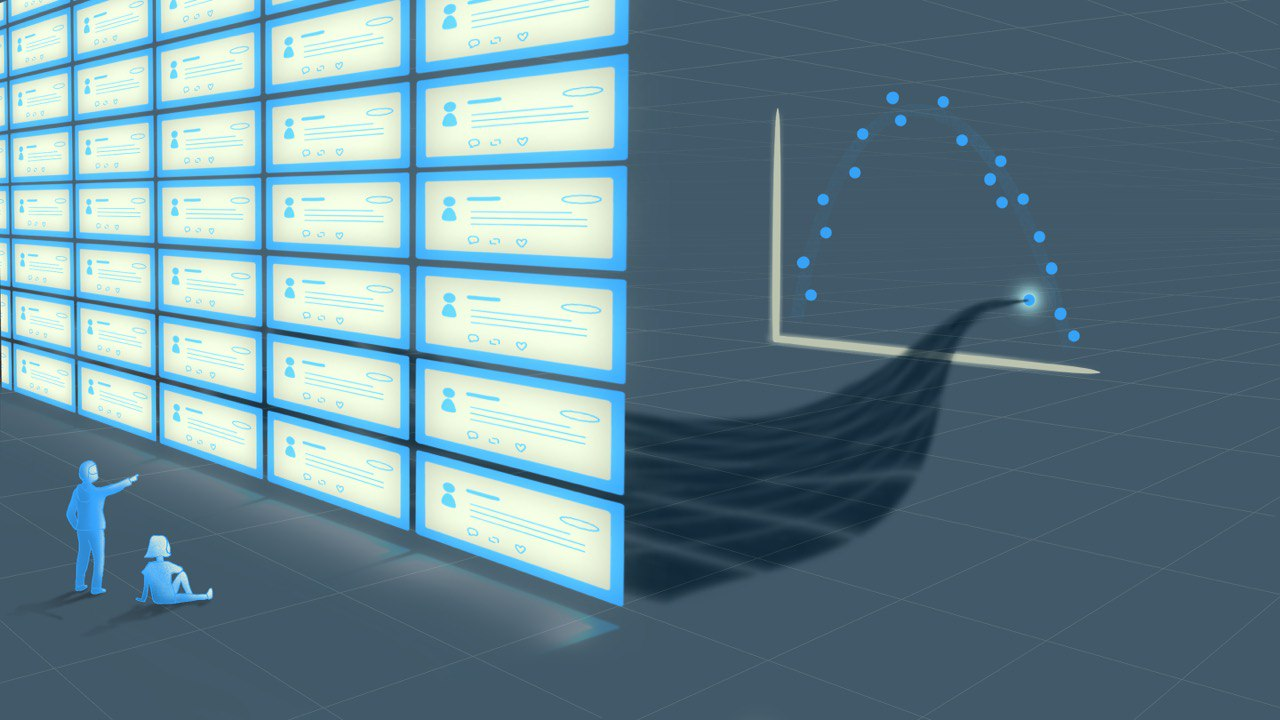
\includegraphics[width=\columnwidth]{figures/methods/fig_TEAMS.png}
 \caption[Patterns from data]{Patterns from data.}
\label{chp:methods:fig:mTEAMS}
\end{figure}

Some statistical relationships already exist in social networks, like Zipf's, Heap's, and Taylor's laws, but it is in ecology where patterns have been exploited for a long time. We have seen in Section~\ref{chp:methods:macro} that there is a complete field devoted to the study of ecological systems by patterns of diversity, abundance, and distribution of species: macroecology.\\

Social systems can also benefit from this statistical framework, despite being firstly designed for ecology. We can map the quantitative characterization of information systems into the study of variation in ecological communities as we presented in Section~\ref{chp:intro:bridge}. We set memes as species. Every time a meme is shared its number of virtual individuals is increased by one and, lastly, the attention problem transforms into species competition for resources.\\

In recent years, some works have applied this approach to disentangle a particular macroscopical property of a social system \cite{plata2021neutral,tovo2021upscaling}. They have studied meme popularity distributions and their persistence on Twitter and predicted the total number of agents from a subsample of emails or Wikipedia articles. However, they have focused only on one or two emergent patterns. To gain a fulfilling insight into information ecosystems, we need to find a complete set of patterns that characterize our systems from all perspectives. Thankfully, an ecological approach is again a promising solution. Ecology is rich in global statistics that can be translated into social systems with our proposed bridge. In this thesis, we plan to test if the patterns found in ecology also hold for human behavior.

%This can allow us to explore how competition for attention in online social networks and the strategies adopted by the users to maximize their visibility shape the structure of our communication dynamics. And going beyond that, how that structure and the amount of competition for attention experienced by users change when exogenous events draw collective attention. \\ ESTO AQUI NO VA
%%%%%%%%%%%%%%%%%%%%%%%%%%%%%%%%%%%%%%%%%%%%%%%%%%%%%%%%%%%%%%%%%%%%%%%%%%%%%%%%%%%%%%%%%%%%%%%%%%%%%%%%%%%%%


\part{Ecological promenade}
\chapter{Structured interactions as a stabilizing mechanism for competitive communities}\label{chp:1}

% One of the critical unanswered challenges in natural sciences is how ecosystems can produce and sustain the astounding biodiversity we observe in nature. This question has drawn interest from a variety of disciplines, including theoretical ecology, mathematics, and physics.  In this context, modeling the stable coexistence of species competing for limited resources is a particularly challenging task. The presence of dominant intransitive cycles in competitive dynamics is one of the processes that make coexistence mathematically possible. However, intransitive interactions frequently end in neutral cycling of species' relative abundance rather than convergence to a stable equilibrium. Though several processes have been proposed in recent years, there are currently few theories that can adequately explain how different species may coexist in competitive ecosystems. Here, we point out that one of the simplest factors promoting stable species coexistence is the locality in their interactions. We investigate a simplified ecosystem in which members of each species are distributed in a spatial network, where interactions are only feasible between nodes that are physically close to one another. The model allows for extrapolation between local and global competition by varying this distance. Our findings show that species may survive and reach a stable equilibrium if two requirements are satisfied. Namely, individuals need to be embedded in space, and they can only interact with other nearby agents. If one of these components is absent, significant oscillations appear.\\

 %In this chapter, the next section introduces our model, followed by the presentation of the results obtained from numerical simulations in Section~\ref{chp1:2}. Our conclusions are then summarized in Section~\ref{chp1:3}.

Ecosystem stability is a persistent question in ecology \cite{May1972,Chesson2018,Allesina2015}. Given the complexity of ecosystems, it is remarkable the biodiversity that they support over extended periods of time. This has led to extensive interdisciplinary research, with many fields of study, such as statistical physics, computer science, and the physics of disordered systems, applying their tools to ecological problems \cite{Bunin2017Ecological,Sidhom2020Ecological,azaele2016neutral}. Over the years, various mechanisms have been proposed to explain the persistence of biodiversity, including random interaction models \cite{May1972} and niche theory \cite{Chesson2018,Bartomeus2018a}. In particular for competitive communities,  higher-order interactions \cite{Grilli2017Higher-orderModels,Losapio2019,Levine2017BeyondCommunities,battiston2021physics} and intransitivity \cite{may1975nonlinear,Laird2009, kerr2002local,maynard2017diversity,buss1979competitive} have been identified as important factors that contribute to maintaining biodiversity.\\

Mathematical models of competitive communities typically assume that one species will dominate and drive all others to extinction, a phenomenon known as the competitive exclusion principle \cite{hardin1960competitive}. However, we do not find this result in natural systems, and hence numerous mechanisms have been proposed to explain the observed diversity of species.  One such mechanism involves the establishment of dominance relationships among species based on a ``Rock-Paper-Scissors'' tournament, in which species $i$ dominates over $j$, $j$ beats $k$, and $k$ is superior to $i$, forming so-called intransitive cycles. Intransitivity, as we mentioned in Section~\ref{chp:methods:intra}, may play a crucial role in promoting species coexistence \cite{may1975nonlinear,maynard2017diversity}, while relative abundances may be shaped by the structure of dominance relationships among species\cite{Laird2009}. Additionally, intransitive tournaments can be defined probabilistically to increase generality. In that situation, one species does not always out-competes others but it does so with a certain probability, allowing for endogenous stochasticity in the dynamics of these systems.\\

Concerning stability, large oscillations in populations are generally viewed as detrimental to biodiversity because they increase the risk of species extinction due to external perturbations. Mathematical models incorporating intransitive dominance often result in species abundances neutrally cycling around an equilibrium point, which is unlikely to occur in natural systems. To address this issue, researchers have proposed various approaches, including the incorporation of higher-order interactions, which involve the modulation of species interactions by other species \cite{Losapio2019,Levine2017BeyondCommunities}. These interactions can lead to convergence towards equilibrium and help to stabilize the dynamics of the system \cite{Grilli2017Higher-orderModels}. This and other approaches focus mainly on interactions between species and ignore that, within species, individual organisms can compete with multiple partners whose identity can change in space (\textit{i.e.} they ignore structured interactions).\\

However, spatial heterogeneity is another factor that can strongly influence species coexistence \cite{valladares2015species,Dieckmann2000,Lowery2019,Travis2005}. The spatial arrangement of individuals can especially impact the magnitude of their mutual interactions, leading to distinct dynamics. For instance, studies have shown that global oscillations in the rock-scissors-paper game can transition to local oscillations when connections between individuals are rewired while maintaining the same number of interactions for each individual \cite{szolnoki2004phase}. In the same way, the nature of ecological interactions can also influence the spatial distribution of individuals. While various studies have identified space as a driver of species coexistence, it is typically considered to only affect biotic or environmental rates in ecological models \cite{Travis2005,Dieckmann2000}. The spatial patterns that emerge are determined by multiple factors, such as self-organization processes \cite{Pascual2002ClusterEcologies}, spatial disturbances \cite{Lowery2019}, early warning signals of ecological transitions \cite{Kefi2007SpatialEcosystems}, and space-dependent ecological interactions \cite{Dieckmann2000}. These factors contribute to the complex interplay between spatial and ecological dynamics, which can have significant implications for the stability and persistence of ecological systems. \\

 Among the spatially dependent ecological process that can have significant consequences for ecosystem coexistence and diversity, we find seed dispersal \cite{Liao2016,Chave2013}, as well as the growth of sessile organisms like corals \cite{buss1979competitive}. From an empirical perspective, experimental studies with three strains of E. coli have shown that the locality of processes can promote diversity through non-hierarchical competition \cite{kerr2002local}. Similarly, in fungi, competition for space with high levels of intransitivity can foster coexistence among different species \cite{maynard2017diversity}. In coral reefs, intransitive patterns of competition for space can decide the final dominant species \cite{buss1979competitive}. These works suggest that space and intransitivity are crucial ingredients for promoting biodiversity. However, even if their effects have been in the spotlight for years \cite{soliveres2018everything}, the question of the role of space in the emergence and maintenance of stability in competitive intransitive communities, as a way to produce structured interactions, has not been fully explored. \\

In this Chapter, we show that space has a stabilizing effect on competitive communities, similar to the effect caused by higher-order interactions, by examining the competitive dynamics that appear from the spatial proximity between sessile individuals. To begin with, we investigate simplified competitive dynamics where pairs of individuals compete for resources through probabilistic intransitive cycles. We introduce space into this framework explicitly by creating an interaction network between individuals, where nodes represent  individuals of different species and links are drawn according to their distance. The spatial arrangement of individuals limits competition to only adjacent neighbors, reducing their mixing. By varying the minimum distance at which links are created, we can interpolate between local and global interactions to study their impact on the dynamics. For instance, when each individual can interact with every other individual in the system, we recover the classical mean-field case for global competition. This context provides a convenient environment to explore whether the spatial distribution of individuals, in combination with the range of competitive interactions, can function as mechanisms for the maintenance of biodiversity, serving as an alternative to higher-order interactions.\\

\section{\label{chp1:1}Building blocks of a stable competitive community}

We analyze an isolated community made up of a fixed large number of individuals $N$ from various $g$ species, and we consider the impact of space in two different factors: the geographical location of the individuals of the different species and the distance up to which they can interact. The first aspect is represented by a network, where each individual occupies a node representing a physical position. Only one individual can be hosted by a node at a time. These spots may be distributed randomly or regularly spaced. Secondly, regarding interactions,  they compete if there is a link between two individuals. Connections are established according to an interaction range, where long-distance contacts increase global competition and lose spatial correlations. Instead, short ranges result in local interactions between nearby nodes, creating what we call ``structured interactions''. \\

  Under these assumptions, our model is appropriate for organisms that are firmly rooted in one location, so possible target
communities are those mainly governed by local interactions such as shrubs, grasslands, and plants with clonal growth \cite{Dieckmann2000}.
  
\begin{figure}[htbp]
 \centering
 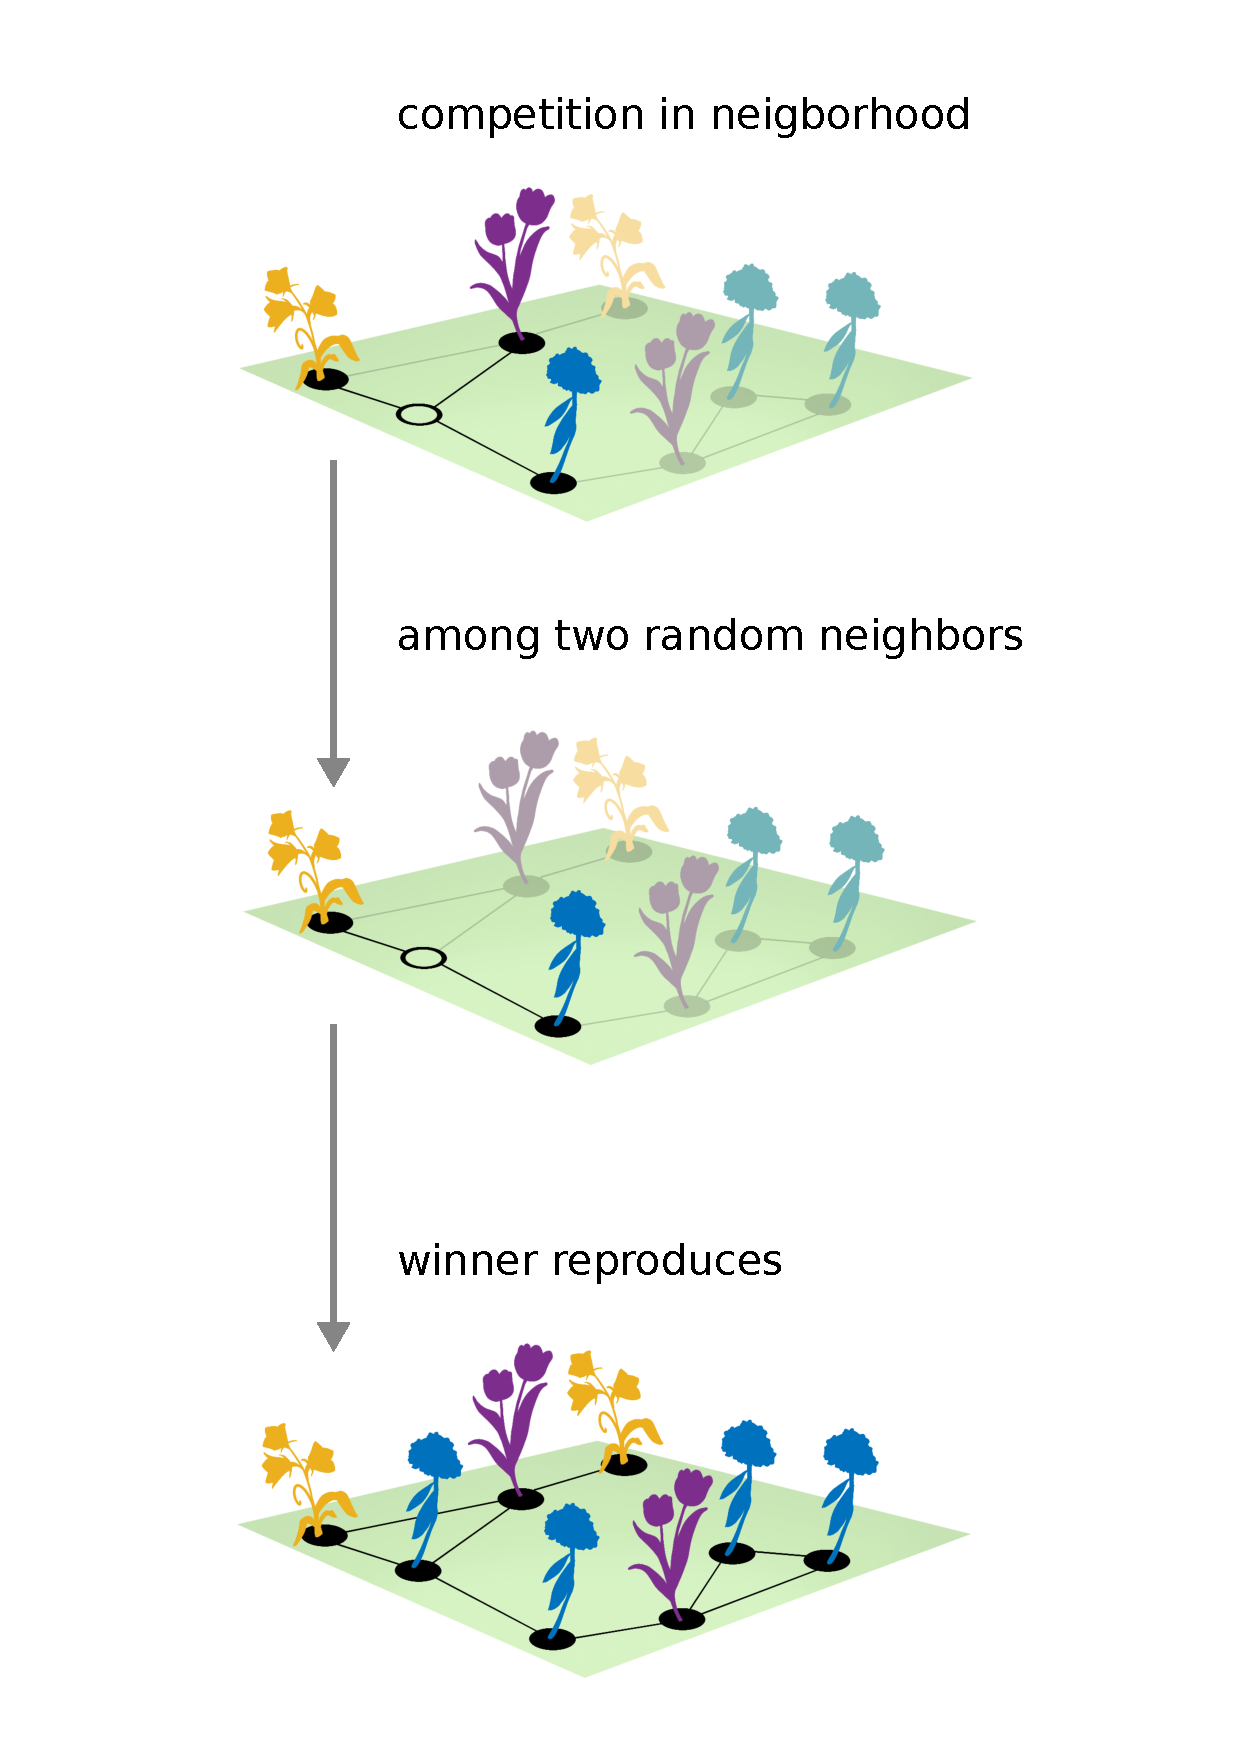
\includegraphics[width =0.8\textwidth]{figures/chp1/fig1.pdf}
 \caption[Competitive dynamics model]{Competitive dynamics are represented schematically in the diagram. We describe the model through the example of plants competing in a forest. With probability $1/N$, a random plant dies, leaving an empty fertile place (an empty node). Of the three neighbors, two of them are chosen at random (highlighted in the center Panel) to compete for placing their seedlings there. The winner is then selected based on the probabilities of the species dominance matrix $H$, and its descendant grows in the empty node. }
 \label{chp1:fig:1}
\end{figure}


\subsection{\label{chp1:1.1}Competitive Dynamics}
 To focus on the relationship between stability and space, we consider a minimal model for competitive communities. Specifically, there are only two ecological processes at play: death (with mortality rates equal for all species) and competition. At each time step, an individual dies, leaving a vacant location that becomes immediately available. This ignites competition among its neighbors to reproduce and fill the location. The neighbors are the individuals within an interaction range that can reach that location. Two of them are randomly selected and compete for placing a descendant. The winner is chosen using a dominance-matrix approach, explained below, and its offspring matures in the next time step (Figure~\ref{chp1:fig:1}). \\

 The $g \times g$ dominance matrix $H$ encodes the winning probability of an individual of species $i$  in competition against an individual of species $j$. The values of $H_{ij}$ for $i> j$ are extracted at random from a uniform distribution [0,1]. We then set  $H_{ji}=1-H_{ij}$, and $H_{ii}  = 0.5$. With these conditions, coexistence is reached when $H$ presents intransitive dominance cycles \cite{Grilli2017Higher-orderModels,Allesina2015PredictingWebs}. Intransitive cycles of competitive dominance occur when $H_{ij} > H_{jk}> H_{ki} > 0.5 $ for some triad $i,j,k$. See Section~\ref{chp:methods:intra} for a short introduction to the importance of intransitivity in ecological systems. \\

To assure the replicability of our results in the numerical simulations, we set $g = 3$ and the following matrix $H$ for our numerical simulations:
 \begin{equation}
 H = 
 \begin{pmatrix}
0.5 & 0.34 & 0.76 \\
0.66 & 0.5 & 0.25 \\
0.24 & 0.75 & 0.5 
\end{pmatrix}. \label{eq:H}
 \end{equation}
Moreover, our conclusions remain valid independently of the number of species and the precise form of matrix $H$ as long as it contains intransitive cycles.

%Moreover, the ecosystem is constrained to have an odd $g$ in the long term in agreement with the equivalent replicator dynamics in \cite{Grilli2017Higher-orderModels}:
%\begin{equation}
%    \frac{d x_i}{ dt} = x_i \sum_{ij} W_{ij} x_j,
%    \label{eq:Pgrilli}
%\end{equation}
%where $W = H-H^t$. The result derives from the fact that Eq.~\ref{eq:Pgrilli} only has an equilibrium $x^*_i \geq 0$ if the dimension of $W$ is odd when $W$ is antisymmetric.  When one species goes extinct, another extinction event must occur to keep the number of species odd.
%



%(from draft_v2)Competitive relationships are hence neither completely  hierarchical nor intransitive and encoding the competitive relationships as the probabilities $H_{ij}$ allows us to range from neutral to complete dominance. The elements $H_{ij}$ are not $\pm 1$ or $0$ as in others intransitivity models \cite{Laird2009}, but take account of a probabilistic intransitivity

\subsection{Interactions' structure}
Once defined the competitive dynamics we model the effect of space. In particular, space is involved in two ways to explore its effect on the dynamics. It is present through the nodes' physical layout and by the distance upon which individuals can compete.
To explore the effect of different spatial arrangements, we employ three different types of networks: a 2D square lattice, an Erd{\H{o}}s-R{\'e}nyi graph, and a Random Geometric Graph (see Section~\ref{chp:methods:networks} for a more detailed description of the networks). \\

%TEXTO INICIAL ANTES DE PASAR PARTE A LOS METODOS: 
%The \textit{2D square lattice} serves as the standard for the most ordered space because of its simplicity and widespread application in ecology \cite{Dieckmann2000,grimm2005IBM,Lowery2019}. Its nodes are discretely and consistently spaced from one another on the unit square. The eight adjacent nodes are thought to be a node's closest neighbors (considering periodic boundary conditions) (left graph of Figure~\ref{chp1:fig:2}a). The 2D lattice, whose nodes are regularly distributed and connected, generates strong spatial correlations.
The \textit{2D square lattice} is our null model of a highly ordered space due to its simplicity and widespread application in ecology \cite{Dieckmann2000,grimm2005IBM,Lowery2019}. It generates strong spatial correlations because nodes are regularly distributed and connected on the unit square (Figure~\ref{chp1:fig:2}a). 

On the other extreme, \textit{Erd{\H{o}}s-R{\'e}nyi graphs} (ER)\cite{erdos1959random} are our baseline for non-spatial interactions. Nodes are randomly connected with probability $p$, regardless of their location (Figure~\ref{chp1:fig:2}c). Consequently, there are no spatial correlations.

Finally, the \textit{Random Geometric Graph} (RGG) \cite{Dall2002RandomGraphs} is a compromise solution in respect of structure and randomness. Nodes are randomly distributed in the unit square and connect if their Euclidean distance is smaller or equal to an interaction radius $R_{RGG}$ (Figure~\ref{chp1:fig:2}b). This point makes an RGG very versatile. Although the network has a disordered structure, it shows strong spatial correlations because of the interaction radius, which allows us to tune continuous distances and investigate the variability in the number of neighbors \cite{cardillo2012,estrada2016,arias2018}.  We have set in this graph, and in the lattice, periodic boundary conditions to avoid irregular properties in the limits of the square. A node very close to the bottom will connect with a node high at the top. \\

Summing up, the ER graph serves as our null model as it lacks spatial structure. The \textit{2D square lattice} represents highly regular interactions, while the RGG strikes a balance between the two models. \\

\begin{figure}[htbp]
 \centering
 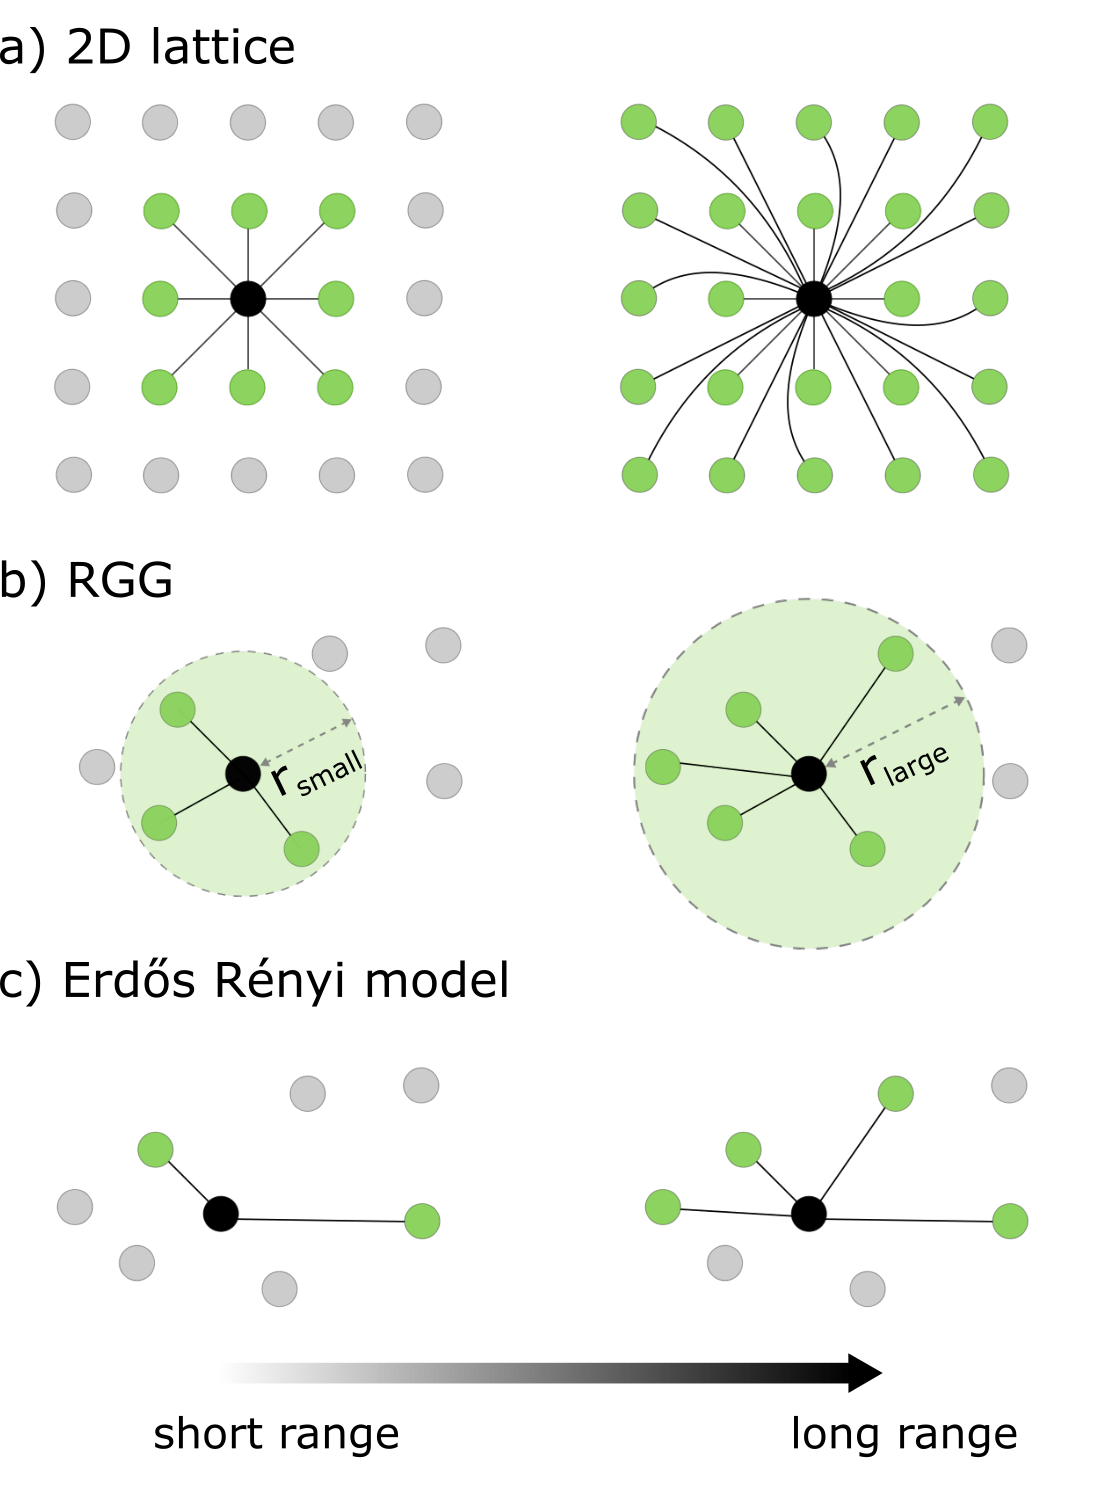
\includegraphics[width =0.75\textwidth]{figures/chp1/fig1.png}
 \caption[Spatial interaction networks]{The three spatial interaction networks under consideration. The black node's neighbors are shown in green for various interaction ranges. (Panel a) The 2D lattice has a homogeneous distribution of nodes. The neighborhood on the left side of the Panel corresponds to the shortest interaction range, and on the right side, we see how it increases when the smallest interaction range has been raised by one unit. (Panel b) For the Random Geometric Graph (RGG), the coordinates of the nodes are set uniformly
 at random in the unit square. Two nodes are linked together if their
 distance is less than $R_{RGG} = r_{small}$ (left side of the Panel)
 or $R_{RGG} = r_{large}$ (right side). (Panel c) The Erd{\H{o}}s-R{\'e}nyi
 graphs do not have any spatial structure because, with probability
 $p$, a pair of nodes is connected regardless of their distance. In Panel c, nodes present the spatial arrangement as in Panel b, but now the neighborhood
 of the black node is randomly determined by linking probabilities
 $p = 0.2$ and $p = 0.4$, respectively.
}
 \label{chp1:fig:2}
\end{figure}
Once defined the structures of our interactions, we now turn to the question of how space is involved in the creation of the links. The interaction range tackles precisely this problem. The range determines who interacts with whom and, ultimately, it defines the individuals that compete for a vacant location that another leaves when it dies. When the interaction range is short, only close nodes compete. More distant nodes join the competition as the range grows, and eventually, the neighborhood size will be large enough to cancel out the influence of nodes' location. Finally, for every network, we trivially get all-to-all competition with the largest interaction range. At that point, we can consider the system to be well-mixed. \\

We regulate the competition from local to global in the different networks by modifying the interaction range. In particular, for square lattices, increasing the interaction range $R_{2D}$ sets connections not only between the nearest nodes but also the second, the third groups of closest neighbors. In the same way, long-range interactions in an RGG are obtained by increasing the interaction radius $R_{RGG}$. In ER networks, node distances do not play any role. Increasing the connection probability $p$ creates larger neighborhoods, but the locations of the neighbors are random. Thus, to compare results across the different network models, it is convenient to quantify the interaction range by the mean degree $\langle k \rangle$. Table~\ref{chp1:tab:1} summarizes the main features of the networks and provides the relationship between the interaction range and $\langle k \rangle$, while the right column of Figure~\ref{chp1:fig:2}a-c gives a glimpse of how the networks look after increasing the interaction range.

\begin{table}[t]
\centering
\caption[Spatial features of network models]{Spatial features (or their absence) of the three considered network models. Further details are explained in Section~\ref{chp:methods}. The average neighborhood size is denoted by $\approx \langle k \rangle$.}
\label{chp1:tab:1}
\begin{tabularx}{\textwidth}{X X c X c}
\hline
\textbf{Network}    &\textbf{Parameter}  &  \textbf{Space}  & \textbf{Connections} & \textbf{$ \langle k \rangle$} \\ \hline \hline
2D lattice & interaction radius, $R_{2D}$  &   ordered     & Chebyshev distance  & $\sum_{r = 1}^{R_{2D}} 8 r$              \\ \hline
RGG        &  interaction radius, $R_{RGG}$  & random    & Euclidean distance  & $\pi R_{RGG}^2(N-1)$                \\ \hline
ER         &    connection probability, $p$   & random & random              & $\approx p(N-1)$  \\
\hline
\end{tabularx}
\end{table}

\section{\label{chp1:2}Results}
%%%%%%%%%%%%%%%%%%%%%%%%%%%% RESULTS
Once the model has been defined, we begin an extensive analysis of it using Monte Carlo simulations. At the start of each simulation, species inside each node are initially assigned at random with  uniform probability $1/g$. The variable $n_{i,\nu}$ will take the value of 1 if species $i$ is present at node $\nu$, and $0$ otherwise. Since a node can only host one individual at a time, then $\sum_i^g n_{i,\nu}=1$, $\forall \nu$. We use an asynchronous update (each time step, just one node is selected to die) and define a generation as $N$ updates. To ensure that on average every node has experienced death events, we simulate during at least $N$ generations. Lastly, we monitor the relative abundance of individuals of each species in the system $x_i(t) \equiv N^{-1}\sum_\nu^N n_{i,\nu}$. \\

To help understand the  macroscopic state of the system, we employ the relative abundances $x_i$. In fact, since for every $t$, we have $\sum_{i}^{g} x_i(t) = 1$, this expression means that the relative abundances represent a point in the $(g-1)$-simplex (the portion of the $\sum_{i=1}^{g} x_i=1$ plane which $x_i \geq 0, \, \forall i$). The vertices of the simplex, in particular, correspond to a population of just one species. As time evolves, the variation in relative abundances follows a trajectory confined in the simplex. These trajectories characterize the state of the system and therefore the simplex may be seen as a representation of the phase space. \\

\begin{figure*}[t!]
     \centering
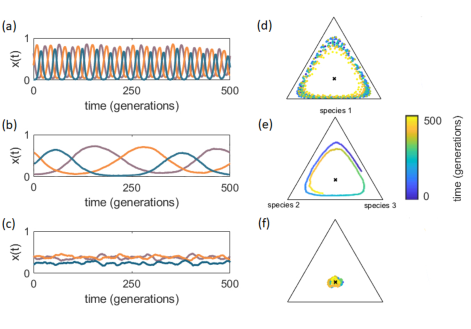
\includegraphics[width=1.1\textwidth]{figures/chp1/fig3.pdf}
 \caption[Temporal evolution of relative abundances and simplex representation]{(Panels a,b,c) Temporal evolution of relative abundances $x(t)$ for the different interaction scenarios in a RGG with $ N = 10^4$. (Panel a) All-to-all interactions: individuals compete for any empty node as the radius covers the whole plane ($R_{RRG} = R_{max} = \sqrt{2}$). (Panel b) Long-range interactions: the radius is reduced to $R_{RGG} = 0.15$, which corresponds to an average degree $\langle k \rangle \simeq 706$. These two radii create a similar scheme in that the community lacks structure and leads to wide oscillations. (Panel c) Short-range interactions: now $R_{RGG} = 0.03$ and $\langle k \rangle \simeq 28$. In this situation, the system is spatially structured and abundances do not heavily fluctuate. (Panels d,e,f) The trajectories of the left Panels are represented on the 2-simplex (the region of the $x_1 + x_2+ x_3 = 1$ plane in which $x_1,x_2,x_3 \geq 0$). The view of the plots is set perpendicular to the simplex plane. Abundances oscillate in wide cycles around what seems an equilibrium point (black cross) for all-to-all (Panel d) and long-range interactions (Panel e). When interactions are short-range (Panel f), abundances are restricted to an area close to the equilibrium. For all Panels, the trajectories are displayed once the transient has vanished.}
\label{chp1:fig:3}
\end{figure*}
\subsection{\label{chp1:2.1}Temporal evolution}

To begin our analysis, we look at the temporal evolution of species abundances for the most straightforward scenario of three competing species, $g=3$. Unless otherwise noted, we always employ the same dominance matrix, given in Eq.~\eqref{eq:H}, which produces results that are typical of any other randomly generated $H$ with competitive intransitive cycles. We find that the behavior through time varies depending on the spatial distribution of species (the networks) and the proximity of their interactions (the interaction range). \\

Cycles of wide amplitude in species abundances occur in communities with no spatial structure, as ER graphs or for all-to-all interactions (Figure~\ref{chp1:fig:3}a). Large fluctuations can also be seen in structured communities (RGG and 2D lattice) with long-range interactions. This behavior is consistent with the mean-field approximation's prediction of the dynamics (see Appendix~\ref{appen:MF}). However, the amplitude of the oscillations is unaffected by the initial conditions, suggesting that they are limit-cycle oscillations, which are qualitatively distinct from the neutral oscillations anticipated by the mean-field theory. \\

Differently, in the two spatial networks considered, decreasing the interaction range reduces the amplitude of the oscillations. For a sufficiently short range,  abundances only slightly fluctuate in the vicinity of an equilibrium state, as it can be seen in Figure~\ref{chp1:fig:3}c.  \\

The value of that state is, for all analyzed cases, the equilibrium fixed point obtained from the mean-field approximation (which is $(x_1,x_2,x_3)=(0.374, 0.383, 0.243)$ for the matrix $H$ in Eq.~(\ref{eq:H})). Returning to the oscillatory case, we also recover the same values if we calculate the temporal average of the relative abundances for the same matrix $H$.  \\

These findings call for further analysis since they show a non-trivial dependence of the dynamics with the interaction range. In the next Subsections, we systematically examine the impact of the interaction range and network structure on the dynamics of the species.

\subsection{\label{chp1:2.2}Dynamical behavior depends on structured interactions} 

As a first step towards getting a better understanding of the dynamics, we define a measure to characterize the system's behavior for each interaction range and structure. In this case, the magnitude of the oscillations is not a reliable indicator because of the stochastic simulations' noisy dynamics. Thus, we focus on the mean area encompassed by the system's trajectory on the simplex, which is measured according to Appendix~\ref{appen:AreaSimplex}. The intuition for this choice is that a trajectory takes up a limited area when the system fluctuates with small amplitude around some equilibrium abundances,  (Figure~\ref{chp1:fig:3}f), whereas larger oscillations cover much broader areas (Figure~\ref{chp1:fig:3}d,e).  \\

After we've established our metric for describing the dynamics, we can study the impact of space. To do so, we keep $H$ fixed across all simulations while changing the interaction range for each type of graph. This procedure allows us to alter the underlying network structures, and go from highly-structured communities to systems for which the effect of space is diluted due to the large interaction range. The ER graphs, however, pose a problem since we are unable to define distances across them. For those graphs, we utilize the degree as a substitute for the interaction range. This substitution is feasible because the interaction range determines both the distance up to nodes compete and their degree. In that way, we can now compare the results for the ER graphs with the two spatial networks.  \\

\begin{figure}[t!]
    \centering
    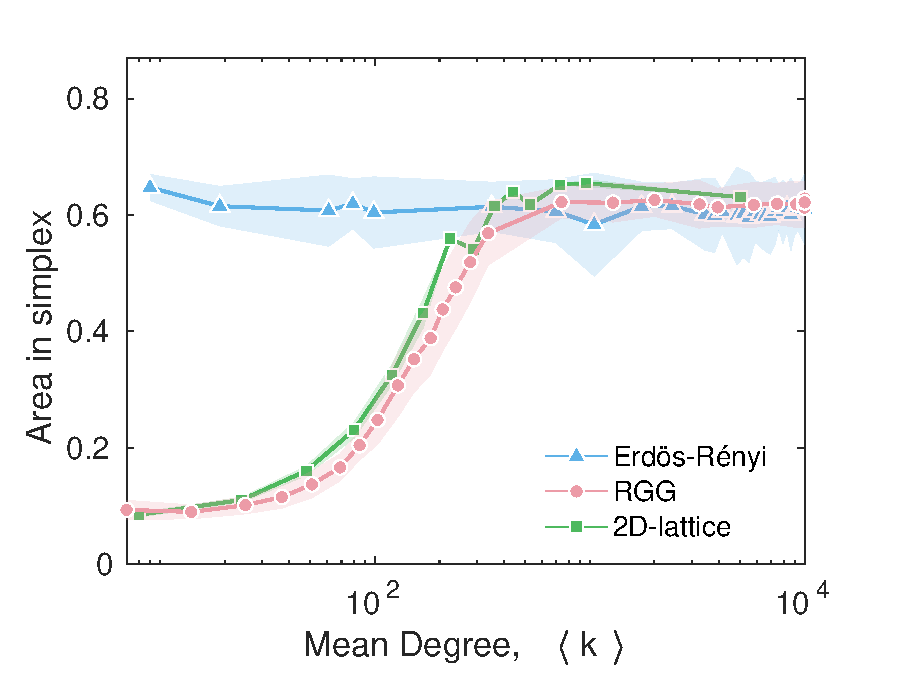
\includegraphics[width=0.8\textwidth]{figures/chp1/fig4.pdf}
    \caption[Impact of average degree on the area in simplex]{Average area inside the trajectory over the 2-simplex of a 3-species community as a  function of average degree $\langle k \rangle$ for the different networks of $N = 10^4$ nodes. The dominance matrix $H$ of Eq.~(\ref{eq:H}) is used for all networks. Each point represents the mean area over $50$ simulations, each starting with different initial conditions and network structures. The areas have been calculated excluding the $5\%$ of out-layer points of the trajectories. Shades indicate the $95\%$ confidence interval. The procedure to compute the areas from time series is explained in Appendix~\ref{appen:AreaSimplex}.}
    \label{chp1:fig:4}
\end{figure}

We start by simulating the ER graphs, i.e. the situation where the system has no spatial structure (blue marks in Figure~\ref{chp1:fig:4}). We increase the average degree to focus solely on the effect of the interaction network, leaving aside any spatial constraints. The simulations present large oscillations for all values of the degree. These wide fluctuations translate into high area coverage for all interaction ranges and, therefore, we can conclude that the size of the neighborhood does not affect the dynamics. \\

However, this picture changes totally when we consider spatially structured interactions. In both the RGG and 2D lattice, the systems show different behavior for short interaction ranges, that correspond to having a low mean degree. In that regime, the dynamics stabilizes around the equilibrium (the cross in Figure~\ref{chp1:fig:3}), covering a tiny area in the phase space (pink and green points in Figure~\ref{chp1:fig:4}). However, as we increase the interaction range and hence increase $\langle k \rangle$, the results of the ER networks are recovered, and we observe large oscillations again. For both networks, the transition between these two regimes occurs when the average degree is $ 50 \lesssim \langle k \rangle \lesssim 100$ for a network of $N = 10^4$ nodes.
 
As a result of these findings, the following intuitive picture emerges: when we consider long-range interactions --e.g. large mean degrees--  we obtain large oscillations, regardless of whether the networks have spatial structure or not. The period and  amplitude of these oscillations are independent of the initial conditions, which suggests they are of the limit-cycle type. In the limit of long-range interactions, the mean-field approximation is expected to be valid, and indeed it correctly predicts the oscillatory behavior (see Appendix~\ref{appen:MF}). But this approximation fails to give the limit-cycle behavior as it predicts instead neutral oscillations. On the other hand, when we constrain competition to short-range interactions, the dynamics stabilize around some fixed point $x^*$ if and only if the networks have some spatial structure by construction, i.e. for the RGG and 2D lattice. \\

Lastly, to test the robustness of our results we also investigated the influence of the model's parameters. Varying the number of individuals $N$ does not strongly modifies the shape of the curve, just it becomes more gradual for larger $N$. The results are still qualitatively the same. We also found results that were nearly identical when $g = 5$ (not shown), except for a higher probability of extinction due to long-range interactions.

\subsection{\label{chp1:2.3}Spatial configurations}

So far, only the behavior  of the species relative abundances $x_i$ has been explored, showing a dependency on the spatial fabric of the networks the species are competing in. To understand this behavior, we turn to directly observe the spatial organization of the species. In Figure~\ref{chp1:fig:5}, we show two different snapshots of a 3-species community in a 2D square lattice. The two images only differ in the interaction range. \\

%To better understand the mechanism behind the reported behavior, we show in Figure~\ref{chp1:fig:5}.

With short ranges (Figure~\ref{chp1:fig:5}a), species form mono-specific patches. Inside the patches, death events  do not contribute to variations in relative abundance because competition is among individuals of the same species. And hence, changes in $x_i$ can only happen along the patches' borders, where different species are in contact. This characteristic makes patches more robust to invasion from other species. In turn, it decelerates the dynamics and reduces the possibility of large oscillations.  \\

\begin{figure*}[t!]
 \centering
  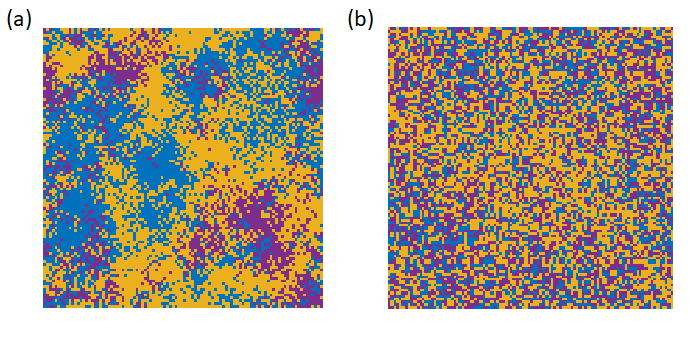
\includegraphics[width=1.0\linewidth]{figures/chp1/fig5.png}
\caption[Spatial organization for different interaction radius]{Spatial organization of a 3-species community in a 2D lattice of $N=10^4$ and dominance matrix $H$ of Eq.~(\ref{eq:H}). Each species is depicted with a different color, matching Figure~\ref{chp1:fig:3}a-c. (Panel a) Short-range interactions: only the $8$ closest neighbors at distance $R_{2D} = 1$ compete for the vacant node left by an individual when dies (see the left graph at Figure~\ref{chp1:fig:2}a). (Panel b) Long-range interactions: $360$ neighbors ($R_{2D} = 9$) participate now in the competition. Videos for the two ranges of interactions are publicly available in \cite{videos}.} \label{chp1:fig:5}
\end{figure*}

With long-range interactions (Figure~\ref{chp1:fig:5}b), vacant nodes can be reached by many individuals from different species, blocking the formation of single-species clusters. The lack of patches would avoid reaching a steady state, generating large-scale oscillations: the homogeneous solution predicted by mean-field theory. Videos of the temporal evolution in the two regimes are available \cite{videos}. \\

The latter results of Figure~\ref{chp1:fig:5} imply that short-range interactions decrease the system's effective competition by lowering the probability of interactions between individuals of different species. To confirm this hypothesis, we compute $\langle P_{ij} \rangle$, the average probability that species $i$ and $j$ compete for a vacant node when interactions are short. This probability is calculated numerically by keeping track of how many times species $i$ and $j$ have been chosen to compete, and then averaging across the simulation's duration. We then compare it with the expected value for the all-to-all case $\overline{P}_{ij}$ that simply is the product of the relative abundances of species $i$ and $j$ at the mean-field equilibrium, i.e. $\overline{P}_{ij}=x_i^* x_j^*$.  \\

In our example system from Eq.~(\ref{eq:H}), we have

$x^*=(0.374, 0.383, 0.243)$, thus:
 \begin{equation}
\overline{P}_{ij} =
\begin{pmatrix}
0.1399 & 0.1432 & 0.0909\\
0.1432 & 0.1467 & 0.0931\\
0.0909 & 0.0931 & 0.0590
\end{pmatrix} 
\label{eq:mata2a}
\end{equation}
And the obtained matrix $\langle P_{ij} \rangle$ in a RGG with short-range interactions ($N = 10^4$, $R_{RGG} = 0.022$ and $\langle k \rangle \simeq 15$) is:
\begin{equation}
\langle P_{ij} \rangle =
\begin{pmatrix}
\textbf{ 0.2160} & 0.0965 & 0.0597\\
 0.0965 & \textbf{0.2241} & 0.0659\\
 0.0597 & 0.0659  & \textbf{ 0.1156}
\end{pmatrix} \ ,
\label{eq:matshort}
\end{equation}
where same-species competition $\langle P_{ii} \rangle$ has been highlighted in boldface. \\

We observe that intra-species competition $\langle P_{ii} \rangle$  has a significantly higher probability to occur than the inter-species competition (the off-diagonal terms $\langle P_{ij} \rangle$) for short-range interactions than in the all-to-all case. This shows that the patches, created exclusively in structured communities with short-range interactions, reduce the effective inter-specific competition.  \\

\begin{figure}[t!]
 \centering
 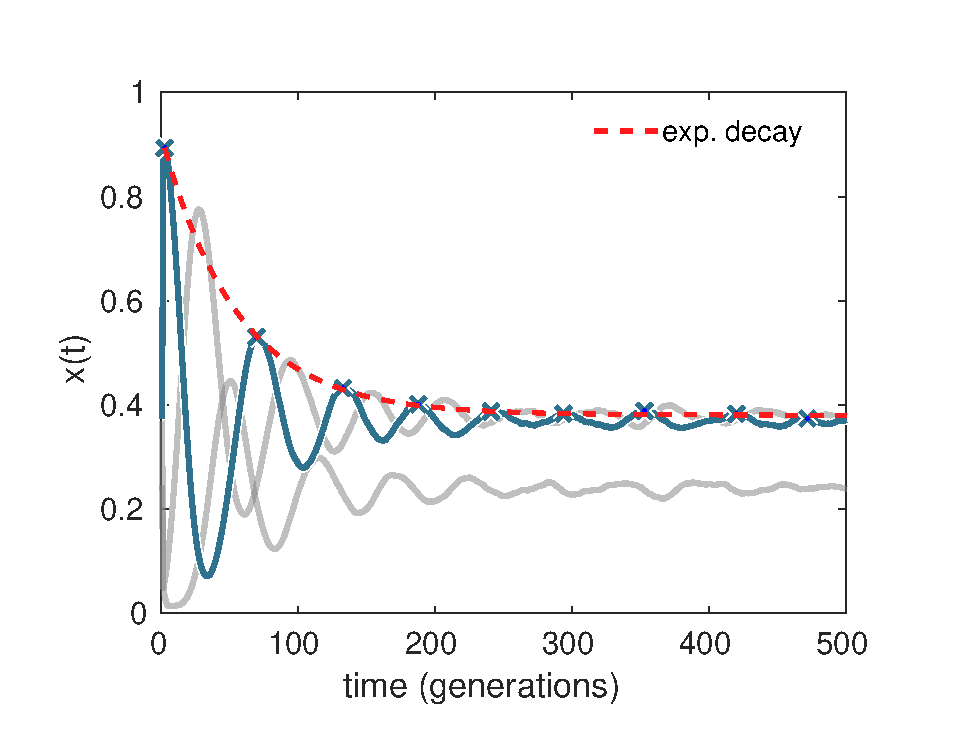
\includegraphics[width=0.8\textwidth]{figures/chp1/fig6.pdf}
  \caption[Time evolution of the recovery from a pulse perturbation]{Recovery from a $90 \%$ pulse perturbation in a 3-species system with $H$ from Eq.~(\ref{eq:H}). The relative abundance of the blue species is artificially boosted from its equilibrium value to be the $90 \%$ of the entire population, while the  other species' relative abundances (in gray) are proportionally reduced. The system is embedded in an RGG of $10^4$ nodes and $R_{RGG} = 0.03$. The red curve is the fit of the local maxima of the relative abundance (blue crosses) to the exponential function, resulting in $a e^{-\alpha} + b$ with $\alpha = 0.018$, $a = 0.53$ and $b = 0.38$.}
    \label{chp1:fig:6}
\end{figure}

\subsection{\label{chp1:2.4}Stability and fluctuations}

Once understood the mechanism responsible for the stabilization of the dynamics in the short-range regime, we turn to check
the stability of that regime. To do so, we investigate how the system reacts to pulse perturbations of various intensities. In the simulations, this is done by imposing an abrupt change in one species' abundance and recording the time required to return to the original state. More precisely, the abundance of a random species is suddenly increased to cover a large portion of the system, while the other species' abundances are proportionately decreased. In Figure~\ref{chp1:fig:6}, we show the evolution 
after a $90 \%$ perturbation of one species'  abundance in an RGG with $R_{RGG}=0.03$ (short range). The system returns to equilibrium while the disturbance decays exponentially. So Figure~\ref{chp1:fig:6} demonstrates that the dynamics can bounce back even with such a large perturbation. \\

\begin{figure}[t!]
 \centering
 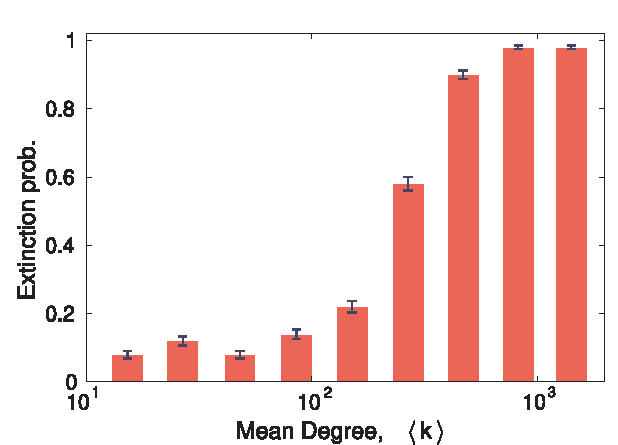
\includegraphics[width=0.8\textwidth]{figures/chp1/fig7.pdf}
  \caption[Extinction probability as a function of the average degree]{ Extinction probability as a function of the average degree. We have varied the interaction radius from short to long ranges. The communities are in an RGG of $N=10^4$ individuals governed by $H$ from Eq.~\eqref{eq:H}. Each red bar corresponds to the mean over $50$ different networks --different simulations-- and the error bars are the $95\%$ confidence intervals.}
    \label{chp1:fig:7}
\end{figure}

However, perturbations could also lead to extinctions since we are simulating a finite system. In such a scenario, the latter fixed point for the macroscopic variables $x_i$ would be lost. To examine when this case occurs, we systematically measure the probability of extinction of one species after a pulse perturbation as a function of the mean degree. In particular, we define the probability of extinction of one species as the fraction of simulations in which at least one species gets extinct following a perturbation. Starting with a $N=10^4$ community in an RGG, we measure those probabilities for increasing interaction radius after a $90\%$ perturbation. Consistently with the previous results, Figure~\ref{chp1:fig:7} shows that the probability falls to less than $10\%$ for small degrees, but extinctions are almost certain for larger neighborhoods, making the long-range interaction regime not robust. \\

\begin{figure}[t!]
 \centering
 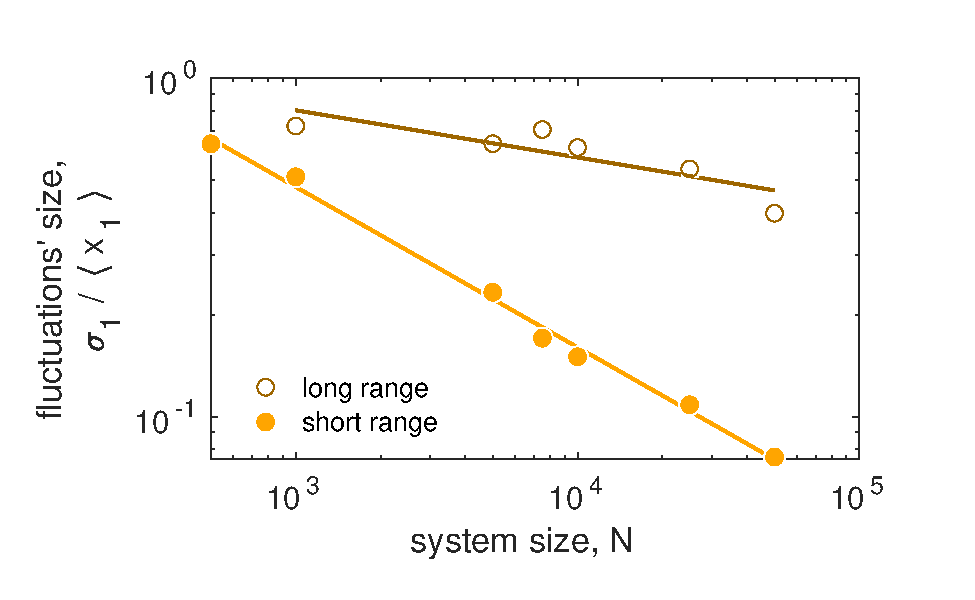
\includegraphics[width=0.8\textwidth]{figures/chp1/fig8.pdf}
  \caption[Interplay between fluctuations' scaling and system size]{Fluctuations' scaling as a function of the system size $N$. We choose the coefficient of variation of species 1 ($\sigma_1/\mean{x_1}$) to be a proxy for fluctuations. Each point is the average over $10$  simulations where the variance $\sigma_1$ and mean relative abundance $\mean{x_1}$ have been calculated over at least $\Delta t = 10^8$ time-steps after the transient. Communities with short-range interactions have an average degree $\langle k \rangle = 15 \pm 2$, and decrease their fluctuations with the size of the system as $\sigma_1/\mean{x_1}\sim N^{-0.47}$, consistent with a scenario with no correlations. For the settings with long-range interactions ($\langle k \rangle = 980 \pm 190$), the scaling of the relative fluctuations goes as $N^{-0.14}$. The simulations have been performed over RGG, with $g =3$ and $H$ of Eq.~(\ref{eq:H}), as usual.}
    \label{chp1:fig:8}
\end{figure}

Finally, we conclude our analysis by studying the nature of the fluctuations around the equilibrium for both short and long-range interactions. To do so, we measure how the size of the fluctuations scales with the system's size. The size is defined as the coefficient of variation of the relative abundance of each species $i$: $\sigma_i/\langle x_i \rangle$. Figure~\ref{chp1:fig:8} shows the scaling for one species in RGG of different sizes and interaction ranges. For short-range interactions, which produce small degrees ($\langle k \rangle = 15 \pm 2$), we observe a scaling exponent of $0.47$. The value is pretty close to $0.5$, the one expected for residual fluctuations that arise from the stochastic noise due to the finite size of the system. As a result, the possibility that the observed fluctuations were truly oscillatory behavior of small amplitude is ruled out. In turn, for networks with larger degrees ($\langle k \rangle = 980 \pm 190$), we find an exponent of $0.14$. In this situation, fluctuations represent an actual ecological signal that results from the interactions in an environment with high mixing. \\

\section{Discussion}
 \label{chp1:3}

Many attempts have been made to provide a biological basis for the robustness of biodiversity in natural ecosystems, especially for those communities governed by competition. Here, we have demonstrated that spatial interactions alone lead to the stability of multispecies communities by a minimum model of intransitive competition. \\
 
We have analyzed  a model where individuals compete in a structured environment with intransitive dominance cycles. We have compared different spatial configurations, from regular lattices to random connections that outweigh the effect of space. Our results reveal that spatial interactions confined to nearest neighbors promote the stable coexistence of different species, while long-range interactions cause species' relative abundances to fluctuate endlessly. \\

 By focusing on the spatial organization of the individuals, we found that local interactions enable species to survive by forming mono-specific patches, that decrease the effective competition experienced by each individual because it only happens at their borders. This clustered configuration slows down the dynamics, dramatically damping out fluctuations and leading to stability. Per contra, mean-field approximations of the dynamics do not match the latter results. This is, however, not unexpected given how much the dynamics depend on the spatial correlations that the short-range interactions produce. \\





\chapter{Structural predictors of species survival in complex ecological communities} \label{chp:2}
We have commented that explaining the emergence of biodiversity in ecological communities has been a long-standing challenge. In Chapter~\ref{chp:1}  we tackled this issue by introducing a model of intransitive competition, which highlighted how local spatial interactions can lead to stable coexistence. However, despite that  coexistence has been long sought after in ecological systems, environmental perturbations and temporal changes can cause species to go extinct. Observations about the drivers behind species' extinction have significant consequences for biodiversity dynamics and conservation issues. With this in mind, our focus in this Chapter will be on identifying what structural factors better explain extinctions. To do so, we increase our scale of description and model communities at the level of species, which is the unit in which we assess biodiversity.\\

 Over the years, the structure of the network of species interactions has proven to play a crucial role in the stability and resilience of ecosystems, so it is a natural place to look for a priority list of which species to protect \cite{Holme2021NetworksConsequences}. Since the structure arises from the position of the species in the interaction network, a recurrent approach is to rank the species according to some topological measure \cite{McDonald-Madden2016UsingEcosystems,Keyes2021AnLosses}. Some works investigate also other characteristics besides topological features, such as ecological functions \cite{Jordan2008IdentifyingNetworks} or connectance after deletion \cite{Torres-Alruiz2013AIndexes}. A follow-up approach has been to combine these indices \cite{ Gouveia2021,Estrada2007CharacterizationSpecies} and estimate their relative importance, measuring correlations or using machine learning \cite{Gouveia2021}.\\

However, in these topological approaches, two important aspects intrinsic to ecosystems are often neglected. First, the dynamics that are embedded in the network of interactions. Species abundances naturally fluctuate through time, especially if exogenous events like perturbations or species removal occur. The above research usually studies the bare network structure, removing species and their links at discrete time steps, without taking abundance evolution into account. Secondly, there is a bias towards focusing mainly  on trophic interactions \cite{Allesina2009GooglingCoextinctions,Estrada2007CharacterizationSpecies,Keyes2021AnLosses,Torres-Alruiz2013AIndexes,Jordan2008IdentifyingNetworks,Gouveia2021} or ``extended'' food webs, which include resources \cite{Bellingeri2013RobustnessResources} or ecosystem services \cite{McDonald-Madden2016UsingEcosystems} --benefits that humans derive from nature such as food.\\

One explanation for these tendencies may be the fact that studying the relationship between the structure and dynamics of networks, on one side, and more types of interactions, on the other, complicate both the empirical and theoretical analysis. Nevertheless, including other kinds of interactions (such as non-trophic ones) has proven to radically change our understanding  of ecosystems \cite{pocock2012robustness, Fontaine2011TheNetworks, Kefi2015NetworkShores, Garcia-Callejas2018ThePersistence,kefi2012more,bartomeus2021experimental}. Furthermore, in the stage of uncertainty that we are entering with climate change, it is more important than ever to understand how to maintain biodiversity. While predictions of the effects of climate change on species typically focus on its direct impact on individual species, the influence of species interactions should not be overlooked. Species interactions can significantly affect the propagation of this impact to other organisms at all levels by altering community structure and dynamics \cite{gilman2010framework}. \\

In this Chapter, we take a step in the direction of integrating these missing ingredients in the context of environmental change. We aim to discover what are the structural properties that have the species that survive in a community with several types of interactions simultaneously. More specifically, we study what are the structural characteristics that better predict the fate of species whose abundances are evolving in a community where both competition and mutualism are present and that have suffered a perturbation. These non-trophic interactions are thought to play a crucial role in biodiversity and shape the interaction network's architecture \cite{Wang2021InterspecificNetworks,Gracia-Lazaro2018TheEcosystems,bastolla2009mutualism,pocock2012robustness}. We not only include several types of interactions, but also a population dynamics over several underlying network structure. Our analysis encompasses  diverse structures, from  random models to empirical networks, and different interaction intensities to simulate changes in the environment. Moreover, the importance of these structural characteristics, which we define as ``structural predictors'' in the sequel, is ultimately quantified by a decision tree, a type of machine learning algorithm. \\

We find that when only one type of interaction is considered, a single predictor can predict species survival. 
%We find that traditional communities with only one kind of interaction, i.e. only mutualism or only competition, have a single predictor. 
This predictor is different for each type of interaction but it is preserved through the studied network topologies. However, there is no universal predictor when multiple types of interactions are present within the same network. In that sense, each community is unique and has a particular set of node characteristics to assess their species' vulnerability. The set is usually composed of measures that combine network structure with the strength and sign of the interactions. This contrast of results emphasizes how crucial it is to consider the various types of interaction and their strength to advance our understanding of ecological communities.


\begin{comment}
NB: We are studying communities, not ecosystems. \\
papers mainly from: https://docs.google.com/spreadsheets/d/1bq7Vr6msYC6TfhEUPycKtHFvbeKh-8Kq1DP-7Io-qZA/edit?usp=sharing

\textbf{AIM:}
We aim to discover what are the structural characteristics that have the species that survive after an environmental change.

\textbf{IMPORTANCE:} 
- for ecosystems' management: ''these would then be a priority list of what nodes to protect '' from \cite{Holme2021NetworksConsequences}

\textbf{NOVELTY}: key \textbf{differences} with our approach:
0) Usually, do not take dynamics into account, only structure.
1)  when there is dynamics, they run the dynamics until it has stabilized and them, perturb the system. our approach is radically different, as we do not care on the previous equilibrium (does it even exist). We start our simulations right after the perturbation.
2)  Moreover, this perturbation is  usually targeted, ie ''let's remove one random species'' or ''from high to low degree'' or ''one by one''... We let the dynamical system to extinct species.
3) we study several interactions ''at the same time'': mutualism and competition, no food webs!

\textbf{definitions to explain}=
	- persistence
    - make clear what we mean by structure (sometimes called topology) ''positional properties of its species''

\textbf{previous works:}
Lots of works only focus on \textbf{structure without dynamics}, also known as topological approach:
	- they study vulnerability to extinction cascades: \cite{Allesina2009GooglingCoextinctions,Sole2001,Keyes2021AnLosses,Bellingeri2013RobustnessResources,Donohue2017LossCascades}). 
	- and species/ecosystem service/management  action  ranking according to some measure: \cite{Estrada2007CharacterizationSpecies,McDonald-Madden2016UsingEcosystems,Jordan2008IdentifyingNetworks,Keyes2021AnLosses}

Some other papers \textbf{combine structural indices} \cite{ Gouveia2021,Estrada2007CharacterizationSpecies} but in order to estimate the importance, they just correlate (except \cite{Gouveia2021} that uses ML but only with structural measures), we a DT, finer.
- some papers look also at other characteristics of the species besides simple topological features:
		- \textbf{function}\cite{Jordan2008IdentifyingNetworks}
        - \textbf{connectance} after deletion \cite{Torres-Alruiz2013AIndexes} (they call them ''dynamics'')

Focus mainly on 
- \textbf{foodwebs} \cite{Allesina2009GooglingCoextinctions,Estrada2007CharacterizationSpecies,Keyes2021AnLosses,Torres-Alruiz2013AIndexes,Jordan2008IdentifyingNetworks,Gouveia2021} 
- and ''extended food webs''(FW+servises \cite{McDonald-Madden2016UsingEcosystems}, FW+resources \cite{Bellingeri2013RobustnessResources}).	

but... Studying  \textbf{several types of interaction}s (in a community) makes more difficult to find universal structural predictors of survival after an environmental change. necessity and dangers of studying multiple interactions at a time!
	- kefi \cite{Kefi2015NetworkShores}
    -callejas 2018 \cite{Garcia-Callejas2018ThePersistence}
    - from hugo: In ecology, however, there have been
few empirical examples that have considered multiple types
of interactions within the same network, probably because
of the high logistic effort involved in documenting all the
potential interactions present within a community (Melián
et al. 2009, Pocock et al. 2012). Furthermore, the analysis
of these networks presents some difficulties over the analysis
(like the use of multilayer networks, Mucha et al. 2010,
Boccaletti et al. 2014, Kivelä et al. 2014).

\textbf{Concepts that are related}: cascades of extinctions, robustness, perturbations, fragility, vulnerability to species losses, keystone species.
\end{comment}


\section{Ecological communities model}

%We study the impact of the structural properties of a species on its survival in a community that  includes several interaction types simultaneously.  
Our communities consist of $n$ species that can interact mutualistically as well as competitively. Not every species interacts with each other, but the interactions create a complex network (described in Section~\ref{chp2:2.1}). Every species is characterized by its frequency $x_i$, which is influenced by its mutualistic and competitive interactions following a replicator dynamics (Section~\ref{chp2:2.2}). The structural properties that will be tested as possible predictors of survival are defined in Section~\ref{chp2:2.3}, and the algorithm to test their predictive importance is presented in Section~\ref{chp2:2.4}.

\subsection{Structure: Artificial and Empirical Ecological Networks  } \label{chp2:2.1}

We use networks to describe the structure of the interactions in ecological communities. Each node represents a species, and links document the presence of an interaction. The links can be positive (mutualistic) or negative (competitive) since our subjects of study are communities governed by non-trophic interactions. The nature of the interactions also makes it appropriate to set undirected links, contrary to trophic networks.\\

 Being our main objective to study real communities, we beguin with the construction of simple artificial networks and then build up adding realism till studying, in the end, empirical networks. The parameters of the network models have been set to match those of the empirical counterparts, and to be large enough to provide enough statistics. 

\subsubsection{Random networks}
We have chosen three random models to mimic different connection patterns. Their topologies represent particular properties of how species can interact. As outlined in Section~\ref{chp:methods:networks} of our methods, we will employ the following network models: Erdös-Rènyi model, which serves as null model of ecological networks; the Barabasi-Albert model, which has a scale-free degree distribution; and the Holme-Kim model, which is more realism because presents clustering among species. While the Barabasi-Albert model creates tree-like structures that may not capture the common motifs in nature,  clustering is especially relevant for competitive communities with intransitive or diffuse competition  \cite{godoy2017intransitivity,losapio2019perspectives}, and networks that integrate different interaction types \cite{kefi2016structured} like plant spatial association networks \cite{Saiz2017EvidenceNetworks}.

%\paragraph{1) Erdös-Rènyi model:}  The first studied network structure is the Erdös-Rènyi graph \cite{erdos1959random}, where nodes are connected at random according to a linkage probability $p$. It is typically used  as a null model because the properties of its nodes behave nicely around well-defined average values.
%\paragraph{2) Barabasi-Albert model:} The second step in complexity is to simulate scale-free networks. The underlying motivation is the fact that the presence of generalists and specialists tend to create heavy-tail degree distributions. In particular, we have implemented the preferential attachment model of Barabasi-Albert \cite{Albert2002StatisticalNetworks}. 
%\paragraph{b) Holme-Kim model:} To add up more realism, we use the Holme-Kim model \cite{Holme2002GrowingClustering} because it grants clustering among the species. The previous scale-free model creates tree-like structures that may not represent the common motifs usually present in nature. Especially, competitive communities with intransitive or diffuse competition  \cite{godoy2017intransitivity,losapio2019perspectives}, and networks that integrate different interaction types \cite{kefi2016structured} like plant spatial association networks \cite{Saiz2017EvidenceNetworks}.
 
\subsubsection{Empirical networks}
Along with the artificial networks, we also test our results against different empirical networks representing competitive and mutualistic assemblages. Specifically, we use two different datasets, each one applying a different technique to build the interaction networks. By doing so,  we prevent our results from being biased towards a particular method for inferring interactions. The criteria for choosing these networks have been that they should be connected and have a large number of species, as both conditions ensure well-defined node properties. A complete list of the networks can be found in  Table \ref{tab:empnetworks}. 

\paragraph{(A) Pollination and seed-dispersal networks:} We have chosen networks based on interaction frequencies from the open database of ``Web of Life'' \cite{weboflife}. 
%The networks have only two types (guilds) of nodes (e.g. plants and pollinators, or plants and seed-dispersers), and mutualistic links are only set between nodes of different guilds. 

The networks consist of two types of nodes, $A$ and $B$, that  interact positively with one another. If $N_A$ and $N_B$ denote the number of species in each set, then $n = N_A + N_B$ is the total number of species. These sets represent guilds, for example, plants and pollinators, or plants and seed-dispersers. Mutualistic interactions are only present between nodes of different guilds, and therefore they are fully encoded in a bipartite matrix. 

To infer competition among species that use a common resource, we have supposed (following the logic of the works  \cite{Gracia-Lazaro2018TheEcosystems} and \cite{Wang2021InterspecificNetworks}) that competition arises within guilds.
Two nodes of the same guild will be linked if they share a minimum number of common connections with nodes in the other guild. The threshold on the minimum number of common mutualistic neighbors is set for each network one by one and depends on $n$ and the network connectance. With this procedure, called one-mode projection \cite{Newman2010}, we represent the hypothesis that two species that share a mutualistic partner compete for the resources it provides. For example, there is apparent competition among plants when they have common pollinators, since they try to exclusively secure the pollinators' service during the blooming season. Conversely, intra-guild competition arises among pollinators to get nectar before it's too late, or among seed-dispersing birds for eating the seeds \cite{Wang2021InterspecificNetworks}. In Figure~\ref{chp2:fig:1}, for instance, the first two blue nodes have a negative link because they share the first yellow node as a mutualistic partner. 

\begin{table}[htbp]
\caption[Properties of the empirical networks]{Properties of the empirical networks used in this work. Networks of type (A) are obtained from ``Web of Life'' \cite{weboflife}, and encompass pollination (pol.) and seed dispersal (s.d.). Networks of type (B) are from \cite{Saiz2017EvidenceNetworks}. $S$ is the number of species (network size); $C$ is the connectance (defined as the proportion of links between species that are realized); $R$ is the ratio of total mutualistic and competitive links.}
\label{tab:empnetworks}
\begin{tabularx}{\textwidth}{ c c c  c c X X X} 
 \hline
  & Type & $S$ &  $C$ & $R$  & Location & Ref. \\ 
 \hline\hline
 $\texttt{Emp}$\_$\texttt{IL}$ & (A) pol. & 1500 &  0.03  & 0.36  & Illinois, USA & \cite{robertson1928flowers} \\ 
 \hline
   $\texttt{Emp}$\_$\texttt{P16}$ & (A) pol. & 205 &  0.035 & 0.63  & Doñana Nat.~Park, Spain & \cite{herrera1988pollination}\\ 
 \hline
 $\texttt{Emp}$\_$\texttt{S22}$ & (A) s.d. & 317 &  0.06  & 0.27  & São~Paulo, Brazil & \cite{silva2002patterns}\\ 
  \hline
  $\texttt{Emp}$\_$\texttt{P48}$ & (A) pol. & 266 &  0.05  & 0.28 & Denmark & \cite{dupont2009ecological} \\ 
  \hline
   $\texttt{Emp}$\_$\texttt{P49}$ & (A) pol. & 262 &  0.362 & 0.45 & Denmark & \cite{bek2006pollination}\\ 
  \hline\hline
   $\texttt{Emp}$\_$\texttt{CG}$ & (B) & 117 & 0.059  &  0.67   & Cabo de~Gata, Fraile, Spain & \cite{Saiz2017EvidenceNetworks}\\ 
 \hline
   $\texttt{Emp}$\_$\texttt{CGR}$ & (B) &  104 &  0.044 & 1.22 & Cabo de~Gata, Romema, Spain & \cite{Saiz2017EvidenceNetworks}\\ 
 \hline
   $\texttt{Emp}$\_$\texttt{MOP}$ & (B) &  42 &  0.11   & 2.69 & Monegros, Planerón, Spain & \cite{Saiz2017EvidenceNetworks}\\ 
 \hline
   $\texttt{Emp}$\_$\texttt{MOS}$ & (B) &  75 &  0.066 & 1.12  & Monegros, Sariñena, Spain & \cite{Saiz2017EvidenceNetworks}\\ 
   \hline
   $\texttt{Emp}$\_$\texttt{AE}$ & (B) &  56 & 0.066 & 0.68  & Estepa, Spain & \cite{Saiz2017EvidenceNetworks}\\ 
   \hline   
\end{tabularx}
\end{table}

\paragraph{(B) Spatial association plant networks:} 
Giving that interaction networks are, after all, based on proxies, we have also used the empirical networks constructed by spatial co-occurrence (see Section~\ref{chp:methods:networks})  from \cite{Saiz2017EvidenceNetworks}. In that work, the authors built several plant communities from arid ecosystems in Spain. Nevertheless, the ecosystems present differences in abiotic and biotic conditions, including steppes and shrublands. 

Note that, unlike in the previous set of networks, there are not any guilds and thus we loose the block structure of the adjacency matrix. An example of such networks is given in Figure~\ref{chp:methods:fig:hugo}. \\

%\paragraph{(C) Spatial association plant networks:} Finally, we use empirical networks from \cite{Garcia-Callejas2021TheConstraints}, which have been constructed by a method that polishes and merges the other two approaches. It combines normalized observed interaction frequencies, phenological overlap and the quantity of shared resources. The proxies, combined together, infer plant-plant and plant-pollinator interactions. 

 %from  Mediterranean grassland communities
 
% NEW: For example, assuming that there are not preempting processes (i.e. the amount of soil water, light or food is not altered by earlier taxa), then species within the same guild will not compete for common resources if they do not overlap phenologically

These methods for reconstructing empirical networks are  not exempt  from  limitations, and we have addressed some that could affect our study in Appendix~\ref{appen:Inferring}. 

\begin{figure}
    \centering
    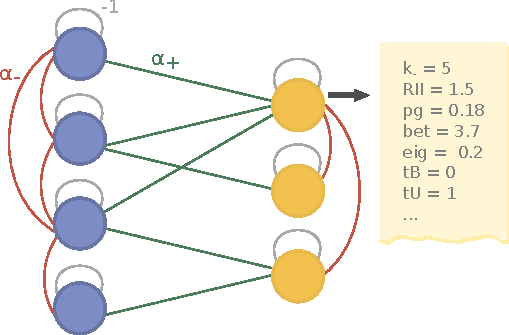
\includegraphics{figures/chp2/fig_1.pdf}
    \caption[Simple network of a community with two guilds]{Simple network of a community with two guilds (blue and yellow nodes). Species are nodes connected to themselves by gray loops, representing the regulatory effect  of  a  species  on  itself. Red links depict competitive interactions of strength $\alpha_-$ and green links refer to mutualistic interactions of strength $\alpha_+$. Competitive links have been drawn whenever two nodes in one guild share a neighbor in the opposite guild. For each node, we compute a collection of structural properties as symbolized by the yellow box. }
    \label{chp2:fig:1}
\end{figure}

\subsection{Dynamics: Replicator Equation} \label{chp2:2.2}

Once we have described the structure of the community in the previous Section,  it is the turn to define the species' dynamics. Here, our work departs from traditional approaches in which only structure is considered \cite{Allesina2009GooglingCoextinctions,Sole2001,Morone2019TheEcosystems}. Using together the structural and dynamical description of an ecological system allows  a richer discussion on how species position in the network relates to its survival. \\

The dynamics is represented by the replicator equation. This description has several advantages, the most crucial of which is that just a small number of parameters are required, contrary to other frameworks \cite{Gouveia2021,Torres-Alruiz2013AIndexes,Medeiros2021MergingSystems}. A small number of parameters allows modeling  communities with a larger number of species, a limitation of early dynamical approaches \cite{kefi2020theoretical}.  \\

The replicator equation describes the rate of change of the frequency of species $i$ in a community of $n$ species as:
\begin{equation}
    \dot{x_i} = x_i \left( \sum_j \Lambda_{i,j} x_j - \sum_{j,k} x_j \Lambda_{j,k} x_k \right).
    \label{chp2:eq:replicator}
\end{equation}
See Section~\ref{chp:methods:repli} for a complete description of the equation. In our particular case, the matrix $\Lambda$ is the adjacency matrix $A$ weighted by the interaction strength $\alpha_s$ between species. The sign of $\alpha_s$ sets the interaction type: $\alpha_+ > 0 $ for mutualism and $\alpha_- < 0 $ for competition. Combining both signs in the same system allows us to integrate different interaction types. The intraspecific entries $\Lambda_{ii}$ are fixed to $c = -1$ to facilitate the analysis, and the interspecific terms are symmetric  $\Lambda_{ij} = \Lambda_{ji}$ and equal for every pair of species  $i$ and $j$. Later on, when we add some Gaussian noise to $\alpha_s$, we will see that our result can be achieved even in the absence of symmetry (see the discussion in Figure~\ref{chp2:fig:9}). \\

The simulations start at the center of the simplex $S_n$ and finish when a stationary state is reached (see Figure~\ref{chp2:fig:3}). Specifically, we integrate the set of differential equations~\ref{chp2:eq:replicator}, where the network structure is embedded in the interaction matrix $\Lambda$. We then record the number of species that have remained alive, which is known as persistence. In practice, for computational constraints, we define a species $i$ as surviving if $x_i \geq 10^{-4}/n$. \\

\begin{figure}
    \centering
    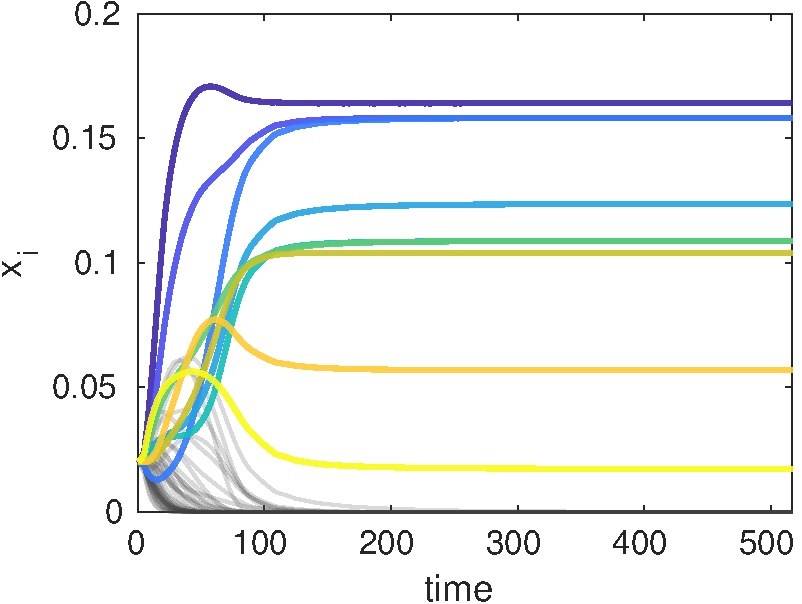
\includegraphics[width=0.7\textwidth]{figures/chp2/fig_3.pdf}
    \caption[Time evolution of mutualistic community]{Time evolution for a $50$-species mutualistic community of strength $\alpha_+ = 0.5$ in an ER graph with linking probability $p = 0.3$. At the end of the simulation, only $9$ species survive (in color), so persistence equals $18\%$.}
    \label{chp2:fig:3}
\end{figure}

The trajectories during the simulations are confined in the simplex and can settle in an equilibrium point. The equilibrium points of Eq.~(\ref{chp2:eq:replicator}) are obtained when $\dot{x}_i = 0, \, \, \forall i$. Two possible classes of solutions are found analytically: the origin (${x}^*_i = 0, \, \, \forall i$) and the values that satisfy:

\begin{equation}
    \sum_j \Lambda_{ij} x^*_j = \sum_{j,k} x^*_j \Lambda_{jk} x^*_k ,
\end{equation}
 which in turn, can be expressed as:
\begin{equation}
    \alpha_s \sum_{\substack{j \\ i\neq j} } A_{ij} x^*_j + c x^*_i = \alpha_s \sum_{\substack{j,k\\ j\neq k} } x^*_j A_{jk} x^*_k + c \sum_j x^{*2}_j
    \label{eq:solution}
\end{equation}

The equilibrium point depends on $\alpha_s$ and $c$, as well as the network structure encoded by $A$.  
If a solution has some extinct species (${x}^*_i = 0$) the right-hand side of Eq.~\eqref{eq:solution} can take any value, but it will involve $\alpha_s$, $c$, and $A$ too. Thus, as a result of describing communities as networks with embedded dynamics, the final state of a species depends on the parameters and the way in which species are connected. This setting is suitable because we want to understand how interaction patterns impact the ecological processes, eventually affecting whether or not species survive.\\

Moreover, environmental changes can alter species interactions \cite{Sun2022ExperimentalWetland,tabi2020species} and then our proxy for an environmental disruption is a global modification of the interaction strength's intensity. A community is supposed to be at its full persistence for the structures described in Subsection~\ref{chp2:2.1} for a set of interaction strength values. Then, an environmental change occurs and alters all interaction values to a new $\alpha_s$ but not the links between species. We start our simulations at that point with equal frequencies for all species and run the dynamics while tracking the species that go extinct  due to this change. Importantly, we do not remove by hand any species following the environmental change, but let the network structure affects the dynamics. We finish the simulations when a stationary state has been reached. 

\subsection{Structural Predictors: Network Metrics}  \label{chp2:2.3}

We aim to discover what are the structural characteristics that predict which species will survive. 
%In the language of complex networks, these structural characteristics are node metrics, that quantitatively capture intriguing aspects of network structure. \\

%We have chosen several candidates to test whether they are able to give us information about the survival of species.

There are many such measures, and our election has been made mainly among standard --but informative-- metrics, and structural indicators for food webs. 
%Despite it is well-known that food webs have  global structural properties that are different from those of non-trophic interaction networks \cite{Kefi2015NetworkShores,guimaraes2020structure}, the literature is biased toward food webs \cite{pascual2006ecological,kefi2020theoretical}. Since there aren't many examples of non-trophic interactions (but see \cite{Allesina2009GooglingCoextinctions, Morone2019TheEcosystems}), we also tested metrics originally associated with food webs in the hope that they might be helpful in our situation as well.\\
Since literature is biased toward food webs \cite{pascual2006ecological,kefi2020theoretical}, but see \cite{Allesina2009GooglingCoextinctions, Morone2019TheEcosystems}, we have included those predictors in our analysis despite the structural differences with non-trophic networks \cite{Kefi2015NetworkShores,guimaraes2020structure}.

Another point to consider is that species' self-regulation creates what is known in complex networks as a self-loop, a link that connects  a node to itself. Since all species have one self-loop, we have computed the metrics without taking them into account.\\

  In Table~\ref{chp:2:tab:nodeMetrics}, we present a short description where predictors are grouped together according to what structural aspect they stress. Some measures are related to the centrality of nodes, or to the analysis of groups of similar nodes within the network, and some others account for the different configurations of links.

\begin{table}[t]
\caption[Node metrics]{Node metrics. The complete list of measures with their definitions and references can be found in Appendix~ \ref{chp:methods:predictors}.}\label{chp:2:tab:nodeMetrics}
\begin{tabularx}{\textwidth}{XXX}
\hline
Centrality             & Meso-scale                              & Signed                            \\
\hline
\hline
Degree $k$             & k-core                                  & Strength                          \\
Betweenness centrality & Rich Club                               & Relative Interaction  Index (RII) \\
Closeness centrality   & Clustering Coefficient  (CC)            & Relative Balance  Index (RBI)     \\
Eigenvector centrality & Average neighbor degree  (Avg. Neig. k) & PN centrality                     \\
Pagerank               &                                         & Generalised PageRank  (GPR1)            \\
                       &                                         & Signed PageRank   (GPR2)  \\             
                       \hline
\end{tabularx}
\end{table}


\paragraph{Centrality metrics:} They describe a node's importance, i.e. its capacity to have an impact on other nodes in a network. There are several definitions of importance, so there are several descriptors \cite{Newman2010}. The simplest of all is just the number of links connected to a node, i.e. the degree $k$. If we want to take the importance of the node's connections into account, the eigenvector centrality gives a centrality score proportional to the centrality of the neighbors. In a variant called PageRank, the centrality of a node is primarily proportional to the centrality of the neighbors but divided by their degree.

 Alternative formulations of centrality are based on paths. For example, betweenness centrality measures to what extent a node is located on pathways between other nodes, and closeness centrality assumes that a central node has a low average distance from other nodes.

\paragraph{Meso-scale metrics:} Quasi-local properties provide an intermediate description level by grouping nodes. As with the concept of importance, here we also face different working definitions for \textit{groups}. The k-core is one of these  metrics \cite{Morone2019TheEcosystems}. It is a set of nodes where each is connected to at least $k$ others. 

When there are no genuine groups but rather certain ways in which nodes are connected, we can measure the clustering coefficient $CC$ or the average neighbor degree. The $CC$ quantifies the level of transitivity of a node as the fraction of the neighbors that are themselves neighbors.

\paragraph{Signed metrics:}Finally, some of these properties can be generalized to include information about the sign of the interactions involved. Since our main objective is to model communities with mutualistic and competitive interactions, a natural property of the nodes is the degree of each type of interaction. For example, the competitive degree $k_-$ is the number of species with which a species is competing. To also consider the magnitude of the interactions, we define the strength of a node as the sum of the interaction strengths of its links. Other more complex metrics have been borrowed from social sciences such as the PN centrality and two generalizations of the PageRank have been developed for this study.

\subsection{Metrics' importance: Decision Trees} \label{chp2:2.4}
A common but arduous challenge in network science is to relate the dynamics on a network with its structure \cite{Newman2010,Holme2021NetworksConsequences}. Here, we face that challenge because we seek properties (structure) that determine the fate of a species (dynamics). Among the aspects that involve both the dynamics and the network structure, some are more well-suited to be treated analytically --like stability-- and others that don't. Our research question falls in the latter case due to the complexity of ecological networks, and hence we need another approach to classify  surviving species according to their structural features and find the most relevant of those features. Fortunately, machine learning classifiers can do precisely that.  \\

We have used a machine learning algorithm called Decision Trees,  whose fundamentals are explained in Appendix~\ref{appen:DT}. Decision trees generate a set of rules to predict the correct class of an observation from a set of variables. The rules are nominal yes/no questions about the properties of the variables.  \\

In our particular case, the observations are species and the classes are their state at the equilibrium, which is ``Surviving'' or ``Extinct''. For each community, we train a decision tree with that information and the initial node metrics as the set variables (see yellow box in Figure~\ref{chp2:fig:1}a).  The decision tree discriminates which species survive according to the values of some of the metrics. A tree whose root node is the competitive degree $k_-$ is depicted in Figure~\ref{chp2:fig:2}. This toy tree classifies species only based on four different metrics: $k_-$, Relative Interaction Index ($RII$), PageRank, and betweenness centrality.  Each node of the tree checks the value of one metric. Having a particular species in mind, the first decision to be made is whether its $k_-$ exceeds $3$. If not, we follow the left branch, and we see that the tree classifies the species as ``surviving''. If, however, it is smaller than $3$, we follow the right branch to the next node. Here, the tree asks if the $RII$ of the species is smaller than $0.5$. In this way, we will navigate the tree until we land on the corresponding leave. \\

\begin{figure}[t]
    \centering
    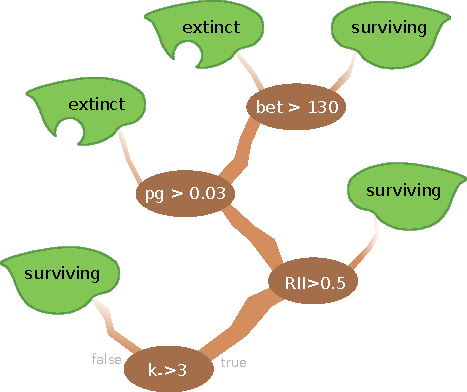
\includegraphics{figures/chp2/fig_2.pdf}
    \caption[Schematic diagram of a decision tree]{Schematic diagram of a decision tree. It has four nodes: competitive degree ($k_-$) as the root node, Relative Interaction Index ($RII$), PageRank ($pg$) and betweenness centrality ($bet$). These node metrics are the ones chosen during the training as the most useful to classify the species of an imaginary community. The threshold values are only for illustrative purposes.}
    \label{chp2:fig:2}
\end{figure}

To test the accuracy of the decision tree, we can cast a glance at the confusion matrix, which presents the percentage of correct and incorrect classifications (Figure~\ref{chp2:fig:6}a  as well as in Figure~\ref{chp2:fig:8}). For example, in Figure~\ref{chp2:fig:6}a, the decision tree for $\texttt{Emp}$\_$\texttt{IL}$ classifies with $99.5\%$ sensitivity that an extinct species actually goes extinct and with $99.2\%$ specificity that a surviving species will survive. False positives (extinct species predicted to survive) and false negatives (surviving species labeled as extinct) are very low, $0.5\%$ and $0.8\%$ respectively. \\

An accurate decision tree will find among all the proposed structural node properties the most relevant ones, which will be called \textit{structural predictors}. The importance profile (see e.g. Figures~\ref{chp2:fig:5}  and \ref{chp2:fig:7}) displays the quantitative importance of each potential predictor based on the definition of importance given by Eq.~\eqref{eq:importance}. The structural predictors stand out as the properties with systematically higher importance among the different structures. \\

Finally, to further test the generality of the predictors for each interaction type, we will modify some characteristics of the communities and train a decision tree for each new scenario. In particular, we will vary the interaction strength $\alpha$ (Figure~\ref{chp2:fig:4}), add noise to its value (Figure~\ref{chp2:fig:9}) and perform simulations with diverse network structures
%%%%%%%%%%%%%%%%%%%%%%%%%%%%%%%%%%%%%%%%%%%%%%%%%%%%%%%%%%%%%%%%%%%%%
\section{On the brick: results of structural predictors step by step}


%\paragraph{(moti+what)} First, we simulate communities with only one type of interaction as the first step towards combining  both competition and mutualism. Given that environmental changes alter species interactions \cite{Sun2022ExperimentalWetland}, and this in turn can cause extinctions, we start studying  how exactly the persistence varies with the strength of the interactions $\alpha$. 

Once the methodology and scope have been defined, we start to build intuition about the results we are going to find. We begin simulating communities with only one type of interaction as the first step towards combining both competition and mutualism. By doing so, we mirror the traditional approaches in which networks only describe one ecological process, and check if our results are consistent with the previous literature. The results obtained in this situation will help us to better understand the implications of taking several interactions simultaneously. 

\subsection{Persistence and interaction strength}
Given that environmental changes alter species interactions \cite{Sun2022ExperimentalWetland,tabi2020species}, and this, in turn, can cause extinctions, we start studying  how exactly the persistence varies with the strength of the interactions. More precisely, we increase the interaction strength as a proxy of the environmental change and record the species that perish. Since our dynamical model has few parameters by construction, we go ahead studying how persistence varies with the strength of interactions $\alpha_+$ on one side and  $\alpha_-$ on the other. We simulate communities for all the network structures of Section~\ref{chp2:2.1}, varying $\alpha_s$ by several orders of magnitude, and measuring the final percentage of surviving species. 
As a technical note, the artificial networks have been constructed in such a way that they have the same connectance as the empirical ones.  For the latter, we only take the links that correspond to the interaction type being studied. For example, if we focus on mutualism, the community of Figure~\ref{chp2:fig:1} will have solely green and gray links.\\

\begin{figure}[t!]
    \centering
    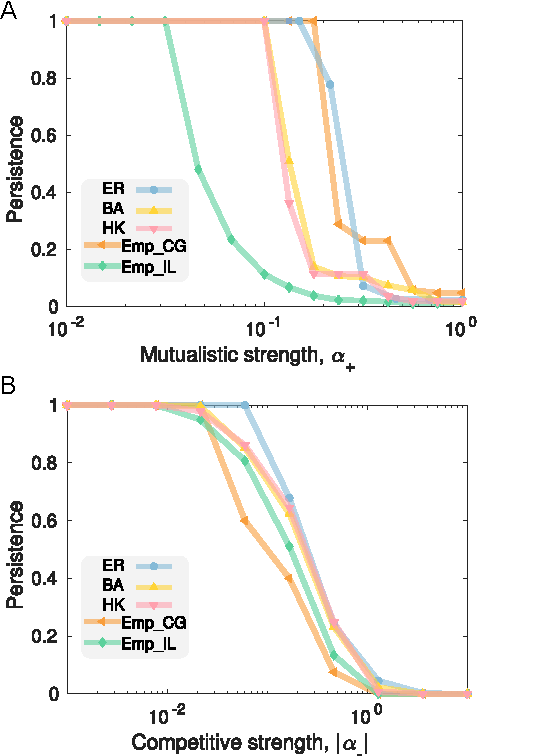
\includegraphics[width=0.6\textwidth]{figures/chp2/fig_4.pdf}
    \caption[Impact of interaction strength on persistence]{ Persistence decreases with high  interaction strength in absolute value for all network models. For illustrative purposes, only the largest empirical network of each type is displayed. Type (A) is represented by the pollinator network
 $\texttt{Emp}$\_$\texttt{IL}$ \cite{robertson1928flowers}. It has a total  of $n = 1500$ species, $456$ plants, and their $1044$ pollinators. Type (B) is $\texttt{Emp}$\_$\texttt{CG}$, a $104$ plant-species network extracted from \cite{Saiz2017EvidenceNetworks}. The random models have been simulated $10$ times for each value of $\alpha_s$, created  with $n = 500$ and a connectance $C$ equal to $\texttt{Emp}$\_$\texttt{IL}$ ($C_{mut} = 0.014$, $C_{com} = 0.012$). (Panel a) Mutualism. ER: $p =  0.009$; BA: $m_{links} = 2$; HK: $m_{links} = 2$, $p_t = 0.4$,  (Panel b) Competition. ER: $p =  0.1$; BA: $m_{links} = 30$; HK: $m_{links} = 30$, $p_t = 0.7$.}
    \label{chp2:fig:4}
\end{figure}

A smaller number of species survives as the absolute value of the interaction strength increases for both interactions and all network constructions, as shown in Figure~\ref{chp2:fig:4}. Networks simply differ in terms of when the transition happens, although  the critical value is rather similar. For instance, in Figure~\ref{chp2:fig:4}b, the lines for the BA and HK models are superimposed. This result falls into the traditional understanding of community ecology, where strong interactions lead to smaller or unstable communities \cite{May1972WillStable}, or smaller feasibility domains \cite{Grilli2017}. \\

After this result, we can assure that our proposed structures and dynamics work as expected and now proceed further to check the possible predictors. To do that, we choose an interaction strength that gives us a persistence of around $50\%$ to prevent biases in the training of the decision trees (see Section~\ref{chp2:2.4} and Appendix~\ref{appen:DT} for more insights about decision trees and  Appendix~\ref{SI:1} for cases where persistence is not equal to  $50\%$). \\

To understand the effects of multiple interactions within the same community, we start by studying mutualistic and competitive networks separately. In both cases, we set a network structure and measure the initial node properties for each species. After simulations reach the equilibrium, a decision tree is trained. It is fed with the node properties and a boolean variable that encodes whether the species is alive at the end of the simulation or not. Finally, we obtain the relative importance of those metrics in predicting survival, which is explained in Appendix~\ref{appen:DT}. \\

\subsection{Mutualistic networks}

For all network types with mutualistic interactions, the most important node property is eigenvector centrality, as can be seen in Figure~\ref{chp2:fig:5}a for artificial networks and in Figure~\ref{chp2:fig:5}b for empirical networks. Furthermore, the accuracy of the prediction is high as shown in the confusion matrix of Figure~\ref{chp2:fig:6}a. We can therefore conclude that the decision tree is well-trained, and we observe that it points to eigenvector centrality as the main predictor of extinction after an environmental change for mutualistic networks. \\

\begin{figure}
    \centering
    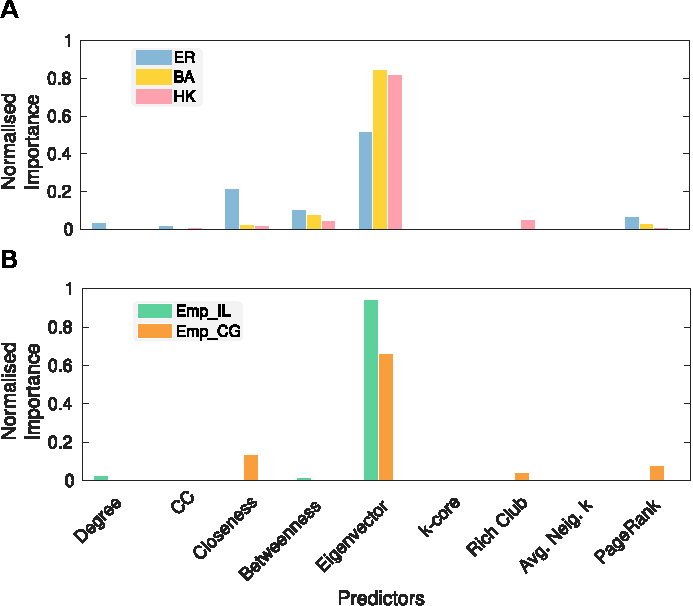
\includegraphics{figures/chp2/fig_7.pdf}
    \caption[Importance profile for mutualism]{When communities are purely mutualistic, the most important predictor for all network structures and interaction strengths is eigenvector centrality. The importance profile is in Panel a, where the normalized importance of each predictor  is plotted for artificial 500-node networks. ER: $p =  0.009$, $\alpha_+ = 0.22$; BA: $m_{links} = 2$, $\alpha_+ = 0.14$; HK: $m_{links} = 2$, $p_t = 0.4$, $\alpha_+ = 0.12$. (Panel b) Normalized importance for empirical networks from the three different datasets' collections. (type A) $\texttt{Emp}$\_$\texttt{IL}$: $N = 1500$, $\alpha_+ = 0.4$; (type B) $\texttt{Emp}$\_$\texttt{CG}$: $N = 104$, $\alpha_+ = 0.2$.}
    \label{chp2:fig:5}
\end{figure} 

Next, we plot the eigenvector centrality of the species at the beginning of the simulation versus their extinction time. We do this because the decision trees have determined that this type of centrality is the best one to classify whether a species becomes extinct. Eigenvector centrality is hence expected to correlate in a meaningful way with the fate of the species. From Figure~\ref{chp2:fig:6}b, we observe that the species that are worse connected, in terms of their eigenvector centrality, become extinct earlier. This tendency helps us to find the coherence behind the predictor, with the following narrative:

\begin{figure}[t]
    \centering
    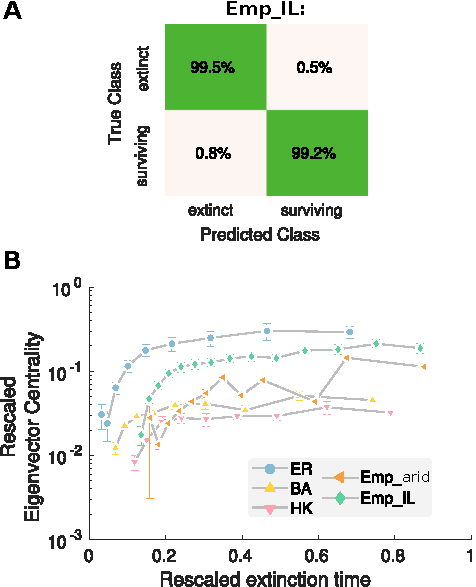
\includegraphics{figures/chp2/fig_6.pdf}
    \caption[Confusion matrix and time evolution of the eigenvector centrality in mutualistic communities]{(Panel a) The confusion matrix of one empirical network exemplifies the goodness of the trained Decision Trees. (Panel b) The initial eigenvector centrality plotted versus the time at which species become extinct reveals a pattern: species with low eig. centrality tend to die earlier. For clarity, the value for each point is the average eig. centrality of extinct species at nearby times. The same graph without binning is in Figure~\ref{chp2:fig:SI2_mut} of Appendix~\ref{appen:SuppPredictors}.}
    \label{chp2:fig:6}
\end{figure}

According to equation Eq.~(\ref{chp2:eq:replicator}), having more neighbors with positive $\alpha$ increases the local fitness and, consequently, we expect a centrality measure to take the main role in predicting survival. If a species has low eigenvector centrality, it is poorly connected and consequently has lower fitness. Moreover, eigenvector centrality grants a score proportional to the scores of the neighboring species, so a low value is an indicator that the mutualistic partners of the species are themselves performing badly. These species could not overcome the average fitness of the total community and hence become extinct. \\

Even for different types of networks, our result is in line with the literature and with what we expected. For instance, the fact that eigenvector centrality can rank the importance of species has already been found, but in the context of the collapse of food webs \cite{Allesina2009GooglingCoextinctions}. In mutualistic networks, there is still another reason that favors the role of centrality. One well-known property of these networks is their heterogeneity in the number of links: there are generalists and specialists species\cite{bascompte2003nested}. As a consequence, centrality metrics greatly vary among species and stand out as a distinctive characteristic. Moreover, although this structural regularity is reported for real-world networks, it is remarkable that the main predictor and the form of the curves in Figure~\ref{chp2:fig:6}b  are common to all types of structures, artificial as well as empirical. \\
 

\subsection{Competitive networks}
In this case, all the interaction strengths among species are negative. Taking a look at the mathematical form of local fitness in Eq.~\eqref{eq:localfitness}, a species with lots of competitors --more neighbors-- will have a lower fitness since the addends are negative. Thus, this causes its density to decrease faster. Accordingly, we expect again a centrality measure to play an important role in survival. \\

The trained decision tree reveals that the most important predictor, in this case, is  PageRank (Figure~\ref{chp2:fig:7}), again for both artificial (Panel a) and empirical networks (Panel b). The prediction has high accuracy too (Figure~\ref{chp2:fig:8}a).\\

Contrary to positive interactions, having high centrality is detrimental in competitive networks. And as a consequence, in Figure~\ref{chp2:fig:8}b, we observe that the species with  larger PageRank are the ones that became extinct first. Nevertheless, PageRank and eigenvector centrality are two very similar metrics, in the sense that both assign a score following the neighbors' centrality ratings \cite{Newman2010}. \\
 
\begin{figure}
    \centering
    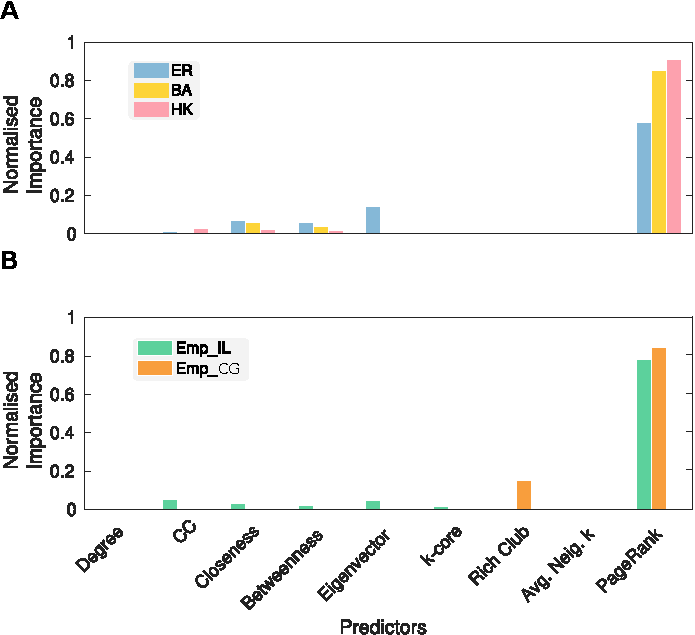
\includegraphics{figures/chp2/fig_5.pdf}
    \caption[Importance profile for competition]{In a community with only competition, the most important predictor for all network structures and interaction strengths is PageRank. The importance profile is in (Panel a), where the normalized importance of each predictor  is plotted for artificial 500-node networks. ER: $p =  0.009$, $\alpha_- = 0.45$; BA: $m_{links} = 2$, $\alpha_- = 0.4$; HK: $m_{links} = 2$, $p_t = 0.4$, $\alpha_- = 0.35$.  (Panel b) Normalized importance now for empirical networks from the three different datasets' collections: (type A) $\texttt{Emp}$\_$\texttt{IL}$: $N = 1500$, $\alpha_- = 0.25$; (type B) $\texttt{Emp}$\_$\texttt{arid}$: is the combination of all competitive networks in this collection because they were individually too small.}
    \label{chp2:fig:7}
\end{figure}

\begin{figure}
    \centering
    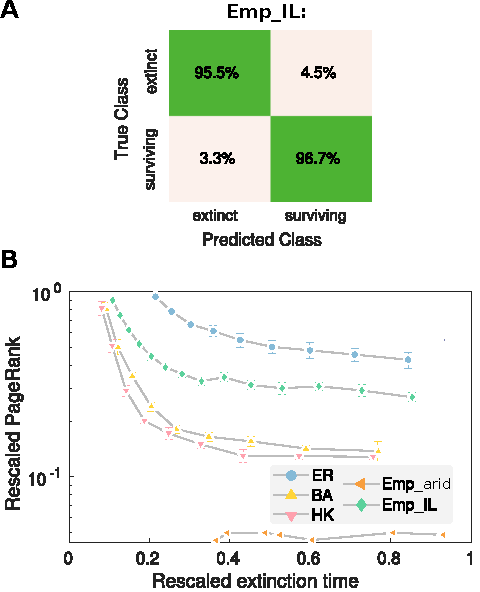
\includegraphics{figures/chp2/fig_8.pdf}
    \caption[Confusion matrix and time evolution of PageRank in competitive communities]{(Panel a) The confusion matrix of one empirical network exemplifies the goodness of the trained Decision Trees. (Panel b) The initial PageRank of each species plotted when it becomes extinct reveals a pattern: the species with high PageRank tend to die earlier. For clarity, the value for each point is the average Pagerank of species extinct at nearby times. The same graph without binning is in Figure~\ref{chp2:fig:SI2_comp} of Appendix~\ref{appen:SuppPredictors}. }
    \label{chp2:fig:8}
\end{figure}

Additionally, while the number of coexisting species varies with the intensity strength --the intensity of the environmental change--, the main predictors do not when only one interaction type is considered. The main predictors also remain the same when $\alpha_s$ is set as a baseline value plus some Gaussian noise, $\alpha'_s  = \alpha_s + \mathcal{N}(0,\sigma^2)$. In Figure~\ref{chp2:fig:9}, we can see that even when the noise has a standard deviation of the same magnitude as the strength itself, eigenvector centrality and  PageRank obtain the highest importance again. All these facts highlight the robustness of eigenvector centrality and PageRank as the main predictors for mutualistic and competitive networks, respectively. \\

\begin{figure}[t]
    \centering
    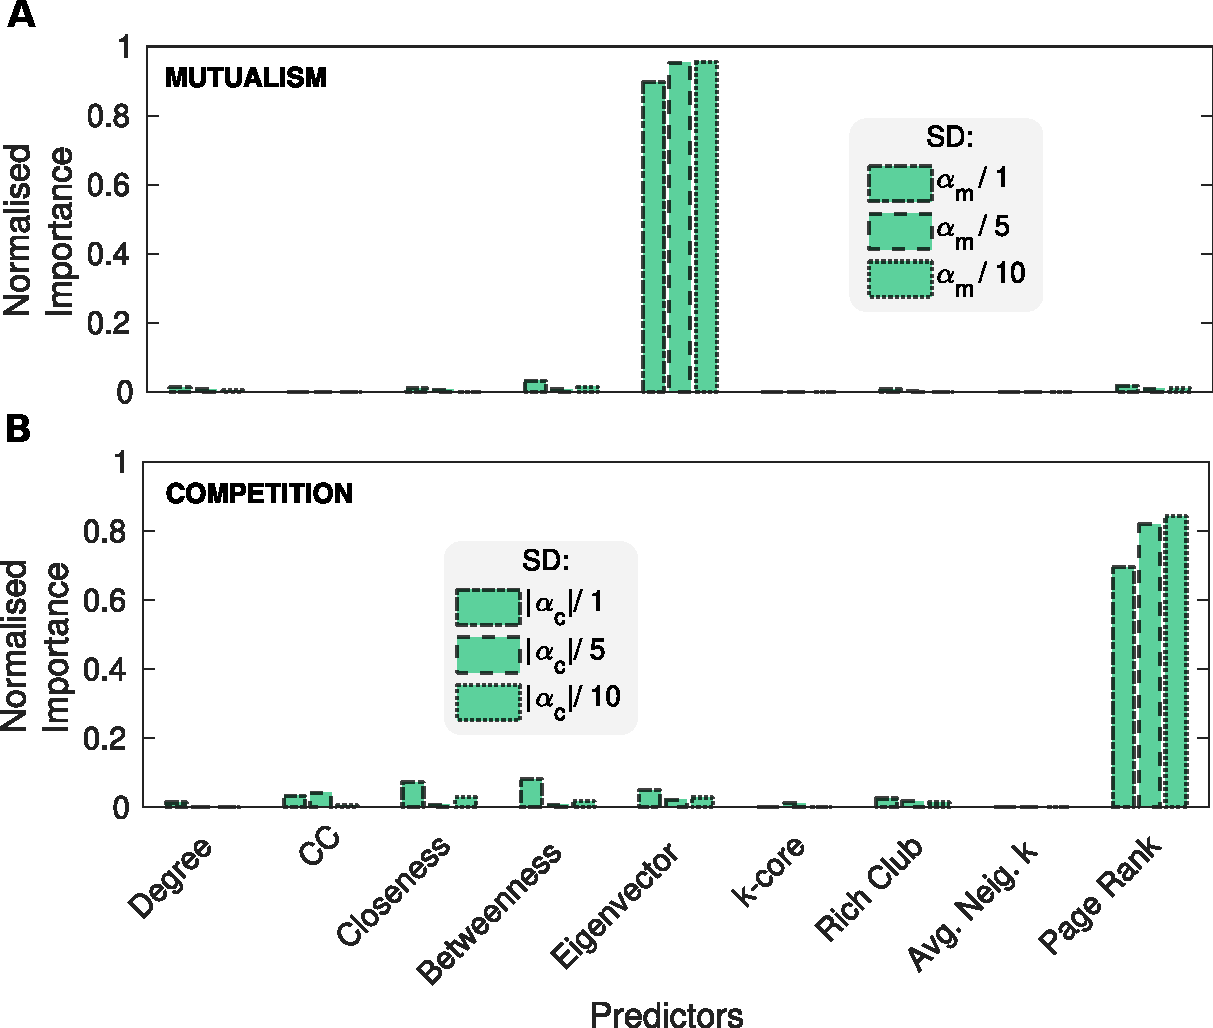
\includegraphics[width=\textwidth]{figures/chp2/fig_9.pdf}
    \caption[Importance profile with Gaussian noise]{The importance is not modified when we add Gaussian noise to the values of $\alpha$. SD stands for standard deviation. (Panel a) $\alpha_m = 0.04$ (Panel b) $\alpha_c = -0.2$. The network is $\texttt{Emp}$\_$\texttt{IL}$. }
    \label{chp2:fig:9}
\end{figure} 

 To summarize our results so far, we have studied one interaction type at a time after an environmental perturbation and, as a novelty, related the node properties of the species in the network with its final state after a simulation in simple dynamics, using a machine learning classifier. We have obtained that a single structural metric contains all the necessary information to predict whether a species will survive or not given its place on the network. This metric is eigenvector centrality for mutualistic networks, and PageRank for competitive networks. Importantly, these metrics continue to be the main predictors for different values and levels of noise of the interaction strength (i.e. of  persistence), and in all network structures that we have simulated. This suggests that the fate of the species depends heavily on their neighborhood and less on the overall network structure.
 
\subsection{Predictors in the presence of both types of interactions}\label{chp:2:3:4}

Once we have determined the predictors for only mutualistic or only competitive networks, we are ready to study communities with multiple interactions. We wonder whether the results for single-interaction communities hold, namely that solely one predictor is necessary to correctly classify the species, which in turn would be centrality-based and robust to changes in the intensity of interactions and network topology. In this case, we simulate communities with mutualistic and competitive interactions at the same time. \\

Adding a second type of interaction increases the complexity of the system, and so does the number of parameters to be chosen (number of mutualistic/competitive links, relative interaction strengths, etc).  We have thus introduced $\rho$, the ratio between competitive $\alpha_-$ and mutualistic $\alpha_+$ strength, to relate the interactions' strengths. Initially, it is set to $one$ to compare all the networks. For the same reason, we have only simulated real-world networks and not artificial ones. In that way, the percentage of positive and negative links in the networks and their distribution among species are based on empirical findings.\\

Comparing the effect of the real-world structure with a null model is now done via reshuffling (Section~\ref{chp:methods:networks}). We create alternative networks where overall characteristics such as the connectance and degree distribution of the empirical network are conserved, but the exact interacting patterns change at random. In that way, we could distinguish whether the future predictors depend on general average properties of the networks or on the particular way species connect. \\

The set of potential predictors is updated with signed metrics --as networks have now signed links. These metrics include information not only on structural properties but on the signs and strengths of the interactions (recall  Sections~\ref{chp2:2.3} and Appendix~\ref{chp:methods:predictors}). \\

Figure~\ref{chp2:fig:11} reveals the predictors obtained through the decision trees for our two types of empirical networks. There are several points at which the results of Figure~\ref{chp2:fig:11} differ from single-interaction networks. First notice that there is not a clear unique predictor. The highest importance is not as high as in the cases of only one type of interaction. Now we have other node properties that also have non-negligible importance. Regarding these properties,  they are mainly the metrics that take the sign of the interaction into account, especially PN centrality and PageRank's generalizations. Finally, and maybe this is the most intriguing of all the differences, the set of predictors varies from network to network. With two interactions, we lose the regularities found with just one interaction. Several metrics are needed to correctly classify species, whose identity and importance vary with the datasets. \\

\begin{figure}[t]
    \centering
    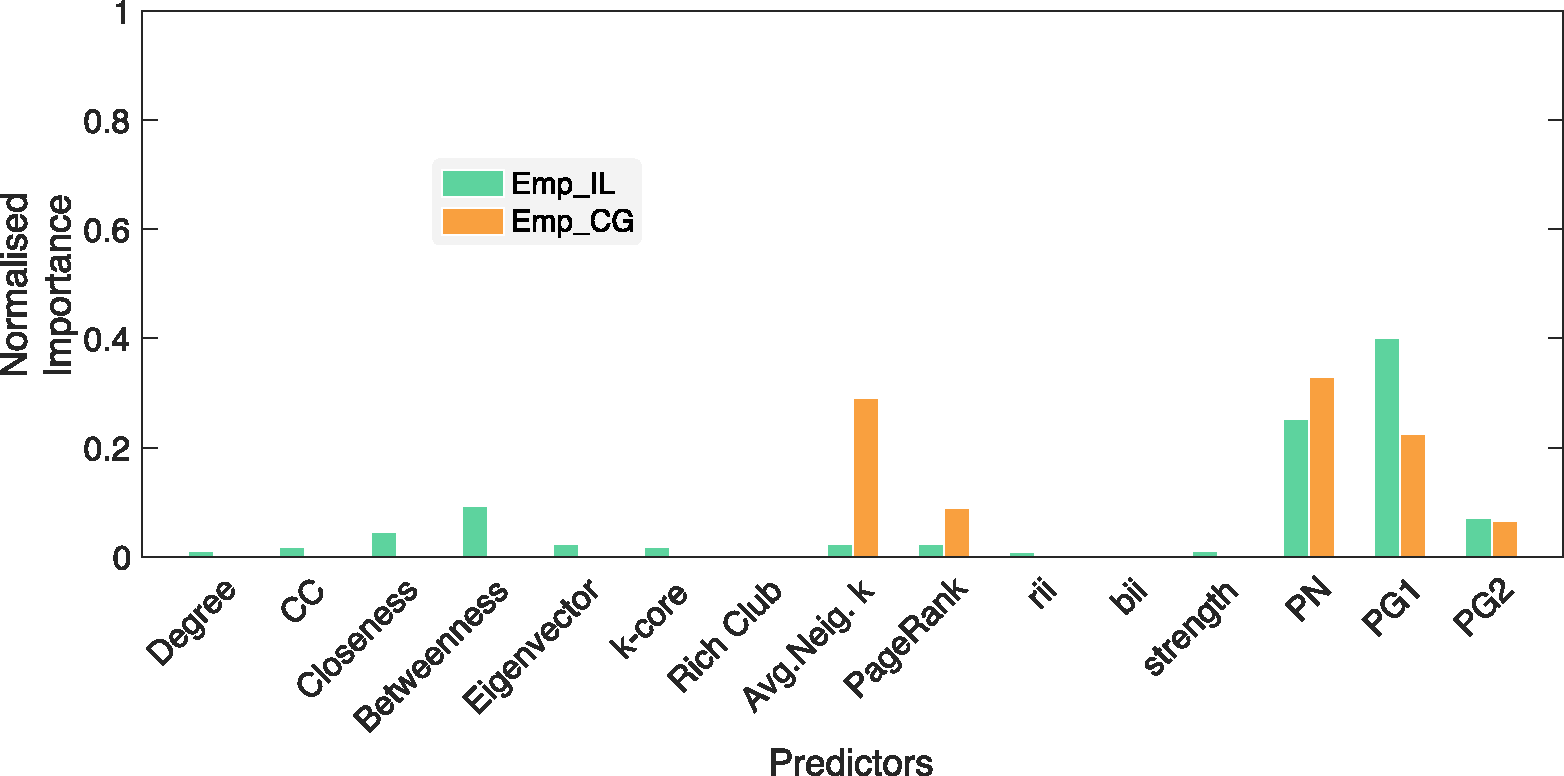
\includegraphics[width=1.05\textwidth]{figures/chp2/fig_11.pdf}
    \caption[Importance profile with several types of interactions at the same time]{The importance profile when mutualism and competition are studied simultaneously varies from network to network. For $\texttt{Emp}$\_$\texttt{IL}$ the parameters of the simulation are $\alpha_+ = \alpha_- = 0.14$ ($\rho = 1$). For $\texttt{Emp}$\_$\texttt{CG}$, $\alpha_+ = \alpha_-  = 0.18$ ($\rho = 1$).}
    \label{chp2:fig:11}
\end{figure}

To further examine the causes behind this divergence, we first explore the space of values of $\rho$ to test whether different strength ratios --and hence different environmental disruptions-- limit the range of predictors that are observed across different communities. Previously, the ratio had been set to one in Figure~\ref{chp2:fig:11} for simplicity, meaning that competition and mutualism have the same strength. We are interested in whether communities with a dominant interaction share similar predictors, which could suggest relative strength is a strong determinant of the predictors. Figure~\ref{chp2:fig:12} presents the importance profiles for several simulations of the same empirical network with different values of $\rho$, in particular when competition is five times stronger and weaker than mutualism. We observe that the set of predictors changes. Their importance is altered and even new predictors appear for some particular $\rho$ --a clear example is the closeness centrality for $\rho = 1/5$. Therefore, the predictors depend on the relative values of the interactions and, ultimately, this means that the internal dynamics embedded in the network affect them. \\

Then, we compare the importance profiles of our empirical networks with equivalent reshuffled networks maintaining the same interaction strengths. By confronting these random networks with the empirical ones, we can determine the role that interactions not placed at random have. Figure.~\ref{chp2:fig:13} shows that the predictors' importance changes and, given the error bars, the divergence can be large. Moreover, since the importance profile is not fully conserved after a notably conservative reshuffling, we can deduce that the predictors also depend to some extent on network structure. \\

\begin{figure}[t]
    \centering
    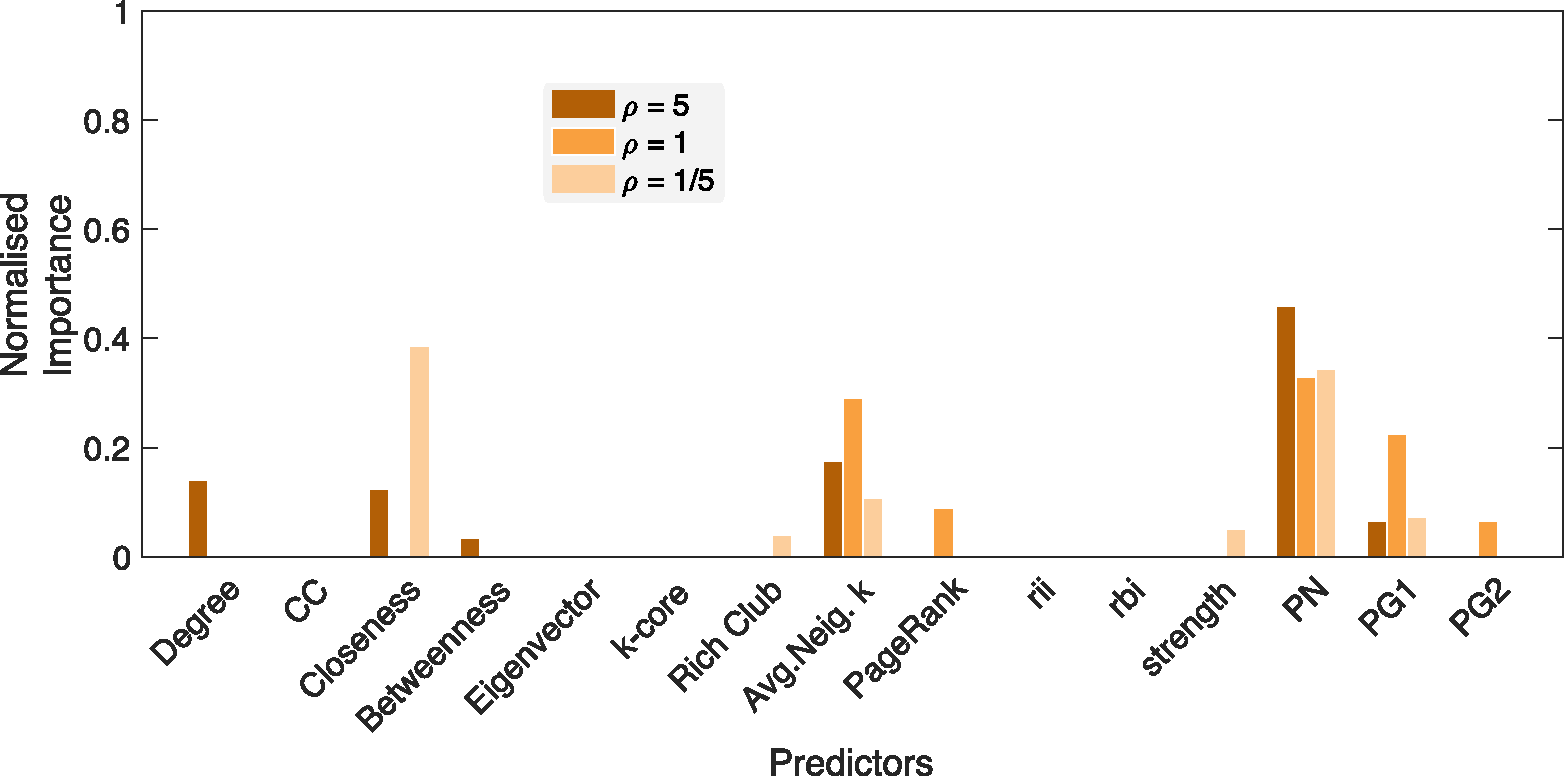
\includegraphics[width=1.05\textwidth]{figures/chp2/fig_12.pdf}
    \caption[Impact of the interaction strengths' ratio on the importance profile]{Changes on the importance profiles of the same network with different parameters. The system is $\texttt{Emp}$\_$\texttt{CG}$, where the setting for $\rho= 1$ is the same as in Figure~\ref{chp2:fig:11}. }
    \label{chp2:fig:12}
\end{figure}

 \begin{figure}[t]
    \centering
    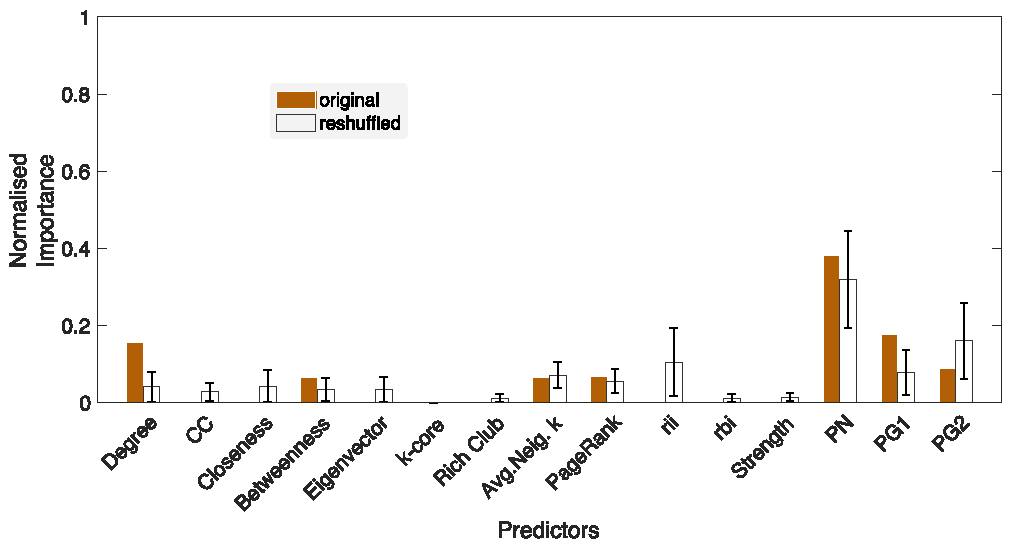
\includegraphics[width=1.05\textwidth]{figures/chp2/fig_13.pdf}
    \caption[Impact of reshuffling on the importance profile]{ Comparison between the importance profile of a network and their reshuffled versions. The importance of each predictor is averaged over $10$ reshuffled networks with the same dynamical parameters, and error bars mark the mean standard deviation. The original system is $\texttt{Emp}$\_$\texttt{CG}$ with $\rho = 5$ from Figure~\ref{chp2:fig:12}. }
    \label{chp2:fig:13}
\end{figure}

\begin{figure}
    \centering
    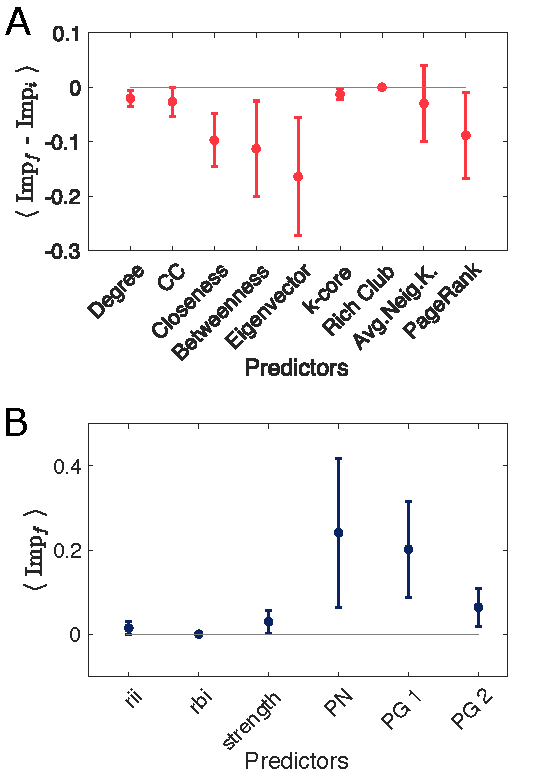
\includegraphics[width=.7\textwidth]{figures/chp2/fig_1415.pdf}
    \caption[ \, Differences on the importance for unsigned and signed predictors]{(Panel a) Average difference in importance for unsigned predictors before ($\texttt{Imp}_i$) and after  ($\texttt{Imp}_f$) adding signed metrics to the decision trees' training sets. The networks are the nine empirical networks described in \ref{tab:empnetworks}. (Panel b) Average importance of signed metrics over the same empirical networks. For all metrics, except average neighbors degree (Avg.Neigh.k.) in Panel a, the confidence intervals do not cross the horizontal axis. We can then conclude that the decrease in the importance of unsigned metrics as well as the non-zero importance of some signed metrics are significant.}
    \label{chp2:fig:1415}
\end{figure}

 We have just concluded that, when a system is described by more than one type of interaction, it cannot be characterized by a single predictor. The decision tree is not able to consistently find a main predictor for both interactions, even though it gets good results with the interactions in isolation. Worst still, one might think that \textit{the} important property is actually missing from the pool of potential predictors. Nevertheless, the sensitivity to the strength of interactions, and the fact that a given set of predictors varies with a subtle reshuffling suggest that there isn't any. \\

Eigenvector centrality and PageRank do not frequently appear as important when we study communities with both types of interactions. Instead, other metrics that record centrality influenced by the sign of the interactions become more relevant. The stability of communities cannot be predicted by simply adding what we already know from studying separately mutualism and competition. The combination of mutualistic and competitive interactions results in complex behavior. \\

The previous findings highlight the urgency of studying each community independently, as there is no robust, unique predictor. A particular distribution of interactions and their strengths seem to fix the important metrics, which change from case to case.   Nevertheless, we can still get some general results for multiple-interaction networks. \\

We can anticipate the most probable predictors because the signed metrics have appeared more frequently than other potential predictors, as it is seen in Figures~\ref{chp2:fig:11}, \ref{chp2:fig:12} and \ref{chp2:fig:13}. To strengthen this statement, we systematically average the importance of each predictor over all our empirical networks. We start by comparing the mean importance obtained by unsigned metrics before and after introducing signed metrics in the training set. The importance of the former decreases significantly (Figure~\ref{chp2:fig:1415}a) when signed metrics are also present in the training. Further, the mean importance of signed metrics is plotted in Figure~\ref{chp2:fig:1415}b. Several values are non-negative, indicating that they are important on average. Among them, PN centrality has the highest importance, followed by the generalizations of PageRank. These plots can be interpreted as follows: predictors based on the structure and dynamics of a system get higher importance because they contain more information about the fate of its species. A more complete knowledge of species dynamics is needed to evaluate species risks. Knowing only the structure is not enough.\\

The centrality of a species still plays a role, since  PN centrality and generalizations of PageRank are still based on how pivotal a species is. But being in some way central is not a sufficient indicator anymore. The number of mutualistic and competitive neighbors, and how strong these interactions are, also play a role. These two facts vary enormously among networks (see Table~\ref{tab:empnetworks}), preventing the decision tree from finding universal predictors.\\

\section{Discussion and perspectives} \label{chp2:4}

Protecting vulnerable species from extinction is crucial for conserving the planet. Apart from blatant cases, how to sort species in a community according to their extinction risk is an open problem. One fruitful approach is to make use of a network representation of the ecological relationships species participate in \cite{pascual2006ecological}. Traditionally, these networks describe only one type of interaction in isolation, and artificially remove species without modeling their abundances \cite{Sole2001}. Here, considering simple dynamics with both mutualism and competition, we have found that the regularity and predictability that hold for mutualism and competition when studied separately no longer apply. \\

We have started our work finding a node metric that predicts what species are going to become extinct first after an environmental change when only one type of interaction is present. Using a machine learning classifier, we have found that the species that survive in only mutualistic networks are the ones with the highest eigenvector centrality. We have obtained an equivalent result for only competitive communities, where species perish first if they have high values of PageRank. However, in ecological networks simultaneously including both interactions, species are no longer characterized by a local structural property. Including dynamical factors like the strength of their interactions enhances survival prediction. \\
%Furthermore, communities with more than one interaction are  described by a unique set of metrics. \\

A direct consequence of these results is that a species that was predicted to be thriving according to its mutualistic interactions may not be that safe. The predictors that determine safety vary when we add information on competitive interactions. In addition, we cannot ultimately anticipate the new set of predictors since they vary from network to network and with interaction strength.  And ultimately, we may not have complete information on the present interactions and their strengths --certainly not all of them. \\

This lack of universality contrasts with the regular patterns found when only one type of interaction is considered in our model and the literature. For example,  k-core is thought to be a predictor of structural collapse in mutualistic ecosystems \cite{Morone2019TheEcosystems}. Would this prediction change if competition was  added to the study? Seminal works have taught us that the architecture of ecological networks may be the result of the interweaving effect of several interactions. This is the case of the ubiquity of the nestedness, a main highlight of the architecture of mutualistic networks, that  minimizes competition and increases
biodiversity \cite{bastolla2009mutualism}.\\ 

 We have only studied mutualism and competition in the present work. The reason behind this choice is the proposed balance effect that the two interactions have on ecosystems \cite{bastolla2009mutualism,Wang2021InterspecificNetworks, Gracia-Lazaro2018TheEcosystems}. A natural question that arises is whether our results can be extended to communities with other interactions. Our methodology is ready to be applied to combinations of other kinds of non-trophic interactions such as parasitism \cite{dominguez2021structure, pilosof2017multilayer}, or in food webs \cite{Garcia-Callejas2018ThePersistence,Garcia-Callejas2021TheConstraints}.  \\

Finally, we have only presented here results that are oriented towards the prediction of survival after a change in parameters since that was our main objective. Still, the model has an interesting behavior by itself and calls for more systematic studies to unveil the interplay between structure and dynamics. For example, the impact of the ratio of interaction strengths on persistence, or how predictors change when the dynamics are refined to Lotka-Volterra equations with allometric coefficients. \\

% TO CONCLU: As a take-home message, when we study communities with both types of interactions, predictors are not universal and vary with the structure of each community and the interaction strengths. As a consequence of the results of this work, we are now in a position to highlight the significance of revisiting classic results of interactions in isolation, which bring us closer to the ultimate challenge of studying several interactions simultaneously to better understand ecosystems.

%Many efforts are made to allocate resources for conserving the planet. One approach is to protect certain species that are considered key players for the heath of an ecosystem. How to identify these species is, however, still far to be settled. An intuitive way to assign importance 
%Each community is unique. In addition, the importance of node characteristics depends not only on network structure, but on the strength and sign of the interactions. 


\part{Social systems feat.\ ecology}
\chapter{Quantifying the drivers behind collective attention in information ecosystems} \label{chp:3}

Explaining how humans behave when communicating online is crucial for our society. Unhealthy communication systems can give rise to echo chambers or fake news, which are alarming phenomena that, ultimately,  threaten the democratic discourse. Understanding the individual drivers behind collective attention  can help to maintain our information ecosystems healthy.  Various approaches have been proposed in recent years precisely to explain \textit{what} and \textit{how} drivers shape how our society processes information. From a data analytic perspective, several works have demonstrated the role of social interactions \cite{gonccalves2011modeling, romero2011influence, borge2011structural, omodei2015events}, competition in information diffusion \cite{weng2012competition, altman2013competition}, and the quality of the shared information  \cite{qiu2017limited}. These results have been supported by theoretical models, such as those for the emergence of echo-chambers \cite{baumann2020modeling} or the distribution of meme popularity \cite{gleeson2014competition, gleeson2016effects, asur2011trends}.\\

Here, we exploit the parallels between information and natural ecosystems to describe and quantify the main drivers of collective attention. Particularly, by analyzing diverse datasets from the online network Twitter and an ecological-based model, we can measure the intensity of the mutualistic and competitive interactions experienced by each actor, and how their values change when exogenous events captivate collective attention. We start by studying  the evolution of users' interests using topic modeling \cite{lancichinetti2011oslom}. In this way, we can calculate the similarity between memes (hashtags in Twitter) and users applying a concept inspired again by ecology (niche theory \cite{cai2021niches}). The niche similarity allows us to create interaction networks with both competitive and mutualistic terms, similar to ecological communities \cite{palazzi2021ecological}. We then analyze these networks to understand how the focus of collective attention around a few dominating topics can be interpreted as  deviations in the degree of mutualism and competition experienced by users. These analyses attribute the turns in attention to a reduction in the users' effective competition. Finally, we confirm this finding by replicating the interactions' changes observed in empirical data with simulations of an ecological-inspired model which proposes species abundance maximization as the main driver of collective attention.

%Explaining how humans behave when communicating online is crucial for our society. Unhealthy communication systems can give rise to echo chambers or fake news, which are alarming phenomena that, ultimately,  threaten the democratic discourse. Understanding the individual drivers behind collective attention  can help to maintain our information ecosystems healthy. Here, we investigate how competition for attention in online social networks and the user-adopted strategies to enhance visibility impact human communication. We based our study on a recently proposed parallelism between natural and information ecosystems \cite{plata2021neutral,palazzi2021ecological}. Specifically, by analyzing large datasets from the microblogging company Twitter and then carrying out numerical modeling of the system's dynamics, we manage to measure the level of competition for attention experienced by users and how it varies when external events capture collective attention. Our work extracts users' interests and memes' context from the data through topic modeling, and quantifies the strength of negative and positive interactions for users and memes using an ecological-inspired framework. It is based on ecological niche theory and bridges competition and mutualism with the interactions observed between the agents of the platform. Curiously, our findings reveal two distinct behaviors for memes and users during exogenous events. While the former suffers a boost in competition that can eventually lead to extinction, users experience a drop in effective competition as a result of the stronger impact of mutualistic interactions. Together, the two results explain the shift of collective attention toward specific topics. Finally, by developing a data-driven model of species dynamics, we are able to reproduce the observed shifts. This fact encourages an ecological approach to the study of information ecosystems since it provides fruitful tools for understanding  collective and social dynamics.\\

%The  work is developed throughout this Chapter, starting with the introduction of some particularities of the datasets employed in the analysis. We introduce step by step the technique of topic modeling  used to extract the information topics from online discussions, the methods to quantify the strength of mutualistic and competitive  interactions from the topics, and the ecologically-inspired model. Then, in Sections~\ref{chp3:2.1}, \ref{chp3:2.2} and \ref{chp3:2.3} we present our results for the time evolution of users' interests  and the user-hashtag interaction networks. Moreover, Section~\ref{chp3:2.4} confirms the previous results with numerical simulations. 

\section{Foundations for a model of information ecosystems}
\label{chp3:1}

\subsection{Twitter events datasets}
\label{chp3:1.1}

Since our scope is quantifying the switches in collective attention during exogenous events, we gathered  our data from Twitter, as the online microblogging platform is currently considered  an information and news source. And thus, users' activity will likely reflect events of different natures, from social and political affairs to natural disasters. This activity  can be recorded to track changes in users' interests and interactions. \\

We have analyzed three large datasets: the protests and events about the self-determination referendum coordinated by the government of Catalonia, Spain, in autumn 2014 \cite{palazzi2021ecological};  the April 2019 Spanish general elections \cite{palazzi2021ecological}; and the coverage of the earthquake that hit large parts of Nepal in 2015 \cite{zubiaga2018}. Table~\ref{chp3:tab:datasets} compiles the main features of the three datasets used in this Chapter. See Section~\ref{chp:methods:CSS} and Appendix~\ref{appen:DataCode} for a discussion on the details of their availability and the data collection process.  \\

\begin{table}
\caption[Main features of the three datasets]{\label{chp3:tab:datasets} Main features of the three datasets used in the study.}
\footnotesize
\begin{tabularx}{1\textwidth}{@{} X c c X X X}
\hline
Dataset&Starting date&Ending date & No.tweets & No.unique hashtags & No.unique users\\
\hline
\hline
Spanish Elections & \begin{tabular}{c}  20-04-2019  \end{tabular} & 04-05-2019 & 4882546 & 2952 & 41314 \\
\hline
Catalan Referendum & 01-09-2014 & 13-11-2014 & 220364 & 18116 & 78270 \\
\hline
Nepal Earthquake & 09-05-2015 & 18-05-2015 & 5641719 & 41589 &  1706559\\
%St. Patrick's Day & 15-03-2014 & 18-03-2014 & 829644 & 136684 & 615189\\
\hline
\end{tabularx}\\
\end{table}

 The datasets have been chosen because they represent a combination of unexpected and expected events \cite{lehmann2012dynamical,borge2016dynamics}: from a shocking natural disaster (Nepal's earthquake); to political/social issues, one of them constrained to a fixed timeline (Spanish elections) and the other being a combination of spontaneous protests and organized actions  (Catalan referendum). In particular, we limit the study to exogenous events, since we focus on how communication dynamics in online discussions are shaped by exceptional events.  Targeting events that interrupt the usual online social stream makes it possible to identify salient periods from the news and other media and to have a detailed view of their evolution. \\
 
We start the data preparation by only considering tweets with hashtags that have appeared a certain number of times. We restrict our analysis to hashtags posted at least $100$ times for the Nepal earthquake dataset as a result of its large size. For the political datasets, which are smaller, at least $75$ appearances were needed. Then, we consider, for each tweet, the anonymized ID of the user who posted it, the timestamp, and the list of all hashtags present in the tweet. With this information, we can use hashtags to discover users' interests and follow their evolution  through the entire discussion.  \\
\begin{figure}
   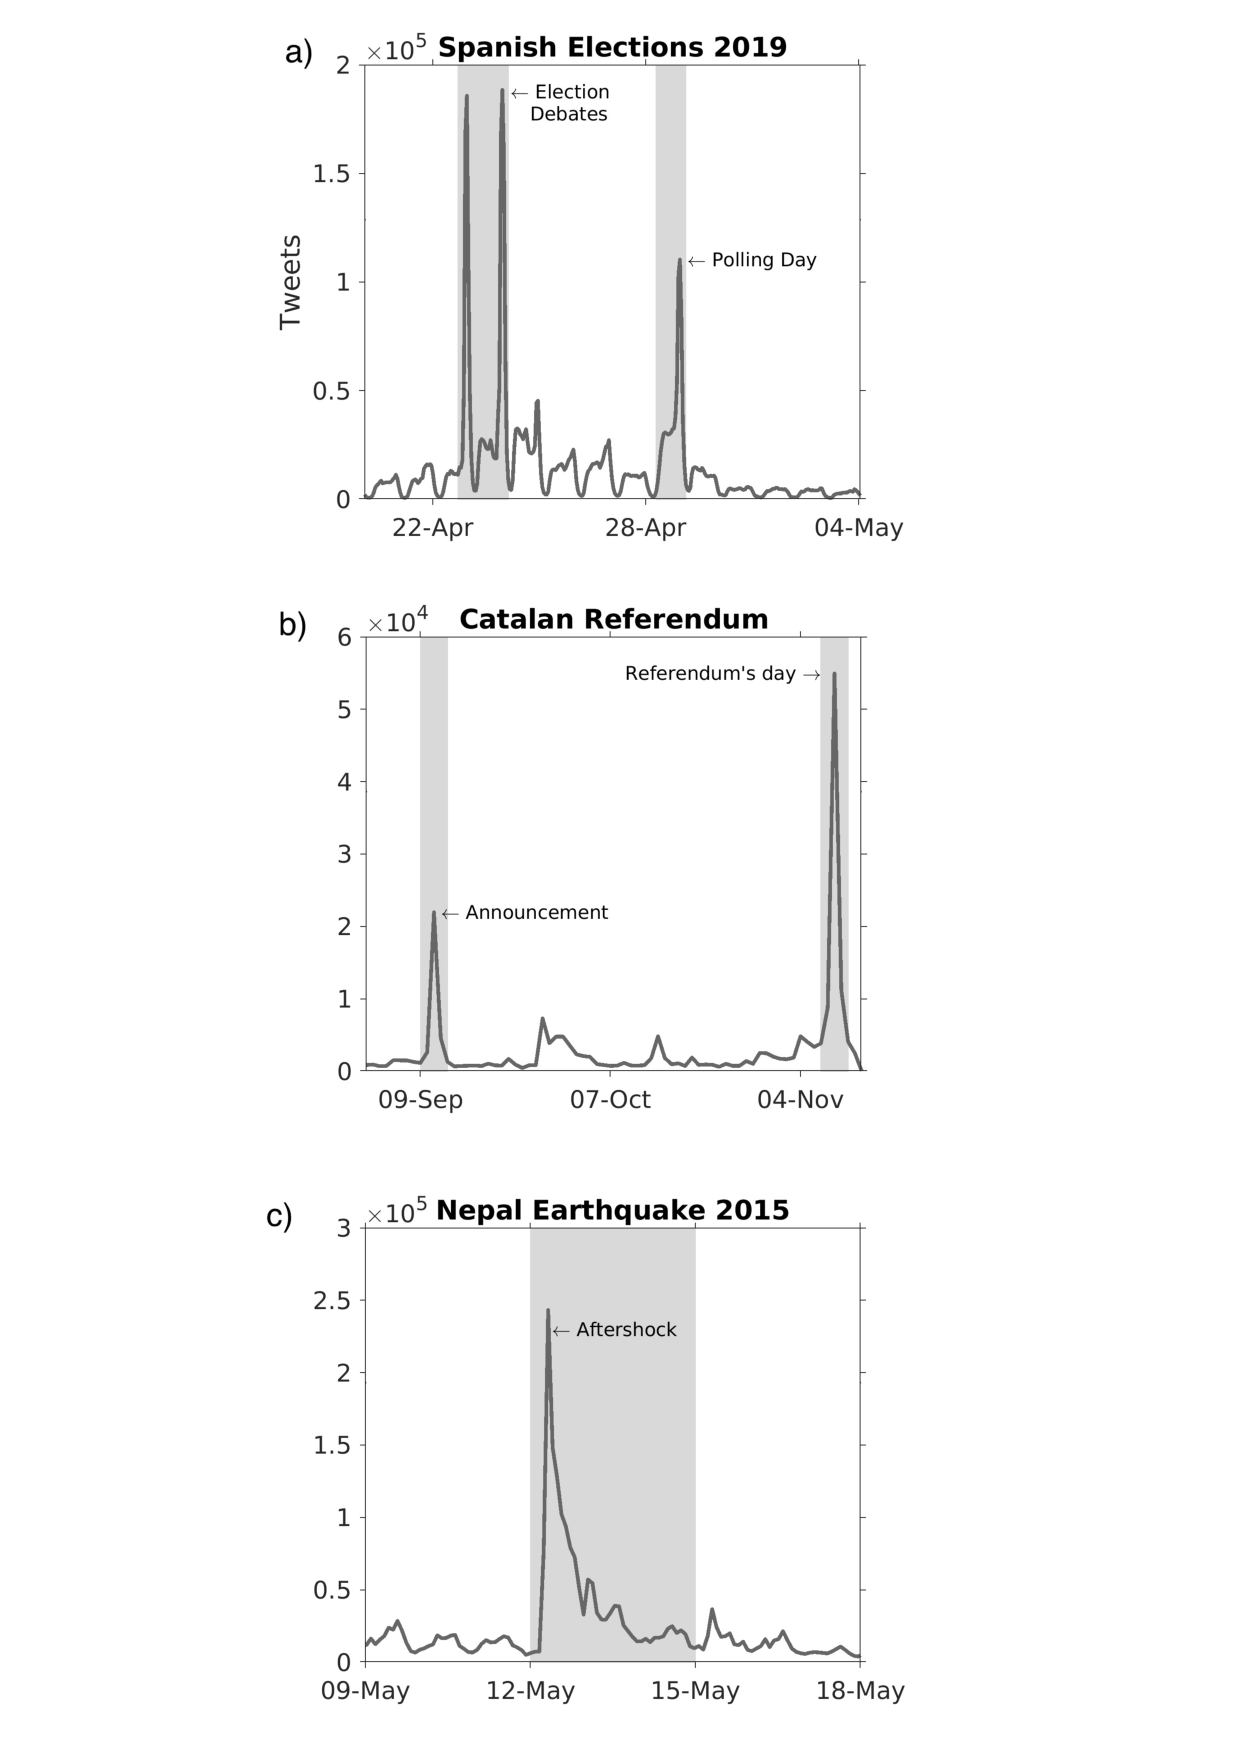
\includegraphics[width=1.05\textwidth]{figures/chp3/fig1new.pdf}

    \caption[Temporal evolution of the number of tweets]{Temporal evolution of the number of tweets for the considered datasets: the 2019 Spanish general elections (Panel a), the self-determination referendum in Catalonia in 2014 (Panel b), and the second major earthquake that hit Nepal in 2015 (Panel c). We highlight in gray the relevant events.
    }
   \label{chp3:fig:1}
\end{figure}

To capture the changes in attention, a methodology for extracting the topics being discussed during each interval must be developed, together with an intuition of competition and mutualism experienced by users in this techno-social context.  \\

\subsection{Information topics}
\label{chp3:1.2}

As the first step in deducing information topics from tweets, Figure~\ref{chp3:fig:1} shows the temporal evolution of the number of tweets for the datasets. All the datasets present clear high-activity periods related to external events, like the polling day for the Spanish elections (Figure~\ref{chp3:fig:1}a) or the referendum day for the Catalan Referendum (Figure~\ref{chp3:fig:1}b). These peaks in activity are surrounded by calmer periods characterized by much lower activity.  Since our aim is to study how competition for attention and users' interests vary between extraordinary and usual periods, we divide each dataset into different parts inspired by these different activities. More precisely,  for each dataset,  we determined the bulkiest spike in activity and set its duration as the size of the interval. In that way, we get intervals corresponding to ``peak'' and ``rest'' periods that are short enough to contain only a single event, along with having enough data during the calm periods. In the 2015 Nepal earthquake, the activity peak is $3$ day-long,  so we divided the dataset into intervals of precisely $3$ days. A similar reasoning was applied for the Catalan Referendum, where the extension of the largest spike is around $10$ days, and thus intervals are $10$ day-long. Yet,  since the Spanish elections dataset has a shorter duration, we set more irregular periods to guarantee enough tweets during the resting intervals.  \\

%This step is fundamental to measure the similarity between users and, eventually, quantifying the competition for attention that both users and memes experience over the development of the events.

Once we have defined the different periods, we focus on how to extract users' topics of interest from their tweets. To do so, we rely on a network theory approach developed precisely to infer information topics in Twitter \cite{weng2015topicality,cardoso2019topics,mussi2021topics}. It is based on hashtags co-occurrence, since users employ hashtags as keywords, to indicate the content of their message. Hashtags thus provide a straightforward representation of tweets' semantic context. If two or more hashtags appear in the same tweet, then it is safe to assume that there is a semantic association between them, as it usually happens to words frequently coinciding in texts \cite{turney2010words,martinez2011disentangling}. Based on this proxy,  we define information topics as cohesive clusters of hashtags that significantly appear together in tweets, capturing the commonalities in the hashtags' semantic context. From the perspective of the users, we assume that information topics will represent their set of interests. \\

The concrete methodology to determine topics is as follows: for each period considered in the data, if two hashtags appear in the same tweet, we connect them by a link, whose weight is proportional to the number of tweets where they co-occurred. To ensure that links only imply semantic associations between hashtags, we consider spurious and delete all the links whose weight is equal to or smaller than three. Once the weighted co-occurrence networks are built, we detect clusters of densely connected hashtags -- i.e. communities in the network science jargon-- and identify them as information topics. The communities in the different networks are detected using the OSLOM (Order Statistics Local Optimization Method) package \cite{lancichinetti2011oslom}, following the same procedure proposed in \cite{cardoso2019topics,mussi2021topics}. We choose OSLOM for community detection because it reveals overlapping communities, that is when nodes can belong simultaneously to more than one community. In this way, we guarantee that hashtags can have different meanings and hence be part of various topics. For example, four topics extracted from the Spanish elections dataset are depicted in Figure~\ref{chp3:fig:2} as wordclouds. They show  references to the most important dates, along with the names of several national parties. Some of these parties appear on more than one topic, indicating that they were present in several discussions. The combination of these words in each wordcloud makes clear that they represent different aspects of the discussion. For instance, the first wordcloud corresponds to election day and the third one revolves around the television electoral debate.\\
%Finally, extracting information topics for different periods will allows us to study how collective attention and the context of different memes evolves with the unfolding of the events.
\begin{figure}[t!]
    \centering
   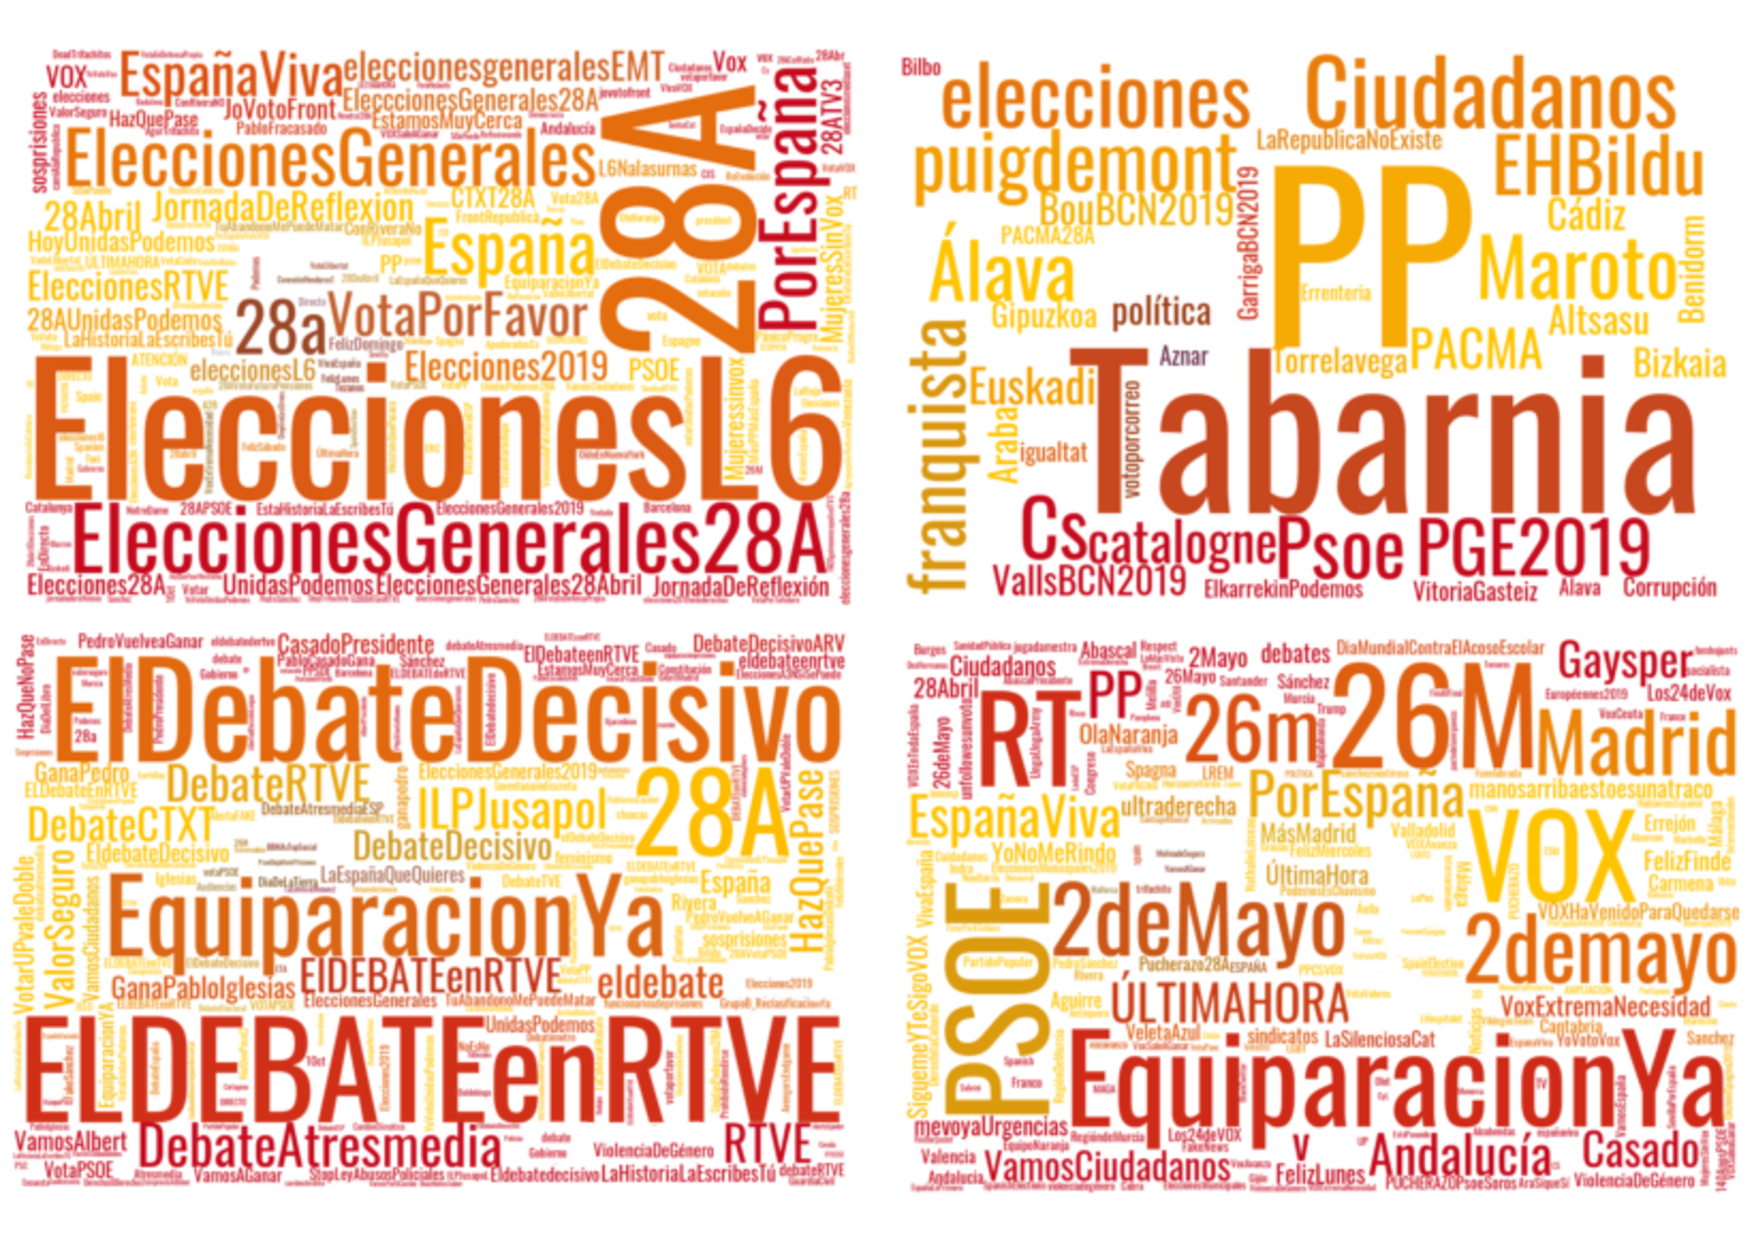
\includegraphics[width=1\textwidth]{figures/chp3/fig2.pdf}
   
    \caption[Word clouds of inferred topics]{Four example topics inferred from the Spanish general elections dataset. Each word cloud corresponds to one topic and it contains the most abundant hashtags, whose size is proportional to how many times they have been tweeted.}
   \label{chp3:fig:2}
\end{figure}

After obtaining the information topics from the data, we proceed to classify users into topics according to the hashtags they posted,
and ultimately,  to use the membership in various topics to detect users' interests. We proceed by building a feature vector $\mathbf{u}$ for each user, whose elements $u_i$ account for the number of occasions a hashtag belonging to topic $i$ was posted by the user. But since hashtags can belong to several topics within a period, the weight of each hashtag is split to take the number of communities they are part of into account. We assume one hashtag appearing only on one topic contributes to the corresponding entry of $\mathbf{u}$ by adding one. Conversely, a hashtag that is part of two topics $i$ and $j$  contributes $0.5$ to each $u_i$ and $u_j$. Finally, the value of $u_i$ is considered to be equivalent to the user's interest in topic $i$. The same method can be applied to build a counterpart hashtag vector $\mathbf{h}$ that quantifies their share of different topics.  In the diagrams of Figures~\ref{chp3:fig:3}a and \ref{chp3:fig:3}b we show a toy example of how vectors $\mathbf{u}$ and $\mathbf{h}$ are built. There, the hashtags posted by a user happen to be classified into three topics. One hashtag (\textit{\#lorem)} appears in topics $1$ and $2$ and therefore only adds $0.5$ to the corresponding entries $u_1$ and $u_2$. Likewise, its hashtag vector has a $1$ in the entries that correspond to topics $1$ and $2$. \\
 
A user vector quantifies how attention is scattered across different topics and how external events spotlight specific issues. In this sense, if information topics are thought of as ecological niches \cite{williams2000niche}, then $\mathbf{u}$ is the empirical equivalent of the niche profile proposed in \cite{cai2021niches,palazzi2021ecological} and introduced in Section~\ref{chp:methods:niche}. To build more intuition about this, let's define the ecological niche as ``the range of environmental conditions in which a population can persist'' \cite{hutchinson1957concluding}. Moreover, the niche profile of a species is formulated as the precise distribution of conditions in which that species thrives  \cite{williams2000niche}. For example, in Figure~\ref{chp3:fig:3}b, the user will prosper more in topic $3$ than in topic $1$. For cross-guild species (e.g., pollinators and plants), the niche proximity catches the complementarity of possible mutualistic partners. On the other side, within a guild, species with similar niches tend to share the same necessities (e.g., for nesting sites and light requirements). In that situation, the niche overlap instead captures competition for resources between species.\\

Returning to online social systems, information topics can be thought of as the environmental conditions in which users and hashtags thrive. individual interests may trigger competition too, and in this case, for attention. Users rival their peers for getting their posts read. In the same way, if an external event has focused attention on a specific theme, the hashtags related to it will suffer stronger competition for being chosen to appear on the users' screens. Lastly, users, aiming to reach potentially larger audiences, choose between hashtags when posting about popular content, leading to a kind of mutualistic interaction. Returning to our example, the user will benefit from posting hashtag \textit{\#lorem} again because it is very aligned with their interests, but posting a hashtag belonging to a hypothetical $4$\textit{th} topic would be zero since it is out of their scope. \\
\begin{figure}
   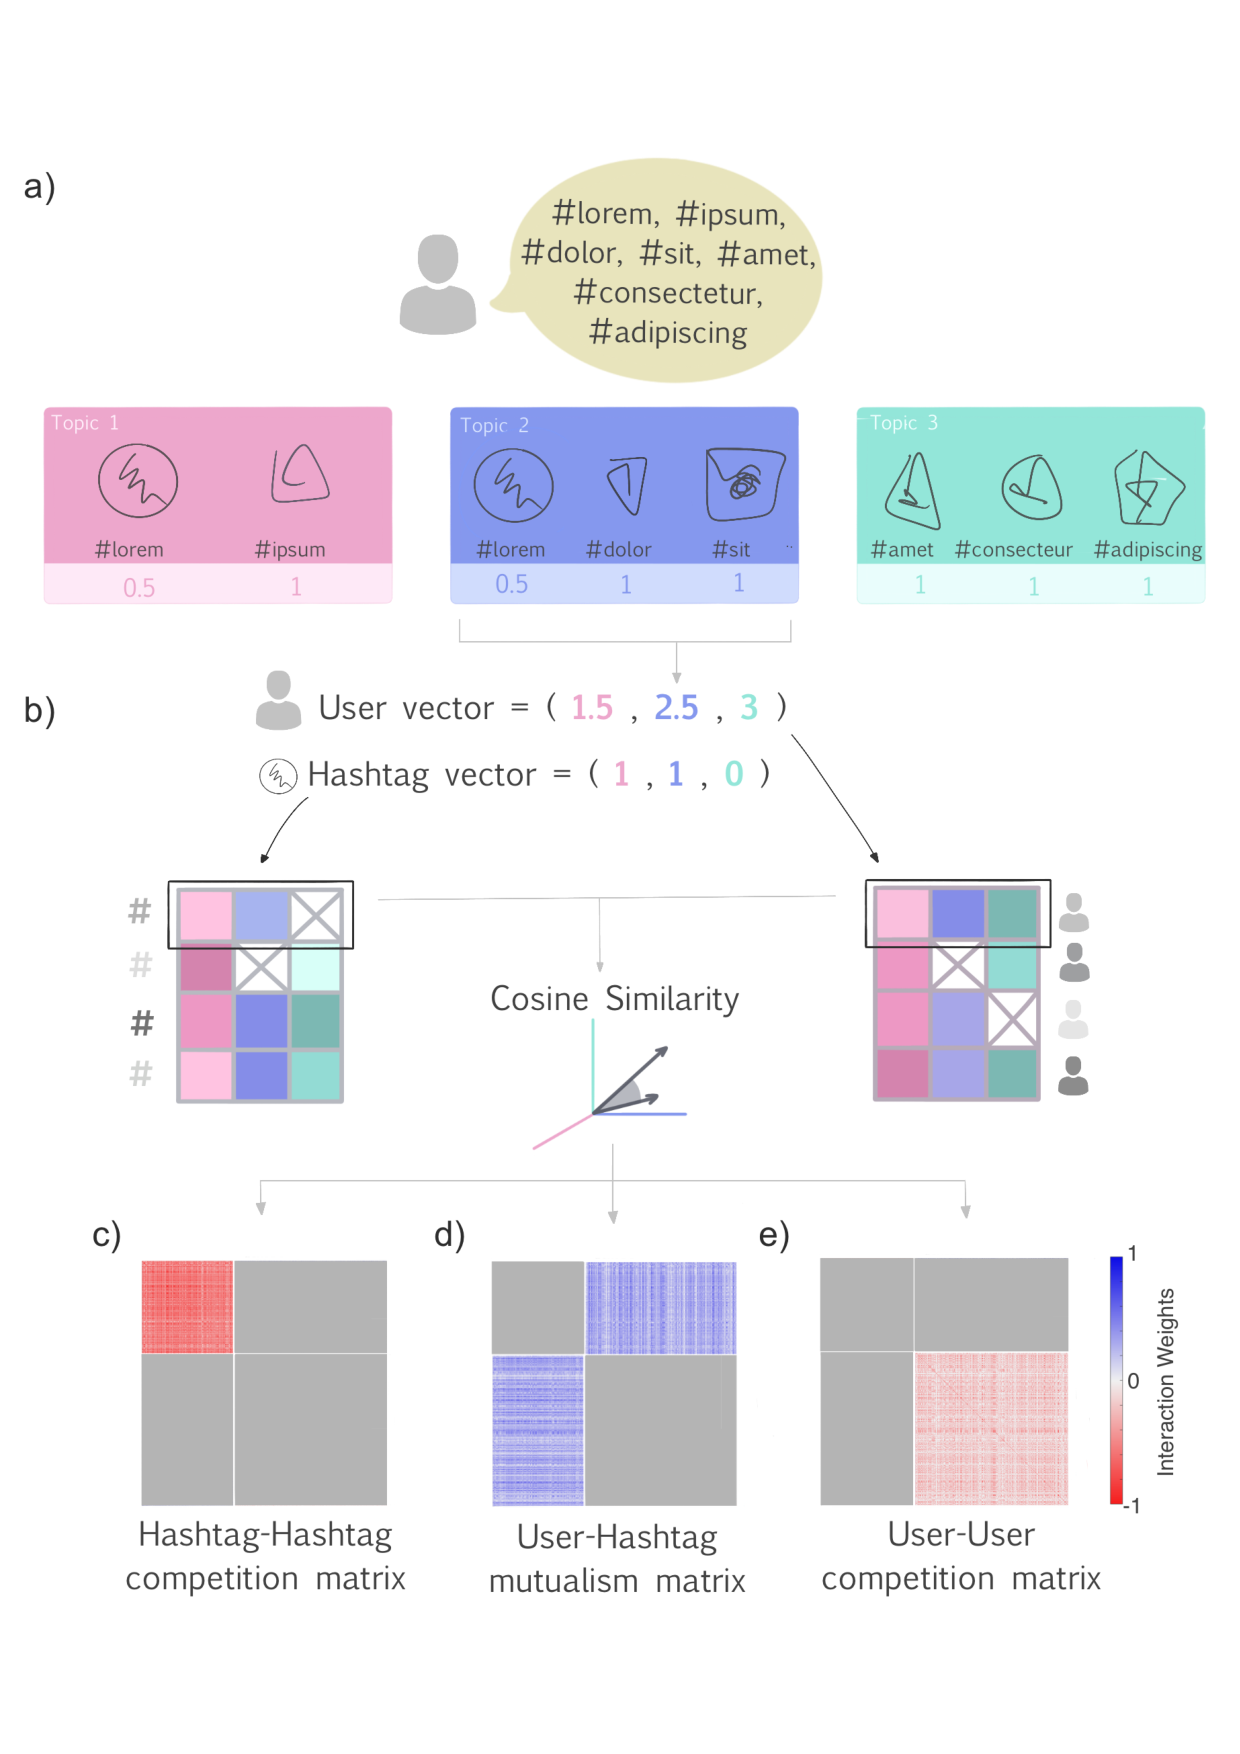
\includegraphics[width=0.95\textwidth]{figures/chp3/fig3.pdf}
    \centering
   
    \caption[Methodology for extracting user-topic and hashtag-topic vectors]{Illustration of the methodology for extracting user-topic and hashtag-topic vectors, and ultimately creating the competitive and mutualistic matrices. (Panel a) Using the algorithm proposed in \cite{cardoso2019topics}, hashtags are classified into topics. (Panel b) Hashtag-topic vectors encode the membership of each hashtag to one or more topics, so their dimension is the number of topics obtained. When a hashtag is part of more than one topic its weight is evenly divided between all the topics it belongs to. User-topic vectors are calculated from the hashtags tweeted by each user.  (Panels c, d, and e) The cosine similarity of each pair of user and hashtag vectors is tantamount to topic overlap. (Panels c and e) The elements of the hashtag-hashtag (user-user) competition matrices are computed proportionally to the topic similarity between hashtags (users). (Panel d) Similarly, the mutualism matrix is built as the similarity between hashtags and users. }
   \label{chp3:fig:3}
\end{figure}

To quantify the amount of competition users endure every period in the datasets, we calculate how similar $\mathbf{u}$ vectors are between users. For each pair of user vectors $\mathbf{u}$ and $\mathbf{v}$ we measure, inspired by the concept of niche overlap, their cosine  similarity: 

\begin{equation}
    sim_{cos}(u,v) = \frac{\mathbf{u} \cdot \mathbf{v}}{\left\Vert \mathbf{u} \right\Vert  \left\Vert  \mathbf{v} \right\Vert}.
\label{eqsim}
\end{equation}

In this way, we define a measure that goes from $0$ (where users have totally disconnected interests) to $1$ (perfectly aligned users). On the other side, hashtag competition can also be calculated likewise, using hashtag vectors $\mathbf{h}$ instead of $\mathbf{u}$ (see Section~\ref{chp3:1.4} for more details).  \\

Ultimately, to quantify how much mutualism a pair of a user $\mathbf{u}$ and hashtag $\mathbf{h}$ experiences, we also measure the cosine similarity:

\begin{equation}
    sim_{cos}(u,h) = \frac{\mathbf{u} \cdot \mathbf{h}}{\left\Vert \mathbf{u} \right\Vert  \left\Vert  \mathbf{h} \right\Vert}.
\end{equation}

We obtain, like for competition, $0$ similarity for pairs of users and hashtags without any topic in common, and a maximum of $1$ for totally aligned pairs.

\subsection{Dynamical model of users' attention}
\label{chp3:1.3}
Once developed a method to classify users and hashtags according to their interests, we can  use their similarities to measure how much competition and mutualism is experienced by each agent. Furthermore, to get an additional understanding of the driving mechanism behind changes in collective attention, we also utilize an ecology-inspired visibility optimization model \cite{palazzi2021ecological}, proposed to explain the structural shifts in the user-hashtag interaction networks through an event. \\

Following the analogies between information ecosystems \cite{palazzi2021ecological,plata2021neutral} and ecological communities, the model is based on an adaptive niche model \cite{cai2021niches}. Its main assumption is that the relations among species adaptively change to maximize the abundance of single species \cite{suweis2013emergence}. For information ecosystems, an optimization process where users seek to maximize their visibility is supposed to drive the attention dynamics. Hashtags and users are interpreted as species of a mutualistic community from two separate guilds --e.g., pollinators and plants in natural ecosystems. Competitive interactions occur between within-guild species (between hashtag-hashtag and user-user pairs), while mutualism takes place between species of different guilds (user-hashtag). Species dynamics follows Lotka-Volterra equations with a Holling-Type II functional response (see Section~\ref{chp:methods:LV}): 

\begin{equation}
\label{eq:dyn}
{\begin{aligned}{\frac {dn_i^U}{dt}}&=n_i^U \left(\rho_i^U - \sum_j \beta_{ij}^{UU}n_j^U + \frac{\sum_k \gamma_{ik}^{UH}n_k^H }{1+ h \sum_l \theta_{il}n_l^H} \right), \\[6pt]
{\frac {dn_k^H}{dt}}&=n_k^H \left(\rho_k^H - \sum_l \beta_{kl}^{HH}n_l^H + \frac{\sum_i \gamma_{ki}^{HU}n_i^U }{1+ h \sum_j \theta_{kj}n_j^U} \right).
\end{aligned}}
\end{equation}
where $n_i^U$ and $n_k^H$ represent the abundance (visibility) of species belonging to the users' ($U$)  or hashtags' ($H$) guild, $\rho_i^U$ and $\rho_k^H$ stand for their respective growth rates, while  $h$ is the handling time of the Holling-Type II mutualistic functional response. Matrices $\boldsymbol{\beta^{UU}}$, $\boldsymbol{\beta^{HH}}$ and $\boldsymbol{\gamma^{UH}}$ encode the strength of users' and hashtags' competitive and mutualistic interactions, respectively. Finally, $\boldsymbol{\theta}$ is the adjacency matrix of the bipartite network. An element $\theta_{ik}^{UH}$ equals one whenever user $i$ is employing hashtag $k$ in their posts. \\

The optimization process works as proposed in \cite{suweis2013emergence}, where users change their mutualistic connections to randomly selected hashtags, and the new rewiring is kept if and only if it induces an increase in abundance (a.k.a. visibility). Otherwise, the initial link is re-established (check Figure~\ref{fig:nicheModel}). At fixed time intervals, we randomly choose a user $i$, and rewire one of its current connections to a new random hashtag $l$. The link to rewire is selected with a probability $p_{il} \propto 1 - 1/k^{H}_{l}$ where $k^{H}_{l}$ is the  number of users connecting with hashtag $l$. This ensures that every hashtag has at least one mutualistic interaction. After the rewiring, we let the system evolve until it reaches a new equilibrium. If at this point the user $i$'s abundance is larger than before the rewiring, the new link is kept; otherwise, we restored the previous configuration.   \\

It should be noted that, in our model, only users are the active agents in the optimization process since they choose what hashtags to tweet to maximize their abundance (the proxy for visibility). Therefore, the changes in hashtags' connections are solely due to users' actions.  \\

\subsection{Estimating competition and mutualism from data}
\label{chp3:1.4}
Finally, we estimate the matrices of interaction strength among species ($\boldsymbol{\beta^{UU}}$, $\boldsymbol{\beta^{HH}}$ and $\boldsymbol{\gamma^{UH}}$) from our data following the approach proposed by Williams and Martinez \cite{williams2000niche}. 
Mutualistic and competitive strengths are proportional to niche overlap between species of the opposite (mutualism) and the same (competition) guilds. As introduced in Section~\ref{chp3:1.2}, the niche overlap $G_{ij}^{gg'}$ between species $i$ from guild $g$ and species $j$ from guild $g'$ is estimated as the cosine similarity between the topic vectors of $i$ and $j$. For the competition, the elements of the matrices $\beta_{ij}^{HH}$ and $\beta_{kl}^{UU}$ are simply proportional to the niche overlap by a global factor $\Omega_c$ that tunes the absolute interaction strength: $\beta_{kl}^{HH} \propto \Omega_c \cdot G_{kl}^{HH}$ and $\beta_{ij}^{UU} \propto \Omega_c \cdot G_{ij}^{UU}$. Correspondingly, the elements of the mutualistic matrix are defined as  $\gamma_{ik}^{UH} \propto \Omega_m \cdot G_{ik}^{UH}$. For the particular case of mutualism, the interaction strength matrix $\gamma_{ik}^{UH}$ is multiplied by $\theta_{ik}$ to incorporate the fact that user $i$ may not ($\theta_{ik}=0$) or may ($\theta_{ik}=1$) interact with hashtag $k$. Lastly, to compare the two strengths, and without losing generality, we set $\Omega_c = \Omega_m$. 


\section{The rise and fall of buzz: visibility optimization drivers collective attention}
\label{chp3:2}

Our analyses start by splitting our three datasets into different periods based on their activity (i.e., the total number of tweets produced), and following the approach explained in Section~\ref{chp3:1.2}. The objective of this division is to distinguish what we define as peak periods from resting periods. Peak periods are exogenous events that produce large activity on Twitter, such as the referendum day for the Catalan dataset or the TV debate for the Spanish elections. On the other side, during rest periods, the discussion is still happening but not driven by major external events. We will use the calmer periods to set a baseline for activity and collective attention and to contrast them with peak periods.  \\

\begin{figure}[t]
   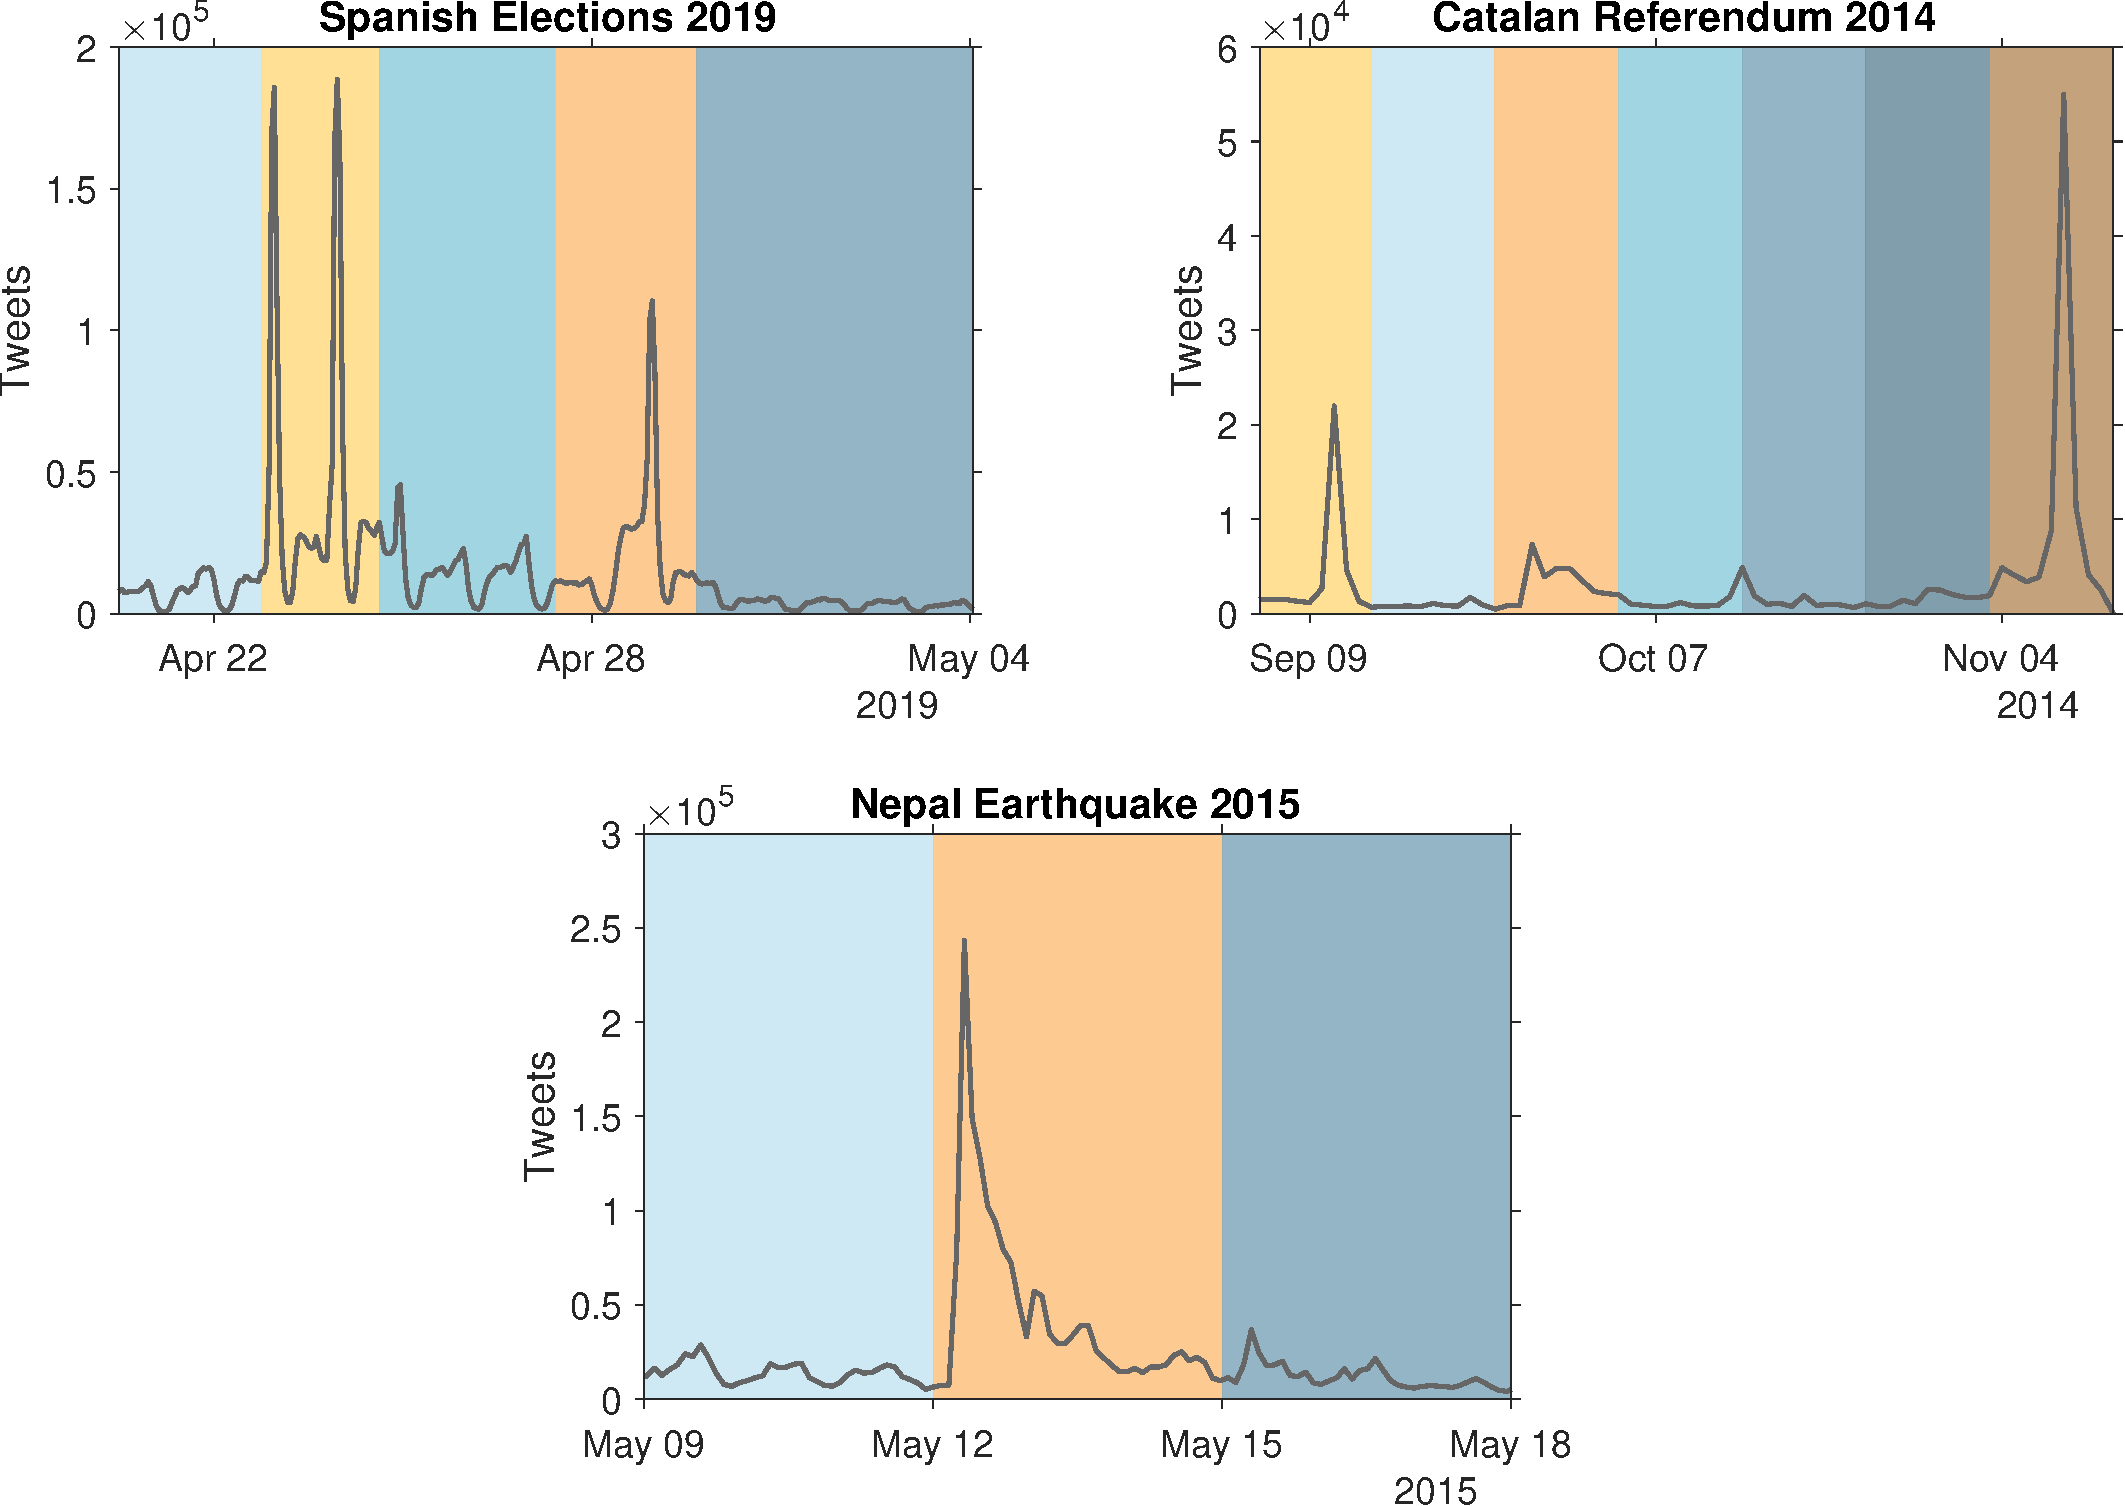
\includegraphics[width=1\textwidth]{figures/chp3/fig4a.pdf}
   
    \caption[Time evolution of the number of tweets by activity periods]{(Panels a-c) Time evolution of the number of tweets in the different datasets divided by activity periods. The colors of each period are just for visualization purposes.}
   \label{chp3:fig:4a}
\end{figure}

\begin{figure}
   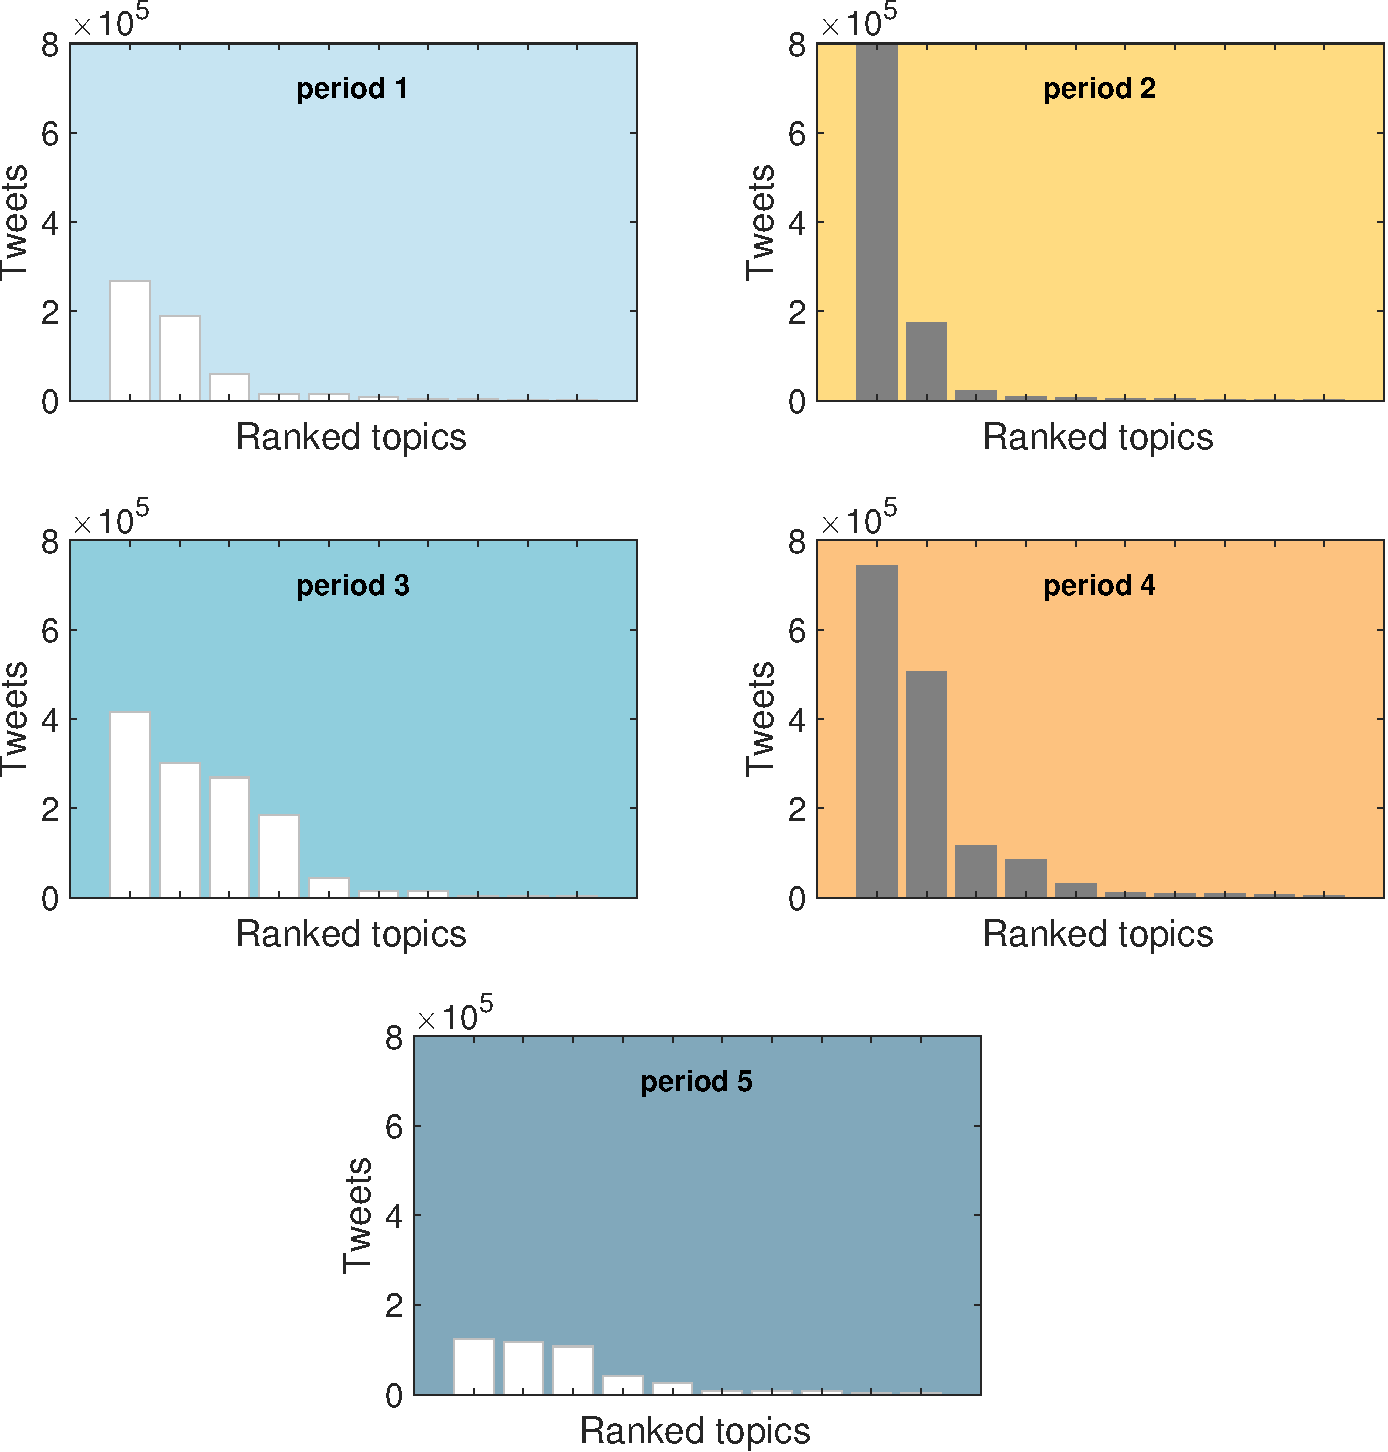
\includegraphics[width=1\textwidth]{figures/chp3/fig4b.pdf}
   
    \caption[Activity distribution through topics and periods]{(Activity (number of tweets) in the largest $10$ topics for every period of the Spanish elections dataset. Gray bars mark the peak periods.}
   \label{chp3:fig:4b}
\end{figure}
Figures~\ref{chp3:fig:4a}a-c illustrate the divisions of our datasets. For the 2109 Spanish elections dataset (Figure~\ref{chp3:fig:4a}a) we identify $5$ periods, where the second and fourth cover the main large events, while the fifth represents our baseline of activity. The third period is a combination of high activity and calmer times since it has smaller events taking place. In the 2104 Catalan referendum dataset (Figure~\ref{chp3:fig:4a}b), we identify $7$  different periods: the second, fourth, fifth, and sixth as resting states; and the first, third, and seventh as peaks. Finally, in the 2015 Nepal earthquake dataset (Figure~\ref{chp3:fig:4a}c), we define just three periods, with the first one representing the baseline state, the second period being the peak, and the third one a mixture of peak and rest.  \\

\subsection{Topics evolution}\label{chp:3:topicsevol}
\label{chp3:2.1}
Once specified our active and baseline intervals, we extract the topics of every period to study how the hashtag networks and users' interests evolve through time. Following the procedure described in  Section~\ref{chp3:1.2}, we create a hashtag co-occurrence network for each period and get the most important communities from it, which define our topics. \\

From the hashtag co-occurrence networks, we can study how topics evolve period by period, and how external events reorganize the corresponding discussions. Table~\ref{tab:nets}  summarizes the main features of the networks extracted from each considered dataset. A result that stands out is that although networks of different periods have different sizes, the number of topics (i.e. communities in the networks) is almost constant.  For example, the number of hashtags (i.e. nodes) in the Spanish elections dataset increases a $44\%$ between the most and least active periods --it varies from $1313$ to $1899$--  but the number of topics in each period only goes up by a $28\%$ --it ranges from $77$ to $60$. This fact deviates from our hypothesis that collective attention focuses on one or not many ``main topics'' during external events. However, considering not only the number of topics but also their activity, this discrepancy is solved. In Figure~\ref{chp3:fig:4b}, for the Spanish elections dataset, we show how activity --in terms of the number of tweets the topics generate-- distributes among the $10$ largest topics for the different periods. We can observe that activity, in general, is highly heterogeneous. However, during high-activity periods (plots with gray bars), this tendency intensifies with one or two topics gathering almost the $90\%$ of the tweets together. We get similar results for the other datasets, not shown in Figure~\ref{chp3:fig:4b}.  \\

\begin{table}
    \centering
\caption[Summary of the co-occurrence networks obtained from each dataset]{\label{tab:nets} Summary of the co-occurrence networks obtained from each dataset.}
\footnotesize
\begin{tabular}{c c c c c c }
\hline
Dataset & Period & No. hashtags & No. links & No. topics\\
\hline \hline
%Spanish & & & &\\
Spa. Elec. & 1 & 1344 & 6866 & 75 \\
& 2 & 1714 & 11587 & 68 \\
& 3 & 1899 & 12026 & 77\\
& 4 & 1736 & 12373 & 63\\
& 5 & 1313 & 5114 & 60\\

\hline

%Catalan Ref & & & &\\
Cat. Ref. & 1 & 703 & 3170 & 9 \\
& 2 & 310 & 863 & 20 \\
& 3 & 586 & 2070 & 10\\
& 4 & 350 & 1037 & 21\\
& 5 & 338 & 911 & 16\\
& 6 & 362 & 1112 & 13\\
& 7 & 1602 & 5837 & 12\\

\hline
%Nepal & & & &\\
Nepal & 1 & 471 & 1564 & 29 \\
& 2 & 771 & 4739 & 27 \\
& 3 & 670 & 2921 & 33\\

\hline

\end{tabular}\\
\end{table}


\begin{figure}[t]

    \centering
   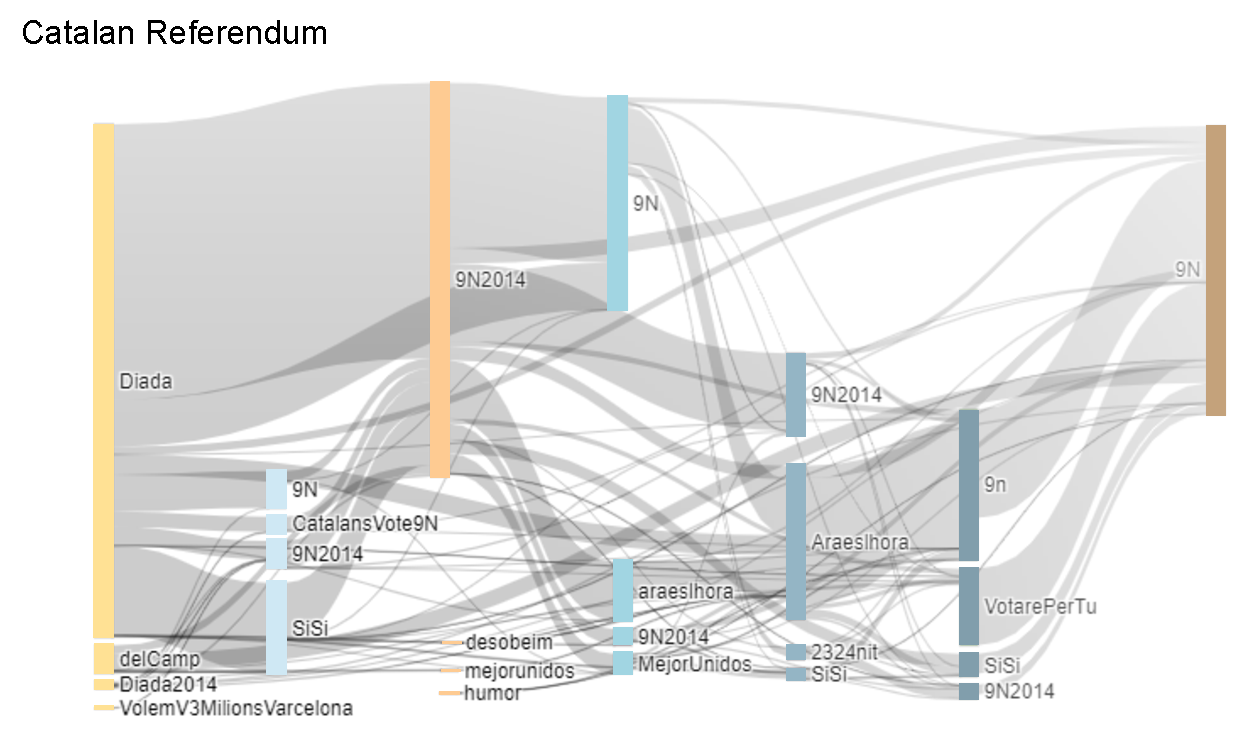
\includegraphics[width=1.05\textwidth]{figures/chp3/fig5.pdf}
   
    \caption[Alluvial diagram of topic sizes]{Topics' development for the Catalan referendum dataset is illustrated with an alluvial diagram. Boxes represent topics (communities in the co-occurrence network). Their colors encode the different periods, and their sizes are proportional to the number of tweets that belong to each topic. To ensure readability visibility, only the four largest topics are shown for each period. Flows represent the volume of tweets moving from one topic in a certain period to another topic in successive periods.}
   \label{chp3:fig:5}
\end{figure}

\begin{figure}[t]
    \centering
   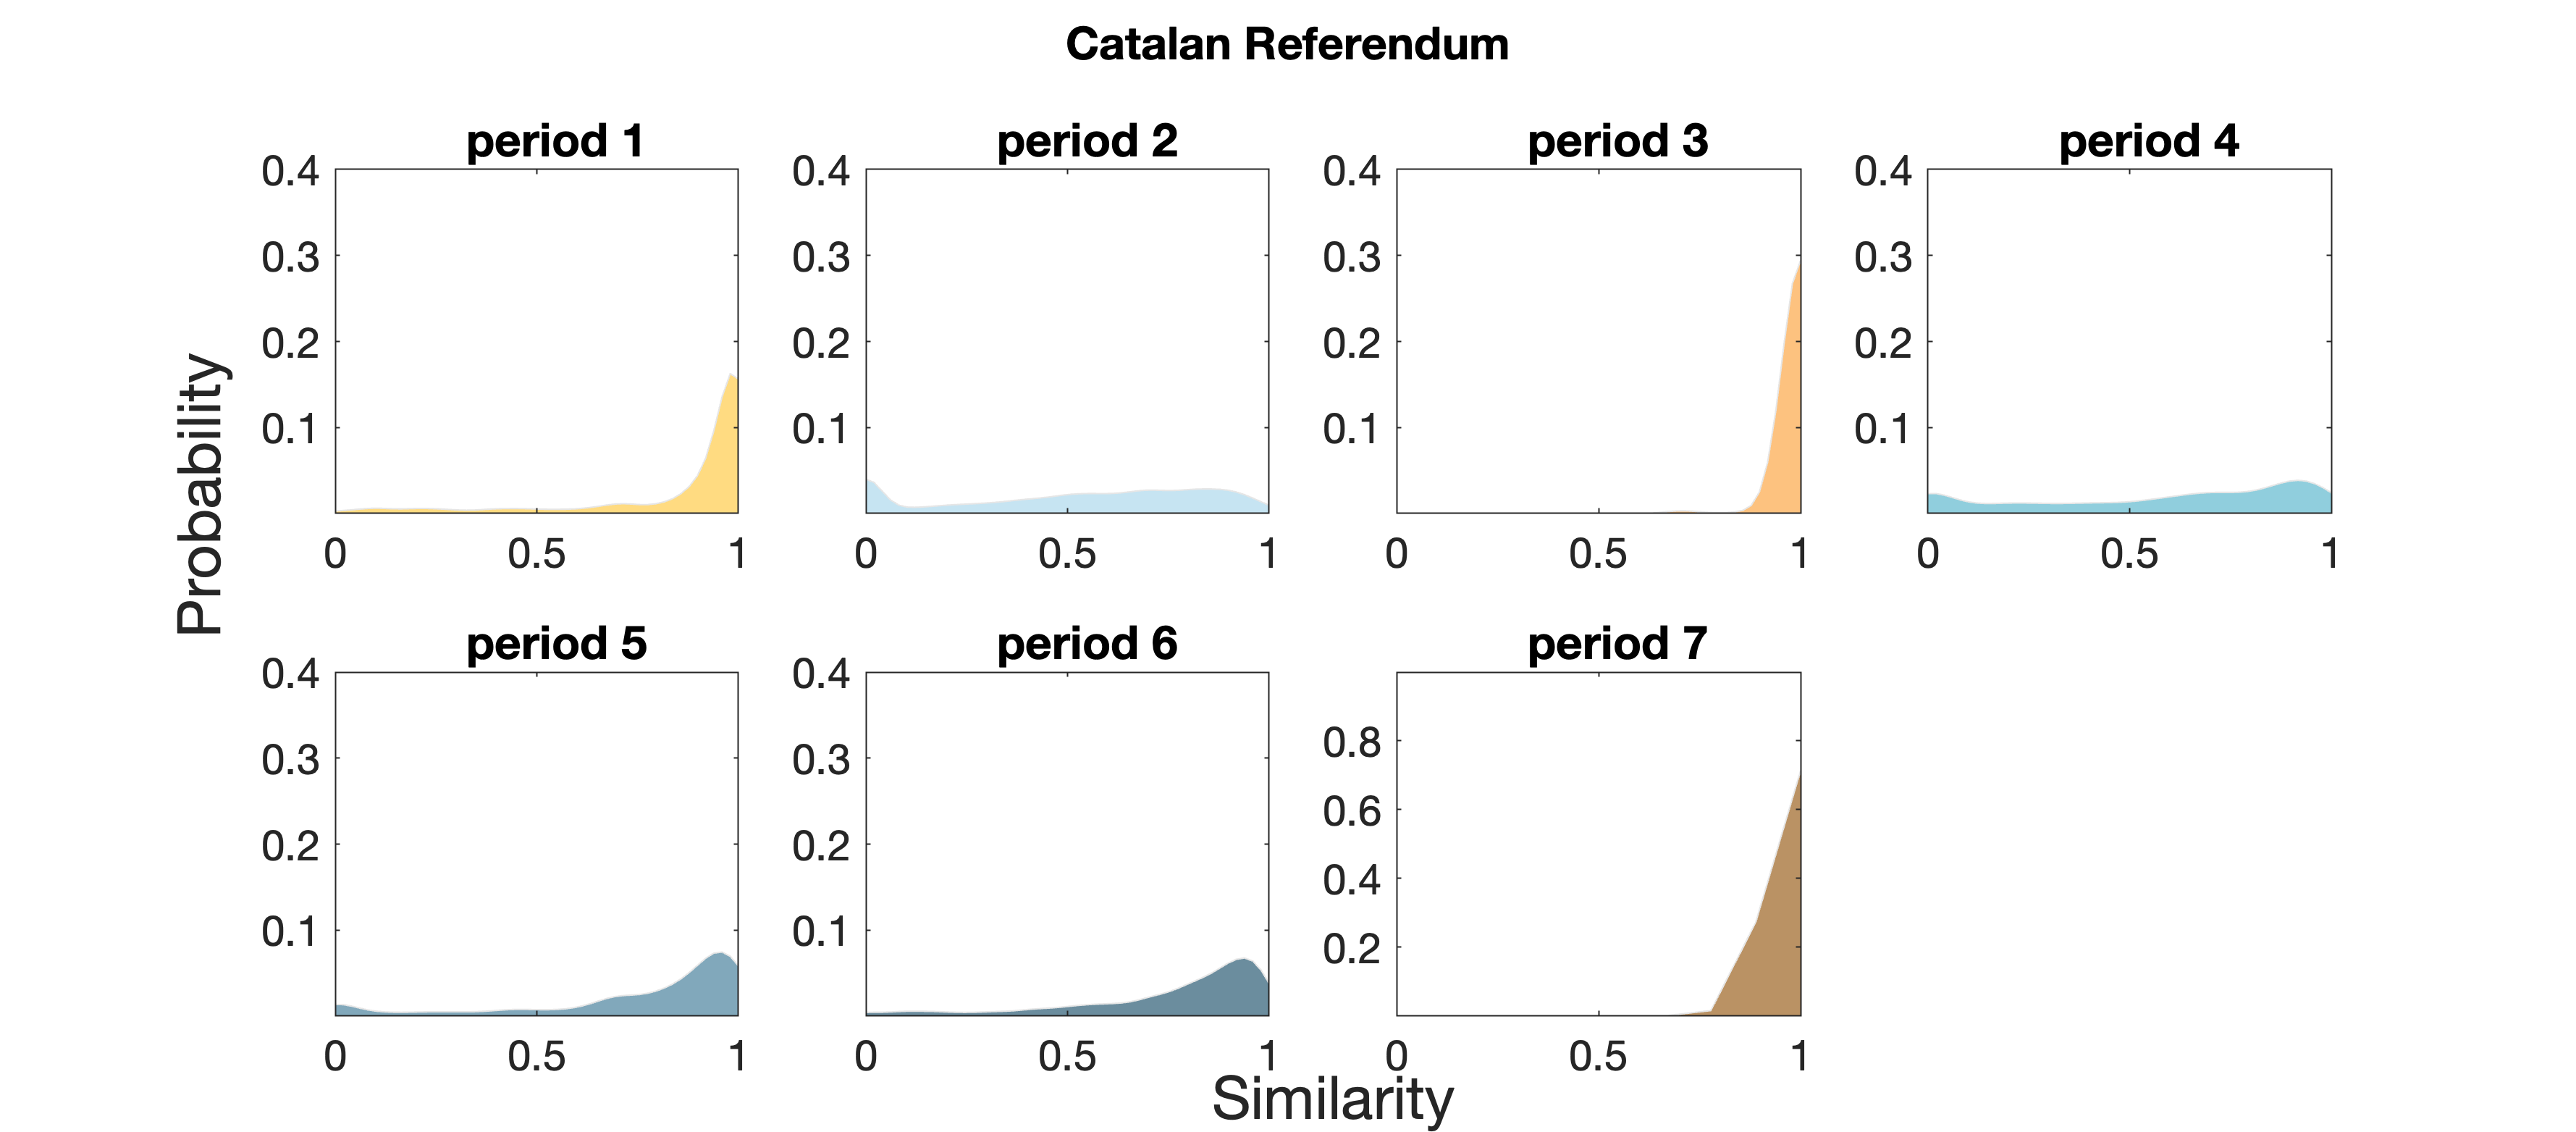
\includegraphics[width=1.05\textwidth]{figures/chp3/similarity_catalonia_nolog.png}
   
    \caption[Cosine similarity distribution of user-topic vectors]{Cosine similarity distribution of user-topic vectors for the most active users of the Catalan referendum dataset. The cosine similarity has been calculated following Eq.~\ref{eqsim}. The most active users are the ones that have taken part in the discussion for at least $90\%$ of the time and posted a minimum of $10$ tweets within the whole period, which comprise around $400$ accounts. Shaded areas denote peak periods.}
   \label{chp3:fig:6}
\end{figure}

These last two results --the heterogeneous distribution of activity during peak events shown in Figure~\ref{chp3:fig:4b}, and the consistent number of topics over the periods,  as detailed in Table~\ref{tab:nets}--, define a precise scenario. During periods of ordinary activity, users focus on their own interests, and hashtags compete for attention inside the specific discussions. When collective attention is captured by an external event, initial topics stay active but generate less activity. To visualize how attention shifts from the different topics over time, we have created an alluvial diagram for the activity around the topics through periods. Figure~\ref{chp3:fig:5} shows the diagram for the Catalan referendum dataset (we have obtained equivalent results for the other datasets, not shown). The size of each block is proportional to the number of tweets, and only the flows of activity of the four bulkiest topics are considered. During peak periods (first, third, and seventh), the flows merge into one single topic (``Diada'', ``9N2014'' and ``9N'', respectively). When external events dissipate, flows break apart into different discussions again, and some hashtags are not posted during calm intervals, but recover popularity during high-activity periods. This behavior can see seen, for example, by looking at the extensive flows moving right from the first period to the third one.


\subsection{Users' similarity}
\label{chp3:2.2}

Having previously investigated how extraordinary events influence hashtags' use and activity, we can now concentrate on the opposite side of the equation: user behavior. We measure the overlap in interests between user pairs with the cosine similarity of user-topic vectors. A higher average similarity will indicate that people are paying more attention to a smaller number of topics, which will lead to more competition. \\

Figure~\ref{chp3:fig:6} shows the distribution of similarity between all potential pairs of the $400$ most active users from the Catalan referendum dataset (active users for at least $90\%$ of the time and posting at least $10$ tweets containing hashtags).  The outcomes  match what we discovered for the hashtags, as expected. Users' similarity is homogeneously distributed between $0$ and $1$ during periods of low activity (i.e., second and fourth periods), indicating that independent discussions with nearly equivalent activity are occurring. On the other hand, high activity periods are marked by a nearly perfect alignment of users, with the similarity distribution peaking at exactly one: everyone is chatting about the same issue.

\begin{figure}[t]
    \centering
   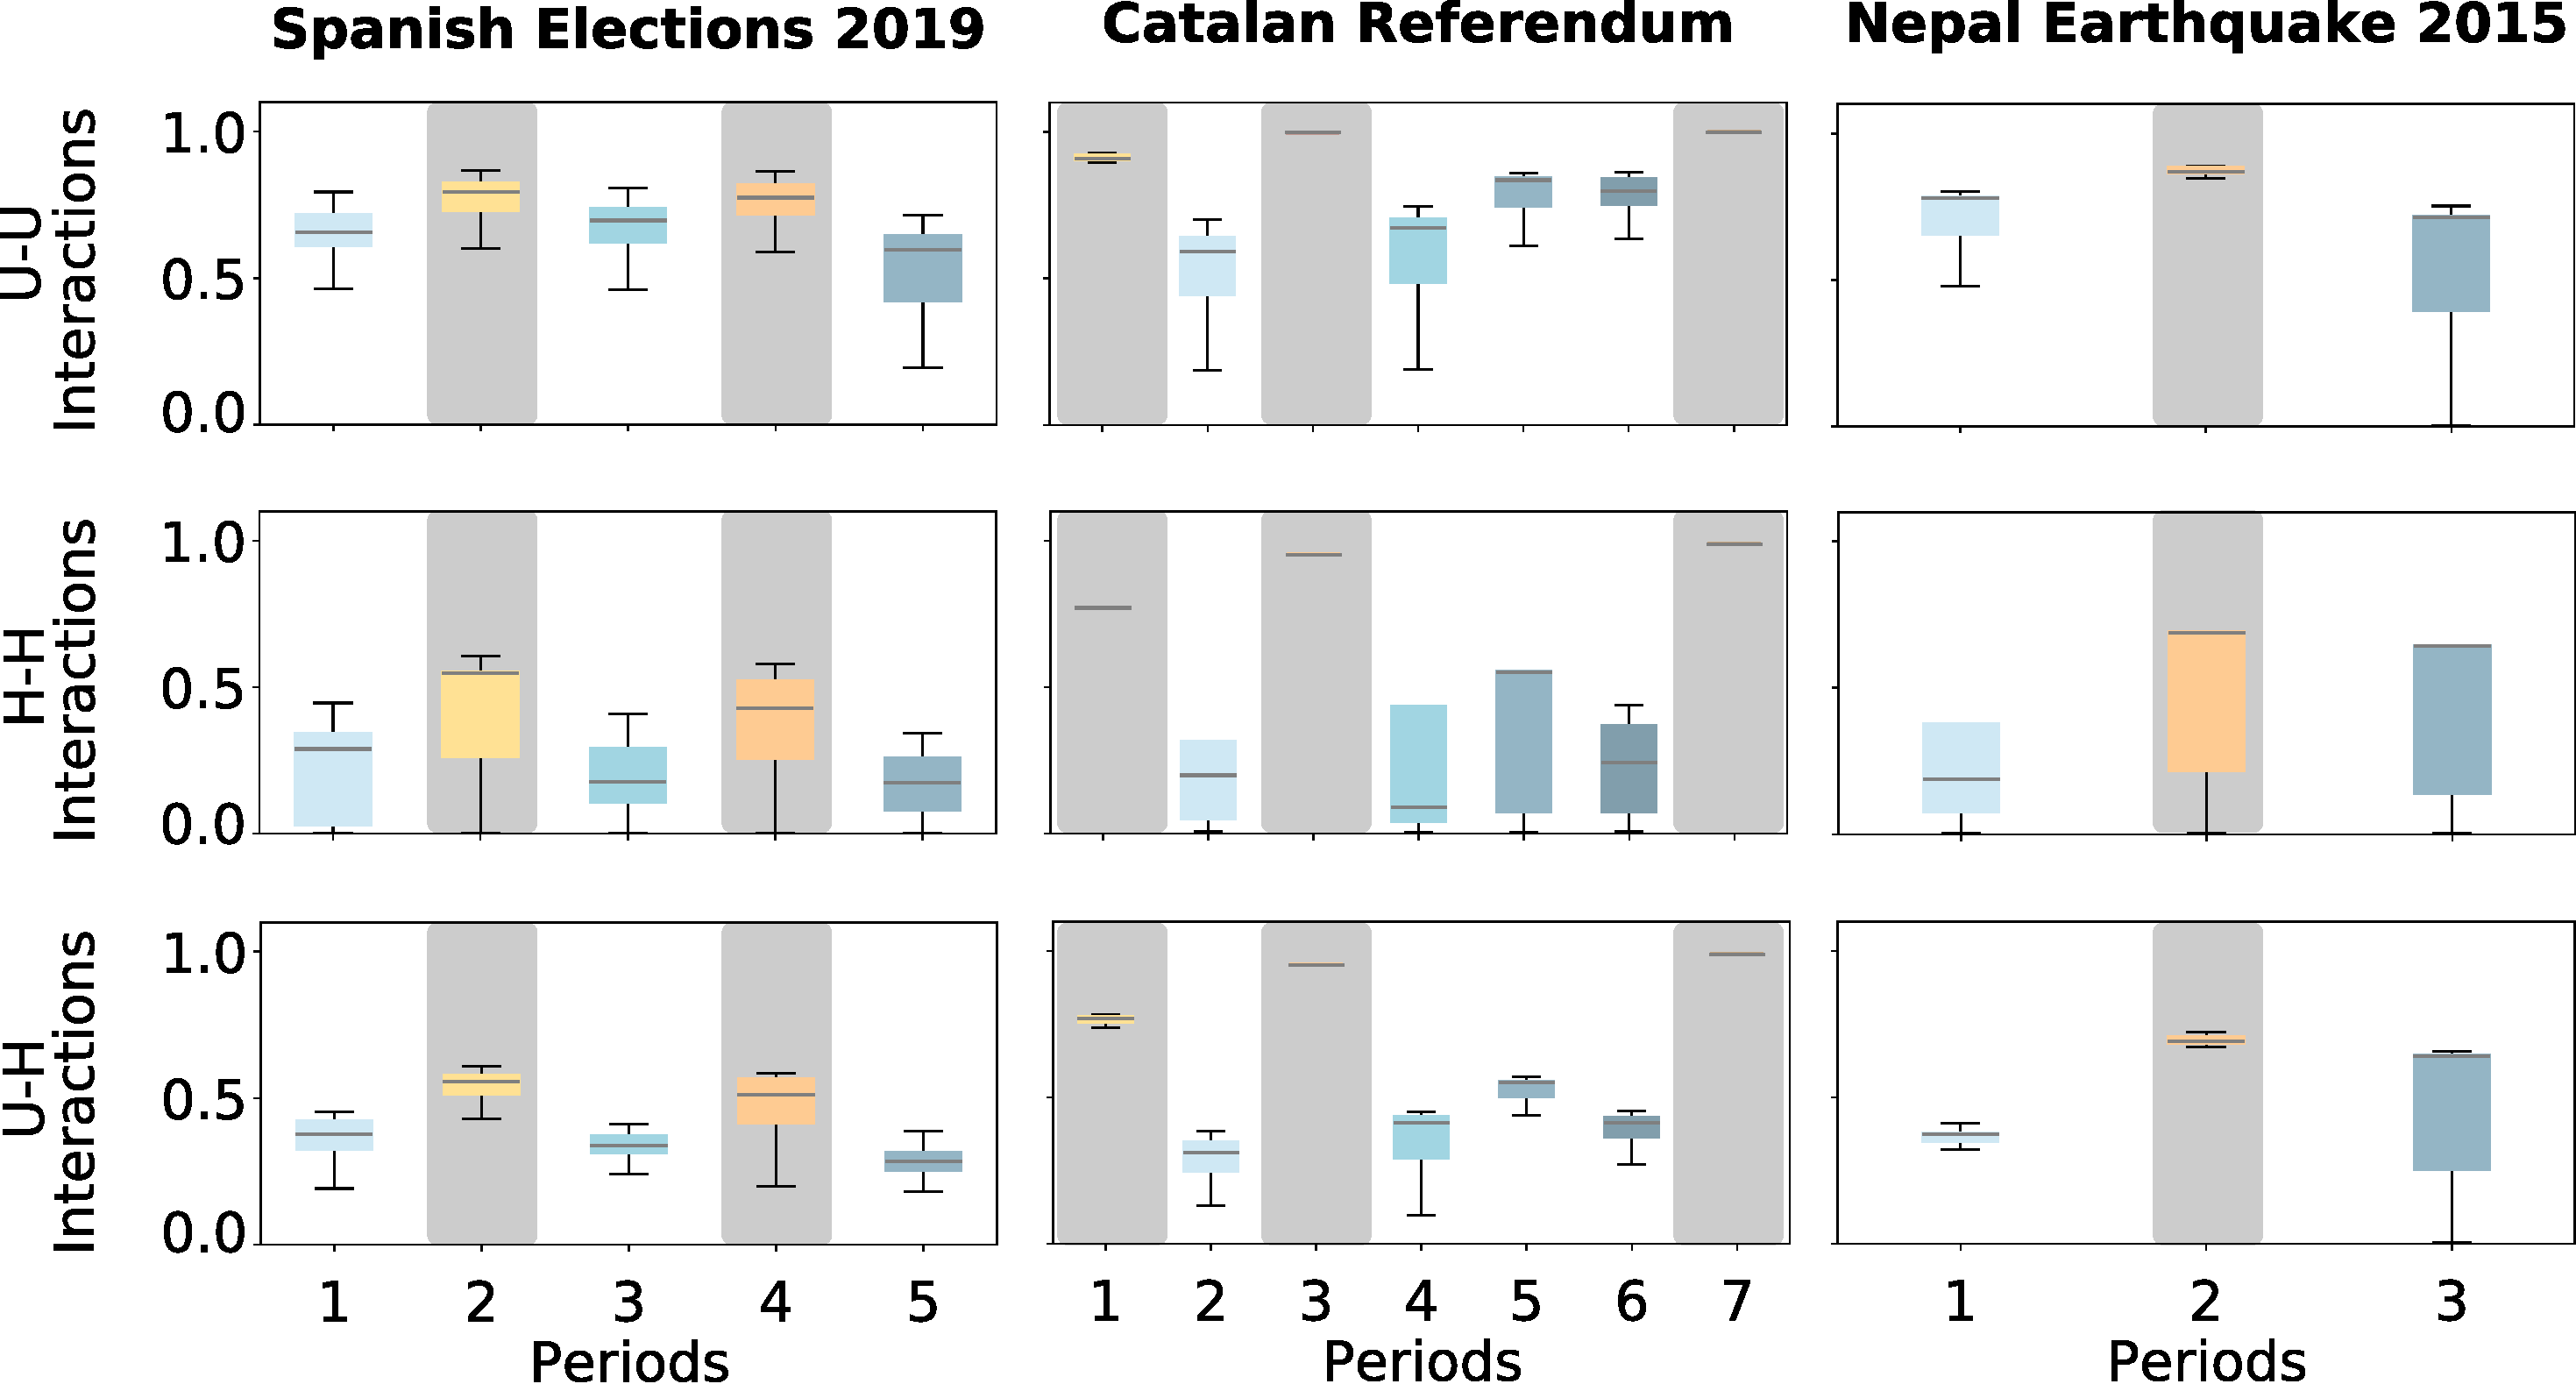
\includegraphics[width=1\textwidth]{figures/chp3/fig7.pdf}
   
    \caption[Strength estimations for competitive and mutualistic interactions]{Strength estimations for hashtag-hashtag and user-user competitive interactions (first and second row), and user-hashtag mutualism (third row) for the $400$ most active users and the hashtags they wrote. The interaction strength is the average value of the elements of the matrices $\beta^{HH}$, $\beta^{UU}$, and $\gamma^{UH}$. The gray horizontal line in the box plots is the median of the distribution, and the colored boxes have a length corresponding to the 25th-75th percentiles. As usual, shaded areas mark peak periods.}
   \label{chp3:fig:7}
\end{figure}



\subsection{Quantifying competition and mutualism during exceptional events}
\label{chp3:2.3}


\begin{figure}
    \centering
   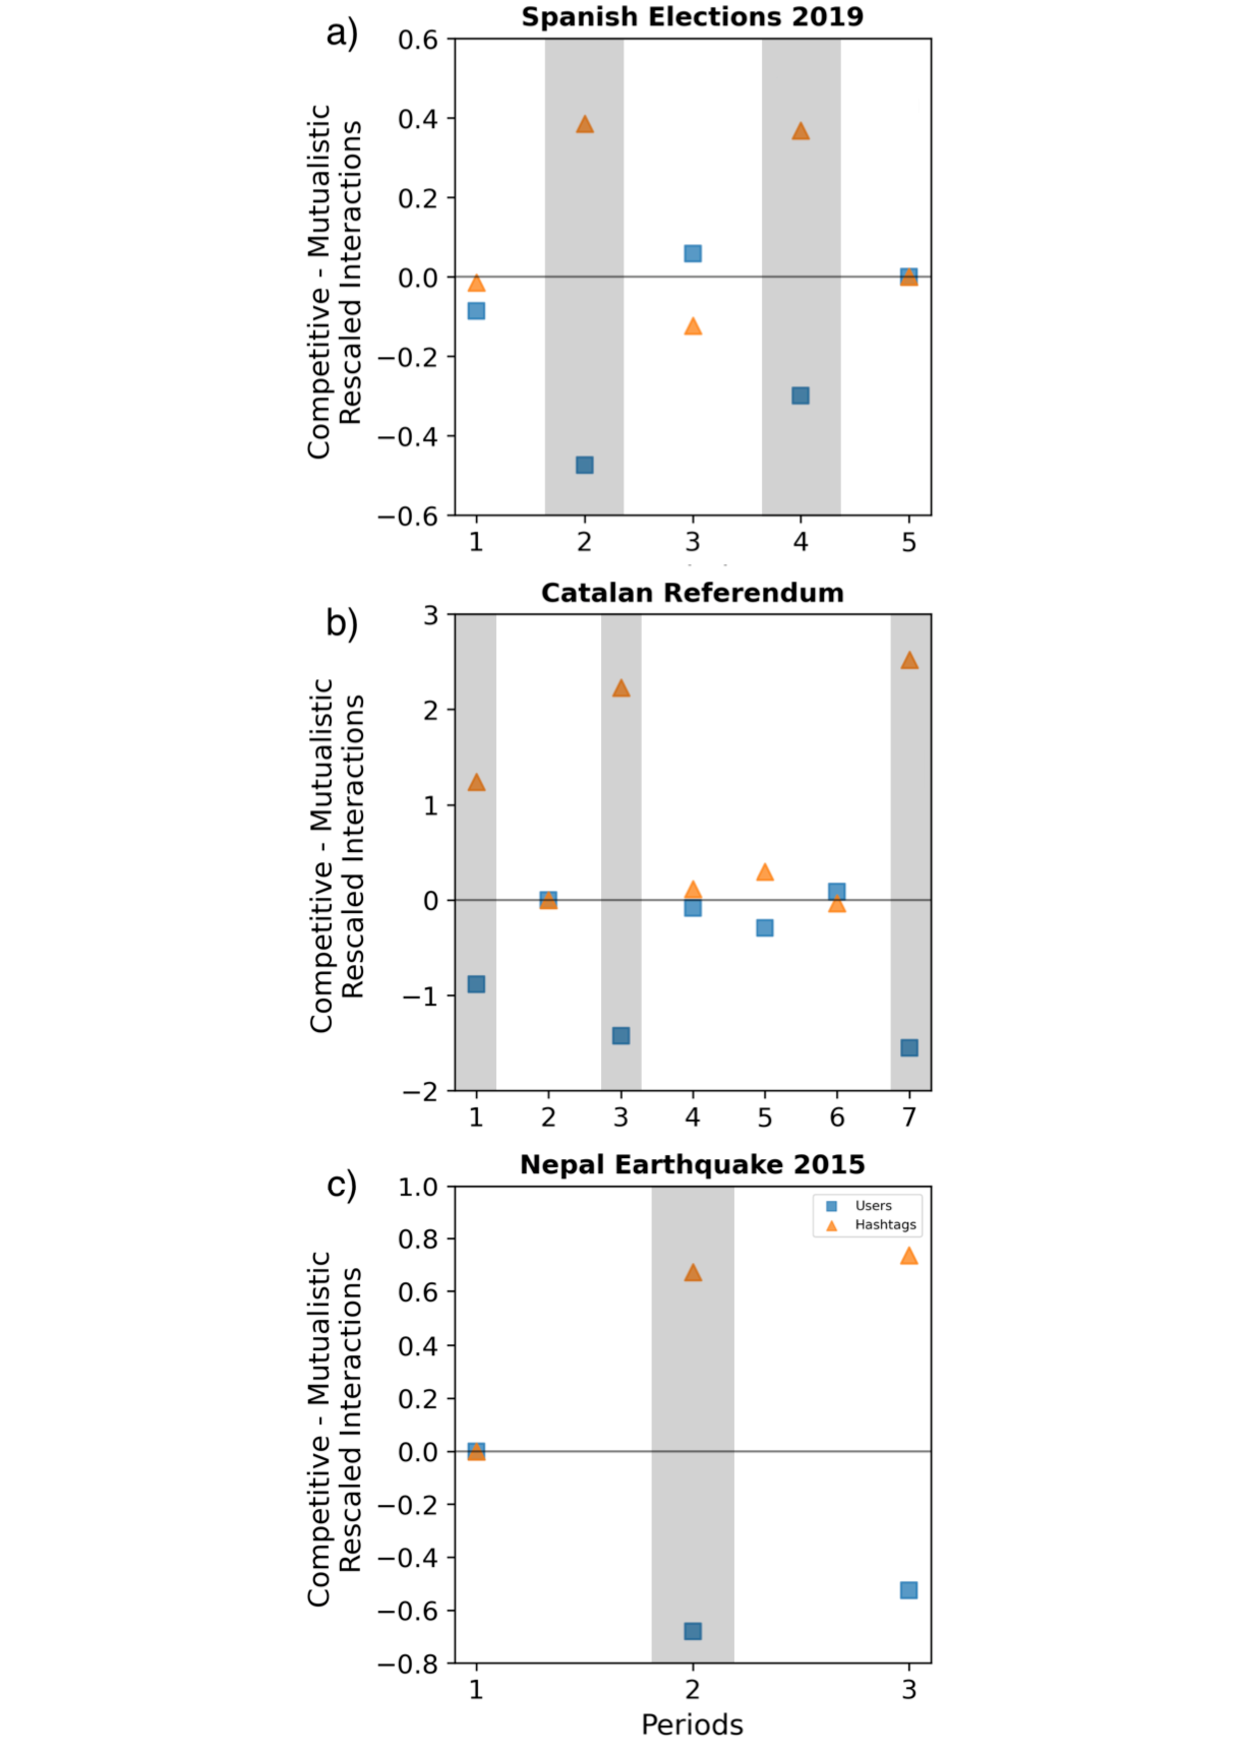
\includegraphics[width=0.5\textwidth]{figures/chp3/fig8.pdf}
   
    \caption[Rescaled difference between competition and mutualism]{Rescaled difference between competition and mutualism over all the periods.  Each point is the average difference between competitive and mutualistic strength for each user (or hashtag). The difference has been rescaled with the values observed during the calmest period (fifth period for the Spanish elections, second period for the Catalan Referendum dataset, and first for the Nepal earthquake). Shaded areas indicate peak periods.}
   \label{chp3:fig:8}
\end{figure}


The results so far in Figures~\ref{chp3:fig:4a} to~\ref{chp3:fig:6} can be easily understood in terms of visibility maximization. In normal times, users tend to focus on their specific interests and aim for visibility inside their communities. Important events can captivate everyone's attention, leading users to join the conversation. This simple response, driven by individuals' strive for visibility, has some complex consequences. On the one side, an increase in competition for attention. With a huge amount of messages covering one single topic, the probability for each user's ideas to be heard decreases. On the other side, the use of hashtags related to relevant topics can lead to a mutualistic (positive) interaction as they allow us to reach a larger audience. Our goal is to quantify the strength of both these interactions to understand which one dominates the dynamics in the different periods.  \\

To achieve this, as explained in Section~\ref{chp3:1.4}, we construct three interaction networks from user and hashtag similarities --two for competition ($\boldsymbol{\beta^{UU}}$ and $\boldsymbol{\beta^{HH}}$), and one for user-hashtag mutualism ($\boldsymbol{\gamma^{UH}}$)-- and examine changes in node strength over time. The benefit of estimating competitive and mutualistic strengths using niche overlap  \cite{cai2021niches} is that it rescales both terms, making them comparable. By doing so, we may calculate how much each factor contributes to the dynamics of the system. \\ \\

\begin{figure}
    \centering
   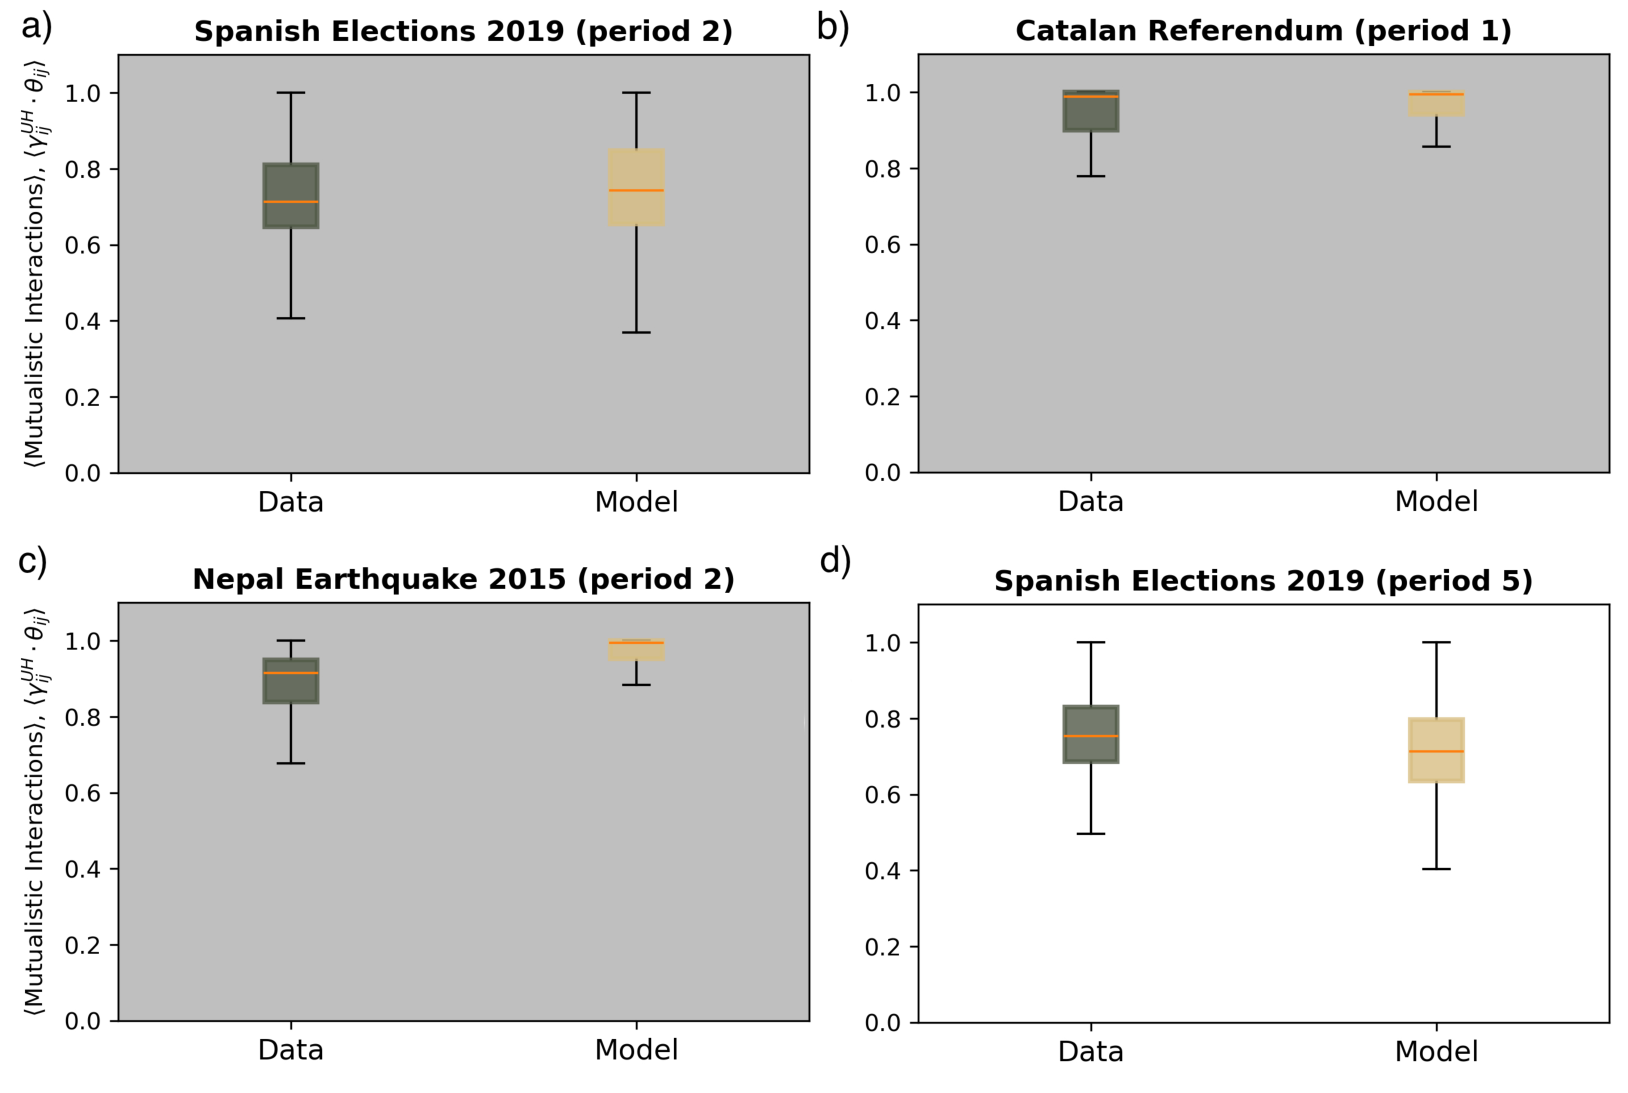
\includegraphics[width=1.05\textwidth]{figures/chp3/fig9.pdf}
   
    \caption[Effective interactions recovered from the visibility optimization model]{The effective mutualistic interaction strengths $\gamma^{UH}_{ik}\theta_{ik}$ extracted from the data (dark brown boxes) to compare with the values obtained with the visibility optimization model (light brown boxes). (Panels a-c) For the calm-to-peak transitions, the model's initial conditions are as follows: 
To emulate an exceptional event, the initial values of matrices $\beta$ and $\gamma$  are the empirical matrices of a high activity period, which correspond to the $400$ most active users together with the hashtags they used from a. In particular, we choose period $1$ for the Catalan referendum and period $2$ for the Spanish elections and the Nepal earthquake. Moreover, the user-hashtag interaction matrix $\theta$, which indicates whether a user posted a specific hashtag, is extracted from the previous or next calmer period. These periods are $1$ for the Spanish elections and the Nepal earthquake, and period $2$  for the Catalan referendum). (Panels d) For the Spanish elections peak-to-calm transition, matrices $\beta$ and $\gamma$  are now selected from a calm period  (period $5$), while matrix $\theta$ is taken from the previous high-activity period (period $4$).  In all the transitions, the model runs for $5 \times 10^4$ rewiring attempts. The rest of the parameters are $\Omega_c = \Omega_m = 0.08$ for Spanish elections and Nepal earthquake datasets, and $\Omega_c = \Omega_m = 0.1$ for the Catalan referendum. The box plots represent the distribution of the values $\gamma^{UH}_{ik}\theta_{ik}$. The orange lines are the median of these distributions, and colored areas delimit the 25th and 75th percentiles.}
   \label{chp3:fig:9}
\end{figure}

Box plots of the interaction strength distributions for the three datasets are displayed in Figure~\ref{chp3:fig:7}. During high-activity periods, we consistently observe an increase in both competition and mutualism. The evolution of the two interactions does, however, differ from one another. Even in times of low activity, users still face competition. Its strength is only marginally increased when an external event occurs and attention shifts as a result. Instead, hashtag competition generally declines during calm periods and increases significantly during events. Similar results are observed for mutualistic interactions, with moderate values (with a median of approximately $0.4$) for resting periods and dramatic jumps up to nearly $1.0$ during peaks. \\

Given the previous results, however, the fundamental question of which mechanism weighs most for users and hashtags remains. To provide an answer, in Figure~\ref{chp3:fig:8}, we show the average difference between competitive and mutualistic strength for each of the $400$ users and related hashtags, rescaled now to the value they had during the calmest period of their corresponding dataset. We notice two distinct behaviors for users and hashtags. As mutualistic strength grows more than competitive strength at peak intervals, the effective competition experienced by users reduces significantly.  Users are encouraged to actively participate in the main debate by this effect since they can see that their posts are getting greater attention. 
Instead, there is typically more hashtag competition during events than there is during other periods. This is likely because hashtags unrelated to significant event topics will receive very little attention, whilst those linked to key topics must withstand the additional pressure brought on by user interests. \\ \\

\subsection{Modeling attention switches during exceptional events}
\label{chp3:2.4}

After evaluating the effective competition that the users faced, we try to identify the key factors that led to the reorganization of the information topics that we observed in the datasets. We use the visibility optimization model described in Section~\ref{chp3:1.3} and \cite{palazzi2021ecological} to do that. While the authors in \cite{palazzi2021ecological} use synthetic data to simulate the model to replicate the structural reorganization of the user-hashtag interaction networks during external events, here we take a step further and use the matrices that have been directly created from the data to inform the model. This will allow us to test the idea that the major cause of the concentration of public attention is visibility optimization and its resulting decrease in perceived competition. \\

In order to demonstrate that visibility optimization is the main driver of the dynamics, we run the model during a transition of two successive periods of our data: a calm period followed by an event --for instance, periods $1$ and $2$ in the dataset for the Spanish elections-- and then, we compare the user-hashtag network optimized at the end of the simulation ($\gamma_{ik}^{UH} \theta_{ik}$) with the one derived from the data.
 (model's parameters are listed in the caption of Figure~\ref{chp3:fig:9}). After that, we confront the optimized effective mutualistic interactions $\gamma^{UH}_{ik}\theta_{ik}$ with the one obtained from the peak period data using the hashtag co-occurrence networks and cosine similarity. Additionally, we examine whether visibility optimization can also explain the transition when users' attention shifts back to their primary areas of interest after the peak has vanished. To do that, we begin the model using matrices $\boldsymbol{\beta^{UU}}$,  $\boldsymbol{\beta^{HH}}$ and $\boldsymbol{\gamma^{UH}}$ from a resting period, and let optimize the matrix $\boldsymbol{\theta}$ from the preceding peak period. \\

In the box plots of Figure~\ref{chp3:fig:9} we compare the matrices from the data and the model for the peak-to-calm transition for the Spanish elections (Figure~\ref{chp3:fig:9}d) and the calm-to-peak transitions for all three datasets (Panels a to c). The fact that there is a consistent agreement between the matrices $\gamma_{ik}^{UH} \theta_{ik}$ in each example means that the optimization method alone can accurately duplicate the intensity of the user-hashtag interaction networks that were derived from the data. This supports our earlier findings, which showed that users who pay attention to hot subjects during external events face less intense competition, and that visibility optimization encourages users to return to their original interests once the event has ended.

\section{The science of hype: discussion}
\label{chp3:3}

The emergence of OSNs (Online Social Networks) altered how our society processes information. We switched from the traditional one-emitter many-receivers model that characterized mass media to a complex network where everyone serves as both a producer and a consumer simultaneously. To prevent information processing distortions like the propagation of false news or the emergence of echo chambers that might skew the democratic discussion, it is crucial to understand the forces that determine our collective behavior in this new environment.\\

In this Chapter, to measure the competition for attention that OSN users face during unusual events and how they react to it, we drew on the similarity between natural and information ecosystems. Specifically, we were able to measure the strength of competitive and mutualistic interactions between users and hashtags using a modeling approach based on ecological niche theory. Our findings demonstrate that, while competition between users and hashtags grows significantly during the event's climax, it is also strongly correlated with a rise in users' mutualism. Interestingly, this turns into a positive gain in terms of interactions for users --who, on average, already face greater levels of competition-- thereby decreasing the net competitiveness. On the other hand, this effect is modest for hashtags, that ultimately experience greater competition. Furthermore, the patterns seem universal since they are independent of the type of event (social, political, or natural) as well as the data-collecting method.\\

Our results shed light on the mechanisms behind the emergence of collective attention in online social media, which has critical consequences for group behavior and information processing. The authors of \cite{palazzi2021ecological} show that external events result in a structural shift in the user-hashtag interaction network by using the same visibility optimization model. Here, by informing the same model with actual data, we are able to explain why this new arrangement is better for users. The fact that the numerical simulations agree with the data indicates that users behave as they do because they want to be seen. Users who participate in online debates tend to increase their visibility within the themes that interest them, creating intense competition inside each topic. The same visibility maximization encourages agents to follow the dominant topic as an event approaches, raising competition but also expanding viewers. This rearrangement of interactions is stable, however, because mutualistic benefits outweigh the more intense competition. \\

Although it is exciting that our modeling has been able to provide insights into users' behavior, it still idealizes the complex dynamics that exist in online social systems. For instance, the assumption that the strengths are the same for competitive and mutualistic interactions $(\Omega_c = \Omega_m)$ is one more simplifying premise in our paradigm. Decreasing the parameter space's size, which is a frequent practice in ecological modeling, is necessary for our framework to properly compare the interaction matrices $\boldsymbol{\beta}$ and $\boldsymbol{\gamma}$. Nevertheless, extracting $\Omega$ from raw data would allow us to answer other questions that require a more accurate description of competitive dynamics in OSNs. \\

Finally, we implicitly presume that competitive (mutualistic) interactions only occur between species of the same (different) guilds, as in the majority of ecological models. However, this approach ignores some second-order processes, such as intra-guild mutualism, which has recently been studied in the literature on ecological modeling \cite{crowley2007,stanton2003}. These effects manifest as beneficial interactions between users or hashtags. For example in Twitter, the increase in exposure a user gets when their tweets are retweeted by another user, or how coexisting  hashtags in the same tweet enable each of them to reach a wider audience. These processes might be included to better understand the dynamics of endogenous Twitter events, the rise of important users, and other phenomena.\\





\chapter{Uncovering online tapestries: Ecological patterns in information ecosystems}\label{chp:4}

Many complex systems, such as ecosystems or social systems, can benefit from interdisciplinary approaches to be better understood and effectively managed. In particular, online communication systems are composed of many interconnected agents, and fully characterizing  them  requires developing innovative models that draw from insights from multiple fields. As a case in point, in Chapter~\ref{chp:3}, we proposed a driver for collective attention --the optimization of visibility-- and validate it using an ecology-inspired model. In this Chapter, we investigate the dynamics of online social networks at an alternative scale, which looks at the fingerprints of drivers and constraints in a more general way. They are not obvious a priori, and to infer such characteristics we look for quantitative invariants that are consistently repeated, patterns. Following the bridge we drew in this thesis between natural and information ecosystems, we assume that ecological and social complex systems, despite the differences in the nature of their microscopic description, may exhibit similar complex behavior in the form of patterns on the macroscopic scale. Identifying a pattern is the first step to discovering the  drivers of the dynamics, as every proposed process must be able to reproduce those patterns.\\
   
%%%%%%%%%%%%%%%%%%%%%%%%%%%%%%%%%%%%%%%%%%%%%%%%%%%%%%%%%%%%%%%%%%%%%%%%%%%%%%%%%%%%%%%%%%%%%%%%%%%%
\section{Why: the purpose of looking and finding patterns\label{chp:4:1}}

Here, we ask whether information ecosystems share the same general laws found in natural ecosystems. Given the analogies that can be drawn between the two systems and their success in creating new insight and applications \cite{borge2017emergence,palazzi2021ecological,plata2021neutral,calleja2021quantifying,tovo2021upscaling}, this research question is the logical step towards a fruitful cross-fertilization of the two worlds. If hashtags are seen as species, we can start keeping track of what we observe in online social systems to analyze what is happening with an ecological lens. By counting individuals in ecosystems, we have discovered several universal laws; such as that in any community of species, there are a few very abundant species and many rare species --the so-called Relative Species abundance distribution 
\cite{brown1995macroecology,preston1948commonness}. Does the social counterpart of this pattern exist? If so, would it have the same shape and features as the natural version? For example, would a potential abundance distribution of hashtags change with the size of the system as the species' abundances change with the scale of the community? \\

The possible existence of common patterns would suggest that there may be universal principles that drive the dynamics of natural ecosystems and online social networks (information ecosystems). Then, all the new questions that arise from this ecologically-inspired approach could take advantage of the theory once developed to explain the patterns in nature, for example, niche theory \cite{hutchinson1957concluding} and neutral dynamics \cite{hubbell2001unified} (that it was in turn borrowed from molecular genetics \cite{kimura1983neutral}). Another benefit of finding general patterns is that they have allowed for some simplification that has exceptional predictive power. In ecology, they are used to estimate the number of species that will become extinct as a result of habitat destruction, and how many species are present in ecosystems that are too large or difficult to sample extensively \cite{brown1995macroecology}. Recently, this extrapolation approach has been applied in human activity data to upscale the number of components in human communications (emails, words) as the size of the system increases \cite{tovo2021upscaling}. \\

In this context, we look for emerging patterns among a very heterogeneous group of datasets. They are reasonably not expected to share the same type of constraints, selection criteria, or optimization principles, given the radically different nature of their discussions and sampling methods \cite{zubiaga2018}. In turn, the selected patterns are widely known in ecology and revolve around complementary aspects of communities like their fluctuations in time and scale. 
%If these quantitative patterns are found in all our datasets, they may provide information about the commonalities of information ecosystems. 
 We then take a step further and investigate some aspects of the possible origin of the patterns, resampling our datasets according to a null model to answer how much of the observed patterns may be due to chance. In particular, we use a multinomial sampling model that only takes the frequencies of the hashtags into account. It lacks the details and constraints of the environment in which the hashtags have been generated, making it a useful null model that has been tested in the study of microbial communities \cite{grilli2020macroecological} or component systems like Lego sets \cite{lego}.
 
%- In many, but not all, of these models a preferential attachment principle is at the origin of the emergence of the power-law distribution of component frequencies. (nosotros tenemos algo así en el paper de maría  y el quantitative para explicar los cambios en estructura e intensidad de interacciones durante eventos)
%%%%%%%%%%%%%%%%%%%%%%%%%%%%%%%%%%%%%%%%%%%%%%%%%%%%%%%%%%%%%%%%%%%%%%%%%%%%%%%%%%%%%%%%%%%%%%%%%%%%%

\section{Where: the data  for finding macropaterns\label{chp:4:4}} %Describe data preparation, set some vocabulary and notation

%Explain datasets and their collection (briefly), set some vocabulary
 To test whether  patterns exist in information ecosystems, it is important to search for them in different contexts. If a pattern only appears in one dataset, maybe it emerges because of a particularity of that dataset. Since we are interested in quantitative invariants, common to online social networks in general, our data collection has to be as representative as possible. For this reason, we look for patterns across a very heterogeneous collection of $11$ datasets from the microblogging platform Twitter. The datasets are related to an event, whose nature varies: politics, sports, breaking news, etc.  We can divide them according to whether the event was planned (like elections or sporting contests) or was unexpected (like scandals or natural disasters). Another dataset is a random sampling from the $1\%$ of all tweets geolocalized in the UK. It serves to check whether some patterns' features are characteristic of datasets that revolve around events or are instead common to the whole communication process. The main characteristics of the datasets that concern us are presented in Table~\ref{chp:4:tab}, where we can observe large differences in their duration and size in terms of the number of posts (or tweets) harvested. The evolution of the number of times hashtags are posted can be observed in Figure~\ref{fig:4:totabun}. \\


\begin{table}[t]
\centering
\caption[Main features of the datasets]{Main features of the datasets involved in the study, sorted by the total number of \textit{different} hashtags. The ``Type'' column indicates whether the event was expected (E), unexpected (U) or it was not an event at all but a random sampling (R).}
\label{chp:4:tab}
\begin{tabular}{lcccc}
\hline
\textbf{Dataset}     & \textbf{Type}        & \textbf{Posts} & \textbf{Hashtags} & \textbf{Days} \\ \hline \hline
Mexican Elections  & E   & 191788     & 158                 & 1             \\ \hline
Scottish Referendum  & E & 429901     & 313                 & 23            \\ \hline
Catalan Referendum  & E  & 222783     & 375                 & 69            \\ \hline
St. Patrick's Day  & E  & 2882010    & 1591                & 3             \\ \hline
Brexit           & E     & 182629     & 1689                & 69            \\ \hline
UK random Sample  & R    & 1649482    & 1833                & 9             \\ \hline
Ferguson Unrest    & U   & 8782071    & 2811                & 17            \\ \hline
Spanish Elections  & E   & 4882546    & 2952                & 15            \\ \hline
Panama Papers     & U    & 5044378    & 3696                & 23            \\ \hline
Euro 2012      & E       & 8992157    & 4361                & 34            \\ \hline
Nepal Earthquake  & U    & 12004187   & 5032                & 23            \\ \hline
Hurricane Sandy   & U   & 5658525    & 5353                & 6            \\ \hline
\end{tabular}
\end{table}

\begin{figure}[t]
     \centering
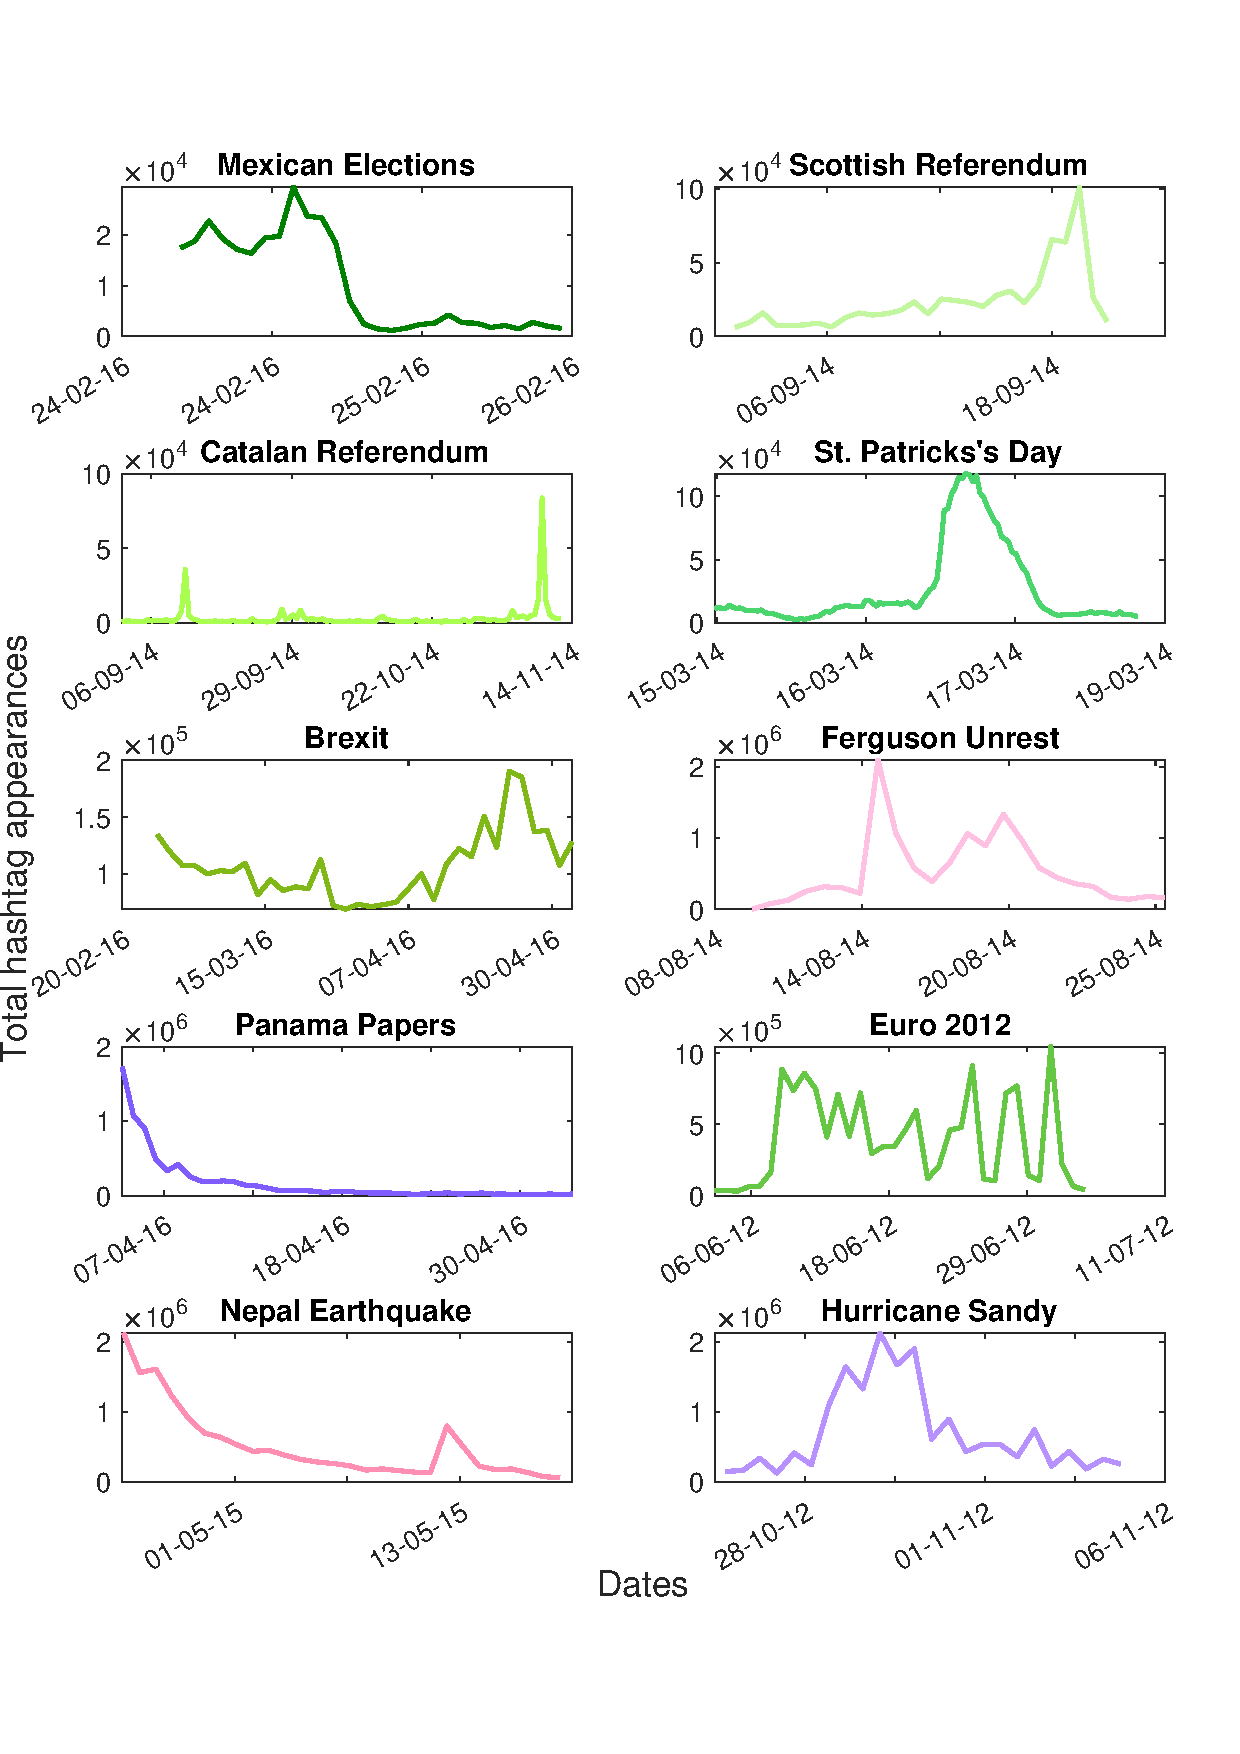
\includegraphics[width=\columnwidth]{figures/chp4/total_abuncances_vertical.pdf}
 \caption[Total hashtag abundances]{ Total hashtag appearances where the events of each dataset can be observed as peaks. }
\label{fig:4:totabun}
\end{figure}

Moreover, ecological patterns are usually defined within a community or are comparisons across communities.  These ecological communities are not straightforward to define, as dispersion and environmental factors can dilute their boundaries. Here, in order to represent communities, we have divided our datasets into a collection of posts referred to as bins. Our communities are then represented as different bins with constant sampling effort, that is, the number of posts where the hashtags can be found is fixed. Having a constant sampling effort prevents biases in the patterns. It is the equivalent of counting species in regular patches of land to characterize the community. The sampling effort, in our case, is represented as a certain number (or volume) of posts. A \textit{volume} bin consists of $V$ consecutive posts (Figure~\ref{fig:image}). We have selected a $V$ for each dataset according to its size and checked that our results remain almost unaffected by creating bins with different reasonable values of $V$. \\



%A bin is a population sample, i.e. a collection of posts that represent a community. \\

%Bins are generated in two ways depending on the nature of the patterns to detect.  If we are dealing with temporal patterns, we group the tweets according to their posting time (left-hand side of Figure~\ref{fig:image}). A bin then consists of the posts that have appeared during a fixed time interval of length $T$.  These time intervals are constant and consecutive, and each bin is thus refereed as a \textit{temporal} bin. Furthermore, we need a proxy when the patterns are not temporal but originally deal with abundances or species within a certain region or across different areas. For these patterns, space parallels with the sampling effort made to uncover the species. The sampling effort, in our case, is represented as a fixed number (or volume) of posts. A \textit{volume} bin consists of $V$ consecutive posts (right-hand side of Figure~\ref{fig:image}). 
%The bins are randomly sampled with replacement $B$ times, a technique known as bootstrapping. It is used to obtain better statistics of the dataset without assuming any underlying mechanism for the creation of the data. Bootstrapping is especially useful with small datasets, as a means to compensate for the distortions brought on by bursts of activity, which might not be entirely representative of the dataset. 
%Finally, we have checked that our results remain almost unaffected by creating abundance matrices with different reasonable values of $T$, and $V$.\\

Thus, a natural way to describe our datasets is employing a $H \times B$ abundance matrix,  where $H$ is the number of different hashtags in the dataset and $B$ is the total number of bins in which it has been divided. Each entry $n_{hb}$ represents the abundance, the number of posts of bin $b$ in which hashtag $h$ has appeared. Some key variables can be easily derived using the matrix representation. First, the total abundance of a bin $b$ is the column-sum $N_b = \sum_{h = 1}^H n_{hb}$. Notice that the number of hashtags in every volume bin is not constant. For each post, the number of hashtags may vary. The relative abundance of a hashtag is defined as  $x_{hb} = n_{hb}/N_b$, and it is normalized in such a way that $\sum_{h = 1}^H x_{hb} = 1$. Two other crucial observables are the mean relative abundance of a hashtag across all the bins $\bar{x}_h = \frac{1}{B} \sum_{b=1}^B x_{hb}$ and the total number of posts in the dataset $N = \sum_{b=1}^B N_{b} $.\\

To finish the data preparation, it is worth noticing a key difference between ecological and information ecosystems' data. Taking a simplified vision, in ecological experiments, there is usually not sufficient time, economic resources, and personnel to do a complete sampling. These problems usually result in subsampling and the impossibility to replicate experiments in different localities or habitats. For online social networks, the problem is on the other side of the spectrum. Data is abundant, albeit usually upon payment. We are said to be in the Big Data era for a reason. This means that even with pertinent data collection, we may end up with lots of spurious hashtags. For that reason, it is convenient to establish a method to discard those hashtags. As our datasets revolve around one or more events, and to reduce any noise that might have been caused by bots or misspelled hashtags, any hashtag that had been tweeted fewer than $75$ times was filtered out. We have verified that our results remain mostly unaltered when subjected to various filters.

%threshold for the number of bins in which a hashtag needs to appear to be considered in the analysis of patterns that are not sensitive to undersampling. When a hashtag appears at least in $50\%$ of the bins, we assume it is not spurious and has been involved in some discussion around the events. 

\begin{figure}[t]
     \centering
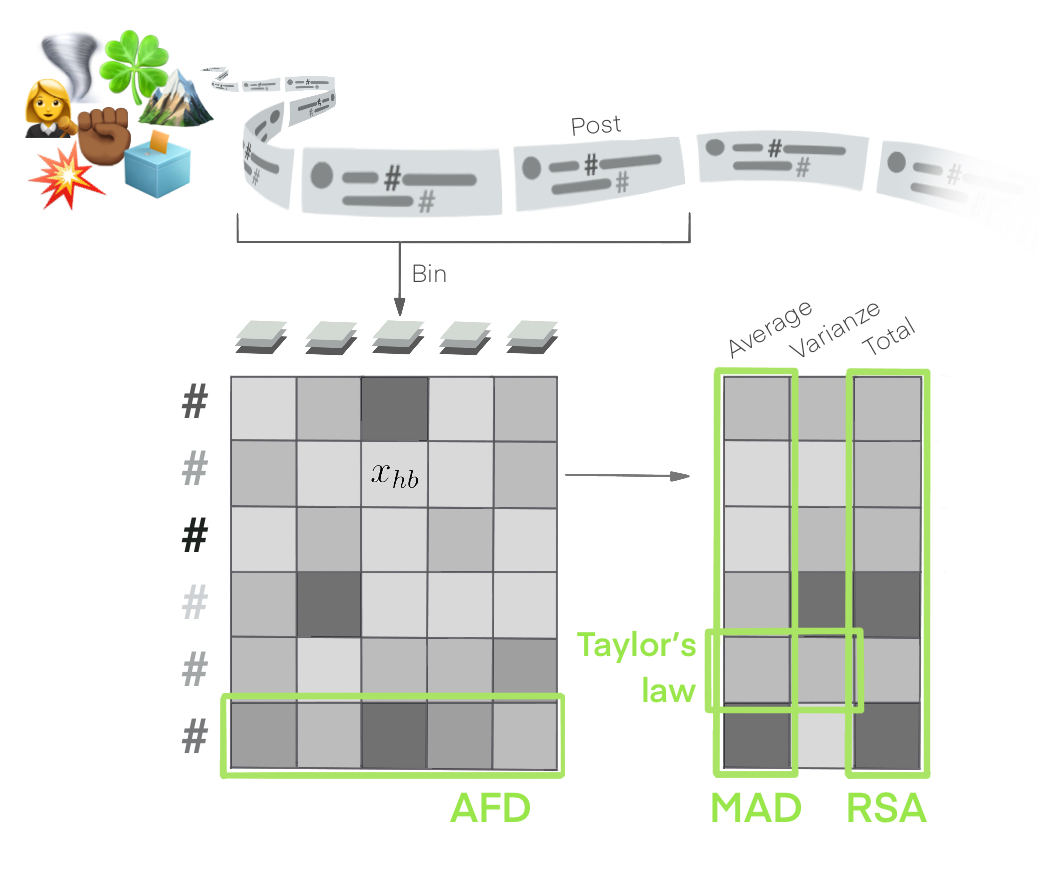
\includegraphics[width=\columnwidth]{figures/chp4/alagrilli.pdf}
 \caption[Data representation]{ The abundance matrix describes our datasets from the stream of posts of each event. After dividing the posts into bins, we aggregate the compositional data according to the pattern to uncover.}
\label{fig:image}
\end{figure}

%%%%%%%%%%%%%%%%%%%%%%%%%%%%%%%%%%%%%%%%%%%%%%%%%%%%%%%%%%%%%%%%%%%%%%%%%%%%%%%%%%%%%%%%%%%%%%%%%%%%%

\section{How: patterns for information ecosystems} %Define patterns, fitting, and particular data preparation methods if any
As we said, a large number of universal laws have been discovered in ecology. We have selected $6$ of them whose functional forms have been extensively discussed and have an ecological meaning that is transferable to information ecosystems, together with their applications in modeling and prediction. The patterns are the following: the abundance fluctuation distribution (AFD), Taylor's law, the mean abundance distribution (MAD), the relative species abundance distribution (RSA), the species-accumulation curve (SAC), and the short-term abundance change distribution (STAC). In the next paragraphs, the definition of these patterns is presented with a brief description of their importance. For a deeper review of the ecological implications of their forms, see Appendix~\ref{appen:patterns}.\\

%The regularities we have tested are defined for transversal data (see Figure~\ref{fig:image}), with the exception of the short-term abundance changes for longitudinal (temporal) data.

\paragraph{AFD:} The purpose of this pattern is to characterize the distribution of population abundance seen in different communities. To be more precise,  we refer to how the abundance levels of a single species change when it is measured in the different communities where it occurs. Ecologists have commonly  believed that population abundance is lognormally distributed \cite{May1975PatternsOS}, inspired by the fact that population growth is a multiplicative (rather than additive) process \cite{marquet2005scaling}. Moreover, a gamma distribution has also been postulated to describe the AFD and has obtained superior fits in some cases \cite{halley2002lognormality,grilli2020macroecological}. In the latter case, the probability species $h$ has a relative abundance $x$ in a bin is:
\begin{equation}
    \rho_h (x) = \frac{1}{\Gamma(\beta_h)} \left( \frac{\beta_h}{\overline{x}_h} \right)^{\beta_h}    \overline{x}^{\beta_h -1} \textrm{exp} \left( -\beta_h \frac{x}{\overline{x}_h} \right),
\end{equation}
where $\overline{x}_h$ is the mean (relative) abundance of species $h$, the parameter $\beta_h$ is its squared inverse coefficient of variation,  $\beta_h = (\overline{x}_h / \sigma_h)^2 $, and $\Gamma(\beta_h)$ is the gamma function.\\


\begin{comment}
Method:  
1) Choose the most abundant hashtag that is present in all bins 
	1.1) we just show one hashtag, and it is not the sampler (comprobar todo esto)
2)  Fit the relative abundance to gamma and lognormal (MLE maximum likelihood estimates). Why also checking lognormal? The gamma distribution is proposed, it is not derived.
3) Plot theoretical curve: Goodness of fit: chi2
4)  Log and Rescale the x-axis
\end{comment}


\paragraph{Taylor's law:} 
Empirical studies and models have observed that the variance in population abundance across communities $\sigma_h^2$ for many species follows a power law relationship with the mean population abundance $\overline{x}_h$ \cite{taylor1961aggregation,grilli2020macroecological}:
\begin{equation}
    \sigma_h^2 \sim \overline{x}_h^{\alpha}.
\end{equation}
The exponent $\alpha$ is fractional and lies between $1$ and $2$, with many species close to the extremes \cite{anderson1982variability}. It is of particular interest when the variance scales quadratically with the mean, which happens in microbial communities \cite{grilli2020macroecological}. This convergence of the exponent to $2$ can be an indicator of  stochasticity, or a consequence of non-trivial dynamics, such as spatial heterogeneity \cite{keeling2000simple}.


\paragraph{MAD:}  Apart from the scaling of the mean abundances, we have also looked at the mean distribution of all the hashtags in a dataset. The mean abundance distribution (MAD) is proposed to be lognormally distributed \cite{grilli2020macroecological}. If a hashtag is chosen at random, the probability of having a mean abundance $\overline{x}$ is:
\begin{equation}
    p(\overline{x}) = \frac{1}{\sqrt{2 \pi \sigma^2} \overline{x}}
    \textrm{exp} \left( -\frac{(\textrm{log}\overline{x} - \mu)^2}{2\sigma^2} \right),
\end{equation}
where $\mu$ and $\sigma$ are the parameters of the lognormal distribution, which are unique for each dataset. The mean relative abundance values are obtained in the same way as for Taylor's law. 

\paragraph{SAC:} The species-accumulation curve links the number of different species $s$ with the size of the population in which they are found. This pattern fundamentally represents how the number of observed species scales with sampling effort. %Since for us, hashtags play the role of species, then the number of different posts containing a certain hashtag represents its population size. 
We can redefine the SAC for information ecosystems as a pattern that relates the number of distinct hashtags with the total number of posts in which they are looked at, i.e. the scale ($N$). 

In ecology, depending on the spatial scales, the SAC shows different behaviors: linear for local and large areas, and a power-law relationship ($s \sim A^z$) for intermediate scales \cite{azaele2016neutral}. A precise form can be proposed if we assume that the sampling of the hashtags is governed by a gamma-distributed AFD \cite{grilli2020macroecological}. In that case, the empirical expected mean value is 
\begin{equation}
    \langle s(N) \rangle =
    s_{tot} \left( 1 - \int d\eta \frac{\textrm{exp}\frac{-(\eta-\mu)^2}{2\sigma^2}}{\sqrt{2\pi \sigma^2}} 
    \left(\frac{\beta}{\beta + e^{\eta}N}\right)^{\beta} 
    \right). \label{eq:SAC}
\end{equation}
This functional form can be applied if we assume that the previous patterns hold. Specifically, the values of $\mu$ and $\sigma$ represent the parameters estimated from the lognormal distribution of the MAD, while $\beta = \frac{1}{H}\sum{\beta_h}$ is the mean of the beta parameter of the AFD gamma distribution of each hashtag.
%To compare the empirical scaling with the preceding expression, we have used parameters of other patterns, effectively binding them. The values of $\mu$ and $\sigma$ obtained from the lognormal MAD, and $\beta = \frac{1}{H}\sum{\beta_h}$ is the mean gamma AFD's parameter over all hashtags. 
 
\paragraph{RSA:} Within most natural communities, only a few species constitute the majority of the individuals found there and lots of species are in small numbers. That is, there are numerous rare species and only a few abundant species, making the relative species abundance distribution (RSA) highly skewed \cite{preston1948commonness,brown1995macroecology}. The RSA patterns have been well described with negative binomial or lognormal distributions, which are grounded in the theoretical framework of the neutral theory of ecology \cite{hubbell2001unified,volkov2007patterns}. Note that the RSA is looking at the whole community, classifying species according to their abundance. Contrarily, the AFD is another pattern that involves distributions of abundance, but in that case, the focus is on how the abundance of one single species varies across regions.

\paragraph{STAC:} Finally, the short-term abundance change is defined as the logarithm of the ratio of species abundances in consecutive temporal measures:
\begin{equation}
    \lambda_{hb} = \textrm{log} \left( \frac{x_{h b+1}}{x_{hb}} \right),
\end{equation}
where the relative abundance of the next time frame is denoted as $x_{hb+1}$ for convenience. The probability of a certain change averaged over all successive measurements and aggregating species  follows the Laplace distribution: 
\begin{equation}
    p(\lambda) = \frac{1}{2\gamma} \textrm{exp} \left( \frac{- |\lambda - u|}{\gamma} \right),
\end{equation}
where $u$ is the mean and $\gamma > 0$ is the scale parameter of the distribution. This pattern is well spread, being found in ecological communities \cite{marquet2005scaling}, bacterial population dynamics \cite{ji2020macroecological}, and even companies and universities \cite{stanley1996scaling,plerou1999similarities}.

Unlike the other patterns discussed, the STAC is a temporal pattern because studies abundance changes through time. In a microbial sample, for instance, the fluctuations in abundance are measured at fixed time intervals through the experiments \cite{ji2020macroecological}. Our datasets have a temporal component too since posts are created at a certain moment. Fortunately, we have access to that information and can use it to create a bin that suits better to this pattern. Here we group the tweets in an alternative binning according to their posting time. A bin consists now of the posts that have appeared during a fixed time interval of length $T$.  We then compare the fluctuations in abundance between consecutive bins. \\ 
%- What do we do when a bin has zero abundance? We  take into account the species, but do not calculate $mu_k(t) and mu_k(t-1)$

The parameters of all the patterns have been obtained using  maximum likelihood estimation. We have also tested whether our empirical patterns align with the theoretically proposed functional forms. The results of the statistical tests can be found in Appendix~\ref{appen:patterns}.
%%%%%%%%%%%%%%%%%%%%%%%%%%%%%%%%%%%%%%%%%%%%%%%%%%%%%%%%%%%%%%%%%%%%%%%%%%%%%%%%%%%%%%%%%%%%%%

\section{Patterns uncovered}

After presenting the patterns, we proceed to search for them in our datasets. We find that our empirical data is compatible with the ecological functional forms of the patterns, regardless of the type of discussion, since the expected shapes of all patterns are identified across every dataset. In addition, there are no significant deviations among the datasets despite their variations in size and nature. For example, one could have found no connection between mean abundance and variance, or a non-polynomial relation contrary to Taylor's law. Instead, we find the same laws found in natural ecosystems. This indicates that the patterns are consistent for information ecosystems too, and can capture the common rules of the multiple datasets. The next Subsections show every pattern and discuss this striking resemblance.\\

To start with, the AFD has a common shape across all datasets. In Figure~\ref{fig:4:AFD}, the cumulative probability for the most abundant hashtag is plotted with the predicted gamma and lognormal distributions' fits, showing that the empirical data is compatible with both of them (the results of their statistical tests are in Appendix~\ref{appen:patterns:tests}).  Since the AFD follows a consistent pattern, when the abundance distribution of a particular hashtag is distorted, it could indicate that an external force is at play. By identifying deviations from this pattern, we may be able to uncover hashtags that are being boosted by unknown mechanisms.\\

\begin{figure}[h!]
    \centering
    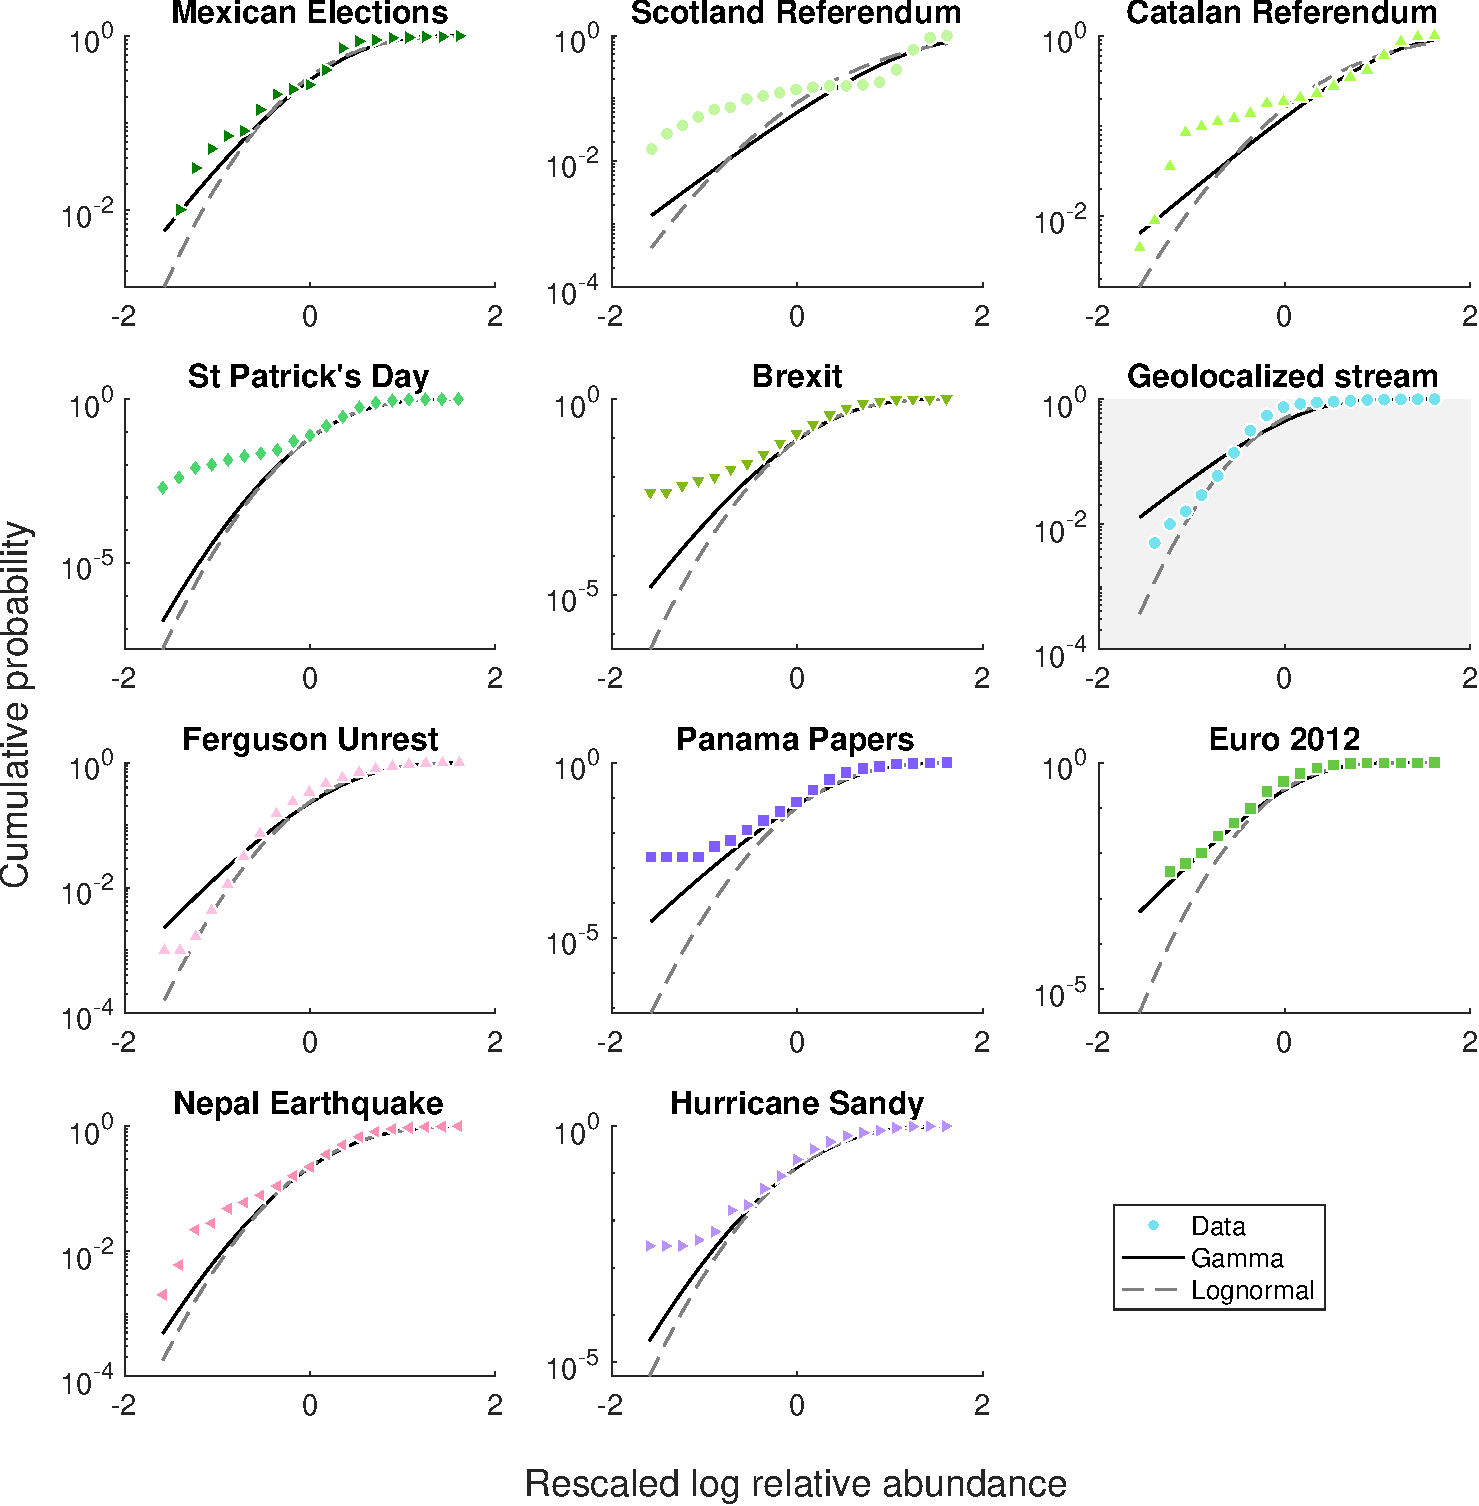
\includegraphics[width=\textwidth]{figures/chp4/AFD_tweet_RemSam.pdf}
    \caption[AFD]{AFD: Across each dataset, the distribution of abundances share a common shape. The datasets are sorted by the total number of different hashtags in ascending order. Greenish markers belong to expected events, pinkish to unexpected events. The sample which does not belong to any event (UK random) is in blue and hereinafter highlighted in gray for comparison. Relative abundances are rescaled to have zero mean and variance of one per bin.}
    \label{fig:4:AFD}
\end{figure}

Large abundances are particularly well described with these distributions. And among the parts that deviate from the distributions, the most usual feature is that small abundances are lower than expected. This indicates that hashtags have less extremely low abundances and could be a finite-size effect since the fluctuations in abundance are constrained by the finite amount of posts per bin. Interestingly, we find a complementary tendency in ecological data: the skewness is less than that expected, implying fewer extremely high values \cite{halley2002lognormality}. \\



%Among all the patterns, the AFD presents the highest variability, as some hashtags that are not the most abundant present other functional forms (see Figure X). The deviations may be a consequence of their hashtags frequencies, realization sizes, and of course, the existence of underlying generative processes.

Next, the mean relative abundance of hashtags across the bins in which datasets are divided scales with their variance following a power law (Figure~\ref{fig:4:TAY}): Taylor's law. An exponent close to $2$ arises consistently in all our datasets, suggesting that hashtags in online social networks follow a common dynamics that does not depend on either particular discussions or their size. The fit of Taylor's law exponents is shown in Table~\ref{tab:chp4:taylor}, where it can be observed that they are very similar. \\



\begin{table}[h] 
\caption{Estimated exponents across datasets for Taylor's law.}
\centering
\begin{tabular}{l c c c c } 
\hline 
Dataset &  $\alpha$ & $95\%$ CI & R \\ \hline \hline 
Mexican Elections & 1.895 & (1.857, 1.933) & 0.840 \\ \hline 
Scotland Referendum & 1.957 & (1.878, 2.036) & 0.610 \\ \hline 
Catalan Referendum & 1.874 & (1.816, 1.932) & 0.817 \\ \hline 
St Patrick's Day & 1.906 & (1.869, 1.943) & 0.689 \\ \hline 
Brexit & 1.858 & (1.826, 1.890) & 0.751 \\ \hline 
Geolocalized stream & 1.942 & (1.880, 2.004) & 0.718 \\ \hline 
Ferguson Unrest & 1.818 & (1.779, 1.856) & 0.804 \\ \hline 
Panama Papers & 1.812 & (1.686, 1.938) & 0.865 \\ \hline 
Euro 2012 & 1.933 & (1.823, 2.043) & 0.879 \\ \hline 
Nepal Earthquake & 1.865 & (1.848, 1.882) & 0.841 \\ \hline 
Hurricane Sandy & 1.882 & (1.864, 1.900) & 0.835 \\ \hline 
\end{tabular} \label{tab:chp4:taylor}
\end{table} 


%\begin{figure}[t]
 %   \centering
  %  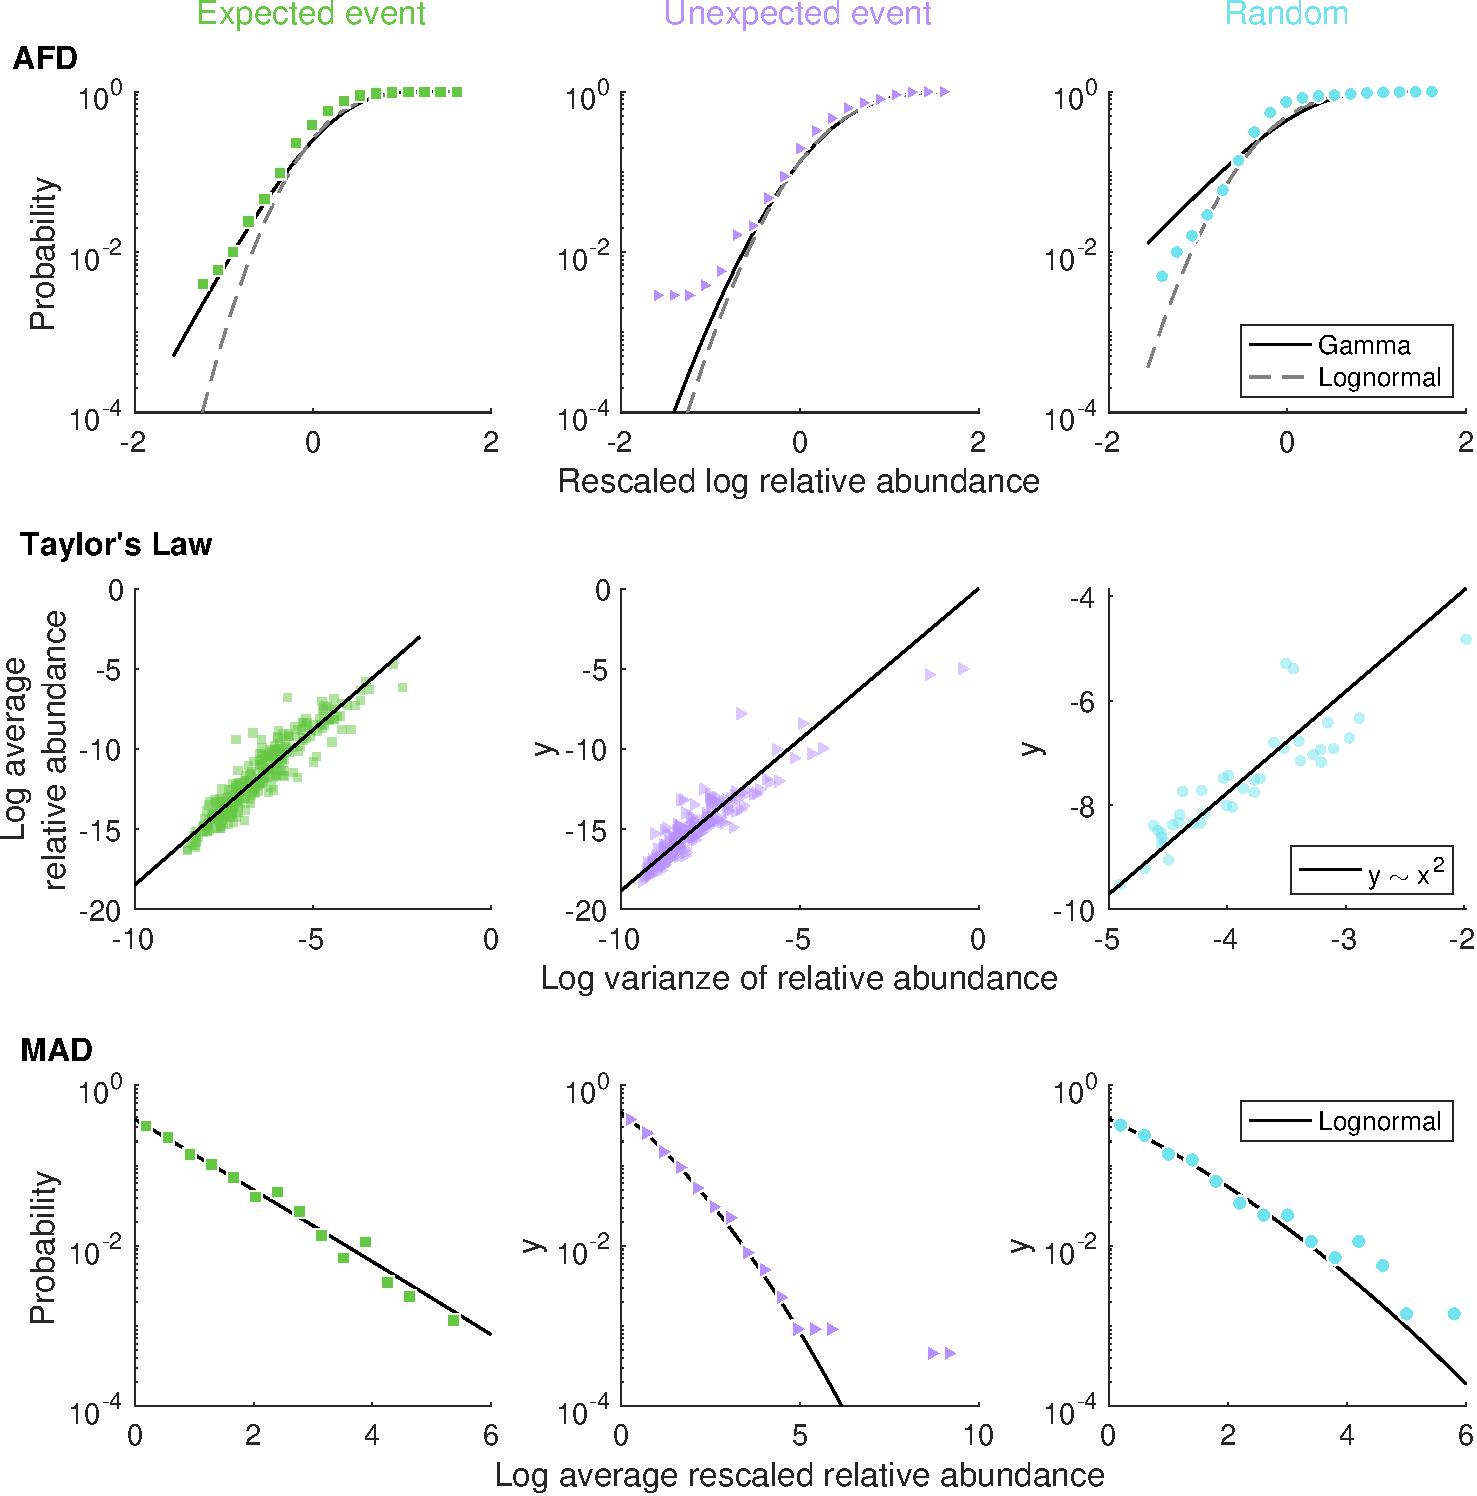
\includegraphics[width=\textwidth]{figures/chp4/Figure_Patterns1.pdf}
   % \caption[AFD, Taylor's law and MAD]{Caption}
    %\label{fig:AFD_TAY_MAD}
%\end{figure}

\begin{figure}[h!]
    \centering
    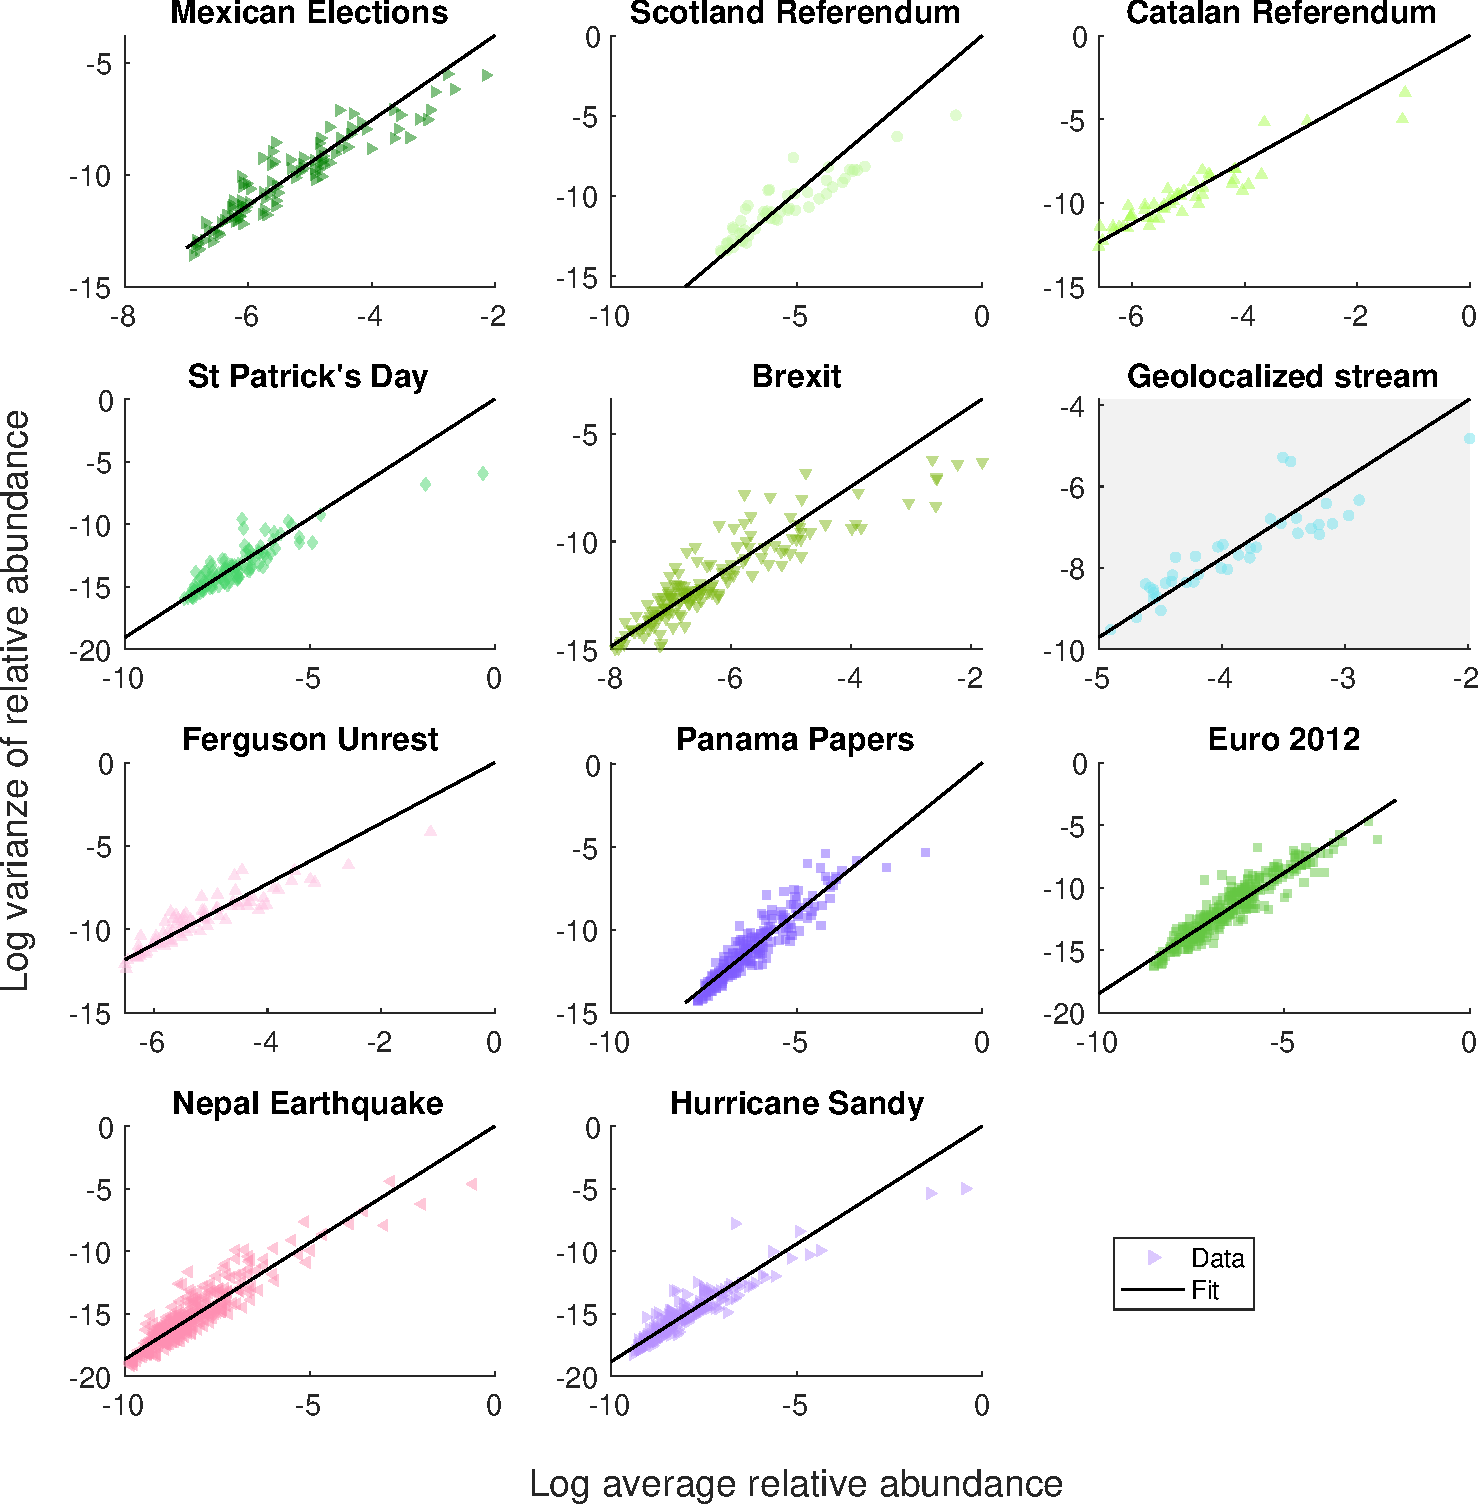
\includegraphics[width=\textwidth]{figures/chp4/TAYLOR_tweet_RemSam.pdf}
    \caption[Taylor's law]{Taylor's law: The variance of the abundance of hashtags over bins increases with the mean relative abundance as a power law of the from $\sigma_h^2 \sim \overline{x}_h^{\alpha}$. This relationship is consistent among all datasets with similar exponents. In the Panels, each point represents a hashtag. }
    \label{fig:4:TAY}
\end{figure}

Moving to the next pattern, when we plot the distribution of mean relative abundances (MAD), we observe that a lognormal distribution is compatible with them in all datasets (Figure~\ref{fig:4:MAD}). The shapes of the distributions vary from dataset to dataset, but a lognormal form is the best fit for all the datasets although with different values of $\mu$ (Table~\ref{tab:MAD}), like in ecological and microbial communities. General distributions in patterns like MAD and AFD, which remain consistent despite differences in details, can be applied in models to incorporate variability in their parameters. For example, the carrying capacity \cite{grilli2020macroecological} or food-webs interactions \cite{anderson1982variability} would not be constant, but random variables drawn from the corresponding distributions. Even though this approach would not capture all the variability of these parameters, it would still be more realistic than completely ignoring it. \\

 \begin{figure}[ht!]
    \centering
    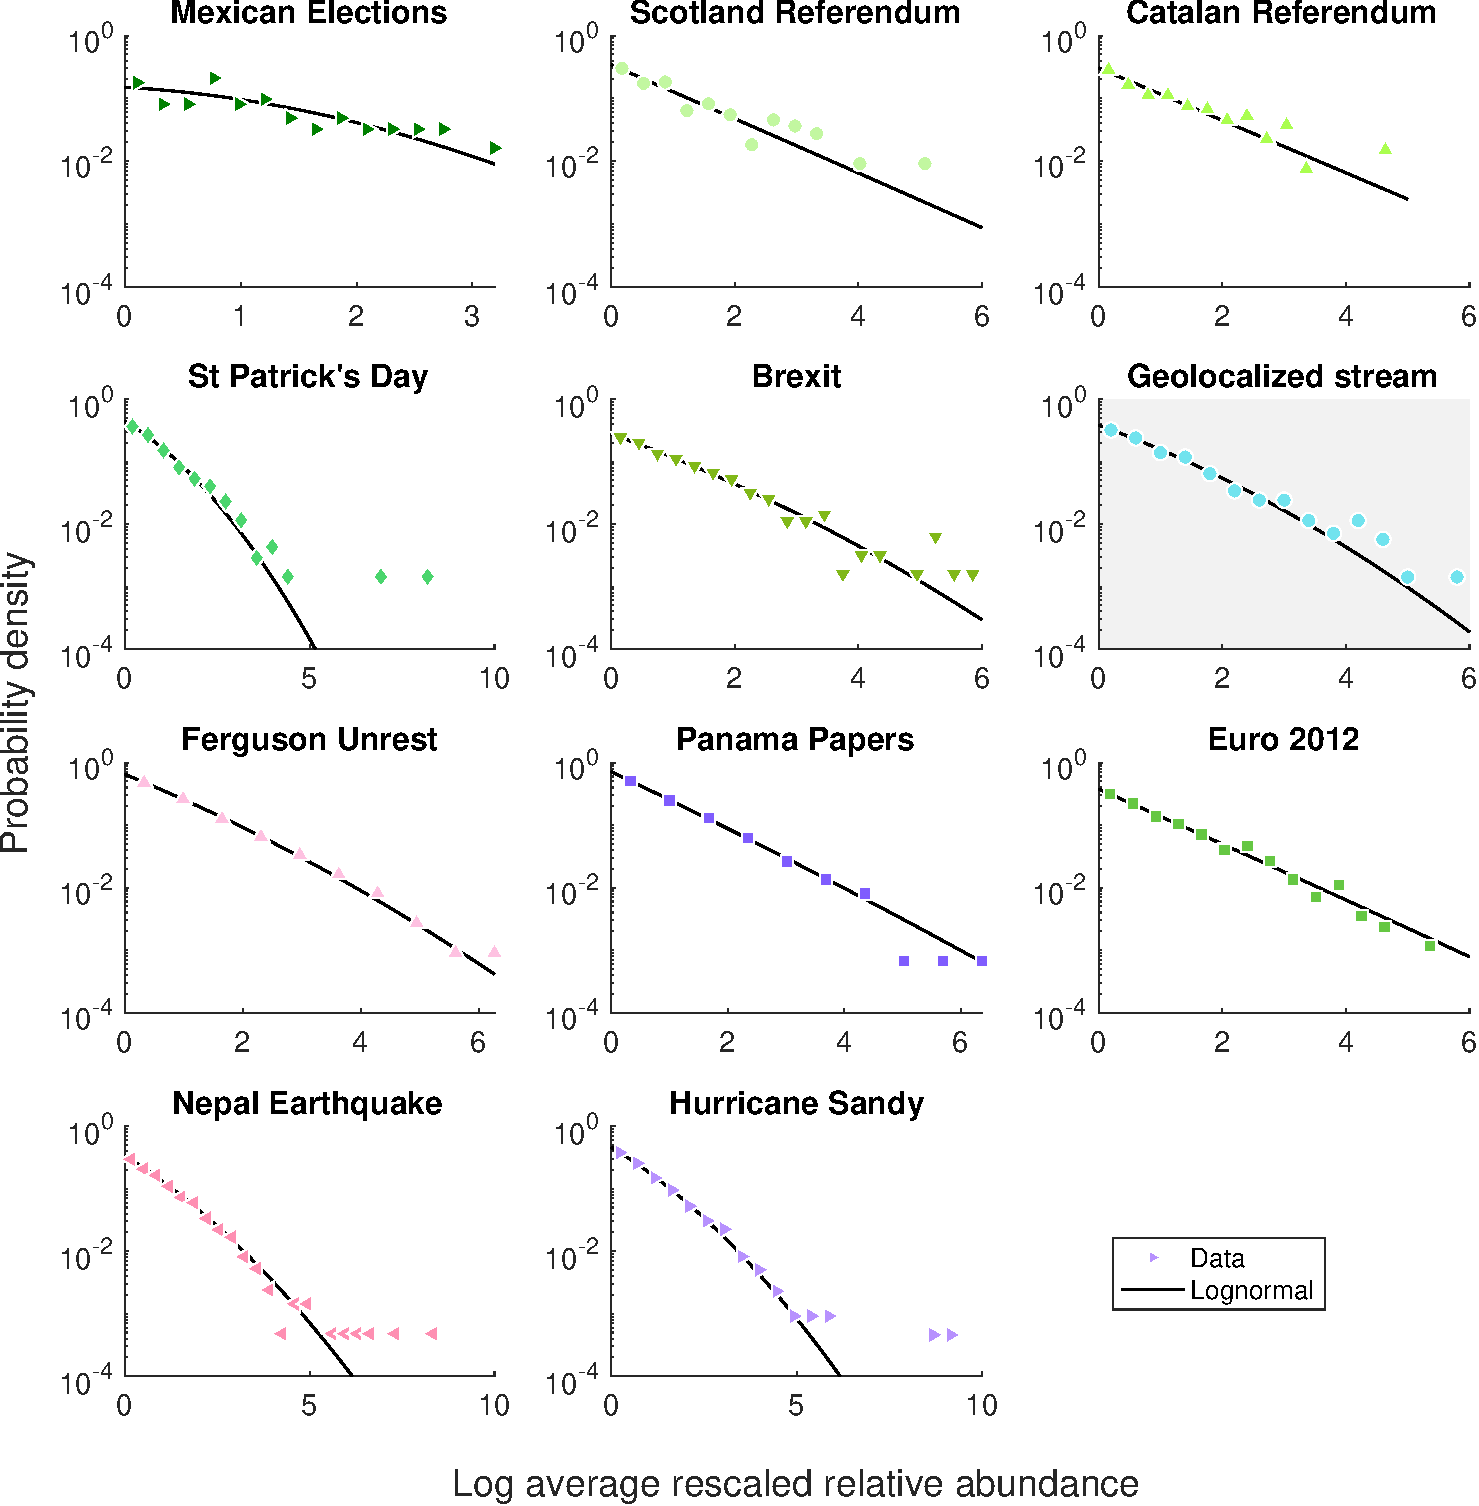
\includegraphics[width=\textwidth]{figures/chp4/MAD_tweet_RemSam.pdf}
   \caption[MAD]{MAD: The fit of the mean abundances closely follows a lognormal distribution. It is only performed over the positive values of their logarithm because the empirical MAD shows a lower cutoff established by sampling. The cutoff is based on the possibility that rare hashtags will never be found in a finite number of samples \cite{grilli2020macroecological}.}
    \label{fig:4:MAD}
\end{figure}

Moreover, a feature that we only see in some datasets related to events is that the most abundant hashtags have a mean relative abundance higher than dictated by lognormality.  Interestingly, the random-sampling dataset does not have this fat tail, indicating that it may be a sign of other processes going on in the former datasets that inflates certain hashtags.\\
%There is also a remarkable resemblance between these distributions and the frequency distribution of hashtags over the whole system, which means that the process generator of the abundances does not dilute the information about the recurrence of hashtags. Then, in a dataset with a high number of uncommon hashtags, we expect to find a high number of low-abundance hashtags.

For the species-accumulation curve (SAC), all the datasets present some part of the power-law relationship characteristic for intermediate scales (Figure~\ref{fig:4:SAC}). Some of them also start to saturate, meaning that we have sampled a considerable part of the discussion in those cases. The theoretical prediction for this pattern (Eq.~\ref{eq:SAC}) overall matches the empirical trends.\\


 %Within most natural communities, only a few species constitute the majority of the individuals and lots of species are in small numbers. That is, there are numerous rare species and only a few abundant species, making the relative species abundance distribution (RSA) highly skewed \cite{preston1948commonness,brown1995macroecology}. The RSA patterns have been well described with binomial or lognormal distributions, which are grounded in the theoretical framework of the neutral theory of ecology \cite{hubbell2001unified,volkov2007patterns}. These functional shapes depend on the type of scale considered, intrinsically connecting the RSA with the SAC \cite{azaele2016statistical}.
 In turn, the distribution of the abundance of hashtags (RSA) is consistent across all datasets and resembles the two proposed ecological distributions. There are few common hashtags with high abundance, but lots of hashtags are very uncommon. The same sweked RSA has also been found in some human communication systems such as emails, texts, and Twitter conversations \cite{tovo2021upscaling}. \\
 
 Remarkably, the UK random dataset, where there is not any main discussion to which those abundant hashtags can belong,  follows the same pattern as event-related datasets. Being that robust, a deviation from this trend could help in providing an estimate of the number of hashtags, and hence discussions, that a social network could host. \\


\begin{figure}[h!]
    \centering
    \includegraphics[width=1.1\textwidth]{figures/chp4/SAC_tweet_RemSam.pdf}
    \caption[SAC]{SAC: The species-accumulation curve for all datasets has a similar growth. Small points are bins, each of which with a different number of tweets (a proxy of scale). Larger points are averages over }
    \label{fig:4:SAC}
\end{figure}


\begin{figure}[h!]
    \centering
    \includegraphics[width=\textwidth]{figures/chp4/RSA_tweet_RemSam.pdf}
    \caption[RSA]{RSA: The probability of hashtags having a certain abundance follows a consistent form across all the datasets. It is plotted on a logarithmic scale, where each interval is twice the preceding one, following the classic work of \cite{preston1948commonness}. }
    \label{fig:4:RSA}
\end{figure}

For the STAC all the datasets reproduce a Laplace distribution (Figure~\ref{fig:4:STAC}). The abundance changes in our datasets share two common characteristics with the STAC of ecological communities: they are remarkably symmetrical and their mean $u$ tends to zero (Table~\ref{tab:STAC}). Thus, exactly as many hashtags are decreasing their abundance as they are increasing over the  recorded period. Such a pattern is compatible with a symmetric and zero-sum game as a generative mechanism for the data. Specifically, this zero-sum game is related to species competing for a finite set of resources \cite{marquet2005scaling,ji2020macroecological}. Moreover, it has been proven that the dynamics going on is compatible with a zero-sum game where the resource the different actors are competing for is the finite attention of the users \cite{gleeson2014competition,plata2021neutral,palazzi2021ecological,calleja2021quantifying}, so this pattern reaffirms with our current understanding of human behavior in online social networks.\\

Finally, it is worth mentioning another connection between the distribution of temporal changes in ecological and human systems. If the population mean abundance (MAD) follows a lognormal distribution, the STAC is theoretically expected to be Gaussian distributed. Even though the MAD of these systems is compatible with a normal distribution, a Laplace distribution for the STAC has been found not only in nature but also in artificial scenarios such as human institutions, from the growth rates of companies to countries’ gross national
product \cite{marquet2005scaling}. This ubiquitous presence suggests the existence of universal principles governing the growth dynamics of complex adaptive systems that are engaged in acquiring, transforming, and storing information, materials, or energy. \\


\begin{figure}[t]
    \centering
    \includegraphics[width=\textwidth]{figures/chp4/STAC_tweet_RemSam.pdf}
    \caption[STAC]{STAC: The distribution of temporal fluctuations fits with the Laplace distribution also found in ecological and social settings.}
    \label{fig:4:STAC}
\end{figure}


\section{Multinomial random sampling}
Once we have demonstrated that information ecosystems present the same universal laws observed in natural ecosystems, we go one step further in trying to understand their origin. In particular, there are two key ingredients to explain the emergence of patterns. One of them is discovering how the frequencies of each hashtag are generated. Why do we have a few very abundant hashtags and lots of rare hashtags? The second ingredient is determining how users choose what hashtags to post. We focus only on this latter aspect and generate synthetic communities with the same features as the observed ones but based on a null model. Specifically, we employ multinomial sampling. Starting from the hashtags' frequency distribution this method \cite{lego} generates random bins. We then calculate the same patterns from these resampled random bins and compare their characteristics with the original patterns (Figure~\ref{fig:4:randomSampling}).
%This method generates new bins by only assuming that hashtags appear randomly according to a fixed frequency. 
Besides, the model is neutral, which implies that all hashtags are equal in the eyes of the user.\\

Regarding how the model is implemented, we can replicate an empirical bin $b$ creating a random sample (with replacement) of size $N_b$, in which the probability that a set of hashtag abundances $ \{n_{h}\}$ occurs is given by:
\begin{equation}
    P(n_1, ... , n_H, N_b, f_1, ... , f_H) = \frac{N_b!}{\prod n_h!} \prod f_h^{n_h}
    \label{eq:multinomial}
\end{equation}
 where the frequency of a hashtag in the whole dataset is $f_h = \frac{1}{N} \sum_{b=1}^B n_{hb}$, and hence the probability of a new hashtag extraction is proportional to its global abundance $\sum_{b = 1}^B n_{hb}$. By doing this resampling for every bin of a dataset, we obtain a new random abundance matrix with the same size of the original one.

\begin{figure}[t]
    \centering
    \includegraphics[width=0.8\textwidth]{figures/chp4/randomSampling.pdf}
    \caption[Multinomial random sampling of posts]{Resample procedure: for every empirical dataset, we have calculated the hashtag frequencies and used them to resample each bin conserving the total number of hashtags found originally there.}
    \label{fig:4:randomSampling}
\end{figure}

\subsection{Confronting patterns}
By comparing the empirical patterns to the prediction generated by the multinomial random sampling, we can determine whether other factors besides hashtag frequency are driving the hashtag sampling. To do so, we have created $20$ resampled abundances matrices from our largest dataset and plotted their distributions together with the empirical ones in Figure~\ref{chp:4:fig:Lego}.\\

The analytical predictions based on Eq.~\ref{eq:multinomial} for some patterns (in Appendix~\ref{appen:patterns:eqs}) already tell us that an exponent one in Taylor's law is expected, which is precisely what we found with resampled data. Regarding the MAD, the multinomial data perfectly matches the frequency distribution (Figure~\ref{fig:appen:LegoAux}), which in turn remains close to the empirical distribution of mean abundances. Since the empirical MAD also reproduced the frequency distribution up to some extent, it is not a relevant pattern to distinguish deviations related to other processes and constraints in the datasets. This same reasoning can be applied to the RSA and SAC. The patterns that deal with distributions of fluctuations --AFD and STAC-- are expected to be more sensitive to external factors. In fact, for the AFD, the resampled distributions in Figure~\ref{chp:4:fig:Lego} present in general a higher probability of fluctuations. For the STAC, on the other hand, the short-term fluctuations are smaller than the empirical counterpart. Besides, in resampled bins, the dispersion of Taylor's law and SAC is reduced. However, this is not something remarkable since the random sampling has no exogenous noise. \\

Regarding the theoretical fits, some  patterns of the resampled bins have the same  peculiarities as the empirical patterns for online social networks: the AFD is fatter than the theoretical functional forms for small abundances --see Figures~\ref{fig:4:AFD} and~\ref{fig:appen:LegoAux}-- and both RSA present heavy tails --see Figures~\ref{fig:4:RSA} and~\ref{fig:appen:LegoAux}. \\

 %Multinomial AFD. The new bins are created with a different number of instances, accordingly to the bin from which we have taken the hashtags' frequencies, so a Binomial fit is not expected.

\begin{figure}[t]
    \centering
    \includegraphics[width=\textwidth]{figures/chp4/Figure_Lego_Hurricane Sandy_25Apr_lines.pdf}
    \caption[Macropatterns with the multinomial random sampling model]{Macropatterns obtained by the multinomial random sampling model for the largest dataset (Hurricane Sandy) confronted with the original patterns, in colored dots. Each gray line corresponds to a resampling of the entire dataset.}
    \label{chp:4:fig:Lego}
\end{figure}

\section{Implications of finding macropatterns}
%%%%%%%%%%%%%%%%%%%%%%%%%%%%%%%%%%%%%%%%%%%%%%%%%%%%%%%%%%%%%%%%%%%%%%%%%%

In this Chapter, we have found that six patterns originally discovered in ecological communities also hold for online social networks. These patterns not only are present in a variety of different datasets, but also their functional forms and parameters are compatible with the ones found in ecology. These common characteristics can help to guide the search for the underlying processes that create the patterns in the first place. \\

To expose the drivers, we have begun by comparing the empirical patterns with the patterns generated by a null model fed just with the frequency of hashtags in the online social network \cite{lego}. We find that some patterns are incompatible with this simple process, invalidating the assumption that hashtags are used solely based on their frequency and pointing to the existence of general laws in these systems. In particular, three patterns are informative about the fundamental mechanisms behind the observed behavior: Taylor's law, which is the pattern that shows clearly a divergence from a multinomial process, followed by deviations of the AFD and STAC.\\

Even though the resolution and number of our datasets are limited, systematically finding the patterns for all of them makes our results nevertheless quite convincing. Each dataset has been generated by an intrinsically-imperfect sampling, but since we have included datasets with different sampling methods, the possible biases are reduced. Regarding the theoretical functional forms borrowed from ecology, they are based on assumptions that may be revisited to fully characterize the driving processes in online social networks. Moreover, given that the processes at the origin of our patterns --regardless of which they are-- consistently manifest themselves in the predicted forms, it is crucial to have a robust method for fitting the empirical data to the theoretical distributions \cite{leroi2020neutral}. Searching for these patterns --and other ecological patterns not covered here-- in more datasets and fitting them with alternative methods can give more hints about how online social networks operate at the macroscopic level. \\

The proposed ecological-social bridge is strengthened by finding these common patterns, which also opens the door to benefit from the existing body of theory developed in the study of macroecological patterns. Specifically, macropatterns have had important predictive power in ecology \cite{brown1995macroecology} that can be put to work for social systems \cite{tovo2021upscaling}. If we have characterized a set of patterns for OSNs, the presence of exogenous factors that threaten their health can be uncovered by looking at any deviation from the natural form of these patterns. With our analyses, we have found that Taylor's law, AFD, and STAC are sensitive to the underlying processes, making them promising candidates for detecting external interference in the usual dynamics of online social networks.

\chapter{Conclusions}\label{chp:conclu}

In conclusion, we offer a comprehensive overview of our most significant findings and their implications. Our research has focused on the emergent behaviors that arise from the interactions among the components of complex systems, specifically ecological communities, and online social networks. Divided into two parts, the thesis examines each type of system, using a common approach that borrows concepts and models from ecology. In both parts, we study similar problems regarding coexistence but at different scales. We begin each part at the individual level by characterizing the effect of the spatial locations in Chapter~\ref{chp:1}, and quantifying interaction strengths in Chapter~\ref{chp:3}. We then increase our scale of description and study persistence at the species level in Chapter~\ref{chp:2}. In Chapter~\ref{chp:4}, we  deepen our abstraction to seek shared statistical patterns between social and ecological systems. Through the common ecological approach, we provide a unified framework for understanding the mechanisms that govern both ecological and information ecosystems. By bringing these systems together, we offer a more comprehensive understanding of the complex mechanisms that underlie their behavior. \\

Starting with the effect of spatial locations, Chapter~\ref{chp:1} models individuals competing in different spatial substrates. These spatial effects are thought to be one of the most prevalent mechanisms at play in real ecosystems \cite{Dieckmann2000}. Consequently, it is crucial to include space in the analysis of competitive communities, where stable coexistence cannot be achieved through intransitivity alone \cite{soliveres2018everything,godoy2017intransitivity,Grilli2017Higher-orderModels}. Our research suggests that local interactions promote stability by effectively reducing inter-species competition and damping large fluctuations in species abundances. In this sense, a limited interaction range cancels out the neutral oscillatory behavior characteristic of mean field models of intransitive interactions. Even though our results were derived from a simple model,  this Chapter adds a new perspective on how space can stabilize competitive communities. \\

While Chapter~\ref{chp:1} deals with interactions at the individual level, mechanisms of coexistence can also operate at the species level \cite{Grilli2017,Garcia-Callejas2018ThePersistence}. This is why we increase the scale of research in Chapter~\ref{chp:2} and look at the architecture of the species interactions. At the scale of species, an important question for persistence has been to explain why some species go extinct \cite{Sole2001, Keyes2021AnLosses}. We investigate how the network structure determines the probability of species survival after an environmental change when we consider multiple interaction types. The effect of network architecture has been extensively studied, but often focusing only on ecosystems' food webs and ignoring other interactions \cite{pascual2006ecological,kefi2020theoretical}. In this Chapter, we have taken into account two non-trophic interactions --competition and mutualism-- first in isolation and then simultaneously. We have addressed this challenge by simulating a dynamics embedded in the interaction network, and then by analyzing the structural properties of surviving species through machine learning. We have found that two node metrics that regard centrality are the main predictors of extinction. In mutualistic communities, species with low eigenvector centrality are more prone to extinction when all the interactions' strengths have been modified due to an environmental perturbation. In a competitive scenario, the same role is played by a high Page-Rank. However, when we model both interactions at the same time, predictors are not universal and vary with the structure of each community and the interaction strengths. The Chapter aimed to overcome some simplifications that have been used when modeling ecological interaction networks. Typically, only one type of interaction is usually addressed and, when the focus of the work is on structural analysis, the effect of the dynamics is neglected.  However, ecological communities are complex systems, and the results of studying multiple interactions together might not be the same as when they are studied separately \cite{kefi2012more,Kefi2015NetworkShores}. We have addressed mutualism and competition, but any other type of interaction, like predator-prey or parasitism, could be further included, together with  allometric-inspired dynamics, to improve realism. Nevertheless, as a consequence of the results of this work, we are now in a position to highlight the significance of revisiting classic results of interactions in isolation, which bring us closer to the ultimate goal of addressing ecological coexistence. \\

%Chapter 4:
%But networks are inherently difficult to understand, as
%the following list of possible complications illustrates...
%To make progress, different fields have suppressed certain
%complications while highlighting others. -> sim plified For instance, in nonlinear
%dynamics we have tended to favour simple, ...

% As a take-home message, when we study communities with both types of interactions, predictors are not universal and vary with the structure of each community and the interaction strengths. As a consequence of the results of this work, we are now in a position to highlight the significance of revisiting classic results of interactions in isolation, which bring us closer to the ultimate challenge of studying several interactions simultaneously to better understand ecosystems.

During the second part of the thesis, we maintain our pursuit of discovering mechanisms for coexistence, but we shift our focus to a slightly different system: online social networks. However, we do not abandon the ecological jargon and concepts from the first part. Instead, we leverage the similarities between ecological and social systems and approach the latter as information ecosystems. In this social context, 
we have addressed the drivers of collective attention, since it is crucial for understanding how to conserve the diversity and health of our information ecosystems \cite{palazzi2021ecological, gleeson2016effects}. In Chapter~\ref{chp:3},  we proposed a methodology to measure
the intensity of competitive and mutualistic interactions between users and hashtags based on Lotka-Volterra equations and niche theory. Our results show that during events that captivate collective attention, users experience reduced net competition. Then, the agreement between the
data and the numerical simulations suggests that the seek for visibility is what drives users’ behavior: users who participate in online debates tend to increase their visibility within the themes that interest them, creating intense competition inside each topic. The same visibility maximization encourages agents to follow the dominant topic as an event approaches, raising competition but also expanding viewers. This rearrangement of interactions is stable, however, because mutualistic benefits outweigh the more intense competition. \\

 Our results in Chapter~\ref{chp:3} shed light on one of the mechanisms behind the emergence of collective attention in online social media. The optimization of visibility and the consequences that we have found operate at the microscopic level, guiding the decisions of individual users. To unravel more mechanisms, in Chapter~\ref{chp:4} we have again scaled up our approach and studied the relationships between the agents of an information ecosystem, this time going to the broadest of perspectives, by characterizing and explaining statistical patterns of diversity and abundance. This task is also taken through an ecological perspective, to profit from the body of theory and philosophy that have been already developed in the study of macroecological patterns \cite{brown1995macroecology}. We have detected that the universality of ecological patterns found in both macroecological systems and microbiological communities is conserved in information ecosystems: i.e. even the same functional forms  of natural ecosystems are found in online social networks. Furthermore, as previously mentioned, identifying patterns is useful to construct theories and models, but equally valuable is identifying where these patterns are broken \cite{lego}. If a universal pattern is not present in a specific circumstance, it could indicate the presence of additional factors that are preventing the natural distribution from forming. This can have direct applications in information ecosystems, particularly when evaluating their health. For instance, a missing or distorted pattern may be the consequence of external interference, like bots disseminating misinformation. Understanding the general shape of these patterns may allow us to detect these threats more effectively, ultimately protecting the democratic discourse. As a result, one of the contributions of this thesis is in  fostering how an ecological perspective on the study of information ecosystems may offer practical resources for understanding social and collective processes.\\

 %This thesis has explored diverse aspects of the persistence of ecological communities and emergent phenomena in information ecosystems. Despite the approaches taken may seem pretty different --besides being inspired by ecology-- the chapters share a common viewpoint: they develop models to better explain, describe or predict empirical phenomena. While it is true that the various models emphasize different causal forces, this should be regarded as a benefit since their implications and insights overlap and interweave \cite{page2018model}. During this thesis, we have developed multiple models that operate at different scales for the same general goal. For example, we described a competitive dynamics through spatial networks of individuals in Chapter 3, and through a community network at the level of species in subsequent Chapter~\ref{chp:2} to study the emergence and maintenance of coexistence. The central idea behind our work is that by employing different models we can develop a nuanced and deep understanding to gain insights that may have otherwise been obscured. Models are just representations that can be expressed through mathematics and logic. All models share two common characteristics: simplification, which involves stripping away unnecessary details or abstracting from reality; and formalization, which uses precise definitions and mathematical expressions to represent the underlying concepts. By using different models, we emphasize some forces (space in Chapter~\ref{chp:1} or the species interactions in Chapter~\ref{chp:2}) while we simplify others (all species compete with  one another in Chapter~\ref{chp:1} and there are no spatial effects in Chapter ~\ref{chp:2}). Given that ecological --and complex-- systems function at multiple scales, it is only by collecting varied and even potentially contradictory sets of narratives that we can ultimately arrive at a more complete understanding. \\

In this thesis, we have explored diverse aspects of the persistence of ecological communities and emergent phenomena in information ecosystems. Even though we have developed different models, we can do it through the lens of complex systems. We have begun by using a sort of toy model in Chapter~\ref{chp:1}, which functions primarily as a mathematical representation, enabling us to state hypotheses and delve into their implications \textit{in sicilo}. As we progress through the thesis, we introduce more and more complexity and information by incorporating empirical data. Simulations are run on artificial and real network structures in Chapter~\ref{chp:2} to prove that theoretical results on systems with only one interaction type should be revisited. In Chapter ~\ref{chp:3}, a model inspired by Lotka-Volterra equations allows us to lay out the hypothesis that the driver of collective attention is users' visibility optimization, and its consequence is an increment in competition for attention. The importance of using data in this Chapter increases, since by using that model along with empirical data, we then are able to test and validate our hypothesis. The last Chapter of the thesis heavily relies on empirical data to identify patterns to provide a conceptual understanding of online social networks as information ecosystems. These patterns can be useful for generating hypotheses, inspiring models, or providing insights into complex phenomena that we would not have imagined looking at the raw data alone. As Dostoyevsky writes in \textit{Crime and Punishment}: ``We’ve got facts, they say. But facts aren’t everything; at least half the battle consists in how one makes use of them!''. Our patterns' description in Chapter~\ref{chp:4} reveals the statistical invariants that arise from the underlying drivers of information ecosystems (the facts) and paves the way for proposing new theories about their functioning. Given that ecological --and complex-- systems function at multiple scales, it is only by collecting a varied set of narratives through simulation and data that we can ultimately arrive at a more complete understanding.\\

%Furthermore, as mentioned earlier, not all models serve the same purposes. While the models of the first three Chapters can be regarded as more or less simple toy models, Chapter~\ref{chp:4} used a more descriptive approach. Toy models function primarily as a mathematical representation, enabling us to state hypotheses and delve into their implications in great detail. In Chapter ~\ref{chp:3}, for instance, a vitaminized model inspired by Lotka-Volterra equations allows us to lay out the hypothesis that the driver of collective attention is users' visibility optimization, and its consequence is an increment in competition for attention. By using the same model and empirical data, we then were able to test and validate our hypothesis. This empirical data is precisely what the other type of model employed in this thesis, the descriptive model, requires. The description of the patterns in Chapter~\ref{chp:4} aims to provide a conceptual understanding of online social networks as information ecosystems and relies on empirical data to identify those patterns. Descriptive models can then be useful for generating hypotheses or providing insights into complex phenomena that we would not have imagined looking at the raw data alone. As Dostoyevsky writes in \textit{Crime and Punishment}: ``We’ve got facts, they say. But facts aren’t everything; at least half the battle consists in how one makes use of them!''. Our patterns description in Chapter~\ref{chp:4} reveals the statistical invariants that arise from the underlying drivers of information ecosystems (the facts) and paves the way for proposing new theories about their functioning. \\

%Finally, we wish to emphasize the interdisciplinary nature of this thesis, which is evident in both the topics explored and the tools utilized. Our research addressed a range of subjects such as competition for space, ecological communities, and collective attention in social systems. To address these complex topics, we employed a variety of tools and techniques, like network theory, nonlinear dynamics, data analysis, and machine learning. All of these methods are linked by their ecological approach. Through our results, we shed light on how users' behaviors in social media are driven by information processing and, they highlight the opportunities that an ecological approach can present to the understanding of collective phenomena in social systems. In a broader sense, this thesis contributes to the integration of a complex-system philosophy in the study of both social and ecological systems. Our hope is that the examples presented here will inspire future research on ecology and computational social science with the foundations and applications of complex systems.

Finally, this thesis takes an interdisciplinary approach to exploring complex systems in both ecological and social settings. Through a range of subjects such as competition for space, survival in ecological communities, and collective attention in social systems, we employed a variety of tools and techniques, like network theory, nonlinear dynamics, data analysis, or machine learning. Our results shed light on how users' behaviors in social media are driven by information processing, and demonstrate the opportunities an ecological approach can present to the understanding of collective phenomena in social systems. The contributions of this thesis extend beyond our specific research and contribute to the integration of a complex-system philosophy in the study of both social and ecological systems. Our hope is that the examples presented here will inspire future research on ecology and computational social science with the foundations and applications of complex systems.

%lazer2020computational? 


 % TO CONCLU Our results throw light on how users' behaviors in social media are driven by information processing and, in a broader sense, they highlight the opportunities that an ecological approach can present to the understanding of collective phenomena in social systems. \\
 

%---------------------------------------------------------------------------
%	APPENDICES
%---------------------------------------------------------------------------
\singlespacing
% the back matter
\clearpage
\phantomsection
%activate only when we finish.
\begin{appendices}

\chapter{Some node metrics}\label{chp:methods:predictors}
Throughout the thesis, several node properties are used to characterize either the behavior of the system (as the average degree in Chapter~\ref{chp:1}) or the entities that nodes represent (as we will see in Chapter~\ref{chp:2}). The list of properties presented here is far from complete in terms of literature, but describes all the tested metrics in Chapter~\ref{chp:2}. The references include their definitions and relevant ecological works in which they appear. 
\subsubsection{Centrality metrics:}
\begin{description}
 \item[Degree:]  It measures how many nodes a node is connected to. 
   \begin{equation}
   k_i = \sum_j A_{ij}
   \end{equation}
   where $A_{ij} = {0,1}$.  \\
   References: \cite{Newman2010},\cite{Gouveia2021},\cite{Jordan2008IdentifyingNetworks}  
   \item[Betweenness centrality:] It measures the extent to which a node lies on paths between other nodes. \\
   References:    \cite{Newman2010} , \cite{Estrada2007CharacterizationSpecies}, \cite{Gouveia2021}, \cite{Jordan2008IdentifyingNetworks} \item[ Closeness centrality :]  It measures the mean distance
from a node to other nodes.   \\
   References:  \cite{Newman2010} ,\cite{Gouveia2021},\cite{Jordan2008IdentifyingNetworks}
\item[Eigenvector centrality:]  It measures how well-connected a node is to other well-connected nodes. It is the
leading eigenvector of the adjacency matrix $A$.  \\
   References:   \cite{Newman2010}, \cite{Allesina2009GooglingCoextinctions} ,\cite{Estrada2007CharacterizationSpecies} 

\item[PageRank:] 
   PageRank was originally designed as an algorithm for ranking web pages' search results. It is based on the number and quality of the neighbors and is proportional to how often a random walker visits the target node.\\
   References:   \cite{Langville2006ARetrieval}, \cite{McDonald-Madden2016UsingEcosystems}  

 \end{description}
 \subsubsection{Meso-scale metrics:}
 \begin{description}
     
\item[ k-core :] It is a set of nodes where each is connected to at least $k$ others.   \\
   References:  \cite{Newman2010}, \cite{Morone2019TheEcosystems} 
\item[ Rich Club :] For each node of degree $k$, its rich-club coefficient is the ratio of the number of realized links to the number of potential links with nodes whose degree is greater than $k$. \\
   Reference:   \cite{McAuley2007Rich-clubHierarchies}  
\item[Clustering Coefficient  (CC):]  It is the ratio of the number of pairs of neighbors of a node to the total number of pairs of neighbors of that node.    \\
   References: \cite{Newman2010},\cite{Estrada2007CharacterizationSpecies} 
\item[ Average neighbor degree  (Avg. Neig. k) :]  
 It is the average degree of the neighborhood of a node.  \\
   Reference:  \cite{Barrat2004TheNetworks}  
   \end{description}

\subsubsection{Signed Metrics:}
   \begin{description}
       
\item[Strength:] 
It has been observed a positive correlation between strong interaction strengths in a few plant species and an increment in community diversity \cite{melian2009diversity}.
\begin{equation}
       \textrm{strength}^{i}_{tot} = \sum_j A_{ij}
\end{equation}
 when $A$ is weighted.  \\
   References: \cite{Jordan2008IdentifyingNetworks},\cite{melian2009diversity}
\item[ Relative Interaction  Index:]  It measures the dominant interaction sign for each node independently of the size of the network.
\begin{equation}
    RII = \frac{k_+ - k_-}{k_+ + k_-} 
\end{equation}
\item[ Relative Balance  Index:] It measures the dominance of balanced or unbalanced triads independently of the network size:
\begin{equation}
     RBI = \frac{B - U}{B + U},
\end{equation}
where $B$ ($U$) is the number of balanced (unbalanced) triads a node participates in. 
Reference: \cite{harary1955local}
\item[PN-centrality:] It is a centrality measure for signed networks introduced in \cite{everett2014networks}. Let $n$ be the total number of nodes, $P$ the adjacency matrix of only the positive links of the network, $N$ that of only the negative links, and $A = P-2N$. PN centrality is defined by the expression:
\begin{equation}
    PN = \left(I_n - \frac{1}{2n-2}A\right)^{-1} \mathbb{1},
\end{equation}
where $\mathbb{1}$ is the vectors of all ones. The implications of this formula are not yet completely understood, but the measure has become standard in the social network literature.
\item[Generalized PageRank (GPR1):]  AS an alternative to PN centrality, we introduce two signed versions of PageRank. Let $n$,$P$, and $N$ as before, and let $D$ be the diagonal matrix of total degrees (positive plus negative). Now let $A = (P-N)D^{-1}$, and let $\alpha \in (0,1)$ be a damping factor. Our first signed version of PageRank is defined by the formula:
\begin{equation}
 GPR_1 = (I_n-\alpha A)^{-1} \mathbb{1},
\end{equation}
where $\alpha = 0.85$. The intuitive ideas behind this formula are that the effect of a node $i$ on an adjacent node $j$ is inversely proportional to the total degree of $j$, with the sign of the effect being that of the sign connecting $i$ to $j$. This effect is multiplicative along paths and damped by a factor $\alpha^k$ along paths of length $k$. A truncated version of this measure, considering only paths up to a certain length, was introduced in \cite{liu2020simple}.
\item[Generalized PageRank (GPR2):] Our second generalization is a variation of the previous GPR1 where now $D$ is the diagonal matrix of the absolute difference between the positive and negative degree of nodes. In that way, nodes with a large difference between positive and negative links are more penalized.
\end{description}
\chapter{\label{appen:MF}Analytical formulation for structured interactions}

Along with a numerical implementation of the dynamics described in Chapter~\ref{chp1:1}, it is
also possible to provide a mathematical description of the
model, which we set up in this Appendix. In Section
\ref{sec:moments} we establish the basic equations for the
moments of the population variables. Section~\ref{sec:mf}
develops a standard mean-field approximation for statistically
homogeneous systems. We stress that it is not able to reproduce
the main numerical findings for our model, but gives a baseline
to interpret the results. Section~\ref{sec:localmf} extends the
mean-field approximation to allow for spatial inhomogeneity in
the species distribution. The results still do not match with
the numerical observations, but give some hints on the reduced
stability of homogeneous oscillations when the interaction
range is small.

\subsection{Moment equations}
\label{sec:moments}

An analytical description of the stochastic dynamics defined in
the main text can be given (after a trivial replacement of the
discrete-time dynamics by a continuous-time one) by the master
equation for the time-dependent probability of the system
state. It allows us to derive equations for the expected
relative abundance of each species at a given node as well as
for the two-node correlations.

The model state can be specified by giving $\{Z_\nu\}$, where
$Z_\nu=1,2,...,g$ specifies the species that occupies node
$\nu\in\Sigma$, with $\Sigma$ being the set of nodes of the
network. However, we find more convenient to parameterize the
model as follows. Let $n_{i,\nu}\in \{0,1\}$ be the number of
individuals of species $i\in\{1,\dots,g\}$ at node $\nu\in
\Sigma$, i.e. $n_{i,\nu}=1$ for one and only one $i$,
identifying the species present at $\nu$, and $0$ for the other
values of $i$ (absent species). The state of the system can be
characterized by the set of vectors $S=\{S_\nu\}_{\nu=1}^N$,
with $S_\nu=\{n_{1,\nu},\dots,n_{g,\nu}\}$. This state evolves
as follows: (i) with a rate $r$, a randomly chosen individual
(say, located at $\nu$) dies, then (ii) two neighbors of the
dead individual (thus pertaining to the set $P_\nu$ of
neighbors of $\nu$) are chosen at random and compete to
generate the offspring: a winner species is selected according
to the probabilities in the dominance matrix $H$. And (iii)
this offspring is immediately located at the vacant node.
Following standard procedures (for example see
 \cite{khlohe17,klkh20}) the master equation for the probability
$p(S,t)$ of finding the system in a state $S$ at time $t$ can
be written as
\begin{align}
  \label{eq:me}
  \frac{\partial}{\partial t}p(S,t)=
  \sum_{\nu=1}^N\sum_{i,j}\left( E^+_{i,\nu}E^-_{j,\nu}-1\right)\pi_\nu(i\to j)p(S,t),
\end{align}
where the operators $E^\pm$ act on an arbitrary state function
$f(S)$ as
\begin{eqnarray}
  \nonumber
E^\pm_{i,\nu}f(S)=f&\Big(&\{n_{1,1},\dots,n_{g,1}\} ,\dots, \\   \nonumber
&&\{n_{1,\nu},  \dots,n_{i,\nu}\pm 1,\dots,n_{g,\nu}\},\dots,\\
&&  \{n_{1,N},\dots,n_{g,N}\} \ \ \Big).
\end{eqnarray}
$\pi_{\nu}(i\to j)$ is the rate at which an individual of
species $i$ is replaced by one of species $j$ at site $\nu$,
given by
\begin{equation}
  \pi_{\nu}(i\to j)=r\frac{n_{i,\nu}}{N}\frac{2}{k_\nu(k_\nu-1)}
  \sum_{\stackrel{\lambda,\mu\in P_\nu}{\mu\neq \lambda}}\sum_{k}n_{j,\lambda}n_{k,\mu}H_{jk},
\end{equation}
where $k_\nu$ is the degree of node $\nu$, i.e. the number of
nodes in $P_\nu$. 


From the master equation we can derive equations for the
moments of the distribution, which can be easily measured from
the numerical simulations. The simplest nontrivial moment is
the expected number of individuals of species $i$ at node
$\nu$, $\mean{n_{i,\nu}}$. Its equation is readily obtained
from the master equation after multiplying it by $n_{i,\nu}$
and summing over all possible values of $S$:
\begin{eqnarray}
  \label{eq:ni}
  \frac{d}{ds} \mean{n_{i,\nu}} =&& \frac{1}{k_\nu(k_\nu-1)}
  \sum_{j} \sum_{\stackrel{\lambda,\mu\in P_\nu}{\mu\neq \lambda}}
  H_{ij} \mean{n_{i,\lambda}n_{j,\mu}}\nonumber \\
  && - \frac12 \mean{n_{i,\nu}} ,
\end{eqnarray}
where we have introduced a new time scale $s\equiv
\frac{2r}{N}t$.

From this equation we can write the dynamics for the expected
value of the macroscopic variable $x_i(s) \equiv N^{-1}\sum_\nu
n_{i,\nu}$ as 
\begin{equation}
\label{eq:xintermsofP}
  \frac{d}{ds} \mean{x_i(s)} =
  \sum_{j} H_{ij} P_{ij}(s) - \frac12 \mean{x_i(s)} ,
\end{equation}
where we have introduced the symmetric matrix
\begin{equation}
\label{eq:Ps}
  P_{ij}(s) = \frac{1}{N} \sum_\nu \frac{1}{k_\nu (k_\nu -1)}
  \sum_{\stackrel{\lambda,\mu\in P_\nu}{\mu\neq \lambda}} \mean{n_{i,\lambda}n_{j,\mu}} \ .
\end{equation}
This matrix can be interpreted as the probability of sampling
at time $s$ a pair of individuals of species $i$ and $j$ when
deciding the replacement of a dead individual somewhere in the
system. It satisfies  $\sum_{ij} P_{ij}(s) =1$
and, in a homogeneous network ($k_\nu=k$, $\forall \nu$),
$\sum_{j=1}^g P_{ij}(s)=\mean{x_i(s)}$.


As for the second-order moments, both for $\mu \in P_{\nu}$ and
for $\mu\notin P_\nu$, their equations read
\begin{eqnarray}
\nonumber
  \frac{d}{ds} \mean{n_{i,\nu}n_{j,\mu}} =&&\frac{1}{k_\nu(k_\nu-1)}
  \sum_{l}\sum_{\stackrel{\delta,\lambda\in P_\nu}{\delta\ne \lambda}}H_{il}\mean{n_{i,\lambda}n_{l,\delta}n_{j,\mu}} \\
  && + \frac{1}{k_\mu(k_\mu-1)}
  \sum_{l} \sum_{\stackrel{\delta,\lambda\in P_\nu}{\delta\ne \lambda}}H_{jl}\mean{n_{j,\lambda}n_{l,\delta}n_{i,\nu}} \nonumber \\ &&-\mean{n_{i,\nu}n_{j,\mu}}.
\label{eq:ninj}
\end{eqnarray}

In general, it can be seen that the moment equations form a
hierarchy, namely that the equation for a moment of order $o$
depends on the moments of order $o+1$. Hence, they cannot be
solved in closed form, except if introducing some
approximation.

\subsection{Homogeneous mean-field approximation}
\label{sec:mf}

The simplest of such approximations is the mean-field approach.
It is conveniently done in the simplified case in which the
network is spatially homogeneous, i.e. all the nodes have the
same degree: $k_\nu=k$, $\forall \nu$. In this situation, we
can search for statistically homogeneous solutions:
$\mean{n_{i,\nu}(s)}=\rho_i(s)$, $\forall \nu$. We can relate
these time-dependent moments $\rho_i(s)$ to the macroscopic
variables $x_i(s) \equiv N^{-1}\sum_\nu n_{i,\nu}(s)$ (note
that $\sum_{i=1}^g x_i(s)=1$). Indeed we have
$\mean{x_i}=N^{-1}\sum_\nu \rho_i=\rho_i$, or
$\mean{x_i}=\mean{n_{i,\nu}}$.

The mean-field approximation, which is exact in the case of
all-to-all interactions in an infinite system, and expected to
be accurate both for large enough interaction range (mean
degree) and for unstructured interactions, consists in
neglecting fluctuations and correlations:
\begin{eqnarray}
& \mean{n_{i,\nu}}=\mean{x_i}  \simeq x_i\ ,  & \forall \nu\in \Sigma, \\
& \mean{n_{i,\nu} n_{j,\mu}}   \simeq \mean{n_{i,\nu}} \mean{n_{j,\mu}} \simeq x_ix_j \ , &  \forall \nu\ne \mu \in \Sigma.
\end{eqnarray}
We have also $P_{ij}\approx x_i x_j$. Introduction of these
expressions into Eq. (\ref{eq:ni}) leads to a closed evolution
equation for $x_i$:
\begin{equation}
  \label{eq:meanf}
  \frac{d}{ds} x_i = \left(\sum_{l}H_{ij}x_j-\frac12\right)x_i \ .
\end{equation}

This mean-field equation has been studied before (e.g.
 \cite{Grilli2017Higher-orderModels}). We summarize here the
main results:

First, the dynamics (\ref{eq:meanf}) maintains in time the
property $\sum_i x_i =1$, if the initial condition satisfies
it. This can be seen by defining $X\equiv \sum_i x_i$,
calculating $dX/ds$, using that $H_{ij}=(H_{ij}+H_{ij})/2 =
(1-H_{ji}+H_{ij})/2$, and noticing that $\sum_{ij}
(H_{ij}-H_{ji})x_i x_j =0$ and $\sum_{ij} x_i x_j =X^2$. Thus
the sum of relative abundances satisfies
\begin{equation}
\label{eq:sumdynamics}
\frac{dX}{ds} = \frac12 (X^2 - X) \ ,
\end{equation}
which maintains $X(t)=1$, $\forall t$ if
$X(0)=1$.

Second, Eq. (\ref{eq:meanf}) has several equilibria or fixed
points. Many of them are of the `absorbing' or `boundary' type,
i.e. steady solutions of (\ref{eq:meanf}) in which $x_i=0$ for
some $i$, so that the corresponding species are extinct. In
addition, if $g$ is odd, there is generically
 \cite{Grilli2017Higher-orderModels} an \textit{interior}
equilibrium, $x_i(t)=x_i^*$, $\forall t$, in which all species
coexist with non-vanishing relative abundances $x_i^*$. At this
fixed point the relative abundances are given by
\begin{equation}
  \label{eq:sts}
  \sum_{j=1}^g H_{ij} x_j^* =\frac12 \ \ \Rightarrow \ \
  x_i^*=\frac12 \sum_j (H^{-1})_{ij},
\end{equation}
where $H^{-1}$ is the inverse of the dominance matrix, which
always exists when it describes an intransitive loop. The
properties of the boundary fixed points can be analyzed by
recognizing that they can be considered interior equilibria in
a system with a smaller number $g$ of species.

Third, the dynamics from arbitrary initial conditions in which
all $x_i$ are non-vanishing (and for generic $H$) leads to a
transient in which some of the species may become extinct. The
remaining ones, an odd number, cycle neutrally around the
interior fixed point (\ref{eq:sts}) in which the rows and
columns corresponding to the extinct species have been removed
from $H$ \cite{Grilli2017Higher-orderModels}. The stability of
this interior equilibrium is always neutral: relative
abundances of surviving species describe periodic closed orbits
around it, with an amplitude and period that is determined by
the initial condition and without being attracted nor repelled
by the fixed point. This can be seen
 \cite{Grilli2017Higher-orderModels} by noticing that the
quantity
\begin{equation}
V(x_1,...,x_g) = - \sum_{i=1}^g x_i^* \log \frac{x_i}{x_i^*}
\end{equation}
is a constant of motion, and thus it foliates the
$(g-1)$-simplex on which the dynamics occurs into invariant
hypersurfaces that turn out to contain concentric closed orbits
around the interior equilibrium.

The neutral character of the oscillations is not realistic from
the biological point of view, and structurally unstable from
the mathematical point of view. It is a consequence of the mean
field approximation, and we expect such neutral cycling to be
broken under corrections to mean-field, or under the full
dynamics with finite range of interaction. This is indeed what
is seen in our numerical simulations for the full model with
three species: either the fixed point becomes attracting, or
the neutral cycles are replaced by a single attracting limit
cycle, with amplitude and period independent of the initial
conditions.

In addition to its non-robust prediction of neutral cycling of
the species, the mean-field approximation is not able to
explain our main numerical finding: the fixed point
becomes stable for short-range interactions. From the
observations of Section~\ref{chp1:2.3} and Figure
\ref{chp1:fig:5} it is likely that the stabilization of the
fixed point arises from the fact that the relative abundance
$x_i$ are macroscopic quantities that become averaged and
non-fluctuating when the microscopic structure contains many
different domains, as in Figure \ref{chp1:fig:5}a. Thus,
it is pertinent trying to extend the mean-field formalism to
describe the microscopic spatially-dependent configurations, as
done in the following section.


\subsection{Local mean-field and spatial stability}
\label{sec:localmf}

In this section we consider the species locations to be at the
nodes of a two-dimensional square lattice. Then the node index
$\nu$ can be considered to be a discrete two-dimensional vector
$\nu$. For regular networks such as this one, the mean-field
approximation can be made local in space. This involves
removing correlations as
$\mean{n_{i,\mathbf{\nu}}n_{i,\nu}}\simeq\mean{n_{i,\nu}}\mean{n_{i,\nu}}$
while keeping the dependence of the mean quantities on the node
location.

Under this approximation, Eq.~\eqref{eq:ni} can be written as:

\begin{dmath}
 \frac{d}{ds}\rho_i(\nu,s) =  \frac{1}{k(k-1)} \sum_{j} H_{ij}  \left[
  \left(\sum_{\lambda\in P_\nu}\rho_i(\lambda,s)\right) \left(\sum_{\mu\in P_\nu}\rho_j(\mu,s)\right)
  - \sum_{\lambda \in P_\nu} \rho_i(\lambda,s) \rho_j(\lambda,s)
  \right]   -\frac{1}{2}\rho_i(\nu,s).
\label{eq:localMF}
\end{dmath}

We have used the notation $\mean{n_{i,\nu}} \equiv
\rho_i(\nu,s)$. Note that this equation reduces to Eq.
(\ref{eq:meanf}) when $\rho_i$ is homogeneous:
$\rho_i(\nu,s)=x_i(s)$, $\forall \nu$.

This new formulation allows us to assess the stability of
particular solutions against spatially-dependent perturbations.
For example we can focus on the stability of an homogeneous but
time-dependent solution $\rho_i(\nu,s)=x_i(s)$ which verifies
Eq.~\eqref{eq:meanf}. To do so, we seek a solution to
Eq.~\eqref{eq:localMF} of the form
\begin{equation}
  \rho_i(\nu,s)=x_i(s)+\delta_i(\nu,s),
\end{equation}
and linearize to first order in $\delta$. With this,
Eq.~\eqref{eq:localMF} becomes


\begin{dmath}
\frac{d\delta_i(\nu,s)}{ds} = \sum_j \frac{H_{ij}}{k}
\left[ x_j(s) \sum_{\lambda\in P_\nu} \delta_i(\lambda,s)
+  x_i(s) \sum_{\lambda\in P_\nu} \delta_j(\lambda,s)\right]  -\frac12 \delta_i(\nu,s)  \ .
\label{eq:localMFlin}
\end{dmath}

We introduce the Fourier transform of the perturbation:
$\hat\delta_i(q,s) = \sum_\nu e^{i q\cdot\nu}
\delta_i(\nu,s)$, in terms of which Eq.
(\ref{eq:localMFlin}) reads:
\begin{eqnarray}
  \frac{d\hat\delta_i(q,s)}{ds} &=& \left[ -1 + 2 F(q) \sum_j H_{ij} x_j(s) \right]\hat\delta_i(q,s) \nonumber \\
                                &+& F(q) x_i(s) \sum_j H_{ij} \hat\delta_j(q,s) \ .
\label{eq:stability}
\end{eqnarray}
We have introduced the quantity
\begin{equation}
  \label{eq:fourarA}
  F(q)\equiv \frac{1}{k}\sum_{\lambda \in P_{0}} e^{iq \cdot \lambda} \ ,
\end{equation}
which satisfies $F(q = 0)=1$, $|F(q)|\le 1$, and
$F(q)\to 0$ as $|q|\to \infty$. Note that this quantity
contains information on the interaction range through the
dependence on $P_{{0}}$ (i.e. through the set of neighbors of the origin). 
%{\VC DEFINE $P_{\bm{0}$}.

The simplest case to analyze is the stability of the interior
equilibrium point, i.e. $x_i(s)=x_i^*$, $\forall s$ as given by
Eq.~\eqref{eq:sts}. In this case Eq. \eqref{eq:stability} is a
linear system with constant coefficients, hence the stability
depends on the eigenvalues of the matrix of coefficients
$M_{ij}=F(q)x_i^* H_{ij} + [F(q)-1]\delta_{ij}/2$.  In
fact, because of Eq. (\ref{eq:sumdynamics}), there is always an
unstable eigenvalue $1/2$ for perturbations that bring the
dynamics out of the simplex. Thus, it is convenient to restrict
the dynamics to the simplex by using $\sum_{j=1}^g \delta_j=0$,
and then the matrix of the coefficients of Eq.
(\ref{eq:stability}) restricted to the first $g-1$ dimensions
is $M_{ij}=F(q)x_i^* (H_{ij}-H_{ig}) +
[F(q)-1]\delta_{ij}/2$, $i,j=1,...,g-1$.

For example, for $g=3$, the two eigenvalues of $M$ restricted
to the simplex can be explicitly calculated and read
\begin{equation}
  \lambda_\pm=-\frac{1-F}{2}
  \pm i \frac{F}{2}\sqrt{\frac{(2H_{12}-1)(2H_{13}-1)(2H_{23}-1)}{1 - 2(H_{12}-H_{13}+H_{23})}} \ .
\end{equation}
The argument of the square root is always positive when $H$
presents intransitive dominance cycles. Hence
\begin{equation}
  \textrm{Re}[\lambda_\pm]=-\frac{1-F(\mathbf q)}{2}\le 0
\end{equation}
and the equality holds if and only if $\mathbf q=\mathbf 0$.
This means that, within the mean-field approximation, the
steady and homogeneous solution $\rho_i(\nu,s)=x_i^*$ is 
linearly stable against small spatial perturbations, except for
homogeneous perturbations, in which stability is marginal (a
fact that we already knew from the more general nonlinear
arguments in Section~\ref{sec:mf}). Thus, the local mean-field
dynamics of Eq. (\ref{eq:localMF}) leads, for inhomogeneous
initial conditions close to the interior fixed point, to a
homogenization of the configuration, which then proceeds to
cycle neutrally around the fixed point. This is confirmed by
direct numerical simulation of Eq. (\ref{eq:localMF}). These
results hold for any value of the interaction range, contained
in $F(q)$. Thus, this local mean-field theory is not able to
explain the results from our stochastic model with structured
interactions. Namely, a transition from persistent inhomogeneous
configurations at short interaction range, which produce a
fully attracting fixed point for the macroscopic variable
$x_i(s)=\sum_\nu \rho(\nu,s)$, to a situation with
oscillatory dynamics that produces a repelling fixed point and
limit-cycle oscillations for $x_i(s)$ at large interaction
range.

Nevertheless, we can still use the local mean-field to gain
further insight into the dynamics, for example by analyzing the
stability with respect to inhomogeneous perturbations of a
homogeneous periodic solution $x_i(s)$ of Eq. (\ref{eq:meanf}).
In this case the stability equation (\ref{eq:stability}) is a
linear equation with periodic coefficients, which can be
analyzed with Floquet theory. The solutions can be written as a
linear combination of the functions \cite{gl94}
\begin{equation}
  f_i(s)e^{p_i s},\qquad i=1,\dots,g-1,
\end{equation}
where $f_i(s)$ are periodic (and hence bounded) functions of
time, with the same period $T$ as the functions $x_i(s)$, and
$p_i$ are the Floquet exponents given in terms of the
eigenvalues $\Lambda_i$ of the fundamental matrix $\Phi(s)$ of
system \eqref{eq:stability}, satisfying $\Phi(0)=I$, as
\begin{equation}
  \Lambda_i=e^{p_i T}.
\end{equation}
When all $p_i$ are negative, the perturbations decay and the
homogeneous solution $x_i(s)$ is recovered as time advances. We
have numerically evaluated $p_i$ for the case of three species,
$g=3$, and some values of the parameters of the system. For all
cases considered, $p_i$ has always negative real parts (except
for homogeneous perturbations, for which one finds neutral
stability), meaning that any initial inhomogeneous perturbation
tends to disappear. This agrees with direct simulation results
of Eq. (\ref{eq:localMF}). Thus, the long-term behavior of the local mean-field approach 
reduces to the standard homogeneous mean-field
treatment of Section~\ref{sec:mf}. In contrast, simulation of the
stochastic model shows domains of the different species for
short interaction range.

However, the stability strength is not the same for all
parameter values. Let $M(s)$ be the matrix of time-dependent
coefficients of the system \eqref{eq:stability}. A necessary,
but not sufficient, condition for the homogeneous solutions
$x_i(s)$ to be unstable is that some eigenvalue of $M(s)$ has
positive real part for some time $s\in[0,T]$  (see a proof of a
similar result in \cite{klkh20}). During these times, even if
the trajectory turns out to be linearly stable, its stability
is reduced and more susceptible to non-infinitesimal
perturbations or noise. For the case of three species $g=3$,
and the interaction matrix $H$ given again by Eq.~(\ref{eq:H}), we have seen
that the matrix $M(s)$ has eigenvalues with positive real
parts, for some possible periodic trajectories $x_i(s)$,
provided $F(q) \gtrsim 0.67$. Since the maximum of $F(q)$
occurs at zero wavenumber and the width of this function
decreases with increasing $k$, the band of wavenumbers
identified as `less-stable' shrinks as the interaction range,
quantified by $k$ increases. This is an indication (although
not a proof) that homogeneous periodic solutions would be more
robust for long-range interactions, and instabilities giving
rise to inhomogeneous configurations are more likely to occur
for short-range interactions. It is interesting to note that the
times at which the matrix $M(s)$ has more positive real-part of
eigenvalues coincide with the times at which some of the
components of the oscillatory solution $x_i(s)$ approach zero.


On general grounds, the local mean-field approximation should
represent some kind of coarse-graining of the original
stochastic system, and should be completed by noise terms to
gain accuracy. Under short-range interactions, appropriate
noise terms would be able to break the synchronization between
distant locations, and reproduce the domain structure
observed in the Monte Carlo simulations. However, we find
difficult to write analytical expressions for these noise terms
that would respect all the proper statistical constraints (for
example: reflect the multiplicative nature of birth-death
fluctuations, keep in time that $\sum_i \rho_i(\nu,s)=1$,
etc.). Also, the complexity of such model would not be lower
than the original individual-based one. Thus, we have not
developed further this possibility. 
%{\VC Las referencias se salen de la pagina}


\section{\label{sec:app_toymodel} Introducing correlations 
beyond mean-field}

In section \ref{chp1:2.3} we demonstrated that short-range interactions lead to the emergence of mono-specific clusters, effectively increasing intra-specific competition and 
stabilizing the dynamics.  As a further way to confirm that the decline of  inter-specific
competition is able to change the stability of the equilibrium,
making it stable for sufficiently reduced competition between
distinct species, we have studied a toy-model which shares
characteristics with our community model. It is built by
noticing that $\langle P_{ij} \rangle$ is just the time average
of the matrix $P_{ij}(s)$ in Eq. (\ref{eq:Ps}).
A way to correct the mean-field approximation $ P_{ij} \approx
x_i x_j$ is to introduce some correlations, $ P_{ij} \approx
c_{ij}x_i x_j$, making some ansatz for $c_{ij}$ and introducing it
into the exact equation (\ref{eq:xintermsofP}) (with
$\mean{x_i}\approx x_i$). We have explored the behavior of such
model in which correlations are implemented by
$c_{ij}=1-\epsilon$ if $i\neq j$ and $c_{ii}=1+\epsilon'$, with $\epsilon,\epsilon'>0$, 
resulting in an enhanced intra-specific competition with respect to
 inter-specific competition as $\epsilon$ and $\epsilon'$ are
increased. With this choice of $c_{ij}$ the resulting matrix
$P_{ij}$ does not have the proper statistical properties. In
particular the model does not respect that $\sum_i x_i=1$,
$\forall s$. However, this problem can be fixed by
constraining the dynamics onto the simplex by subtracting to
Eq. (\ref{eq:xintermsofP}), for each species $i$, the same term
$g^{-1}\sum_i G_i$, where $G_i$ is the right-hand-side of Eq.
(\ref{eq:xintermsofP}). It should be clear that this is not a
systematic approximation to our original system, but a toy
model useful to check the impact of varying the intra- and inter-specific competition balance. For example, for
$\epsilon'=0.01$ and the same dominance matrix used in Chapter~\ref{chp:1}, we have found that a Hopf bifurcation occurs at
$\epsilon = \epsilon_c\approx 0.01975$, so that relative
species abundances undergo limit cycle oscillations for
$\epsilon<\epsilon_c$ but the fixed point becomes stable and
attracting when the inter-specific competition is further
reduced, $\epsilon>\epsilon_c$. These are the same type of
states and the same transition that is encountered in our
stochastic model when decreasing the interaction range.

\chapter{Calculating areas in the simplex}\label{appen:AreaSimplex}
In Chapter~\ref{chp:1}, we characterize the behavior of the competitive community by considering the area encircled by the system’s trajectory on the simplex. Because of the noisy character of the dynamics in the stochastic simulations, the amplitude of the oscillations is not a robust indicator. Instead, if the system fluctuates with small amplitude around some equilibrium abundances, the trajectory occupies a small area (Figure~\ref{chp1:fig:3}c), whereas larger oscillations would cover broader areas (Figure~\ref{chp1:fig:3}a,b). Here we add details on how we compute the area encircled by the trajectory.\\

We have run $50$ realizations of our $3$-species system for every radius. For each simulation, the trajectory can be interpreted as points in a 3D space (gray dots in Figure~\ref{fig:areaExplained}, where the averaged density triplet $(\overline{x}_1,\overline{x}_2,\overline{x}_3)$  is the middle cross). To characterize the trajectory, we aim to measure the area covered by those points. \\

For programming convenience, it is more practical to change to a two-dimensional space $(y_1,y_2)$. The chosen space is the one defined by the $x +y +z = 1$  plane, as the density triplets always lie on it because $\sum_{i}^{g} x_i(t) = 1$ at all times. Let $(\hat{u},\hat{v})$ be two vectors in that plane that form an orthonormal basis. In particular:
\begin{equation}
    \hat{u} = \sqrt{\frac{1}{2}} \begin{pmatrix}
           -1 \\
           1 \\
           0
         \end{pmatrix} , \;
    \hat{v} = \sqrt{\frac{2}{3}} \begin{pmatrix}
           -1/2 \\
           -1/2 \\
           1
         \end{pmatrix}.
\end{equation}
The areas in each space are conserved because the transformation is isometric. In turn, the change of coordinates of our points is given by:
\begin{equation}
    y_1 = (x_1,x_2,x_3)\sqrt{\frac{1}{2}} \begin{pmatrix}
           -1 \\
           1 \\
           0
         \end{pmatrix} , \;
     y_2 = (x_1,x_2,x_3)\sqrt{\frac{2}{3}} \begin{pmatrix}
           -1/2 \\
           -1/2 \\
           1
         \end{pmatrix}.
\end{equation}
During the simulation, heavy fluctuations may occur, but the densities there do not represent the typical behavior of the ecosystem. These extreme densities are the outermost points of the set of points that populate the two-dimensional space. To get a representative area, we eliminate those boundary points, more precisely, we remove the $5\%$ of outlier points. We then calculate the area enclosed by the polygon defined by the new outermost points (green line in Figure~\ref{fig:areaExplained}) using \texttt{MATLAB}'s function  \texttt{polyarea} \cite{polyarea}.

\begin{figure}
    \centering
    \includegraphics[width=\textwidth]{figures/appendices/area_explainedy.png}
    \caption[Calculating areas in the simplex]{Trajectory points in the $2$D of a simulation of a RGG with $10^4$ nodes and $R_{RGG} = 0.03$. The red line encloses all the points. Green and blue lines enclose the $95\%$ and $90\%$ of the points, respectively.}
    \label{fig:areaExplained}
\end{figure}

 
\chapter{Inferring empirical ecological networks: everything is biased}\label{appen:Inferring}
In Chapter~\ref{chp:2}, we used empirical ecological networks for our analysis. In the end, the validity of our results will depend on the quality of the data available, and therefore it is important to know some aspects of data collection. \\

The data to recreate an ecological network can be obtained through direct observations (like watching a visit of a certain pollinator to a given flower), indirect observations (like pollen analysis in insects' limbs), or inference (for example based on traits, like the famous Darwin's prediction of the existence of a moth with an enormous proboscis because of the existence of an orchid with extremely long  nectar tubes \cite{darwin1877various}). For the two latter cases, what we are doing is basing the interaction on a proxy. Every method, specifically the second and third one, poses some limitations that could compromise the applicability of our results. Thus, when using empirical networks like in Chapter~\ref{chp:2},  it is convenient to have in mind what are the hidden assumptions in the data collection. \\

We have worked with two different groups of ecological networks. One set has only mutualistic networks from the web service  \href{www.web-of-life.es}{``Web of Life''}. In general, the studies comprise the direct collection of floral and visitor species. A possible limitation of those datasets is the intensity of the survey, together with the presence of any agricultural or other human disruptors that may have stressed the habitat. Fortunately, if we take as a case study our largest dataset \cite{robertson1928flowers}, a second survey at the passage of $75$ years found that more than $82\%$ of the species are still found despite habitat changes \cite{marlin2001native}. \\

\begin{figure}[h!]
     \centering
\includegraphics[width=\columnwidth]{figures/methods/fig_hugofacitilation.pdf}
 \caption[Spatial co-occurrence networks]{(Panel a) The ecological interpretation of three spatially associated plants is that of a complete facilitation triad. (Panel b) Two species spatially coexist and the third one segregates for them, hence the negative links. Panels a and b adapted from \cite{Saiz2017EvidenceNetworks}.(Panel c) Visualization of the network $\texttt{Emp}\_\texttt{AE}$ from \cite{Saiz2017EvidenceNetworks}. Each node represents a species and the link color is the type of interaction: green for mutualism and red for competition.}
\label{chp:methods:fig:hugo}
\end{figure}

A more blatant assumption when working with these datasets is the fact that, since they do not record competition, we have supposed competition between guilds is a matter of shared mutualistic patterns. For example, if two pollinators visit the same flowers, they may be competing for the finite amount of nectar. However, in plants, it is not the most crucial competition factor. To overcome this possible limitation, we have also used empirical networks where the spatial distribution of plants determines their competitive interactions \cite{Saiz2017EvidenceNetworks}. Now, the spatial pattern is a proxy for plant competition. A significantly high spatial co-occurrence is a proxy for facilitation or mutualism (Figure~\ref{chp:methods:fig:hugo}a), and significantly low spatial co-occurrence indicates segregation (negative links), which is a proxy for competition in plants communities (Figure~\ref{chp:methods:fig:hugo}b).\\

Local spatial association between pairs of plant species determines the links and their interaction sign in these networks. But abiotic factors can also influence how plants distribute in space. For example, soil composition, sunlight, or underground water sources. Moreover, and in particular, in plant communities, the signs of interactions can change throughout the year \cite{losapio2019perspectives}. However, since the networks are constructed by dominant interactions, these facts should not affect them. Finally, it has been theoretically proven that the relationship between spatial segregation and competition can be reversed if diffusion or continuous niches are considered \cite{hernandez2009species}.  \\

Finally, a common feature of both the visiting and spatial association networks is that they are symmetric and connected. Regarding connectivity, species that are outside the giant component of the interaction network have usually less abundance and dominance, and their effect on the overall is predicted to be almost negligible for our purposes. Symmetry is, per contra, a more delicate issue because it has been recently hypothesized that another alternative key factor for stability in ecosystems could be precisely asymmetry on the interaction strengths \cite{allen2023structural}. 




%%%%%%%%%%%%%%%%%%%%%%%%%%%%%%%%%%%%%%%%%%%%%%%%%%%%%%%%%%%%%%%%%%%%%%%%%%%%%%%%%%%%%%%%%%%%%%%%%%%%%%%

\chapter{Decision trees}\label{appen:DT}
Decision trees are one type of machine learning classifiers \cite{loh2011classification}. They infer the correct class of an observation by a series of yes/no questions, the answer of each question determining the next to ask until a classification is made. These questions, also called rules, are about the values of the observation in a set of variables. We use decision trees in Chapter~\ref{chp:2} to infer whether a species in an ecological network (our observation) will survive or not (the classification) according to their structural properties (the set of variables). Decision trees are convenient for our problem since they do not impose any assumption on the training data, and handle several variables at the same time, even if they are correlated, as some network metrics are \cite{Pichler2022MachineEcologists}.  \\

A trained decision tree starts at a single node called ``root'' node (bottom node in Figure~\ref{app:fig:DT}), which represents a rule for a variable, and then branches in two directions. For example, Rule 1 is ``$k_- > 3$'' in Figure~\ref{chp2:fig:2}. An observation from the data goes to the  right branch of the node if it passes that threshold. Otherwise, it goes to the left. Therefore, each branch corresponds to different possible outcomes, and finishes on new nodes that incorporate more rules on variables until the final classification is achieved at the ``leaves''. \\

The most important variable in predicting the correct class could be deduced from the hierarchy of the nodes. That variable would be the root node, as it can divide the entire data. For example, in Figure~\ref{app:fig:DT}, one could say that the variable involving Rule 1 is the most important as that variable alone can already classify some observations in one class. This rough estimation can only tell us about one variable, and nothing about the following nodes that \textit{just} refine data subsets. However, we can quantify the importance of all the variables if we know some aspects of the training of a decision tree. Explaining this will be a small detour, but it will pay off. \\

\begin{figure}
    \centering
   \includegraphics[width=0.8\textwidth]{figures/appendices/DT.pdf}
   
    \caption[Parts of a decision tree]{Parts of a decision tree.}
   \label{app:fig:DT}
\end{figure}

The training of a decision tree is recursive, it follows the same steps for each node. To choose the root node, it scans each variable and tries to divide the training data based on it. Then, the decision tree evaluates each split in light of a ``splitting criterion'' to determine which one performs the best. The splitting criterion we have used is Gini impurity because it favors larger partitions \cite{growingdecisiontrees}. For each branch $b = \{1,2\}$ in a split involving variable $\alpha$, Gini impurity is defined as:

\begin{equation}
   G_b^\alpha = 1- (p_{sur}^2 + p_{ext}^2), 
   \label{eq:ginibalpha}
\end{equation}
where $p_{i}$ is the proportion of observations labeled with class $i = \{sur,ext\}$. We then weigh and sum the Gini impurities of all branches based on the proportion of the data each branch takes up, $d_b$.
\begin{equation}
    G^\alpha  =  d_1 G_1^\alpha + d_2 G_2^\alpha,
    \label{eq:ginialpha}
\end{equation}
where $d_1+d_2=1$. From Eq.\eqref{eq:ginibalpha}, we can see that if a variable can classify all its incoming observations with a single label (a perfect classification), its Gini impurity would be zero and the branch will finish with a leave. For example, the root node in Figure~\ref{chp2:fig:2} (and its schematic version, the Figure~\ref{app:fig:DT}) can directly label some species as ``Surviving''. For all the variables, the one with the smallest impurity will be chosen as the node. Returning to Figure~\ref{chp2:fig:2}, if we constrained the decision tree to just one node, choosing $k_-$ would be the variable that best classifies more species. The logic for all the following nodes is the same. \\

Once the decision tree is constructed, we find in the nodes variables that have a low Gini impurity. Using this concept, the importance $I$ of a variable can be defined as how much each split decreased the impurity. More precisely, it is the difference between the risk for the node (a.k.a. the parent node) and the total risk for its two children nodes \cite{importance}:
\begin{equation}
    I = R_{parent} - R_{child\,1} - R_{child\,2}
    \label{eq:importance}
\end{equation}
In turn, the risk of a node $R_\alpha$ is defined as its impurity weighted by the probability $f_\alpha$ that an observation falls into that node:
\begin{equation}
    R_{\alpha} = G_\alpha f_\alpha
\end{equation}
This probability is just calculated by dividing the number of observations that arrive at the node by the total number of observations in our training data. A node would score one, the maximum importance, if and only if it is the root node (so $f = 1$) and it perfectly splits the data on their labels ($G = 1$ and $R_{child\,1} = R_{child\,2} = 0$). 

Two situations can increase the risk of a node: having high impurity or having a large number of observations passing across it. Nodes at the beginning of a tree will have the highest $f_\alpha$ by definition. The children of these nodes, however, may have still a higher risk than children from nodes near the top that have more chances of a perfect classification. In that way, the importance is less controlled by the order in which nodes appear in the tree. Finally, the most important variable will be the one that minimizes the impurity the most effectively. \\

We can rank the variables according to their importance. But before accepting any ranking, we first need to assess the performance of the decision tree. Ultimately, if the algorithm does not classify the observations with good accuracy, the importance of their variables will the useless. To check the accuracy of the predictions, we create a confusion matrix (Panel a of Fig.\ref{chp2:fig:6}  and \ref{chp2:fig:8}). Its rows correspond to the true class a species belongs to and the columns to the class predicted by the decision tree. Hence, diagonal elements are the percentage of species that are correctly classified, while incorrect predictions are at the off-diagonal elements. \\

To improve the accuracy displayed in the confusion matrix, one could go on growing the tree more and more complex by increasing the number of branches. This would help to better classify the most subtle idiosyncrasies. But when presented with new data, the accuracy of this decision tree would drop. It has been adapted so much to the training data that its predictive power has begun to wane. This is called ``over-fitting'' and it is a crucial aspect of machine learning algorithms' design \cite{spiegelhalter2019art}. In Chapter~\ref{chp:2}, we will train our decision trees for particular types of networks, but we want the results to apply to those types as a whole. \\

There are good practices to avoid over-fitting  \cite{spiegelhalter2019art}. Without giving all the details, we start by randomly dividing our dataset into a training set and a test set. Generally, the training set comprises $80\%$ of the observations The accuracy of the decision tree is now evaluated at the test set, so we can check whether the decision tree is adapting too much to the local circumstances of the training set. A second idea that we have implemented in the construction of the decision tree is ``k-fold cross-validation'' \cite{crossval}. It builds on the idea of testing the algorithm with an independent set. The training dataset is randomly divided into $k$ sets of equal size. Then $k-1$ sets are chosen for training, and this step is repeated $k$ times. The final decision tree is a generalization of the $k$ trees. In this way, the quality of the classification improves since we are systematically removing observations during the construction. \\

Finally, the decision trees have been trained and validated using the \texttt{MATLAB R2021a} algorithms  \texttt{fitctree} \cite{fitctree} and \texttt{crossval} \cite{crossval} from its Statistics and Machine Learning Toolbox.
\chapter{Supporting results for structural predictors}\label{appen:SuppPredictors}

%Here we add some details on the supporting results of  Chapter~\ref{chp:2}.

\section{Persistence not equal to 50\%} \label{SI:1}
\begin{figure}[h]
    \centering
    \includegraphics[width=\textwidth]{figures/appendices/fig_Importance_mut_persisNOT50.pdf}
    \caption[Importance profile when persistence is not $50\%$]{Normalized importance for empirical network $\texttt{Emp}$\_$\texttt{IL}$ ($N = 1500$) with only mutualistic interactions when persistence is $30\%$ ($\alpha_+ = 0.05$) and $80\%$ ($\alpha_+ = 0.03$).}
\end{figure}

\newpage
\section{Metrics over time} \label{SI:2}
\begin{figure}[h]
    \centering
    \includegraphics[width=\textwidth]{figures/chp2/figSI2_mut.pdf}
    \caption[Evolution of the eigenvector centrality of extinct species]{Eigenvector centrality of each species in function of the time it extinguishes in a mutualistic community for the different network models. These panels report the same data shown in Figure~\ref{chp2:fig:6}b. Each gray point is a species. Colored points are the average eigenvector centrality calculated over logarithmically spaced bins. Error bars (sometimes too short to be seen) denote the standard deviation from the mean.}
    \label{chp2:fig:SI2_mut}
\end{figure}

\begin{figure}[h]
    \centering
    \includegraphics[width=\textwidth]{figures/chp2/figSI2_comp.pdf}
    \caption[Evolution of PageRank of extinct species]{PageRank in function of the time a species becomes extinct. These panels report the same data shown in Figure~\ref{chp2:fig:8}b. Each gray point is a species. Colored points are the mean PageRank calculated over logarithmically spaced bins. Error bars (sometimes too short to be seen) denote the standard deviation from the mean.}
    \label{chp2:fig:SI2_comp}
\end{figure}



\chapter{Data and Code availability}\label{appen:DataCode}

 All Chapters of this thesis include computer simulations or statistical analysis, and Chapters~\ref{chp:2}, \ref{chp:3} and \ref{chp:4} rely on empirical data collected from real online social networks. This approach has proven useful for the prediction and characterization of the drivers behind social and ecological dynamics. However, as with any empirical approach, it depends on data. Nowadays, data is not usually freely available, but either often owned by private companies or ``available upon request''. This creates significant accessibility problems for research groups that lack sufficient funds to buy from private companies. If we advocate for open and reproducible science, this situation needs to be addressed urgently \cite{lazer2020computational, bartling2014opening}. In this thesis, we have done our bit by dedicating this Appendix to list the data sources (and code!) employed.\\

\paragraph{Chapter~\ref{chp:1}:} Code of the figures and some analysis of the work in which the chapter is based (\cite{calleja2022structured}) can be found in this repository: 
\href{https://github.com/violetavivi/Structured-interactions-as-a-stabilizing-mechanism-for-competitive-ecological-communities}{\texttt{https://github.com/violetavivi/Structured-interactions \newline -as-a-stabilizing-mechanism-for-competitive-ecological \newline -communities}} (accessed 20 January 2023).
%\url{shorturl.at/CJQR5}.

\paragraph{Chapter~\ref{chp:2}:} Code for simulating ecosystems and training decision trees can be found at \href{https://github.com/violetavivi/Structural-predictors}{\texttt{https://github.com/violetavivi \newline /Structural-predictors}} (accessed 22 February 2023).

\paragraph{Chapter~\ref{chp:3}:} All Twitter datasets are publicly available: Catalan self-determination referendum 2104 and Spanish  2019 national elections datasets are available at \url{https://osf.io/j5qwx/} (accessed 20 January 2023). For the Catalan self-determination referendum, data were collected by selecting all the tweets and new hashtags containing at least one hashtag from a list of around 70 predetermined hashtags or posted by one account from a list of approximately 50 users active in the referendum process and Catalan independence movements. Similar filtering was employed to collect the Spanish national elections dataset, where tweets and new hashtags were collected if containing at least one keyword from a set of 300 relevant terms that could either be Twitter usernames or hashtags related to the electoral process, such as candidates’ names, parties or campaign hashtags. The 2015 Nepal earthquake dataset can be downloaded from \href{https://figshare.com/articles/dataset/Twitter_event_datasets_2012-2016_/5100460}{\texttt{https://figshare.com/articles/dataset/ \newline Twitter\_event\_datasets\_2012-2016\_/5100460}} \newline (accessed 20 January 2023). In this case, the now-discontinued Twitter API was used with the filtering keywords: ‘nepal’, ‘earthquake’, ‘nepalearthquake’. The code of the abundance optimization model used in this chapter is an extended version from Palazzi \textit{et al.}  \cite{palazzi2021ecological}, which can be found at the COSIN3 group Github page: \newline
\href{https://github.com/COSIN3-UOC/dynamical-niche-model}{\texttt{https://github.com/COSIN3-UOC/dynamical-niche-model}} \newline(accessed 20 January 2023). 


\paragraph{Chapter~\ref{chp:4}:} The rest of the datasets are available at \href{https://figshare.com/articles/dataset/Twitter_event_datasets_2012-2016_/5100460}{\texttt{https:// figshare.com/articles/dataset/Twitter\_event\_datasets\_ \newline 2012-2016\_/5100460}} (accessed 20 January 2023). Similarly to the datasets of the previous Chapter, the tweets were collected using Twitter’s streaming API with a set of relevant hashtags and keywords related to each event,  which are publicly available in the aforementioned link. In turn, the abundance matrices and code to produce the Figures are stored at \href{https://github.com/violetavivi/Macroecological-patterns-in-online-social-networks}{\texttt{https://github.com/ \newline violetavivi/Macroecological-patterns-in-online-social- \newline networks}} (accessed 22 February 2023)
\chapter{Patterns' details}\label{appen:patterns}
In this appendix, we explain some technical aspects of the patterns of Chapter~\ref{chp:4} and expose some of their limitations.

%\section{Transversal vs longitudinal data}

\section{Patterns in depth}
\subsection{AFD}
The lognormal distribution could be validated by the fact that its support, spanning from zero to infinity, aligns with the natural constraints of any population. Contrarily, the gamma distribution does not contain $0$ in its support, making it difficult to interpret sampling errors. However, as noted in \cite{halley2002lognormality}, the Gaussian distribution is well-known for reproducing people's heights, which cannot be negative, despite being defined for all real numbers. \\

Regarding sampling errors, this pattern is sensitive to them. Both proposed distributions present fat tails, meaning that the probability density decreases much more slowly as we move away from the mean.  This implies that extreme events --a species being very rare or very abundant in a community-- are more likely to occur than in a Gaussian distribution. However, in real data, rare species/hashtags are usually underrepresented, creating a possible distorted pattern. \\

Precisely because of this sensitivity to sampling errors, the fluctuation distribution analysis has been carried out with the most abundant hashtag $h_m$ that appears consistently in every bin, which is defined as $\textrm{max}\{ \sum_{b=1}^B x_{hb}: h = 1,...,H \}$. %The distributions for the second and third most abundant hashtags are in Appendix's Figure X. 
We have chosen a hashtag that is present in all bins because if a hashtag is missing in one bin, it is not clear whether this absence is due to a sampling error. If a dataset has no hashtag appearing in every bin, we take the most abundant hashtag that appears in at least $70\%$ of the bins and we don't take those zero-abundance bins into account for computing the abundance distribution. \\


 The test decisions for the hypothesis that the data comes from a gamma, a Gaussian, or a lognormal distribution are done using the Lilliefors test at the $5\%$ significance level. All the distributions show a consistent unimodal shape, and the Gaussian distribution obtained superior performance. The gamma distribution is very versatile, in the sense that its shape varies greatly depending on the combination of the two parameters: from a monotonic decreasing function to an asymmetric unimodal. But the fact that the goodness of fit of the Gaussian distribution is better suggests that whichever mechanism is responsible for the variation in hashtags abundance, it consistently generates a unimodal distribution. Moreover, the probability that a gamma-distributed hashtag is exactly zero vanishes, which was a very strong assumption for hashtag dynamics. 
 

\subsection{Taylor's law} In our case, the variation is calculated over the bins in each dataset. The logarithm of the mean relative abundance is fitted as a linear regression $\log{\sigma_h} = a*\log{\overline{x}_h} + c$, with an expected slope of $a \leq2$. Hashtags with zero variance are not considered, as they only appear once in the whole dataset. Moreover, the fit improves if we set a threshold to the minimum percentage of bin absences a hashtag is allowed to take part in the fit. In particular, a $50\%$ coverage in Figures~\ref{fig:4:TAY}, \ref{chp:4:fig:Lego} and~\ref{fig:appen:LegoAux}. There are hashtags with very low relative abundances ($\overline{x}_h \ll 10^{-7}$), which tend to have a smaller-than-predicted variance. The effect of this threshold is to discard  these hashtags.\\

The sought-after exponent of $2$ may also arise from several other mechanisms than the ones cited in Chapter~\ref{chp:4}, mainly regarding sampling biases \cite{taylor1961aggregation}. But since we have also observed Taylor's law when it was calculated over bootstrapped data, these factors have been eliminated as potential explanations \cite{grilli2020macroecological}. By bootstrapped data, we mean when the bins are created in an alternative way, by randomly sampling them from the whole dataset with replacement $B$ times. This technique known as bootstrapping is commonly used to obtain better statistics of datasets without assuming any underlying mechanism for the creation of the data. \\

Finally, simple models with random demographic events in the dynamics of a population with four processes (birth, death, immigration, and emigration rates) can give rise to a power-law relationship between variance and mean abundance. The precise exponent and form of the relationship are set by the relative magnitude of the aforementioned ingredient processes and by the degree of  temporal and/or spatial heterogeneity \cite{anderson1982variability}.

\subsection{STAC} This distribution presents tails heavier than a Gaussian distribution, where the latter is  expected when the growth is affected by random processes. With heavy tails, short-term fluctuations can be large with a higher probability. The Laplace distribution of abundance variability is theorized to arise in populations with density-dependent birth and death rates, and with migration, which is a description that suits the dynamics of the online social network Twitter, and that it is compatible too with a gamma-distributed AFD.\\
 
 To obtain the average distribution $p(\lambda)$, we first calculate the distribution of short-term changes for each hashtag across all temporal bins. We then aggregate the distributions from all considered hashtags. We required, following the methods in \cite{ji2020macroecological}, a minimum mean relative abundance of  $10^{-3}$ and a $50\%$ of coverage among the bins. \\

For some datasets, the tails present points that are over the curve (Figure~\ref{fig:4:STAC}), so tails are even heavier than expected by a Laplace distribution. There are then hashtags that increase their abundance drastically, and also hashtags that decrease it with the same  harshness since the distributions are symmetric. We theorized that those hashtags are related to sudden discussions around the events, as the outlier points are not present in the random sampling.

\newpage
 \section{Estimate of parameters and statistical tests \label{appen:patterns:tests}}

 \begin{table}[h] 
\caption[$\,$ AFD: Estimated parameters and tests]{Estimated parameters across datasets for AFD. A $1$ in the test column means that Lilliefors or Chi-squared tests (T.) have rejected the null hypothesis at the $0.5\%$ significance level.}
\centering 
\begin{tabular}{c c c c c c} 
\hline 
Dataset &  $\beta_{h_m}$ & T. Gamma & T. LogNorm & T. Normal \\ \hline \hline
Mexican Elections & 3.70 & 1 & 1 & 1 \\ \hline 
Scotland Referendum & 2.20 & 1 & 1 & 1 \\ \hline 
Catalan Referendum & 1.37 & 1 & 0 & 1 \\ \hline 
St Patrick's Day & 84.64 & 1 & 1 & 1 \\ \hline 
Brexit & 13.20 & 1 & 0 & 1 \\ \hline 
UK random & 1.83 & 0 & 0 & 1 \\ \hline 
Ferguson Unrest & 4.33 & 1 & 1 & 0 \\ \hline 
Panama Papers & 6.74 & 1 & 0 & 1 \\ \hline 
Euro 2012 & 3.71 & 1 & 1 & 1 \\ \hline 
Nepal Earthquake & 28.75 & 1 & 0 & 1 \\ \hline 
Hurricane Sandy & 46.49 & 1 & 0 & 1 \\ \hline 
\end{tabular} 
\end{table} 

\begin{table}[h] 
\caption[$\,$ MAD: Estimated parameters and tests]{Estimated parameters across datasets for MAD. }
\centering
\begin{tabular}{c c c c } 
\hline 
Dataset &  $\mu$ & $\sigma$  \\ \hline \hline
Mexican Elections & -6.35 & 1.11   \\ \hline 
Scotland Referendum & -7.81 & 1.35   \\ \hline 
Catalan Referendum & -7.84 & 1.19   \\ \hline 
St Patrick's Day & -10.74 & 1.09  \\ \hline 
Brexit & -10.30 & 1.17  \\ \hline 
UK random & -8.54 & 0.73  \\ \hline 
Ferguson Unrest & -9.55 & 1.22  \\ \hline 
Panama Papers & -11.40 & 1.11  \\ \hline 
Euro 2012 & -12.01 & 1.27  \\ \hline 
Nepal Earthquake & -13.25 & 1.22  \\ \hline 
Hurricane Sandy & -12.85 & 1.13  \\ \hline 
\end{tabular} \label{tab:MAD}
\end{table} 

\begin{table}[t] 
\caption[$\,$ STAC: Estimated parameters]{Estimated parameters across datasets for STAC.}
\centering
\begin{tabular}{c c c c c} 
\hline 
Dataset & u & $\gamma$ & Cramér-Rao Bounds & $RMS$  \\ \hline \hline
Mexican Elections & -0.006 & 0.567 & 3.412e-05 & 0.504  \\ \hline 
Scotland Referendum & -0.044 & 0.564 & 2.074e-04 & 0.438  \\ \hline 
Catalan Referendum & -0.027 & 0.735 & 1.040e-04 & 0.339  \\ \hline 
St Patrick's Day & -0.010 & 0.437 & 5.056e-05 & 0.201  \\ \hline 
Brexit & 0.006 & 0.665 & 1.117e-04 & 0.240  \\ \hline 
UK random & -0.004 & 0.695 & 4.102e-05 & 0.216  \\ \hline 
Ferguson Unrest & -0.001 & 0.509 & 2.023e-05 & 0.239  \\ \hline 
Panama Papers & 0.004 & 0.800 & 1.489e-04 & 0.118  \\ \hline 
Euro 2012 & -0.014 & 0.728 & 3.019e-05 & 0.053  \\ \hline 
Nepal Earthquake & 0.001 & 0.499 & 2.190e-05 & 0.133  \\ \hline 
Hurricane Sandy & -0.005 & 0.375 & 1.293e-05 & 0.246  \\ \hline 
\end{tabular} \label{tab:STAC}
\end{table} 

 \newpage
\section{Theoretical prediction of the multinomial random sampling model \label{appen:patterns:eqs}}
 Multinomial sampling allows us to create analytical null predictions that are not influenced by any particular system dynamics or external factors. The  resampled bins are not time-correlated since the extractions are independent, nor are they correlated in any other complex way following functional or structural properties of the empirical dataset from which they are sampled. Independent selection also makes the model unbiased, so the sample is not systematically skewed in any particular direction. All this implies that the abundances of the new bins are more likely to be similar to the frequencies from which they were drawn, making the multinomial random sampling a useful tool for testing how patterns emerge.\\

To obtain the theoretical exponent for Talyor's law, we get the analytical relation between the expected abundance of hashtags and their variance. If the abundance is drawn by a multinomial distribution, this relation is linear:
\begin{equation}
    E(n_{hb}) \sim Var(n_{hb})
\end{equation}
Taylor's law, however, evaluates relative abundances, $x_{hb} = n_{hb}/N_b$. One can easily compute the expected relative abundances and their variances from $ n_{hb}$ by adding them over the bins. Since they are independent random variables, the linear relationship is conserved by the central limit theorem. We should then find an exponent of one instead of two.\\

Regarding the MAD, if the number of bins $B$ is high enough, we expect to recover the actual frequencies from which we have drawn the hashtags. \\

For the approximation of the AFD, let's first assume that the size of each  bin $N_b$ is equal for all random samples. If we focus on one hashtag, the probability of drawing that hashtag is one minus the probability of drawing any other hashtag. Therefore, the probability that a hashtag has a certain abundance is given by the binomial distribution $\textrm{B}(N_b,f_h)$, because the number of appearances of the hashtag in a sequence of $N_b$ independent trials is given by that yes-no question (whether that hashtags have been chosen or a different hashtag has been chosen instead). The probability of hashtag $h$ appearing in $n$ posts is given by:
\begin{equation}
    \rho'_h(n)  = {N_b\choose n} f_h^n (1-f_h)^{N_b-n} 
\end{equation}
Relative abundances are just abundances divided by a constant, and the binomial distribution still holds. In our situation, each bin has a different size and the AFD is not a binomial distribution but reflects the fact that some bins have a higher number of hashtags than expected because they correspond to periods of high activity. Remember that some datasets are collected around one or several events with their corresponding burst in posting. The most abundant hashtag is expected to be part of the event and will consequently have a high use frequency. \\

In Figure~\ref{fig:appen:LegoAux}, we have plotted the patterns obtained by multinomial random sampling and confronted them with the expected theoretical predictions.

\begin{figure}[t]
    \centering
    \includegraphics[width=\textwidth]{figures/chp4/Figure_Lego_gray.pdf}
    \caption[Macropatterns by multinomial random sampling]{Macropatterns (gray dots) obtained by multinomial random sampling of the largest dataset (Hurricane Sandy) and their fits to theoretical predictions. The dots correspond to one of the gray lines of Figure~\ref{chp:4:fig:Lego}.}
    \label{fig:appen:LegoAux}
\end{figure}

%The short-term abundance change involves the ratio between two relative abundances. We already know that the abundances are binomially distributed from the derivation of the theoretical AFD. Let these distributions be $\textrm{B}(V,f_h)$ and $\textrm{B}(N'_b,f_h)$, and the quotient $\Lambda_{hb} =\frac{n_{hb+1}}{n_{hb}}$. Assuming there is no temporal correlation, $\log(\Lambda_{hb})$ is approximately normally distributed with mean $\log{\frac{f_h}{f_h}} = 0$ and variance $\frac{(f_h^{-1}-1)(N'_b+V)}{N'_bV}$ \cite{katz1978obtaining}. If we constrain ourselves to the case of constant bin size $N'_b = V$, we obtain that the probability of a certain change aggregating over all hashtags is:
%\begin{equation}
 %  p(\Lambda) \sim  \mathcal{N}\left(0,\sqrt{\frac{2}%{V}\sum^H_{h = 1} f_h^{-1}-1} \right)
%\end{equation}


\end{appendices}

%---------------------------------------------------------------------------
%	BIBLIOGRAPHY
%---------------------------------------------------------------------------
\addcontentsline{toc}{chapter}{References}
\printbibliography



\end{document}
